\documentclass[edeposit,fullpage,12pt]{uiucthesis2009}
\setcounter{secnumdepth}{5}
% Use draftthesis for notes and date markings on every page.  Useful when you
%   have multiple copies floating around.
% Use offcenter for the extra .5 inch on the left side. Needed with fullpage and fancy.
% Use mixcasechap for compatibility with hyperref package, which does NOT like all caps default
% Use edeposit for the adviser/committee on the title page.
% Use tocnosub to suppress subsection and lower entries in the TOC.
% PhD candidates use "proquest" for the proquest abstract.

\makeatletter

\usepackage{appendix}
\usepackage{setspace}
\usepackage{graphicx}  % another package that works for figures
\usepackage{multirow}
\usepackage{enumitem}
\usepackage{placeins}
\usepackage{threeparttable,caption,tabularx,booktabs}
\newcolumntype{L}{>{\raggedright\arraybackslash}X}
\newcolumntype{R}{>{\raggedleft\arraybackslash}X}
\usepackage{array}
\newcommand{\abs}[1]{\left\lvert #1 \right\rvert}
%\captionsetup{width=1.0\textwidth,font={normalsize},skip=0.3cm,within=none,justification=centering}
\usepackage{rotating}
\usepackage{amsmath}
\allowdisplaybreaks
\newcolumntype{b}{>{\hsize=1.0\hsize}X}
\newcolumntype{s}{>{\hsize=.5\hsize}X}
\newcolumntype{m}{>{\hsize=.75\hsize}X}
\newcolumntype{x}{>{\hsize=.25\hsize}X}
\newcolumntype{a}{>{\hsize=.11\hsize}X}
\newcolumntype{o}{>{\hsize=.15\hsize}X}
\graphicspath{{figures/}}
%\usepackage{subfigure}  % for subfigures
\usepackage{amsmath}  % for math spacing
%\usepackage{amssymb}  % for math spacing
%\usepackage{url}  % Hyphenation of URLs.
\usepackage{lscape}  % Useful for wide tables or figures.
\usepackage[justification=raggedright]{caption}	% makes captions ragged right 
%- thanks to Bryce Lobdell
\interfootnotelinepenalty=10000
\usepackage[acronym,toc]{glossaries}  % acronyms inclusion
\usepackage{color,soul}
\makeglossary

\usepackage[hang, flushmargin]{footmisc}
\usepackage[hidelinks]{hyperref}
\pdfstringdefDisableCommands{\let\hskip\empty}
\usepackage{xspace}
\usepackage{float}
\usepackage{subcaption}

\usepackage{MnSymbol}%
\usepackage{wasysym}%
\usepackage{adjustbox}
\usepackage{footnotebackref}
%\usepackage[document]{ragged2e}

% Uncomment the appropriate one of the following four lines:
%\msthesis
\phdthesis
%\otherdoctorate[abbrev]{Title of Degree}
%\othermasters[abbrev]{Title of Degree}

\title{Fuel processing simulation tool for liquid-fueled nuclear reactors}
\author{Andrei Rykhlevskii}
\department{Nuclear, Plasma, and Radiological Engineering}
\degreeyear{2020}

% Advisor name is required for
% - doctoral students for the ProQuest abstract
% - master's students who do not have a master's committee
%\advisor{Professor Kathryn D. Huff}

% Uncomment the \committee command for
% - all doctoral students
% - master's students who have a master's committee
\committee{Assistant Professor Kathryn Huff, Chair\\
           Associate Professor Tomasz Kozlowski     \\
           Professor James Stubbins    \\
           Professor Luke Olson}   

\begin{document}
%\newacronym{<++>}{<++>}{<++>}
\newacronym[longplural={metric tons of heavy metal}]{MTHM}{MTHM}{metric ton of heavy metal}
\newacronym{ABM}{ABM}{agent-based modeling}
\newacronym{ACDIS}{ACDIS}{Program in Arms Control \& Domestic and International Security}
\newacronym{AHTR}{AHTR}{Advanced High Temperature Reactor}
\newacronym{ANDRA}{ANDRA}{Agence Nationale pour la gestion des D\'echets RAdioactifs, the French National Agency for Radioactive Waste Management}
\newacronym{ANL}{ANL}{Argonne National Laboratory}
\newacronym{ANS}{ANS}{American Nuclear Society}
\newacronym{AOA}{AOA}{Axial Offset Anomaly}
\newacronym{API}{API}{application programming interface}
\newacronym{ARE}{ARE}{Aircraft Reactor Experiment}
\newacronym{ARFC}{ARFC}{Advanced Reactors and Fuel Cycles}
\newacronym{ASME}{ASME}{American Society of Mechanical Engineers}
\newacronym{ATWS}{ATWS}{Anticipated Transient Without Scram}
\newacronym{BOC}{BOC}{Beginning of Cycle}
\newacronym{BOL}{BOL}{Beginning of Life}
\newacronym{BDBE}{BDBE}{Beyond Design Basis Event}
\newacronym{BIDS}{BIDS}{Berkeley Institute for Data Science}
\newacronym{BWR}{BWR}{Boiling Water Reactor}
\newacronym{CAFCA}{CAFCA}{ Code for Advanced Fuel Cycles Assessment }
\newacronym{CDTN}{CDTN}{Centro de Desenvolvimento da Tecnologia Nuclear}
\newacronym{CFD}{CFD}{Computational Fluid Dynamics}
\newacronym{CEA}{CEA}{Commissariat \`a l'\'Energie Atomique et aux \'Energies Alternatives}
\newacronym{CI}{CI}{continuous integration}
\newacronym{CNEN}{CNEN}{Comiss\~{a}o Nacional de Energia Nuclear}
\newacronym{CNERG}{CNERG}{Computational Nuclear Engineering Research Group}
\newacronym{COSI}{COSI}{Commelini-Sicard}
\newacronym{COTS}{COTS}{commercial, off-the-shelf}
\newacronym{CSNF}{CSNF}{commercial spent nuclear fuel}
\newacronym{CTAH}{CTAHs}{Coiled Tube Air Heaters}
\newacronym{CUBIT}{CUBIT}{CUBIT Geometry and Mesh Generation Toolkit}
\newacronym{CURIE}{CURIE}{Centralized Used Fuel Resource for Information Exchange}
\newacronym{CR}{CR}{conversion ratio}
\newacronym{DAG}{DAG}{directed acyclic graph}
\newacronym{DANESS}{DANESS}{Dynamic Analysis of Nuclear Energy System Strategies}
\newacronym{DBE}{DBE}{Design Basis Event}
\newacronym{DESAE}{DESAE}{Dynamic Analysis of Nuclear Energy Systems Strategies}
\newacronym{DHS}{DHS}{Department of Homeland Security}
\newacronym{DOE}{DOE}{Department of Energy}
\newacronym{DRACS}{DRACS}{Direct Reactor Auxiliary Cooling System}
\newacronym{DRE}{DRE}{dynamic resource exchange}
\newacronym{DSNF}{DSNF}{DOE spent nuclear fuel}
\newacronym{DYMOND}{DYMOND}{Dynamic Model of Nuclear Development }
\newacronym{EBS}{EBS}{Engineered Barrier System}
\newacronym{EDF}{EDF}{Électricité de France}
\newacronym{EDZ}{EDZ}{Excavation Disturbed Zone}
\newacronym{EOC}{EOC}{End of Cycle}
\newacronym{EOL}{EOL}{End of Life}
\newacronym{EIA}{EIA}{U.S. Energy Information Administration}
\newacronym{EPA}{EPA}{Environmental Protection Agency}
\newacronym{EPR}{EPR}{European Pressurized Reactors}
\newacronym{EP}{EP}{Engineering Physics}
\newacronym{EU}{EU}{European Union}
\newacronym{FCO}{FCO}{Fuel Cycle Options}
\newacronym{FCT}{FCT}{Fuel Cycle Technology}
\newacronym{FEHM}{FEHM}{Finite Element Heat and Mass Transfer}
\newacronym{FEPs}{FEPs}{Features, Events, and Processes}
\newacronym{FHR}{FHR}{Fluoride-Salt-Cooled High-Temperature Reactor}
\newacronym{FLiBe}{FLiBe}{Fluoride-Lithium-Beryllium}
\newacronym{FP}{FP}{Fission Product}
\newacronym{FTC}{FTC}{fuel temperature coefficient}
\newacronym{GDSE}{GDSE}{Generic Disposal System Environment}
\newacronym{GDSM}{GDSM}{Generic Disposal System Model}
\newacronym{GENIUSv1}{GENIUSv1}{Global Evaluation of Nuclear Infrastructure Utilization Scenarios, Version 1}
\newacronym{GENIUSv2}{GENIUSv2}{Global Evaluation of Nuclear Infrastructure Utilization Scenarios, Version 2}
\newacronym{GENIUS}{GENIUS}{Global Evaluation of Nuclear Infrastructure Utilization Scenarios}
\newacronym{GPAM}{GPAM}{Generic Performance Assessment Model}
\newacronym{GRSAC}{GRSAC}{Graphite Reactor Severe Accident Code}
\newacronym{GUI}{GUI}{graphical user interface}
\newacronym{HFP}{HFP}{hot full power}
\newacronym{HLW}{HLW}{high level waste}
\newacronym{HPC}{HPC}{high-performance computing}
\newacronym{HTC}{HTC}{high-throughput computing}
\newacronym{HTGR}{HTGR}{High Temperature Gas-Cooled Reactor}
\newacronym{HZP}{HZP}{hot zero power}
\newacronym{IAEA}{IAEA}{International Atomic Energy Agency}
\newacronym{IEMA}{IEMA}{Illinois Emergency Mangament Agency}
\newacronym{IHLRWM}{IHLRWM}{International High Level Radioactive Waste Management}
\newacronym{INL}{INL}{Idaho National Laboratory}
\newacronym{IPRR1}{IRP-R1}{Instituto de Pesquisas Radioativas Reator 1}
\newacronym{IRP}{IRP}{Integrated Research Project}
\newacronym{ISFSI}{ISFSI}{Independent Spent Fuel Storage Installation}
\newacronym{ISRG}{ISRG}{Independent Student Research Group}
\newacronym{JFNK}{JFNK}{Jacobian-Free Newton Krylov}
\newacronym{LANL}{LANL}{Los Alamos National Laboratory}
\newacronym{LBNL}{LBNL}{Lawrence Berkeley National Laboratory}
\newacronym{LCOE}{LCOE}{levelized cost of electricity}
\newacronym{LEU}{LEU}{low-enriched uranium}
\newacronym{LDRD}{LDRD}{laboratory directed research and development}
\newacronym{LFR}{LFR}{Lead-Cooled Fast Reactor}
\newacronym{LLNL}{LLNL}{Lawrence Livermore National Laboratory}
\newacronym{LMFBR}{LMFBR}{Liquid Metal Fast Breeder Reactor}
\newacronym{LOFC}{LOFC}{Loss of Forced Cooling}
\newacronym{LOHS}{LOHS}{Loss of Heat Sink}
\newacronym{LOLA}{LOLA}{Loss of Large Area}
\newacronym{LP}{LP}{linear program}
\newacronym{LWR}{LWR}{Light Water Reactor}
\newacronym{MAGNOX}{MAGNOX}{Magnesium Alloy Graphie Moderated Gas Cooled Uranium Oxide Reactor}
\newacronym{MA}{MA}{minor actinide}
\newacronym{MCNP}{MCNP}{Monte Carlo N-Particle code}
\newacronym{MILP}{MILP}{mixed-integer linear program}
\newacronym{MIT}{MIT}{the Massachusetts Institute of Technology}
\newacronym{MOAB}{MOAB}{Mesh-Oriented datABase}
\newacronym{MOOSE}{MOOSE}{Multiphysics Object-Oriented Simulation Environment}
\newacronym{MOSART}{MOSART}{Molten Salt Actinide Recycler and Transmuter}
\newacronym{MOX}{MOX}{mixed oxide}
\newacronym{MPI}{MPI}{Message Passing Interface}
\newacronym{MSBR}{MSBR}{Molten Salt Breeder Reactor}
\newacronym{MSFR}{MSFR}{Molten Salt Fast Reactor}
\newacronym{MSRE}{MSRE}{Molten Salt Reactor Experiment}
\newacronym{MSR}{MSR}{Molten Salt Reactor}
\newacronym{MTC}{MTC}{moderator temperature coefficient}
\newacronym{NAGRA}{NAGRA}{National Cooperative for the Disposal of Radioactive Waste}
\newacronym{NEAMS}{NEAMS}{Nuclear Engineering Advanced Modeling and Simulation}
\newacronym{NEUP}{NEUP}{Nuclear Energy University Programs}
\newacronym{NFCSim}{NFCSim}{Nuclear Fuel Cycle Simulator}
\newacronym{NGNP}{NGNP}{Next Generation Nuclear Plant}
\newacronym{NMWPC}{NMWPC}{Nuclear MW Per Capita}
\newacronym{NNSA}{NNSA}{National Nuclear Security Administration}
\newacronym{NPP}{NPP}{Nuclear Power Plant}
\newacronym{NPRE}{NPRE}{Department of Nuclear, Plasma, and Radiological Engineering}
\newacronym{NQA1}{NQA-1}{Nuclear Quality Assurance - 1}
\newacronym{NRC}{NRC}{Nuclear Regulatory Commission}
\newacronym{NSF}{NSF}{National Science Foundation}
\newacronym{NSSC}{NSSC}{Nuclear Science and Security Consortium}
\newacronym{NUWASTE}{NUWASTE}{Nuclear Waste Assessment System for Technical Evaluation}
\newacronym{NWF}{NWF}{Nuclear Waste Fund}
\newacronym{NWTRB}{NWTRB}{Nuclear Waste Technical Review Board}
\newacronym{OCRWM}{OCRWM}{Office of Civilian Radioactive Waste Management}
\newacronym{OOP}{OOP}{Object-Oriented Programming}
\newacronym{ORION}{ORION}{ORION}
\newacronym{ORNL}{ORNL}{Oak Ridge National Laboratory}
\newacronym{PARCS}{PARCS}{Purdue Advanced Reactor Core Simulator}
\newacronym{PBAHTR}{PB-AHTR}{Pebble Bed Advanced High Temperature Reactor}
\newacronym{PBFHR}{PB-FHR}{Pebble-Bed Fluoride-Salt-Cooled High-Temperature Reactor}
\newacronym{PEI}{PEI}{Peak Environmental Impact}
\newacronym{PH}{PRONGHORN}{PRONGHORN}
\newacronym{PRIS}{PRIS}{Power Reactor Information System}
\newacronym{PRKE}{PRKE}{Point Reactor Kinetics Equations}
\newacronym{PSPG}{PSPG}{Pressure-Stabilizing/Petrov-Galerkin}
\newacronym{PWAR}{PWAR}{Pratt and Whitney Aircraft Reactor}
\newacronym{PWR}{PWR}{Pressurized Water Reactor}
\newacronym{PyNE}{PyNE}{Python toolkit for Nuclear Engineering}
\newacronym{PyRK}{PyRK}{Python for Reactor Kinetics}
\newacronym{QA}{QA}{quality assurance}
\newacronym{RDD}{RD\&D}{Research Development and Demonstration}
\newacronym{RD}{R\&D}{Research and Development}
\newacronym{REE}{REE}{rare earth element}
\newacronym{RELAP}{RELAP}{Reactor Excursion and Leak Analysis Program}
\newacronym{REM}{REM}{Rules for Evolution calculations with MCNP}
\newacronym{RIA}{RIA}{Reactivity Insertion Accident}
\newacronym{RIF}{RIF}{Region-Institution-Facility}
\newacronym{SFR}{SFR}{Sodium-Cooled Fast Reactor}
\newacronym{SINDAG}{SINDA{\textbackslash}G}{Systems Improved Numerical Differencing Analyzer $\backslash$ Gaski}
\newacronym{SKB}{SKB}{Svensk K\"{a}rnbr\"{a}nslehantering AB}
\newacronym{SNF}{SNF}{spent nuclear fuel}
\newacronym{SNL}{SNL}{Sandia National Laboratory}
\newacronym{STC}{STC}{specific temperature change}
\newacronym{SUPG}{SUPG}{Streamline-Upwind/Petrov-Galerkin}
\newacronym{SVF}{SVF}{salt volume fraction}
\newacronym{SWF}{SWF}{Separations and Waste Forms}
\newacronym{SWU}{SWU}{Separative Work Unit}
\newacronym{TAP}{TAP}{Transatomic Power}
\newacronym{TRIGA}{TRIGA}{Training Research Isotope General Atomic}
\newacronym{TRISO}{TRISO}{Tristructural Isotropic}
\newacronym{TSM}{TSM}{Total System Model}
\newacronym{TSPA}{TSPA}{Total System Performance Assessment for the Yucca Mountain License Application}
\newacronym{ThOX}{ThOX}{thorium oxide}
\newacronym{UFD}{UFD}{Used Fuel Disposition}
\newacronym{UML}{UML}{Unified Modeling Language}
\newacronym{UOX}{UOX}{uranium oxide}
\newacronym{UQ}{UQ}{uncertainty quantification}
\newacronym{US}{US}{United States}
\newacronym{UW}{UW}{University of Wisconsin}
\newacronym{VISION}{VISION}{the Verifiable Fuel Cycle Simulation Model}
\newacronym{VVER}{VVER}{Voda-Vodyanoi Energetichesky Reaktor (Russian Pressurized Water Reactor)}
\newacronym{VV}{V\&V}{verification and validation}
\newacronym{WIPP}{WIPP}{Waste Isolation Pilot Plant}
\newacronym{YMR}{YMR}{Yucca Mountain Repository Site}

%%%%%%%%%%%%%%%%%%%%%%%%%%%%%%%%%%%%%%%%%%%%%%%%%%%%%%%%%%%%%%%%%%%%%%%%%%%%%%%
% TITLE
%
\maketitle

%\raggedright
\parindent 1em%

\frontmatter

%%%%%%%%%%%%%%%%%%%%%%%%%%%%%%%%%%%%%%%%%%%%%%%%%%%%%%%%%%%%%%%%%%%%%%%%%%%%%%%
% ABSTRACT
%
%\begin{abstract}
%Nuclear reactors with liquid fuel offer multiple advantages over their 
solid-fueled siblings: improved inherent safety, fuel utilization, thermal 
efficiency, online reprocessing, and potential for nuclear fuel cycle closure. 
Interest in advanced liquid-fueled nuclear systems, particularly \glspl{MSR}, 
has grown recently with numerous new commercial \gls{MSR} concepts. 
However, most contemporary reactor physics software is incapable of performing 
fuel depletion calculations for such advanced reactors. To further 
develop liquid-fueled reactor designs, researchers need a simulation tool for 
performing fuel depletion calculations while taking into account online fuel 
reprocessing and refueling. Current modeling efforts in the literature usually 
assume ideal (e.g., 100\% of neutron poison being removed) rather than 
realistically-constrained removal efficiency. 

This work aims to provide a flexible tool, SaltProc, for simulating the fuel 
depletion in a generic nuclear reactor with liquid, circulating fuel. 
SaltProc allows the user to specify realistically constrained extraction 
efficiency of fission products based on physical models of fuel processing 
components appearing in various \gls{MSR} systems. Moreover, SaltProc can 
maintain reactor criticality by adjusting the geometry of the core. This 
work demonstrates and validates SaltProc for lifetime-long and short-term 
depletion calculation in two \gls{MSR} designs: the \gls{MSBR} and the 
\gls{TAP} \gls{MSR}. SaltProc successfully captured the evolution of fuel salt 
composition and major safety parameters (temperature and void coefficient of 
reactivity, shutdown margin) during reactor operation with various noble gas 
extraction efficiencies. Finally, a simple uncertainty propagation via Monte 
Carlo depletion calculations in this work show that the nuclear data-related 
error (0.5-8\% depending on the isotope) is two orders of magnitude greater 
than the stochastic error 
($<0.07$\%).
%\end{abstract}

%%%%%%%%%%%%%%%%%%%%%%%%%%%%%%%%%%%%%%%%%%%%%%%%%%%%%%%%%%%%%%%%%%%%%%%%%%%%%%%
% DEDICATION
%
%\begin{dedication}
%Dedicated to the memory of my father, Igor Rykhlevskii, who always believed in my ability to %succeed in the academic arena.
%\end{dedication}

%%%%%%%%%%%%%%%%%%%%%%%%%%%%%%%%%%%%%%%%%%%%%%%%%%%%%%%%%%%%%%%%%%%%%%%%%%%%%%%
% ACKNOWLEDGMENTS
%
% Put acknowledgments in a file called "ack.tex" and it'll be inputted here.
%\begin{acknowledgments}
%I am grateful to many outstanding professors and colleagues at the 
University of Illinois at Urbana-Champaign, as well as the national 
laboratories, who have supported and encouraged me. I want to express my 
sincere gratitude towards my advisor, Professor Kathryn Huff,
for her valuable support throughout this project. She offered perpetual 
encouragement, patience, and guidance without which I would not have been able 
to complete this thesis. 

I would also like to thank the professors who served in my committee: Tomasz 
Kozlowski, James Stubbins, and Luke Olson, not only for reviewing and 
assessing this work but also for the knowledge and guidance they offered. I 
am similarly grateful to my internship advisor, Dr. Benjamin Betzler from 
ORNL, for his technical and practical guidance. Finally, I would like to thank 
Professor Rizwan Uddin for his expert assessment of this work.

Special thanks to the NPRE faculty and staff, who have continuously aided and 
guided me since my very first day on campus. I would like to thank Becky 
Meline for her help in planning and managing my graduate study process. At the 
risk of neglecting someone, I thank Barbara, Hannah, Margaret, Grace, and 
Kristie for their help in processing my paperwork, arranging examinations, and 
this thesis format check. 

I would also like to thank my colleagues Jin Whan Bae, Alex Lindsay, Gavin 
Ridley, Gyu Tae Park, Greg Westphal, Sun Myung Park, Anshuman Chaube, 
Gwendolyn Chee, Roberto Fairhurst Agosta, Zoe Richer, Sam Dotson, and Mehmet 
Turkmen for their thoughts, valuable discussion, and help during my doctoral 
research and writing. I would like to recognize Matt Kozak for constructive 
criticism of the manuscript. 

This work would not be accomplished without limitless love and support of my 
wife, Nelli, and my daughters, Sofiya and Zoe. Their support in my dark days 
and patience in listening to my complaints are priceless. I have wholehearted 
thankfulness for my mother and my sisters, who have always encouraged me in 
all my beginnings and without whom this work would not have been possible. 
Above all, I am particularly indebted to my father, Igor Rykhlevskii. He 
passed away shortly after my doctoral studies began but was and always will be 
in my heart, inspiring me in all my endeavors.

This work was carried out in the Advanced Reactors and Fuel Cycles Group 
(ARFC) of the University of Illinois at Urbana-Champaign. This work was 
supported by the U.S. Department of Energy ARPA-E MEITNER Program (award 
DE-AR0000983). This research is part of the Blue Waters sustained-petascale 
computing project, which is supported by the National Science Foundation 
(awards OCI-0725070 and ACI-1238993) and the state of Illinois. Blue Waters is 
a joint effort of the University of Illinois at Urbana-Champaign and its 
National Center for Supercomputing Applications.
%\end{acknowledgments}																																				
%%%%%%%%%%%%%%%%%%%%%%%%%%%%%%%%%%%%%%%%%%%%%%%%%%%%%%%%%%%%%%%%%%%%%%%%%%%%%%%
% TABLE OF CONTENTS
%
\tableofcontents

%%%%%%%%%%%%%%%%%%%%%%%%%%%%%%%%%%%%%%%%%%%%%%%%%%%%%%%%%%%%%%%%%%%%%%%%%%%%%%%
% LIST OF TABLES
%
% The List of Tables is not strictly necessary. Omitting the List of Tables will
% simplify the thesis check and reduce the number of corrections.
%\listoftables

%%%%%%%%%%%%%%%%%%%%%%%%%%%%%%%%%%%%%%%%%%%%%%%%%%%%%%%%%%%%%%%%%%%%%%%%%%%%%%%
% LIST OF FIGURES
%
% The List of Figures is not strictly necessary. Omitting the List of Figures 
%will
% simplify the thesis check and reduce the number of corrections.
%\listoffigures

%%%%%%%%%%%%%%%%%%%%%%%%%%%%%%%%%%%%%%%%%%%%%%%%%%%%%%%%%%%%%%%%%%%%%%%%%%%%%%%
% LIST OF ABBREVIATIONS
%
% The List of Abbreviations is not strictly necessary.
%\chapter{LIST OF ABBREVIATIONS}

%\printacronyms
%\begin{symbollist*}
%\item[MSBR] Molten Salt Breeder Reactor
%\item[MSR] Molten Salt Reactor
%\item[ORNL] Oak Ridge National Laboratory
%\end{symbollist*}


%%%%%%%%%%%%%%%%%%%%%%%%%%%%%%%%%%%%%%%%%%%%%%%%%%%%%%%%%%%%%%%%%%%%%%%%%%%%%%%
% LIST OF SYMBOLS
%\chapter{LIST OF SYMBOLS}
%\begin{symbollist}[0.7in]
%\item[$\nu$] Fission neutron yield
%\item[$\Sigma_f$] Macroscopic fission cross section ($cm^{-1}$)
%\item[$\phi$] Neutron flux ($\frac{neutron}{cm^2\times s}$)
%\item[$\gamma_{_i}$] Fission yield of $i^{th}$ nuclide
%\end{symbollist}

\mainmatter

%%%%%%%%%%%%%%%%%%%%%%%%%%%%%%%%%%%%%%%%%%%%%%%%%%%%%%%%%%%%%%%%%%%%%%%%%%%%%%%
% INSERT REAL CONTENT HERE
%
\chapter{Introduction}
\section{Motivation}
Humankind has only a few ways to generate reliable, non-intermittent baseload 
power: fossil fuels, hydropower, geothermal power, and nuclear energy. 
Because of increasing global climate change concerns, sources with negligible 
CO$_2$ footprints are crucial measures for global temperature control. Thus, 
from an environmental viewpoint, hydro and nuclear power are preferable ways 
to generate reliable power. However,  local geographical conditions limit the 
potential for hydropower; hence, the only option left is nuclear power. 
Nuclear power plants provided 10\% of the global electricity supply in 2018 
\cite{iea_nuclear_2019}. Moreover, nuclear share in energy generation is 
projected to stay constant through 2040, while electricity demand will 
increase by 30\% \cite{noauthor_world_2017}. This work pushes simulation tools 
with the potential to advance this vital option.

The Generation IV International Forum (GIF) chose \glspl{MSR} among the six 
advanced reactor concepts for further research and development. \glspl{MSR} 
offer significant improvements ``in the four broad areas of sustainability, 
economics, safety and reliability, and proliferation resistance and physical 
protection" \cite{doe_technology_2002}. To achieve the goals formulated by the 
GIF, \glspl{MSR} simplify the reactor core and improve inherent safety by 
using liquid coolant, which is also a fuel\footnote{Herein \glspl{MSR} are 
assumed to be reactors with liquid fuel, which simultaneously serves as a 
coolant.}. In a thermal spectrum \gls{MSR}, liquid fuel consists of carrier 
salt (i.e., LiF, LiF-BeF$_2$, or LiF-NaF-KF) and fluorides of fissile and/or 
fertile materials (i.e., UF$_4$, PuF$_3$ and/or ThF$_4$). The fuel salt 
circulates in a loop-type primary circuit \cite{haubenreich_experience_1970}. 
This innovation leads to immediate advantages over traditional, solid-fueled 
reactors. These include near-atmospheric pressure in the primary loop, 
relatively high coolant temperature, outstanding neutron economy, a high level 
of inherent safety, reduced fuel preprocessing, and the ability to 
continuously remove fission products and add fissile and/or fertile elements 
without shutdown \cite{leblanc_molten_2010}. The possibility of continuously 
removing neutron poisons increases the potential fuel burnup and thus 
improves the resource utilization of \glspl{MSR}. Finally, \glspl{MSR} 
also could be employed for the transmutation of spent fuel from current 
\glspl{LWR} \cite{fratoni_design_2004}.

Recently, interest in \glspl{MSR} has resurged, with multiple new companies 
pursuing commercialization of \gls{MSR} designs both domestically and 
internationally\footnote{Examples include liquid-fueled \gls{MSR} designs from 
Terrapower, Terrestrial, ThorCon, Flibe, Copenhagen Atomics, Elysium, etc.}. 
China's \gls{MSR} program was initiated in 2011 and promises to start up a  
2MW$_{th}$ liquid-fueled test \gls{MSR} in 2020, a 10MW$_{th}$ demonstration 
reactor in 2025, and a gigawatt-level 
commercial reactor in 2050 \cite{zhang_review_2018}. The European 
Union funds the Safety Assessment of the Molten Salt Fast Reactor 
(SAMOFAR) project, in which several European research institutes and 
universities are developing various molten salt reactor prototypes 
such as the \gls{MSFR} \cite{fiorina_molten_2013} and the \gls{MOSART} 
\cite{ignatiev_molten_2014}. To advance these \gls{MSR} concepts, particularly 
concerning their strategies for online reprocessing and refueling, we need 
computational analysis methods capturing their unique reactor 
physics, fuel reprocessing mechanics, and chemistry.

The context of the Ph.D. dissertation is the development and assessment of an 
advanced neutronics tool for fuel depletion calculations in circulating-fuel 
nuclear reactors. The present work introduces the open-source reprocessing 
simulation package, SaltProc \cite{rykhlevskii_arfc/saltproc_2018}, which 
couples with the continuous-energy Monte Carlo depletion calculation code, 
Serpent 2 \cite{leppanen_serpent_2014}, for fuel composition dynamics analysis 
in various \glspl{MSR} taking into account a realistic, physics-driven
model of an online fuel reprocessing system.

\section{Fuel burnup and online reprocessing}\label{sec:litreview}
All liquid-fueled \gls{MSR} designs involve various levels of online fuel 
processing. Minimally, noble gaseous fission products (e.g., Kr, Xe) 
escape from the fuel salt during routine reactor operation and must be 
captured. Other systems might be used to enhance the removal of those 
elements. Most designs also call for the removal of rare earth metals from 
the core since these metals act as neutron poisons. Some designs suggest a 
more elaborate list of elements to process (Figure~\ref{fig:periodic_tab}), 
including the temporary removal of protactinium from the salt or other 
regulation of the actinide inventory in the fuel salt 
\cite{ahmad_neutronics_2015}. Fresh fuel salt with dissolved fissile and/or 
fertile material (e.g., $^{233}$U, $^{232}$Th, \gls{LEU}, a transuranic 
vector from \gls{LWR} \gls{SNF}) make up the salt mass loss caused by poison 
removal and conserves the total mass in the primary loop.
\begin{figure}[htp!] % replace 't' with 'b' to 
	\centering
	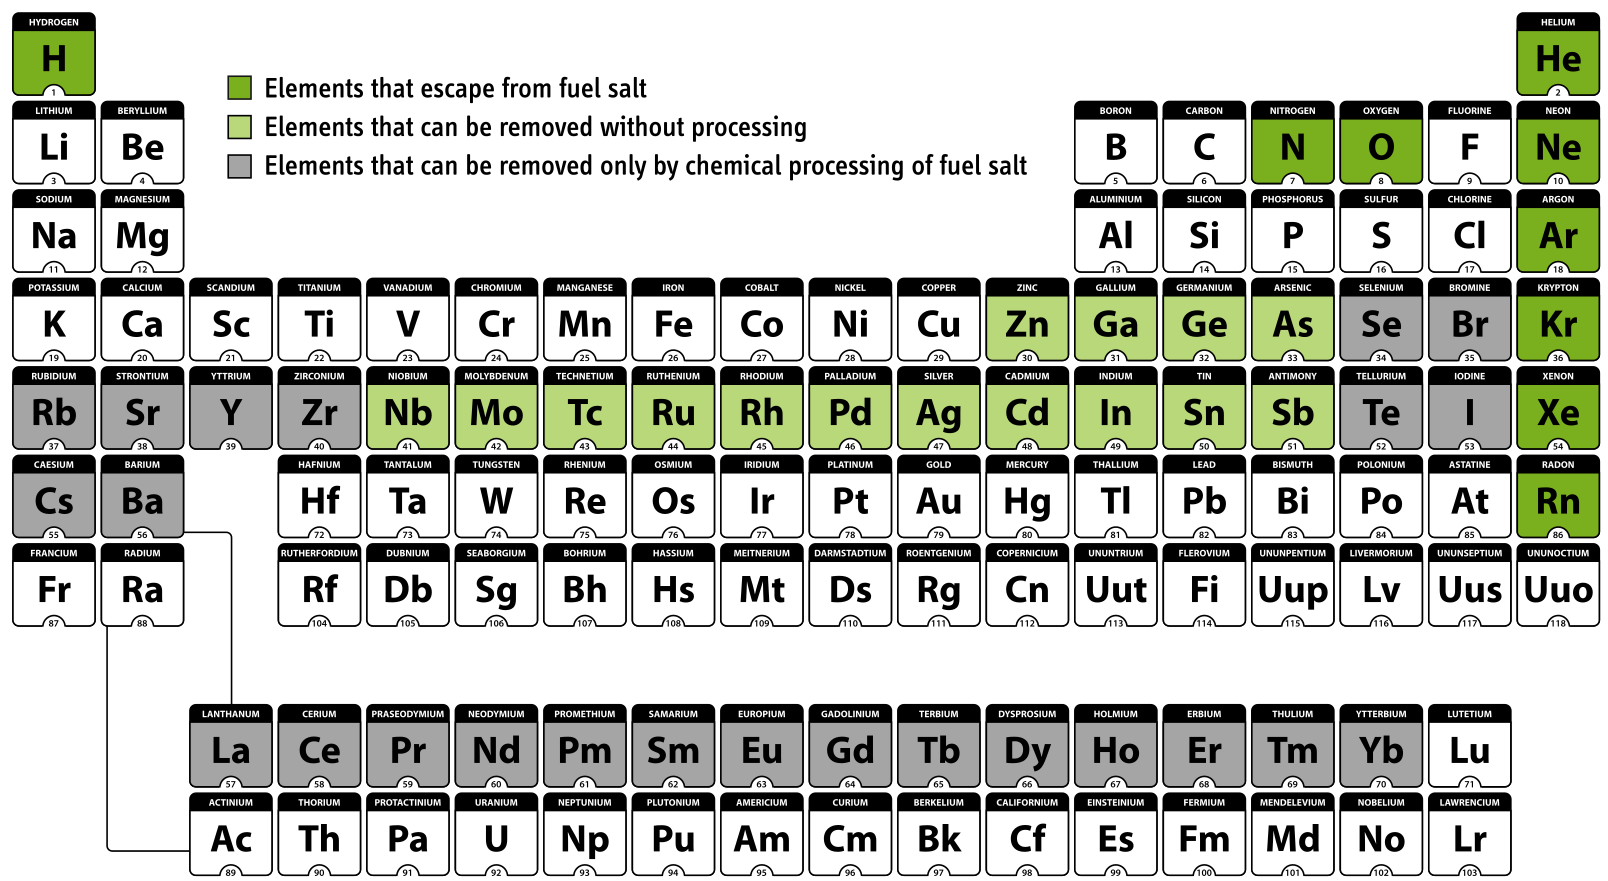
\includegraphics[width=\textwidth]{intr/periodic_map.png}
	\caption{Processing options for \gls{MSR} fuels (reproduced from 
		Ahmed \emph{et al.} \cite{ahmad_neutronics_2015}).}
	\label{fig:periodic_tab}
\end{figure}

Most liquid-fueled nuclear reactor concepts adopt continuous separations 
and feeds: the core material is circulated to or from the core at all times 
(continuously) or specific intervals (batch-wise). In contrast, in a 
solid-fueled reactor, fission products and actinides remain within the initial 
fuel material throughout its time in the core.

The ability to perform online fuel salt reprocessing improves the potential 
neutronics performance of liquid-fueled reactors. First, liquid-fueled 
reactors can operate with relatively low excess reactivity because fissile 
material can be continuously added to the core. Second, continuously removing 
fission products, including strong absorbers (poisons), can significantly 
improve fuel utilization and decrease parasitic neutron absorption. Third, 
online reprocessing decreases the amount of decay heat, dissipating after 
shutdown. Finally, for a breeder\footnote{\gls{CR} 
	$\equiv$ fissile generated/fissile consumed: if CR $<$ 1, the reactor is a 
	``converter''; CR $\equiv$ 1, an ``isobreeder''; CR $>$ 1, a 
	``breeder.''} excess of fissile material might be continuously extracted  
from the core and used to startup new reactors. Nevertheless, the removal of
each element from the liquid fuel salt presents a unique challenge in terms of
chemical separation, storage, and disposal of the separated materials.

Contemporary nuclear fuel depletion software lacks continuous fuel salt 
reprocessing modeling. To handle material flows in potential online removal 
and feed of liquid-fueled systems, early \gls{MSR} simulation methods at 
\gls{ORNL} integrated neutronics and fuel cycle codes (i.e., Reactor Optimum 
Design (ROD) \cite{bauman_rod_1971}) into operational plant tools (i.e., 
Multiregion Processing Plant (MRPP) \cite{kee_mrpp_1976}) for \gls{MSR} fuel 
reprocessing system design. Extensive research in fast and thermal MSR 
analysis has yielded specialized tools for burnup calculations in 
liquid-fueled nuclear systems \cite{fiorina_investigation_2013, 
sheu_depletion_2013, aufiero_extended_2013, heuer_towards_2014, 
park_whole_2015, betzler_molten_2017, betzler_molten_2019}. 
Table~\ref{tab:msr_codes} presents a list of recent efforts, along with the 
main features of the employed methods and software.
\FloatBarrier

\begin{table}[htbp]
	\fontsize{9}{11}\selectfont
	\caption{Tools and methods for liquid-fueled \gls{MSR} fuel salt 	
	depletion analysis.}
	\begin{tabularx}{\textwidth}{p{0.13\textwidth} p{0.18\textwidth} 	
	p{0.18\textwidth} p{0.15\textwidth} p{0.2\textwidth}} 
	\hline
	&Nuttin \emph{et al.}, 2005 \cite{nuttin_potential_2005}& Aufiero 
	\emph{et al.}, 2013 \cite{aufiero_extended_2013} & Betzler \emph{et al.}, 
	2018 \cite{betzler_fuel_2018}&Present work \\ \hline
	Neutronics&\gls{MCNP}&Serpent 2 &SCALE6.2     &Serpent 2 \\
	software  & REM      &          &ORIGEN-S     &			       \\
         	  &stochastic&stochastic&deterministic&stochastic      \\[10pt]
	Geometry  & unit cell& full-core 3D&unit cell&full-core 3D\\      [10pt]
	Removal/feed  & continuous &continuous & batch-wise & batch-wise\\[10pt]
	Separation efficiency &\multicolumn{3}{c}{fixed, must be defined by 
	user before simulation} & function of many para\-me\-ters \\ [10pt]
	Fuel reprocessing plant & \multicolumn{3}{c}{single component, 	``black'' 
	box model} & realistic multi-compo\-nent model \\ [10pt]
	Reactivity control & \multicolumn{2}{c}{continuous adjustment of fissile 
	material injection} & batch injection of fissile material & periodical 
		adjustment of geometry and fissile material injection\\ [10pt]
	Safety parameters evolution & thermal feedback & not considered & thermal 
	feedback & thermal feedback, control rod worth, axial offset \\
	\hline
	\end{tabularx}
	\label{tab:msr_codes}
\end{table}

Two main online reprocessing simulation approaches have been demonstrated in 
the literature: batch-wise and continuous. In the batch-wise approach, the 
burnup simulation stops at a given time and restarts with a new liquid fuel 
composition (after removal of discarded materials and addition of 
fissile/fertile materials). 

\gls{ORNL} researchers have developed ChemTriton, a Python script for
SCALE/TRITON, which employs the batch-wise approach to simulate a continuous 
reprocessing and refill for either single or multiple fluid designs.  
ChemTriton models salt treatment, separations, discharge, and refill using  
SCALE/TRITON depletion simulation over small time steps to simulate continuous 
reprocessing and deplete the fuel salt \cite{betzler_fuel_2018, 
powers_new_2013}.

In the continuous approach, accounting for removal or addition of material 
presents a greater challenge since it requires adding a term to the Bateman 
equations. Both ORIGEN \cite{gauld_isotopic_2011} and the Serpent burnup 
routine \cite{leppanen_burnup_2009} solves a set of the Bateman equations 
using one-group averaged flux and transmutation cross sections obtained from a 
transport calculation. The Bateman equations describe the rate of change of 
each isotope, $i$, due to neutron induced reactions and decay processes
\cite{tsoulfanidis_nuclear_2013}:
\begin{align} \label{eq:bateman}
	\frac{dN_i}{dt} &= \sum_{m=1}^{M}l_{im}\lambda_mN_m + 
	\phi\sum_{m=1}^{M}f_{im}\sigma_mN_m - (\lambda_i + \phi\sigma_i + r_i - 
	f_i)N_i + F_i\Big|{i\in [1,M]}\\
	& \qquad (1) \qquad\qquad\qquad (2) \qquad\qquad(3) \quad (4)  \quad 
	(5) \quad (6)
	\nonumber
	\intertext{where}
	N_i &= \mbox{number density of nuclide \emph{i} $[cm^{-3}]$} \nonumber \\
	M &= \mbox{number of nuclides $[-]$} \nonumber \\
	l_{im} &= \mbox{fraction of decays of nuclide \emph{m} that result in 
	formation of nuclide \emph{i} $[-]$} \nonumber \\
	\lambda_i &= \mbox{radioactive decay constant of nuclide \emph{i} 
	$[s^{-1}]$} 
	\nonumber \\
	\phi &= \mbox{neutron flux, averaged over position and energy 
	$[cm^{-2}s^{-1}]$} \nonumber \\
	f_{im} &= \mbox{fraction of neutron absorption by nuclide \emph{m} 
	leading to the formation of nuclide \emph{i} $[-]$} \nonumber \\
	\sigma_m &= \mbox{average neutron absorption cross section of nuclide 
	\emph{m} $[cm^2]$} \nonumber \\
	r_i &= \mbox{continuous removal rate of nuclide \emph{i} from the 
	system $[s^{-1}]$} \nonumber \\
	f_i &= \mbox{continuous feed rate of nuclide \emph{i} $[s^{-1}]$} 
	\nonumber \\
	F_i &= \mbox{production rate of nuclide \emph{i} directly from 
	fission $[cm^{-3}\cdot s^{-1}]$.}\nonumber
\end{align}
The terms on the right-hand side of the equation represent:
\begin{enumerate}[label=(\arabic*)]
	\item production of species $i$ as a result of the decay of all the 
	nuclides present;
	\item production of species $i$ as a result of neutron capture by all 
	nuclides present;
	\item loss of nuclide $i$ through its own decay;
	\item loss of nuclide $i$ as a result of neutron capture;
	\item loss of nuclide $i$ through continuous removal from the system;
	\item gain of nuclide $i$ as a result of continuous feed to the 
	system.
\end{enumerate} 

Nuttin \emph{et al.} developed an in-house depletion code called \gls{REM}, 
which directly couples with \gls{MCNP} \cite{werner_mcnp_2017-1} to simulate 
fuel salt material evolution in a simplified \gls{MSBR}-like liquid-fueled 
system. That work directly integrated the Bateman differential equations using 
neutron flux from \gls{MCNP}, tracking all the isotopes available in the 
data library, and controlling reactivity to maintain reactor criticality
\cite{nuttin_potential_2005}.

In a similar vein, Aufiero \emph{et al.} extended Serpent 2 for continuous 
reprocessing simulations by adding an explicit pseudo-decay term representing 
fission product removal ($-N_i r_i$ term in Equation~\ref{eq:bateman}) for 
each target poisonous nuclide \cite{aufiero_extended_2013}. The developed 
extension directly accounts for the effects of online fuel reprocessing on 
depletion calculations and features a reactivity control algorithm. The 
extended version of Serpent 2 was assessed against a dedicated version of the 
deterministic ERANOS-based EQL3D procedure in 
\cite{fiorina_investigation_2013} and applied to analyze the \gls{MSFR} fuel 
salt isotopic evolution.

More recently, Betzler \emph{et al.} added to SCALE/TRITON continuous removals 
capability for depletion simulation \cite{betzler_molten_2019}. Similar to 
Aufiero \emph{et al.} this extended SCALE/TRITON directly adds feed and 
removal terms in the burnup matrix and solves it using existing ORIGEN 
capabilities. TRITON's continuous reprocessing capability was validated 
against the batch-wise script ChemTriton for single-channel \gls{MSRE}-like 
model. Unlike ChemTriton, this new capability will be available for all SCALE 
users in the 6.3 release. However, at the moment, it is undergoing extensive 
testing and validation procedures and unavailable for external users.

Some of the tools listed in Table~\ref{tab:msr_codes} used significant  
approximations that may lead to inaccurate fuel evolution predictions and 
others unavailable for external users. This work introduces an 
open-source simulation package, SaltProc, which expands the capability of the 
continuous-energy Monte Carlo Burnup calculation code, Serpent 2, for 
depletion calculations of liquid-fueled \glspl{MSR}.

Most of the existing tools in the literature represented the fuel salt 
reprocessing plant as an invariable ``black box'' model, which removes target 
elements all at once with a fixed efficiency, determined by the user before 
starting the depletion simulation. Typically, such a ``black box'' model is 
characterized by a vector of removing elements and their extraction 
efficiencies:
\begin{align}
&\qquad\qquad\qquad\qquad
\begin{bmatrix}
N^{b}_{0} \\ \vdots \\ N^{b}_{e} \\ \vdots \\ N^{b}_{E} \\
\end{bmatrix} 
\times
\begin{bmatrix}
\epsilon_{0} \\ \vdots \\ \epsilon_{e} \\ \vdots \\ \epsilon_{E} \\
\end{bmatrix} =
\begin{bmatrix}
N^{a}_{0}\\ \vdots \\ N^{a}_{e} \\ \vdots \\N^{a}_{E}  \\
\end{bmatrix} \\
\intertext{where}
N^{b} &= \mbox{number density vector before reprocessing $[cm^{-3}]$} 
\nonumber \\
N^{a} &= \mbox{number density vector after reprocessing $[cm^{-3}]$} 
\nonumber \\
\epsilon &= \mbox{extraction efficiency $[-]$ vector for all elements $e$ in 
$(0,E)$.} \nonumber
\end{align}

The main issues related to static ``black box'' model assumptions in the 
literature neglect: 
\paragraph*{Time varying extraction.} Realistically, long-term reactor 
operation will require a time-dependent extraction efficiency vector. The 
current tools treat separation efficiency as constant.
\paragraph*{The impact of operational parameters on separation efficiency.} In 
reality, the extraction efficiency depends on temperature, power level, 
current fuel salt isotopic composition, and material mass flow rate. Gas 
solubility in the salt is inversely proportional to the salt temperature; 
hence, the extraction efficiency expected to be lower for the higher 
temperature of the salt.
\paragraph*{Discrete component performance and dynamics in the multi-component 
system.} All reprocessing plant components are treated as a single ``black 
box'' component in existing simulation tools. However, the fuel salt in a 
reprocessing plant undergoes many separate components (e.g., helium bubbling, 
nickel mesh filter, etc.) that target specific elements. Some of these 
components can be connected in series, parallel, or series-parallel. The 
``black box'' model (only single process) requires extensive pre-simulation 
analytic work from the user to calculate the lumped separation efficiency 
vector before a simulation is run and cannot be adjusted during the 
simulation. Additionally, treating the processing system as a single ``black 
box'' neglects dynamics related to relative component flow rates. Finally, the 
discrete waste streams from each component are not tracked separately in 
``black box'' tools. However, this information is necessary for fuel 
reprocessing system optimization.\\

In contrast with tools listed in Table~\ref{tab:msr_codes}, SaltProc, does not 
make these approximations. SaltProc allows the user define the separation 
efficiency as a function of time or operational parameters, and is able to 
simulate multi-component fuel reprocessing system instead of ``black box''.

\section{Operational and safety parameter evolution} 
\label{sec:saf-par-literature}
In contrast with conventional solid-fueled reactors with in-core fuel 
residence averaging 4-5 years\footnote{For the typical 18-month cycle, during 
refueling personnel removing 1/3 of the fuel assemblies, re-arranging other 
assemblies, and loading fresh fuel into the core. Thus, each fuel assembly is 
kept in the core at most $3\times 18=54$ months.}, an initial \gls{MSR} fuel 
salt batch stays in the \gls{MSR} primary loop throughout the reactor 
lifetime. 
Therefore, the fuel salt accumulates \glspl{FP} not captured by the fuel 
reprocessing system as well as transuranic elements\footnote{The chemical 
elements with atomic numbers greater than uranium (92).}. Continuous fuel 
salt composition evolution has a significant influence on the neutron energy 
spectrum and, consequently, affects the reactor behavior, necessitating 
additional safety analysis.

Nuttin \emph{et al.} studied the evolution of a key safety parameter, the 
temperature reactivity feedback coefficient, estimating it for the \gls{MSBR} 
at startup and equilibrium. The temperature coefficient of reactivity 
quantified reactivity changes due to temperature increase in the core and was 
calculated in that work as:
\begin{align}\label{eq:feedback}
	&\qquad\qquad \alpha = \frac{k_{1200} - k_{900}}{\delta 
	T} \\
	\intertext{where}
	k_{900}, k_{1200}  &= \mbox{multiplication coefficients at 900K and 
		1200K $[-]$} \nonumber \\
	\delta T &= \mbox{300 $[K]$.}\nonumber
\end{align}

That work showed that the \gls{FTC} at startup and equilibrium is $-1.5$ 
and $-1.0$ $pcm/K$, respectively\footnote{ 1 pcm = 10$^{-5}\Delta 
k_{eff}/k_{eff}$}. Nuttin \emph{et al.} also reported a positive and 
time-invariant total temperature coefficient ($+0.8$ $pcm/K$) 
\cite{nuttin_potential_2005}. Recently, Park and colleagues expanded that 
approach to a full-core high-fidelity \gls{MSBR} model and estimated safety 
parameters evolution over 20 years of operation \cite{park_whole_2015}. These 
calculations showed a relatively large negative total temperature coefficient 
during the 20 year reactor operation. DUring that time, the coefficient 
magnitude weakens from $-3.21$ to $-1.41$ $pcm/K$ from startup to equilibrium, 
respectively. Additionally, that work reported a control rod worth 
deterioration from $2099pcm$ to $1970pcm$ due to neutron spectrum hardening 
during reactor operation. 

More recently, Betzler \emph{et al.} \cite{betzler_assessment_2017-1} reported 
safety parameter evolution for the \gls{TAP} \gls{MSR}: the fuel 
reactivity coefficient at \gls{BOL} and 15 years from \gls{BOL} was negative 
and decreasing slowly over the reactor lifetime (from -4.0 to -4.1 $pcm/K$ 
when temperature was perturbed from 900K to 1200K); the moderator reactivity 
coefficient was +0.43 $pcm/K$ at \gls{BOL} and -2.7 $pcm/K$ after 15 
years of operation. Overall, thermal feedback seems to be stronger in the 
\gls{TAP} reactor and deteriorates insignificantly during the reactor 
operation. Notably, the authors ignored material density change with 
temperature to simplify temperature coefficient calculation; thus, only  
Doppler broadening was taken into account. The researchers reported the total 
worth of all control rods in the \gls{TAP} core only for the startup fuel 
composition. 

The evolution of control rod worth in the \gls{TAP} has not been reported in 
the literature before. Chapter 5 of this dissertation illuminated the 
evolution of essential safety parameters (fuel, moderator, total temperature 
coefficient, control rod worth) for the \gls{TAP} \gls{MSR} at various moments 
during the reactor operation. Additionally, I investigated the impact of 
neutron poison accumulation (e.g., $^{135}$Xe) in the fuel salt during 
short-term transients (i.e., load following) on major safety characteristics 
\cite{rykhlevskii_impact_2019}.


\section{Background Summary}
State-of-the-Art software packages for depletion analysis and evolution of 
safety parameters in the liquid-fueled \gls{MSR} are reviewed in 
Section~\ref{sec:litreview}. Based on this summary, I have identified a few 
possible directions for the improvement of \gls{MSR} tools:
\paragraph*{Reproducibility/availability.}
Serpent is the only contemporary nuclear reactor physics software that can 
perform depletion calculations that can take into account online fuel salt 
reprocessing regimes. However, this built-in online reprocessing routine is 
undocumented: the discussion forum for Serpent users is the only useful 
source of information at the moment. Other mentioned tools are available for 
internal users only. These issues can be a barrier to reuse research software 
and to reproduce scientific results. Thus, a new, open-source, reproducible 
tool for fuel processing simulation would assist in the production of 
reproducible research in the area of liquid-fueled reactor modeling.
\paragraph*{Realistic fuel reprocessing system model.} 
Significant approximations in fuel reprocessing parameters deteriorate fuel 
salt composition predictions since the evolution of safety parameter accuracy 
is strongly dependent on fuel salt composition. A realistic fuel reprocessing 
system model will allow reprocessing component parameter optimization,  
increase the fidelity of fuel and waste stream composition calculations, and 
advance reprocessing system design.
\paragraph*{Variable extraction efficiency.} Most research efforts in 
the literature (except Nuttin \emph{et al.}\footnote{Nuttin \emph{et al.} 
assumed 100\% extraction efficiency for noble gases (Xe, Kr) and protactinium, 
20\% for rare earths, 5\% for semi-noble metals, and 1\% for alkaline 
elements \cite{nuttin_potential_2005}.}) assume ideal 100\% extraction 
efficiency of all removed 
elements, which stayed constant during the whole reactor lifetime. 
Realistically the efficiency is time-dependent and changes with respect to 
operational parameters: temperature, power level, salt composition, etc. Thus, 
the ability to set up dynamic separation efficiency must be added in \gls{MSR} 
simulation tools to advance depletion calculations.
\paragraph*{Reactivity control.} Reconfigurable moderator configuration in the 
\gls{TAP} core presents a challenge because of the core geometry changes with 
time. The reactivity control module, which adjusts the core geometry 
to maintain criticality, would be an exceptional capability for simulating  
new, more advanced \gls{MSR} concepts and short-term transients.
\paragraph*{Safety characteristics evolution during reactor operation.} The 
\gls{MSR} fuel salt  accumulates \glspl{FP} and transuranic elements, which 
significantly shift the neutron energy spectrum. This spectrum shift might 
worsen the core safety during operation. The impact of the fuel salt 
evolution on the \gls{MSR} safety parameters must be carefully investigated 
and reported.\\

This work aims to overcome these issues and demonstrate the tool capabilities 
for a two promising \gls{MSR} concepts.


\section{Objectives and outline of the work}
Most of the existing \gls{MSR} depletion simulators usually assume ideal  
efficiency (100\% of the target nuclide is being removed) of the neutron 
poison removal process (see Section~\ref{sec:litreview}). The main goal of 
this dissertation is to develop a generic open-source tool, SaltProc, capable 
of simulating a wide range of liquid-fueled systems --- including multi-fluid 
and multi-region designs --- and validate it against existing modeling 
efforts. Additionally, SaltProc enables poison extraction simulation based on 
a realistic physics-based fuel processing model. 

The structure of the thesis is as follows. Chapter 1 serves as a literature 
review, providing background on fuel burnup, online fuel reprocessing  
approaches, safety parameter evolution during reactor operation, and how these 
concepts have been applied to a wide range of \glspl{MSR} in the literature. 
Chapter 2 details online reprocessing modeling and the proposed computation 
tool architecture. In an attempt to avoid the pitfalls of a ``black box''  
understanding and to identify method limitations at an early stage, governing 
equations and working principles are stated and discussed. Chapter 3 presents 
equilibrium-seeking results for the \gls{MSBR} as well as essential 
operational and safety parameters for both the initial and equilibrium states.

Additionally, the benefits of continuous fission product removal for a thermal 
\gls{MSR} are evaluated at the end of chapter 3. Chapter 4 covers SaltProc 
demonstration and validation efforts with a focus on the \gls{TAP} \gls{MSR},  
taking into account adjustable moderator configuration. Chapter 5 gives the 
safety parameter overview and its evolution during the \gls{TAP} 
lifetime-long reactor operation. Moreover, the safety parameters dynamics 
during short-term transients have been evaluated at the end of chapter 5. The 
final chapter summarizes this work's contribution to the nuclear community, 
and a conclusion is offered together with an outlook for future work on the 
topic.	% for INTRODUCTION in "intro.tex"
\chapter[Online reprocessing modeling approach]{Online reprocessing modeling 
approach}
\section{Fuel salt reprocessing overview} \label{sec:reproc-plant}
Removing specific chemical elements from a molten salt is a complicated 
task that requires intelligent design (e.g., chemical separations equipment 
design, fuel salt flows to equipment). This section contains a brief overview 
of a generic \gls{MSR} fuel salt reprocessing system. Modeling such systems is 
the focus of current dissertation.

\subsection{Gas separation system} \label{sec:gas-separ}
Gaseous fission products (e.g., Kr, Xe) must be removed from the fuel salt 
to avoid reactor poisoning, especially during startup and power maneuvering. 
This is particularly true for $^{135}$Xe, with its extensive neutron capture 
cross section ($\approx10^6\dots10^7$ b in a thermal energy range). $^{135}$Xe 
is produced directly from fission in about 0.3\% of $^{235}$U fissions 
($\gamma_{_{^{135}Xe}}$), but an even larger fraction of $^{135}$Xe is 
produced by the decay of $^{135}$I and $^{135}$Te (table~\ref{tab:xe_gain}). 
$^{135}$I and $^{135}$Te yields from fission are 
$\gamma_{_{^{135}I}}\!=3.6$\% and $\gamma_{_{^{135}Te}}\!=2.5$\%, 
respectively. Thus, total $^{135}$Xe production  
from fission is about 6.4\% of fissions (of $^{235}$U), most of this is from 
$^{135}$I and $^{135}$Te decay. Noble gases (e.g. tritium, xenon, and krypton) 
can 
be removed from the fuel salt as follows:
\begin{enumerate}[label=(\alph*)]
	\item a bubble generator injects helium bubbles in the salt stream;
	\item noble gases migrate promptly to the helium bubbles because 
	of their extreme insolubility in the salt 
	\cite{robertson_conceptual_1971};
	\item and a gas separator discharges the fission-product-rich bubbles from 
	the salt to the off-gas system.
\end{enumerate}
%%%%%%%%%%%%%%%%%%%%%%%%%%%%%%%%%%%%%%%%%%%%%%%%%%%%%%%%%%%%%
\begin{table}[ht!]
	\caption{$^{135}$Xe production sources and principal rate constants 
		involved
		(reproduced from Kedl \emph{et al.} \cite{kedl_development_1967}).}
	\centering
	\begin{tabularx}{\textwidth}{b  b}
		\hline \textbf{$^{135}$Xe gain mechanism} & \textbf{Principal rate 
			parameters involved}  	\\ [5pt] \hline 
		Direct from fission & $\Sigma_f \gamma_{_{^{135}Xe}}\phi$ (for 
		$^{235}$U fission) \\
		yield $\gamma_{_{^{135}Xe}}\!\!\!=0.003$ & \\ [5pt] \hline 
		$^{135}$I decay     & $\Sigma_f \gamma_{_{^{135}I}}\phi$ (for 
		$^{235}$U fission) \\
		yield $\gamma_{_{^{135}Xe}}\!\!\!=0.036$, it decays to $^{135}$Xe with 
		$\tau_{1/2}=6.68$ h & 			                    \\	[5pt]	\hline 
		$^{135}$Te decay    & $\Sigma_f \gamma_{_{^{135}Te}}\phi$ (for 
		$^{235}$U 		fission) \\
		yield $\gamma_{_{^{135}Xe}}\!\!\!=0.025$, 
		it decays to $^{135}$I with $\tau_{1/2}=19$ s 
		& 			                    \\ [5pt]	\hline
	\end{tabularx}
	\label{tab:xe_gain}
\end{table}
%%%%%%%%%%%%%%%%%%%%%%%%%%%%%%%%%%%%%%%%%%%%%%%%%%%%%%%%%%%%%%%%%%%
Diagram~\ref{fig:xe_diagram} shows the key pathways for xenon production, 
accumulation, and removal in a typical \gls{MSR}. 
Figure~\ref{fig:gas_removal_system} shows the principal design of the  
\gls{MSBR} gas separation system. Helium bubbles of a specific size are 
introduced in a salt stream via the primary pump bowl. These bubbles absorb 
noble gases before being separated from the salt by a gas separator. 
\gls{ORNL} suggested that the \gls{MSBR} off-gas system would inject 
$d=0.508$mm helium bubbles in the pump bowl, redirect 10\% of the fuel salt 
flow through a bubble separator to remove the bubbles, and then return the 
flow back into the pump suction. Robertson \emph{et al.} reported that helium 
bubble size was approximately 25\% of the throat width (blue circle on 
figure~\ref{fig:bubble_separator}) and was independent of the gas flow rate 
\cite{robertson_conceptual_1971}. Consequently, it is possible to regulate the 
helium bubble size by changing the throat width in the bubble generator.
\begin{figure}[htp!] % replace 't' with 'b' to 
	\centering
	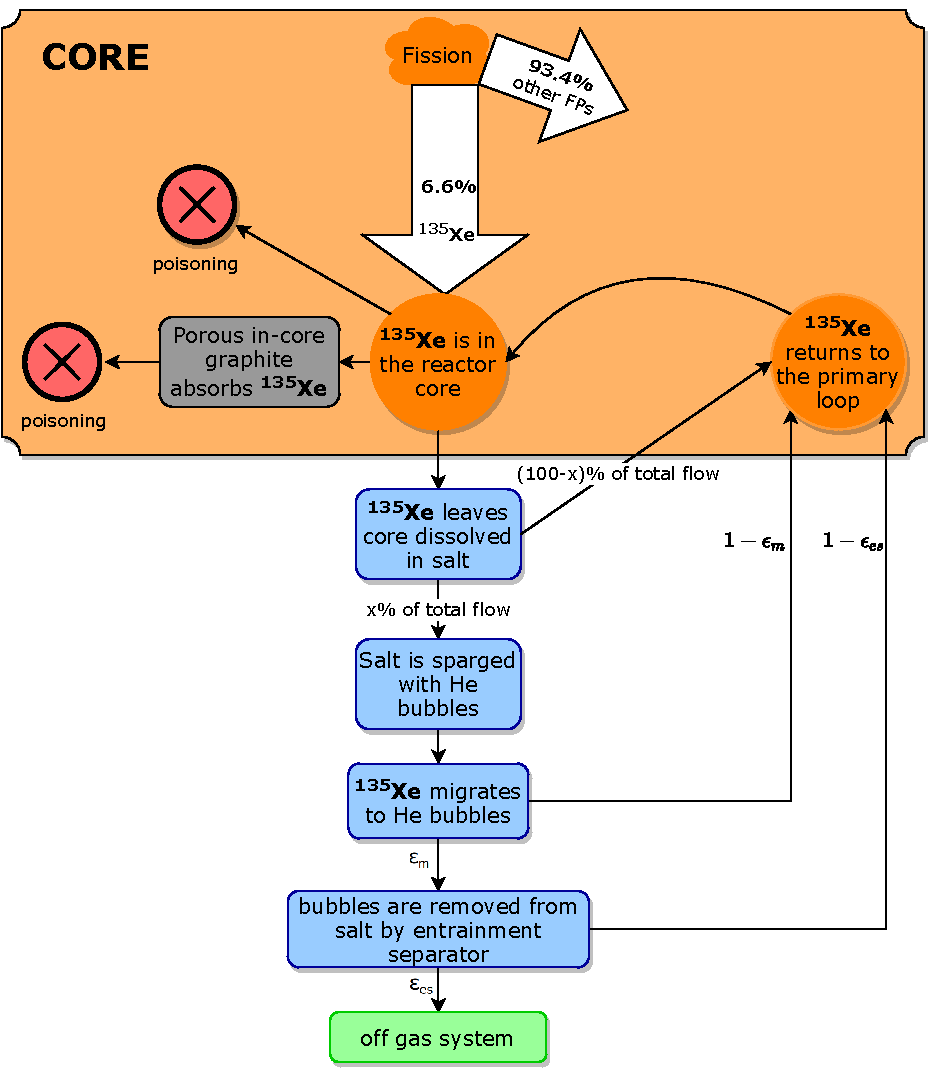
\includegraphics[width=1.01\textwidth]{ch2/xe_diagram.pdf}
	\caption{Schematic of $^{135}$Xe circulation in a generic \gls{MSR}. $x$ 
	is the fraction of fuel salt flow from the pump discharge redirected to 
	the gas separation system, while $\epsilon_m$ and $\epsilon_{es}$ are the 
	efficiencies of migration (of $^{135}$Xe to the helium bubbles in the 
	sparger) and separation (of gas in the entrainment separator), 
	respectively. The orange color represents the fuel salt in the primary 
	loop, the blue color represents the gas separation system, and the gray 
	color is moderator in the core. Fission yields assume $^{235}$U fission 
	only.}
	\label{fig:xe_diagram}
\end{figure}
\begin{figure}[htp!] % replace 't' with 'b' to 
	\centering
	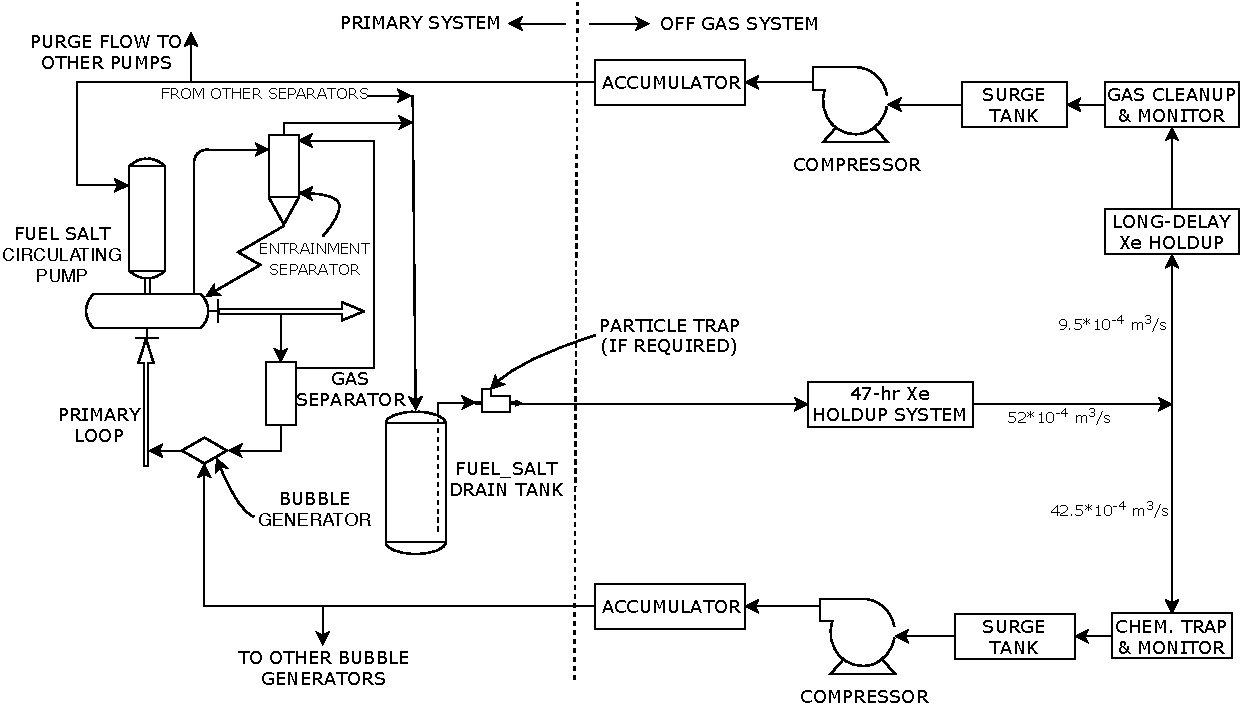
\includegraphics[width=1.02\textwidth]{ch2/gas_separation.pdf}
	\caption{Schematic flow diagram of the \gls{MSBR} gas separation system 
		(figure reproduced from Robertson \emph{et al.} 
		\cite{robertson_conceptual_1971}).}
	\label{fig:gas_removal_system}
\end{figure}
\begin{figure}[htp!] % replace 't' with 'b' to 
	\centering
	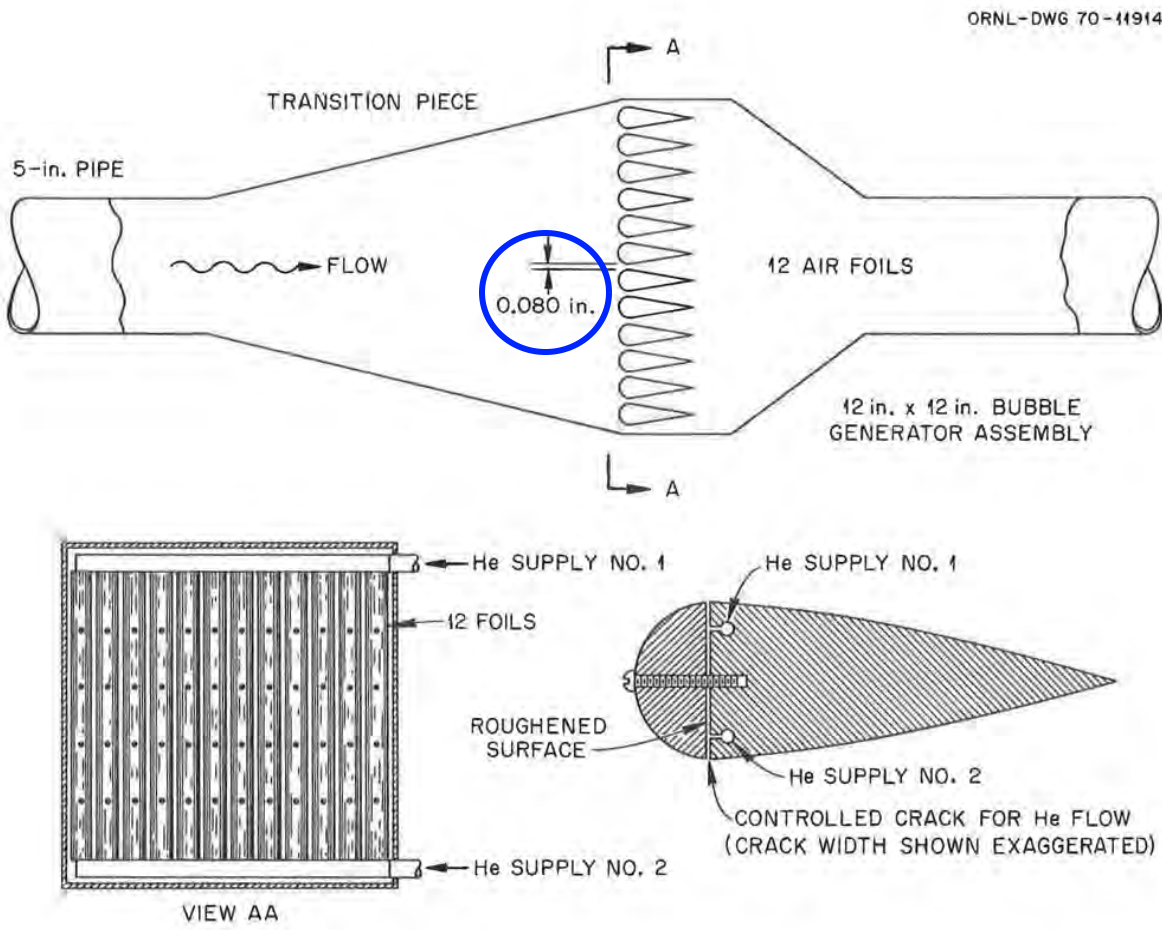
\includegraphics[width=0.77\textwidth]{ch2/msbr_bubble_generator.png}
	\caption{Preliminary concept of \gls{MSBR} bubble generator (figure 
		reproduced from Robertson \emph{et al.} 
		\cite{robertson_conceptual_1971}). 
		The blue circle shows throat width, which determines bubble size.}
	\vspace{-0.25in}
	\label{fig:bubble_separator}
\end{figure}
\begin{table}[b]
	\caption{$^{135}$Xe loss terms and principal rate constants involved
		(reproduced from Kedl \emph{et al.} \cite{kedl_development_1967}).}
	\centering
	\begin{tabularx}{\textwidth}{b b}
		\hline \textbf{$^{135}$Xe loss mechanism}      & \textbf{Principal 
			rate 
			parameters involved}  	\\
		\hline Decay of dissolved $^{135}$Xe ($\tau_{1/2}=9.1$ h)  & Decay 
		constant	($\lambda$)		\\
		\hline $^{135}$Xe burnup              &  Neutron flux 
		($\phi$)		 					\\
		dissolved xenon-135 burnup as it passes throught core  
		& 			            \\		\hline $^{135}$Xe migrated to 
		helium bubbles & Removal efficiency 
		($\epsilon_m$)		\\
		\hline $^{135}$Xe transferred into circulating He bubbles; this xenon 
		will eventually be burnup, decay, or stripped via bubble separator & 
		Mass transfer coefficient ($h$), decay constant ($\lambda$), 
		neutron flux ($\phi$), bubble removal efficiency 
		($\epsilon_{es}$)		\\
		\hline 
	\end{tabularx}
	\label{tab:xe_loss}
\end{table}

To realistically model the gas separation system, we need a mathematical model 
which describes noble gas extraction efficiency during reactor operation. 
Particularly, a model of xenon extraction efficiency as a function of sparger 
design parameters is needed to accurately model $^{135}$Xe removal in a fuel 
salt depletion simulation. The gain and loss terms for $^{135}$Xe dissolved in 
the fuel salt are listed in Tables~\ref{tab:xe_gain} and \ref{tab:xe_loss}. 
The removal efficiency for the xenon in the pump bowl was measured during 
\gls{MSRE} operation, but the technical report ORNL-4069 by Kedl-Houtzeel only 
stated its range (from 50 to 100\%) and concluded, ``It is probably a 
complex parameter like the circulating-void fraction and depends on many 
reactor operational variables.'' \cite{kedl_development_1967}. $^{135}$Xe 
burnup and decay rates are well known. 

Peebles \emph{et al.} in ORNL-TM-2245 has reported xenon removal efficiency 
($\epsilon_{Xe}$) in a gas separation system as a function of many parameters 
\cite{peebles_removal_1968}:
\begin{align}\label{eq:gas_eff}
& \qquad\qquad \epsilon_{Xe} = \frac{1-e^{-\beta}}{1+\alpha}
\intertext{where}
\alpha &= \frac{RTQ_{salt}}{HQ_{He}} \\
\beta &= \frac{K_L a A_C L (1+\alpha)}{Q_{salt}} \\
R &= \mbox{universal gas constant} \nonumber \\
T &= \mbox{salt temperature} \nonumber \\
Q_{salt}&= \mbox{volumetric salt flow rate} \nonumber \\
Q_{He}&= \mbox{volumetric helium flow rate} \nonumber \\
H &= \mbox{Henry's law constant for solute gas} \nonumber \\
a &= \mbox{gas-liquid interfacial area} \nonumber \\
A_C &= \mbox{contactor cross section} \nonumber \\
L &= \mbox{contactor length} \nonumber \\
K_L &= \mbox{liquid phase mass transfer coefficient.} \nonumber
\end{align}
Most of the input parameters for that correlation are obvious and easy to 
obtain from the system component design. The mass transfer coefficient for 
transferring xenon into helium bubbles ($K_L$) can be estimated  
experimentally, but published information is currently insufficient 
to inform an accurate mathematical model appropriate for \gls{CFD}. Thus, 
Peebles \emph{et al.} reported the mass transfer coefficient correlation for 
the \gls{MSBR} salt (LiF-BeF$_2$-ThF$_4$-UF$_4$) but for a limited case. While 
it is out of the scope of this work to accurately estimate mass transfer 
coefficient, this work seeks to provide a tool which would allow the user to 
specify any mathematical model for a separation efficiency.

Equation~\ref{eq:gas_eff} would apply to other noble gases (e.g., Kr, Ar) but 
the Henry's law constant ($H$) and the mass transfer coefficient ($K_L$) would 
be different. Current effort at the University of Illinois at Urbana-Champaign 
namely, ``Enabling Load Following Capability in the Transatomic Power 
\gls{MSR}" \cite{huff_enabling_2018}, has a goal to determine mass transfer 
coefficients for various gaseous fission products (Ar, Kr, Xe) using 
experiments, enabling \gls{CFD} and multiphysics simulations of such reactors. 
As a result, the obtained mathematical model for gas removal efficiency might 
be employed to inform a realistic physics-based fuel reprocessing model in 
SaltProc.


\subsection{Insoluble fission products filtering}
Decay chain of approximately 40\% of fission products has a gaseous elements 
in it. Some of non-gaseous \glspl{FP} produced in the \gls{MSR} core (e.g., 
noble and semi-noble metals) have very low solubility in the molten salt. Some 
fraction of noble and semi-noble solid fission products plate out onto the 
internal surfaces of the primary loop equipment, complicating their removal 
\cite{briggs_molten-salt_1964}. The remains noble and semi-noble metals can be 
removed along with with corrosion products using mechanical filtration system 
which ``consists largely of a high surface area mechanical filter, likely an 
nickel mesh, to promote deposition of suspended, undissolved fission and 
corrosion products,'' stated Holcomb \emph{et al.} 
\cite{holcomb_instrumentation_2018}. The filter is manufactured from porous 
metal and located on a recirculating side stream of the side. The filter has 
limited capacity, needs periodic replacement, and the dose rate on the used 
filter is very high due to the undissolved fission products and residual 
fuel salt remaining on the filter \cite{mcfarlane_review_2019-1}. Differential 
pressure measurements before and after filters are required to determine when 
the filters are full. 

The historic \gls{MSRE} program provided basic information on the design and 
performance of large mechanical filter. Figure~\ref{fig:large_filter_layout} 
shows the piping layout of the filter, storage and processing tanks. The 
filter pressure vessel is made of high-nickel alloy (Inconel) and accommodate 
40-$\mu m$ pore size sintered Inconel fibers. This large molten salt filter 
had total filtering area 0.8${m^2}$ and was designed to filter approximately 
1 kg of the molten salt per minute but the removal efficiency has never been 
reported. Also, the design of the filter, the filter holder, and the 
remotely operated equipment for the filter replacement for commercial-scale 
\gls{MSR} designs presents a significant engineering challenge 
\cite{mcfarlane_review_2019-1}.
\begin{figure}[htp!] % replace 't' with 'b' to 
	\centering
	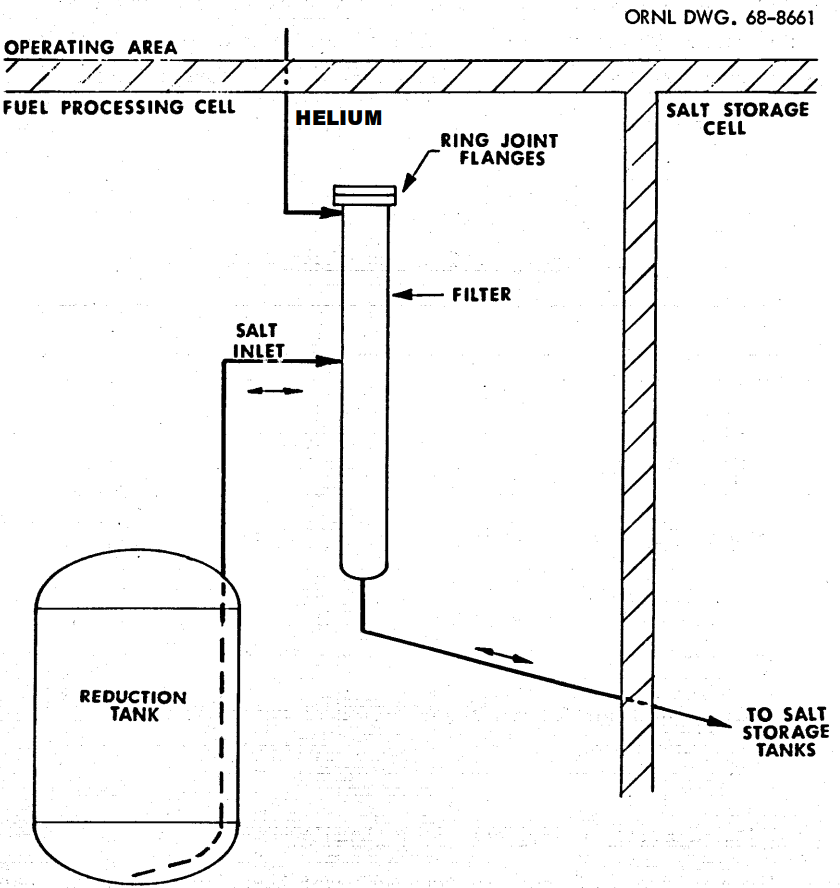
\includegraphics[width=.75\textwidth]{ch2/large_molten_salt_filter_layout.png}
	\caption{Schematic flow diagram of large molten salt mechanical filter 
		designed and operated during the \gls{MSRE} (figure reproduced from 
		Lindauer \emph{et al.} \cite{lindauer_design_1969}).}
	\label{fig:large_filter_layout}
\end{figure}

In this work, separation efficiency in the filtering system is assumed to be 
ideal and constant over reactor operation but in the future work 
physics-driven mathematical formula can be used when the experimental data or 
analytical model will be available.


\subsection{Fuel chemical processing facility} \label{sec:chemical_processing}
In addition to noble gases, noble and semi-noble metals, the fuel salt 
reprocessing system must extract other \glspl{FP} such as lanthanides. These 
absorb fewer neutrons than $^{135}$Xe, but their removal is crucial to 
guarantee normal operation. Meanwhile, lanthanides have relatively high 
solubility in the carrier salt and must be removed by chemical extraction. 

In thorium-fueled \gls{MSR} designs, $^{232}$Th in the fuel salt absorbs 
thermal neutrons and produces $^{233}$Pa which then decays into the fissile 
$^{233}$U (figure~\ref{fig:th_u_reaction}). Protactinium presents a challenge, 
since it has a large absorption cross section in the thermal energy spectrum. 
Accordingly, $^{233}$Pa is continuously removed from the fuel salt into a 
protactinium decay tank to allow $^{233}$Pa to decay to $^{233}$U without 
poisoning the reactor. This feature allows the thorium-fueled \gls{MSR} to 
avoid neutron losses to protactinium, keeps fission products to a very low 
level, and increases the efficiency of $^{233}$U breeding. 

\begin{figure}[htp!] % replace 't' with 'b' to 
	\centering
	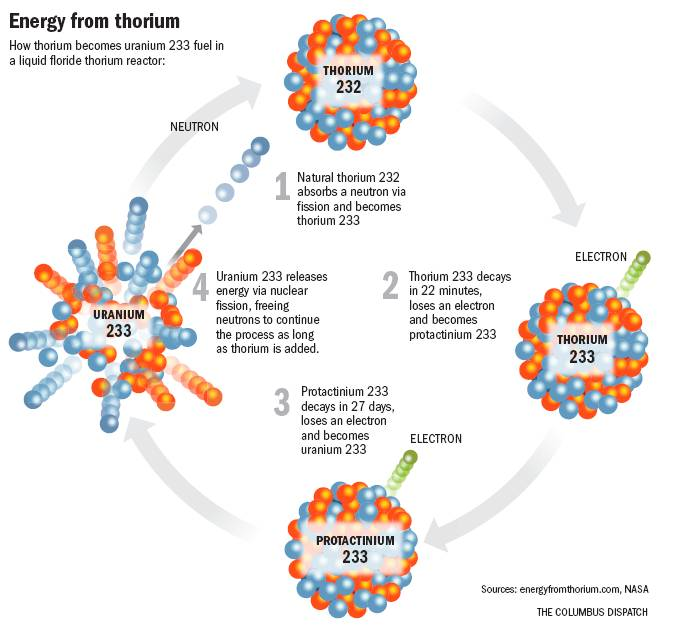
\includegraphics[width=0.57\textwidth]{ch2/th_u_cycle.jpg}
	\caption{Production of $^{233}$U from $^{232}$Th  (reproduced from 
	Sorensen \cite{sorensen_one-fluid_2006}).}
	\label{fig:th_u_reaction}
\end{figure}

Many authors report that a liquid-liquid reductive extraction process is the 
best option for removing protactinium and soluble fission products from 
molten fluoride salts \cite{briggs_molten-salt_1969, delpech_molten_2010, 
	doligez_coupled_2014}. In that process, the protactinium or lanthanides 
	can be 
selectively stripped from the salt into liquid bismuth due to different 
chemical potentials. Moreover, the \gls{MSRE} experience indicated that the 
extraction could be carried out rapidly and continuously  
\cite{whatley_engineering_1970}.

The principal scheme of the \gls{MSBR} reprocessing facility concept is shown 
in Figure~\ref{fig:material_flow}. The fuel salt is first temporarily stored 
for cooling and decay of the shortest-lived fission products, then it is 
directed to the primary fluorinator. There, most of the uranium is removed by 
fluorination to UF$_6$. After that, the salt is routed to an extraction column 
where it is combined with a mixture containing metallic bismuth, lithium, and 
thorium reductants. The remaining uranium and protactinium is  reductively 
extracted to a bismuth solution, leaving a salt that only contains fission 
products dissolved in carrier salt (base composition LiF-BeF$_2$-ThF$_4$). The 
salt then goes through a reduction column where UF$_6$ is reduced to UF$_4$ 
preparing it for return to the reactor. BeF$_2$ and ThF$_4$ are also added, 
and all residual bismuth is removed from the salt. After a final cleanup step 
and valence adjustment, the purified salt returns to the reactor 
\cite{carter_design_1972, sorensen_one-fluid_2006}.

\begin{figure}[htp!] % replace 't' with 'b' to 
	\centering
	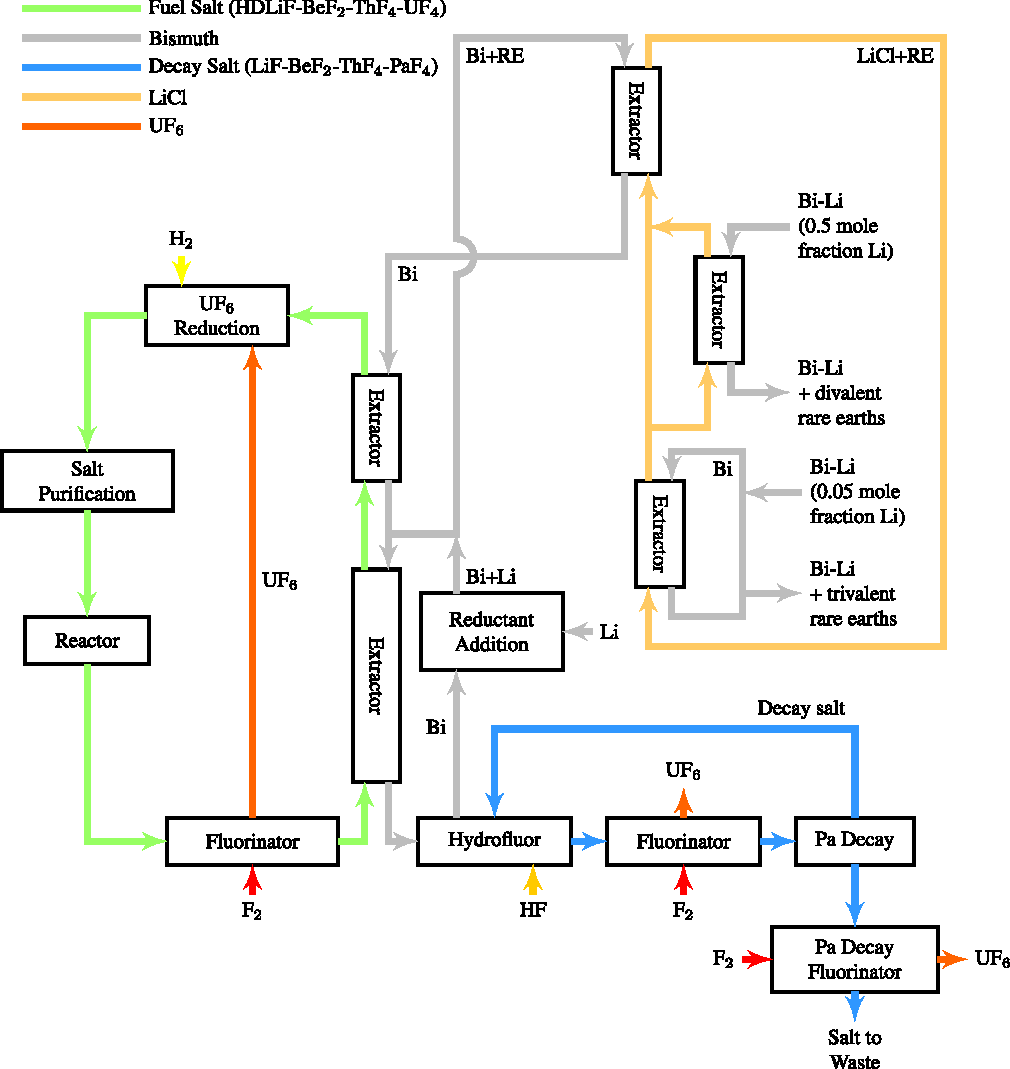
\includegraphics[width=1.01\textwidth]{ch2/flowsheet.pdf}
	\caption{Simplified block diagram of chemical processing scheme for 
		single-fluid \gls{MSBR} (reproduced from Sorensen 
		\cite{sorensen_one-fluid_2006}). \emph{RE} represents the rare 
		earth elements extracted from the salt.}
	\label{fig:material_flow}
\end{figure}

The bismuth accommodating some uranium and protactinium is routed to a 
hydrofluorination column where metallic solutes in the bismuth are oxidized 
into their fluoride forms in the presence of a decay salt\footnote{The decay 
salt contains UF$_4$, PaF$_4$, ThF$_4$ and fission products. Uranium produced 
after $^{233}$Pa decay is extracted and directed back into the reactor. Decay 
salt is the precursor for the waste salt as it was periodically discarded  
every 220 days \cite{robertson_conceptual_1971}.}. The decay salt, containing 
UF$_4$, PaF$_4$, and ThF$_4$, passes into a decay tank where $^{233}$Pa is 
decays to $^{233}$U. The uranium generated by protactinium decay is removed 
through fluorination to UF$_6$ and directed to the reduction column to refuel 
the purified fuel salt. A  hydrofluorinator and a fluorinator can remove 
approximately 95\% of the uranium from the stream 
\cite{robertson_conceptual_1971}.

The fully processed salt, on its way back to the reactor, has uranium added 
from the protactinium decay tank at the rate required to maintain or adjust 
the uranium concentration in the reactor (and, consequently, control the 
reactivity). Adding fissile material is performed by sparging the salt with 
UF$_6$ and hydrogen to produce UF$_4$ in the salt and HF gas 
\cite{robertson_conceptual_1971}.

After these separation steps, the fuel salt stream from the protactinium 
isolation system contains only traces of protactinium and uranium but contains 
practically all of the rare earths. A fraction of this salt stream is 
redirected to a reductive extraction process for removing rare earths.  The 
principal scheme of a rare earth removal system is shown in  
Figure~\ref{fig:rare-earth-removal}. A molten salt flow which contains 
rare earth fluorides is fed to the center of an extraction column. The salt 
flows countercurrent to a liquid bismuth stream which contains thorium and 
lithium. In the upper part of the column, the rare earths are reduced and 
transferred to the downflowing liquid metal stream. Below the feed point, the 
rare earth concentration is increased in the salt and metal streams in order 
to produce a concentration high enough for disposal 
\cite{briggs_molten-salt_1969}.
\begin{figure}[htbp!]
	\centering
	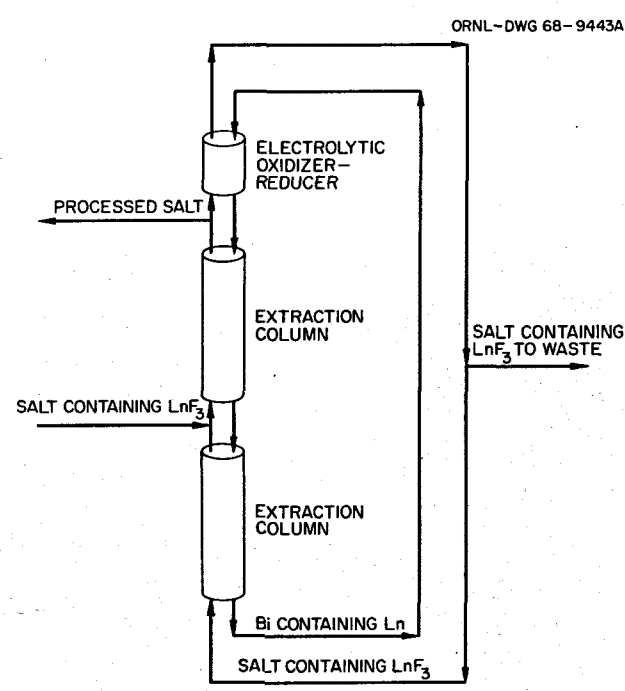
\includegraphics[width=0.45\textwidth]{ch2/rare-earths-removal-system.png}
	\caption{Rare earth removal from a fuel salt by reductive extraction 
		(figure reproduced from Briggs \emph{et al.} 
		\cite{briggs_molten-salt_1969}).}
	\label{fig:rare-earth-removal}
\end{figure}

While it is out of the scope of this work to derive the accurate  
chemistry-based mathematical formula for rare earths and protactinium 
separation efficiency, this work seeks to provide a flexible tool that is able 
to simulate chemical processes in significant detail with regard to key system 
design parameters.

\section{Serpent overview}
Serpent is a continuous-energy Monte Carlo neutronics software capable of 
solving the neutron transport problem by tracking individual neutrons within 
the problem geometry and using stochastic method to determine chain of events 
for each neutron \cite{leppanen_serpent_2014}. Serpent is under active 
development at the VTT Technical Research Centre of Finland since 2004, where 
it was initially conceived as a tool to simplify group constant generation in 
a high-fidelity Monte Carlo environment. Serpent is now a widely used  
transport code, used by more than 500 registered individuals in 155 
organizations located in 37 countries around the world. The burnup calculation 
capability in Serpent is based on built-in calculation routines, without using 
any external solvers. A restart feature enables fuel shuffling simulation or 
applying any modifications to the input by dividing the calculation into 
several parts, which is crucial for online reprocessing simulations.

The latest version, Serpent 2, supports advanced geometries and has advanced 
burnup capabilities, including online refueling capabilities which are 
necessary for neutronic computations of pebble-bed reactors and liquid-fueled 
\glspl{MSR} \cite{aufiero_extended_2013}. Unfortunately, built-in online 
refueling features are still under active development, undocumented and the 
discussion forum for Serpent users is the only useful source of information at 
the moment \cite{aufiero_extended_2013}. Additionally, multi-physics 
simulations using Serpent 2 have been demonstrated, including  calculations 
with thermal-hydraulics, \gls{CFD} and fuel performance codes 
\cite{leppanen_numerical_2015}. 

Serpent 2 can be effectively run in parallel on computer clusters and 
multi-core workstations. Parallelization is handled by thread-based OpenMP, 
which enables all processsors to use shared memory space. Calculations can be 
divided into several nodes by distributed-memory \gls{MPI} parallelization. 
Serpent 2  is an improvement upon Serpent 1, and contains a complete redesign 
of memory management using hybrid OpenMP \cite{dagum_openmp_1998} + \gls{MPI} 
parallelization.  This hybrid parallelization is important in depletion 
calculations using computer clusters with multiple nodes, and allows to 
achieve significant speed-up in depletion calculations on computer clusters 
with more than 4,000 cores \cite{leppanen_serpent_2014}. 

Simulations herein were performed using Serpent 2 version 2.1.31 on both the 
National Center for Supercomputing Applications' Blue Waters and Idaho 
National Laboratory's Falcon supercomputers. The JEFF-3.1.2 
\cite{oecd/nea_jeff-3.1.2_2014} and ENDF/B-VII.1 
\cite{chadwick_endf/b-vii.1_2011} libraries provided nuclear data 
for all calculations in this dissertation. 

\section{Simulation tool design and capabilities}\label{sec:tool_design}
The first version of the SaltProc tool for calculating \gls{MSR} fuel 
composition evolution, taking into account an online reprocessing system 
was developed in 2018 as a part of the M.S. thesis  
\cite{rykhlevskii_arfc/saltproc_2018, rykhlevskii_advanced_2018}. The tool was 
designed to expand Serpent 2 depletion capabilities for modeling liquid-fueled 
\glspl{MSR} with online fuel reprocessing system. SaltProc v0.1 uses 
HDF5 
\cite{the_hdf_group_hierarchical_1997} to store data and uses the PyNE Nuclear 
Engineering Toolkit \cite{scopatz_pyne_2012} for Serpent 2 output file parsing 
and nuclide naming. SaltProc v0.1 is an open-source python package that uses a 
batch-wise approach to simulate continuous feeds and removals in \glspl{MSR}. 

SaltProc v0.1 only allows 100\% separation efficiency for either specific 
elements or groups of elements at the end of the specific ``cycle 
time''\footnote{The \gls{MSBR} program defined ``cycle time'' as the time 
required to remove 100\% of a target nuclide from a fuel salt  
\cite{robertson_conceptual_1971}.}. Capabilities of the developed tool, 
working with the Monte Carlo software Serpent 2, were demonstrated using the 
full-core MSBR design for a simplified case with ideal removal efficiency 
(100\% of mass for target elements removed) \cite{rykhlevskii_modeling_2019}. 
The SaltProc v0.1 architecture and the principal structure was not designed 
for flexible implementation of sophisticated online reprocessing systems, 
including realistic variable extraction efficiencies. 

For the current work, SaltProc v0.1 was completely refactored using \gls{OOP} 
to create a comprehensive generic tool to realistically model complex 
\gls{MSR} fuel reprocessing systems while taking into account variable 
extraction efficiencies, time-dependent core geometry, and the mass balance 
between the core and the reprocessing plant.

\subsection{Software architecture} \textbf{This section needs to be updated 
when the structure will be finalized.}

The SaltProc v1.0 python toolkit couples directly with Serpent 2 input 
and output files, to couple the reprocessing system to depletion calculation. 
Python 3 \gls{OOP} standard features are used to create a flexible, 
user-friendly tool with great potential for further improvement and 
collaboration. Figure~\ref{fig:saltproc_class} shows the SaltProc v1.0 class 
structure which includes 4 main classes:
\begin{figure}[ht!] % replace 't' with 'b' to \centering
	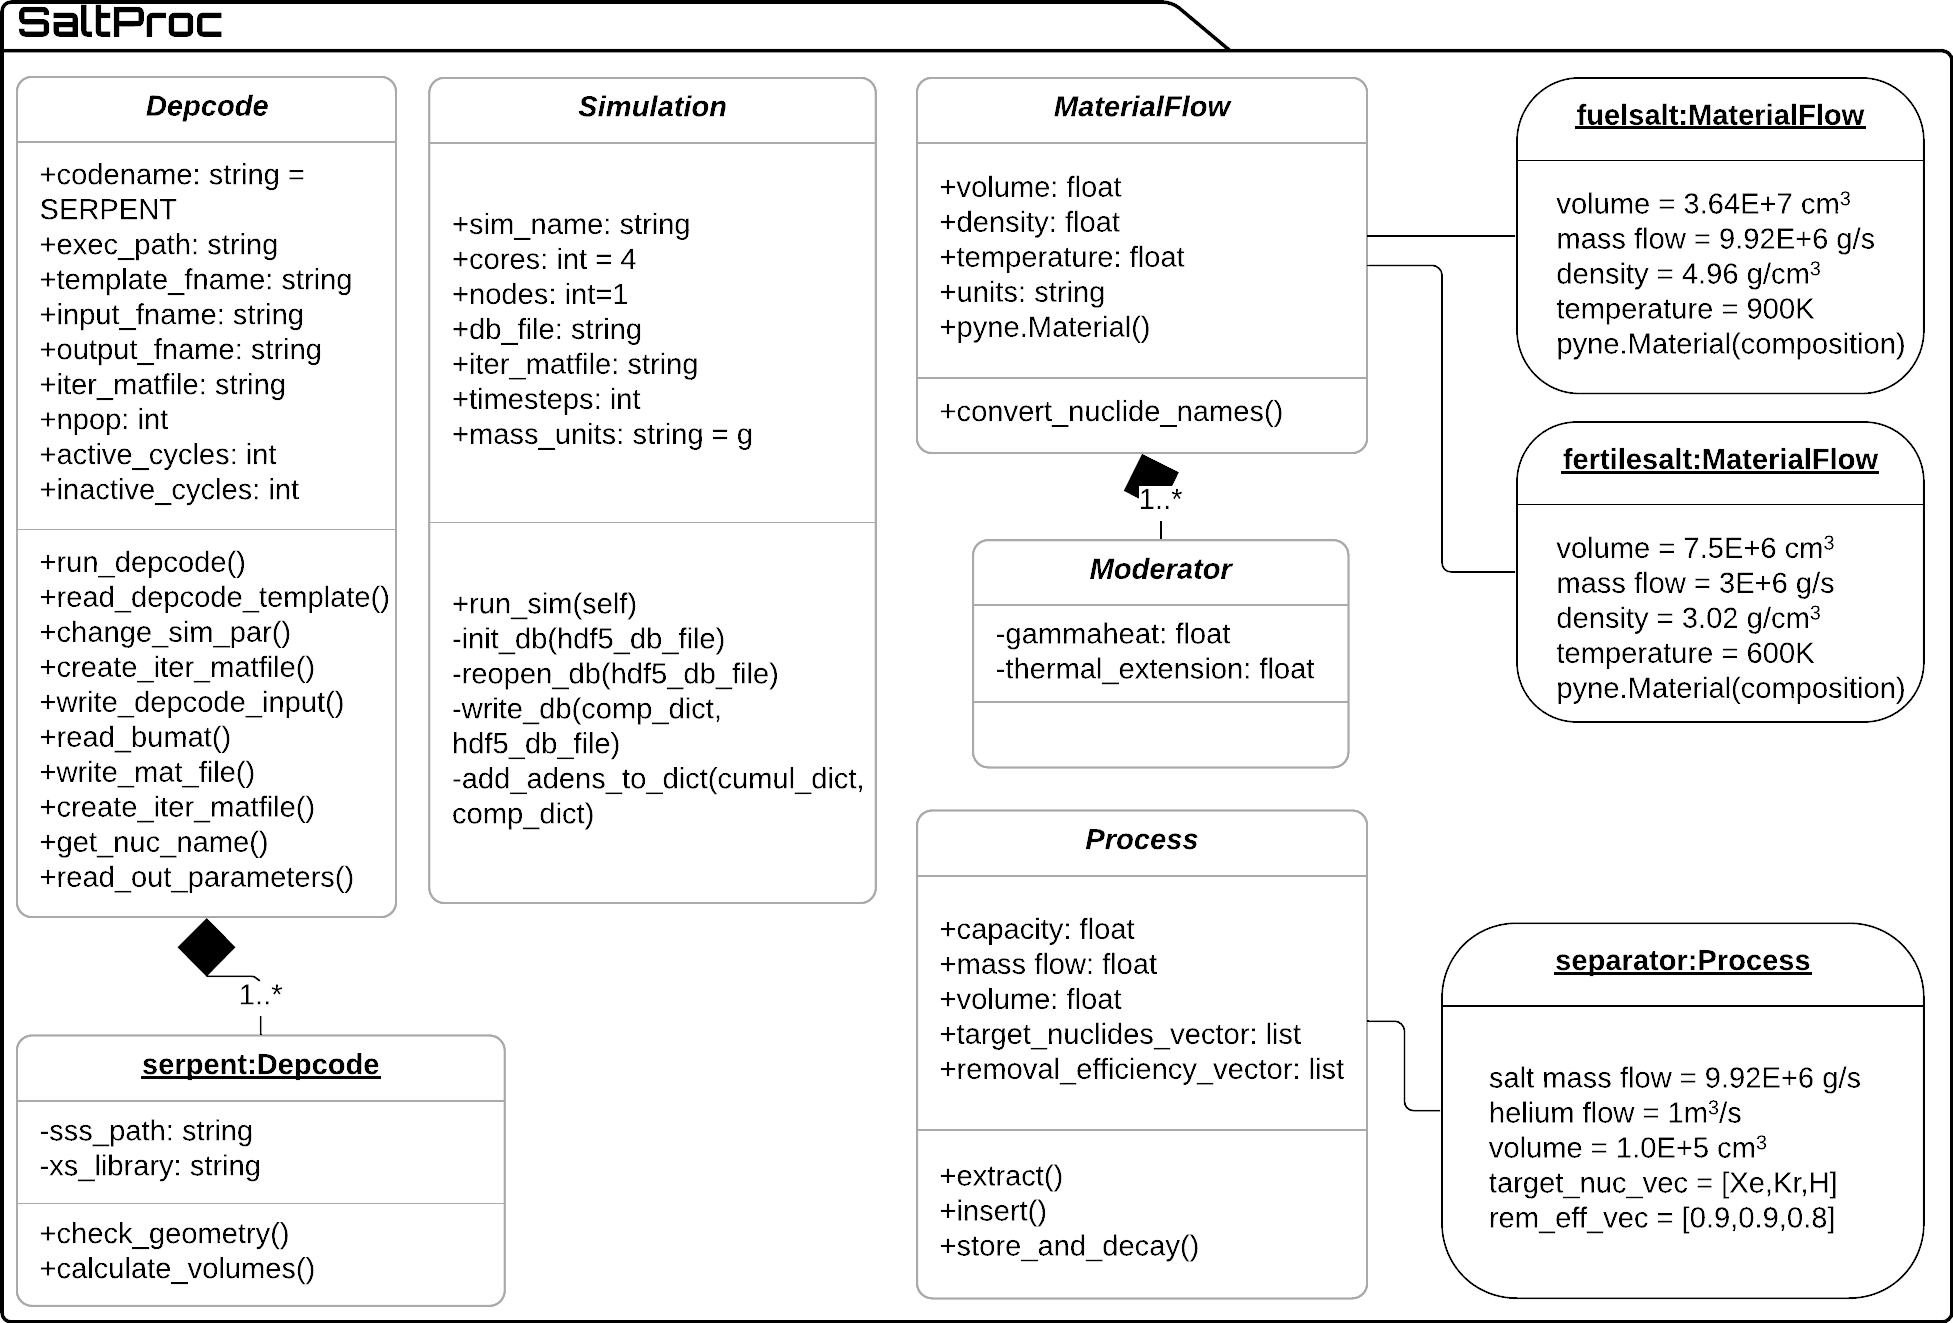
\includegraphics[width=1.01\textwidth]{ch2/saltproc_class_diagram.png}
	\vspace{-0.15in}
	\caption{SaltProc v1.0 python package class diagram in UML 
	notation with examples of object instances.}
	\label{fig:saltproc_class}
\end{figure}
\paragraph{Depcode.}\textit{Depcode} class contains attributes and methods for 
reading the user's input file for the depletion software, initial material 
(e.g., fuel and/or fertile salt) composition, principal parameters for burnup 
simulation (e.g., neutron population and number of cycles for Monte Carlo 
neutron transport), and running the depletion code.
\paragraph{Simulation.}\textit{Simulation} class runs Serpent depletion step, 
creates and writes HDF5 database, tracks time and converts isotopic 
composition vector nuclide names from Serpent to human-readable format.
\paragraph{MaterialFlow.}Each \textit{MaterialFlow} object represents the 
material flowing between \textit{Process} objects  
(figure~\ref{fig:matflow_obj}). All instances of this class 
contain an isotopic composition vector stored in PyNE Material object, mass 
flow rate, temperature, density, volume, and void fraction. Existing PyNE 
Material capabilities convert the units of the isotopic composition vector 
(e.g., from the atomic density provided by Serpent to a mass fraction or 
absolute mass in desired units) and decay the material (i.e., model the 
\gls{MSBR} protactinium decay tank). The main idea of the 
\textit{MaterialFlow} object is to pass detailed information about the salt 
starting at the \gls{MSR} vessel outlet throughout reprocessing components 
(\textit{Processes}), which modify the \textit{MaterialFlow} object before 
depleting the material in the next Serpent burnup step. 
\begin{figure}[ht!] % replace 't' with 'b' to 
	\centering
	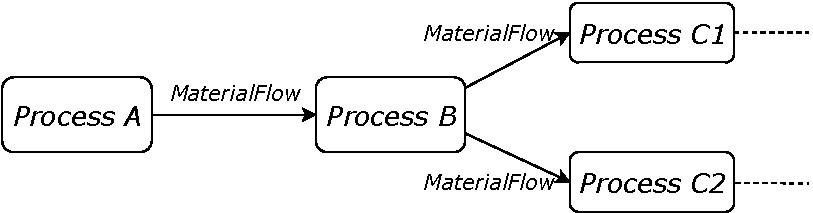
\includegraphics[width=0.7\textwidth]{ch2/materialflow.pdf}
	\vspace{-0.1in}
	\caption{Schematic for passing material data between fuel processing 
		system components.}
	\label{fig:matflow_obj}
\end{figure}
\paragraph{Process.}Each \textit{Process} object represents a 
realistic fuel processing step characterized by its throughput rate, 
volumetric capacity, extraction efficiency for each target element (can be 
a function of many parameters), waste streams, and other process-specific 
parameters. Feed \textit{Process} injects fresh fuel salt 
\textit{MaterialFlow} directly into the reactor core (e.g., adding fissile 
material with a specific mass flow rate to \textit{MaterialFlow} after 
performing all removals).\\


Such a class structure provides outstanding flexibility in simulating 
various \gls{MSR} fuel processing system designs. I created a library of 
various \textit{MaterialFlow} (e.g., fuel salt flow, fertile salt flow, 
refueling salt flow) and \textit{Process} (e.g., helium sparging facility, gas 
separator, nickel filter) objects examples to help a user to 
quickly create a model of a desired reprocessing scheme. At runtime, the user
should connect \textit{Process} objects in series, parallel or both with 
\textit{MaterialFlow} objects to form a comprehensive reprocessing system. To 
make the reprocessing system definition simple and self-explanatory, I 
employed standardized graph description language, \emph{dot}, which is widely 
used in Computer Science \cite{koutsofios_drawing_1996}. The reprocessing 
plant structure described with \emph{dot} can be simply plotted using Graphviz 
\cite{ellson_graphviz_2003} and those plots can be used for analysis, 
optimization, and publications purposes. The user also had flexibility to 
create custom objects with desired attributes and methods and contribute back 
to the code package using GitHub (https://github.com/arfc/saltproc).	

\subsection{Tool flowchart}
Figure~\ref{fig:saltproc_flow} illustrates the online reprocessing simulation 
algorithm coupling SaltProc v1.0 and Serpent. A \emph{json}-compatible 
user input file for SaltProc contains parameters such as paths to depletion 
software executable, neutron population and number of criticality cycles, 
depletion history, total heating power, and list of files with the core 
geometry definition. To perform a depletion step, SaltProc v1.0 reads a 
user-defined Serpent template file. This file contains input parameters such 
as path to nuclear data library, material isotopic composition at startup, 
burnup calculation parameters, and boundary conditions. SaltProc v1.0 
fills in 
the template file and runs Serpent single-step depletion. 

After the depletion calculation, SaltProc v1.0 reads the depleted fuel 
composition file into the \textit{MaterialFlow} object 
(\textit{core\textunderscore outlet} in figure~\ref{fig:saltproc_flow}). This 
object contains an isotopic composition vector, total volume of material, 
total mass, mass flow rate, density, temperature, void fraction, etc. For the 
simplest reprocessing case, when all fuel processing components are located 
in-line (100\% of total material flow goes through a chain of separation 
components), the \textit{core\textunderscore outlet} object is flowing 
sequentially between \textit{Processes} and each \textit{Process} is removing 
a mass fraction of target elements with specified extraction efficiency. 
Afterward, the removed material mass is compensated by fresh fuel salt to 
maintain the salt inventory in a primary loop. Finally, resulting isotopic 
composition after reprocessing is stored in HDF5 database and dumped in a new 
composition file for the next Serpent depletion run. SaltProc v1.0 also 
stores 
isotopic composition before reprocessing and waste stream from each fuel 
processing component in HDF5 database. 
\begin{figure}[ht!] % replace 't' with 'b' to \centering
	\centering
	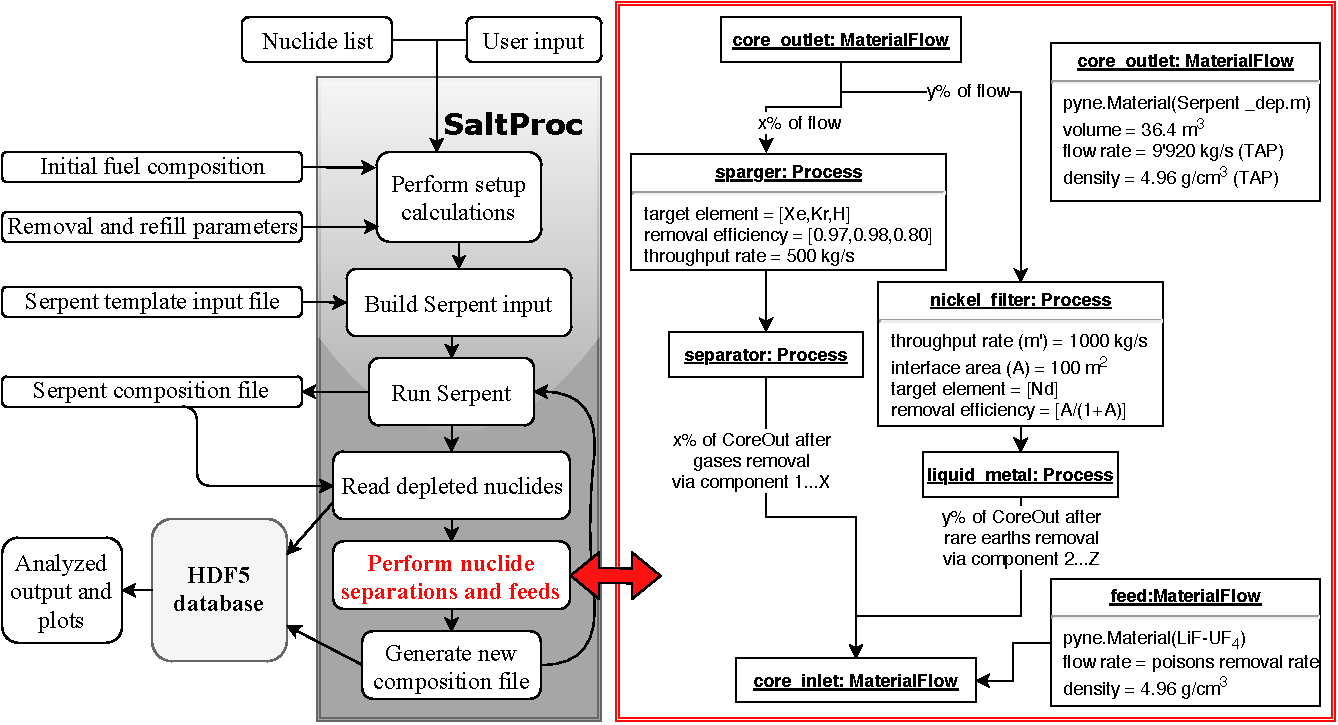
\includegraphics[width=1.01\textwidth]{ch2/saltproc_flowchart.pdf}
	\vspace{-0.15in}
	\caption{Flow chart for SaltProc v1.0 python package.}
	\label{fig:saltproc_flow}
\end{figure}

For a more general case with multiple concurrent extraction processes, a 
separate \textit{MaterialFlow} object is created for each branch with a 
user-defined mass flow rate (e.g., 90\% of total mass flow rate flows via left 
branch and 10\% throughout a right branch). The total mass and isotopic 
composition vector for each \textit{MaterialFlow} object is calculated as a 
fraction of incoming \textit{core\textunderscore outlet} flow. Then each 
\textit{MaterialFlow} object is passed via a cascade of \textit{Processes} to 
separate selected chemical elements with specific efficiency. Finally, the 
left-hand-side branch \textit{MaterialFlow} object is merged with the 
right-hand-side and similarly to the previous case, fresh fuel salt feed 
compensate the loss of mass in separation facilities and keep fuel salt mass 
in a primary loop constant.

The class diagram (Figure~\ref{fig:saltproc_class}) allows to model the 
operation of a complex, multi-zone, multi-fluid \gls{MSR} and is sufficiently 
general to represent myriad reactor systems. SaltProc v1.0 only stores and 
edit the isotopic composition of the fuel stream, which makes it a flexible 
tool to model any geometry: an infinite medium, a unit cell, a multi-zone 
simplified assembly, or a full-core. This flexibility allows the user to 
perform simulations of varying fidelity and computational intensity. 
SaltProc v1.0 is an open-source tool (but a user needs Serpent 2.1.31 
installed to use SaltProc v1.0), available on GitHub. It leverages unit and 
continuous tests crucial for sustainable development \cite{krekel_pytest_2004, 
travis_travis-ci/travis-api_2016}. The documentation is automatically 
generated using Sphinx \cite{brandl_sphinx_2009} and can be found here: 
\emph{https://arfc.github.io/saltproc/}. In summary, the development approach 
of SaltProc v1.0 is focused on producing a generic, flexible and expandable 
tool to give the Serpent 2 Monte Carlo code the ability to conduct advanced 
in-reactor fuel cycle analysis as well as simulate many online refueling and 
fuel reprocessing systems.

\subsection{Reactivity control module}
Simulation of specific \gls{MSR} concepts require to change the reactor core 
geometry during lifetime-long operation modeling. For instance, the \gls{TAP} 
concept aims to increase the core lifetime by using continuous fresh fuel 
feeds, removal of \glspl{FP}, and configurable moderator rod assemblies to 
compensate negative reactivity insertion due to fissile material burnup. The 
concept proposes to maintaining reactivity in the long term by replacing 
stationary moderator assemblies with more highly populated lattices to 
increase the moderator-to-fuel ratio \cite{betzler_assessment_2017-1}. 
SaltProc v1.0 is able to switch from one file containing the core geometry to 
another core geometry (e.g., with larger moderator-to-fuel ratio) if effective 
multiplication factor, $k_{eff}$, falls below a specific limit (e.g., 1.002). 
This very unique capability allows SaltProc v1.0 analyze fuel cycle 
performance of any liquid-fueled \gls{MSR} system, including advanced designs 
with moving moderator.

%\section{Multi-component fuel salt reprocessing system}
\section{Concluding remarks}
In this Chapter, the overview of fuel salt reprocessing plant has first been 
presented. I described various components of the plant and the physical or 
chemical mechanism responsible for neutron poisons extraction from the salt. 
General core physics aspects and Serpent 2 depletion software capabilities 
have then been discussed. I also introduced SaltProc, the Python package 
developed and used to simulate continuous feeds and removals in various 
\gls{MSR} designs.

In the following chapters, SaltProc v1.0 will be demonstrated and validated 
for a two liquid-fueled \gls{MSR} designs.
\chapter{Tool demonstration for lifetime-long depletion: Molten Salt Breeder 
Reactor}

This chapter describes the fuel cycle analysis of the \gls{MSBR} obtained 
using the open-source Python package, SaltProc. The development was initially 
started as a part of my master thesis \cite{rykhlevskii_advanced_2018} in 
2017. This effort, for verification purposes, assumed ideal extraction 
efficiency (e.g., 100\% of the target isotope mass extracted) because all 
results available in the literature also rely on this assumption.

The main results presented in this chapter have been published in: A. 
Rykhlevskii, J.W. Bae, and K. D. Huff, ``Modeling and simulation of online 
reprocessing in the thorium-fueled molten salt breeder reactor,'' 
\textit{Annals of Nuclear Energy}, 128 (2019): 366--379. The high-fidelity, 
full-core \gls{MSBR} model has been presented at the 2017 \gls{ANS} Winter 
Meeting in Washington, D.C. The fuel salt composition evolution has been 
presented at the 2018 Blue Waters Symposium in Sunriver, OR 
\cite{rykhlevskii_computational_2018-1}. The obtained results relevant to 
\gls{MSBR} analysis have been compared against those obtained by Benjamin R. 
Betzler and colleagues for a simplified unit cell model, adopting the in-house 
code ChemTriton \cite{betzler_molten_2017}. 


\section{Introduction}
The thorium-fueled \gls{MSBR} was developed in the early 1970s by \gls{ORNL},  
specifically to explore the promise of the thorium fuel cycle, which uses 
natural fertile thorium feed material instead of enriched uranium fissile 
fuel. With continuous fuel reprocessing, the \gls{MSBR} realizes the 
advantages of the thorium fuel cycle because the $^{233}$U bred from 
$^{232}$Th is almost instantly\footnote{\space The fertile $^{232}$Th is 
transmuted into the $^{233}$Th after capturing a neutron. Next, this isotope 
decays to the $^{233}$Pa ($\tau_{1/2}$=21.83m), which finally decays to the 
$^{233}$U ($\tau_{1/2}$=26.967d).} recycled back into the core  
\cite{betzler_modeling_2016}. The chosen fuel salt, 
LiF-BeF$_2$-ThF$_4$-UF$_4$, has a melting point of $499^\circ$C, low vapor 
pressure at operating temperatures, and beneficial flow and heat transfer 
properties \cite{robertson_conceptual_1971}. 

In this work, we analyzed the \gls{MSBR} neutronics and fuel cycle to  
establish its equilibrium core composition. Additionally, we compared  
predicted operational and safety parameters of the \gls{MSBR} at both the  
initial and equilibrium states to characterize the evolution of its safety 
case over time. Moreover, these depletion simulations determined the  
appropriate $^{232}$Th feed rate for maintaining criticality and enabled 
analysis of the overall \gls{MSBR} fuel cycle performance. Finally, the 
benefits of online fission product removal in the thermal spectrum \gls{MSBR} 
were identified.


\section{Molten Salt Breeder Reactor design and model description}
Figure~\ref{fig:msbr_elev_view} shows the \gls{MSBR} vessel which has a 
diameter of 680 cm and
a height of 610 cm. It contains a molten fluoride 
fuel-salt mixture that generates heat in the active core region and transports 
that heat to the primary heat exchanger by way of the primary salt pump. In 
the active core region, the fuel salt flows through channels in moderating and 
reflecting graphite blocks. Fuel salt at 565$^{\circ}$C enters the central 
manifold at the bottom via four 40.64-cm-diameter nozzles and flows upward 
through channels in the lower plenum graphite. The fuel salt exits at the top 
at about 704$^{\circ}$C through four equally spaced nozzles, which connect to 
the salt-suction pipes leading to primary circulation pumps. The fuel salt 
drain lines connect to the bottom of the reactor vessel inlet manifold.
\begin{figure}[ht!] % replace 't' with 'b' to \centering
	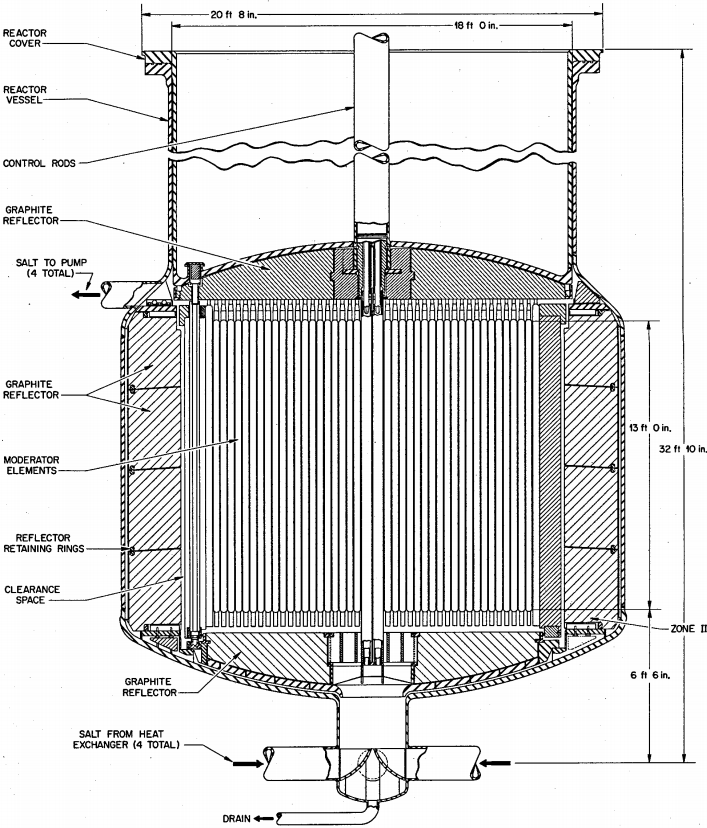
\includegraphics[width=\textwidth]{ch3/msbr_elev_view.png}
	\caption{$XZ$ view of the \gls{MSBR} (reproduced from Robertson \emph{et 
	al.} \cite{robertson_conceptual_1971}).}
	\label{fig:msbr_elev_view}
\end{figure}

Figure~\ref{fig:serpent_plan_view} shows the configuration of the \gls{MSBR} 
vessel, including the ``fission" (zone I) and ``breeding" (zone II) regions 
inside the vessel. The core has two radial zones bounded by a solid  
cylindrical graphite reflector and the vessel wall. The central zone, zone I, 
in which 13\% of the volume is fuel salt and 87\% is graphite, is composed of 
1,320 graphite cells, 2 graphite control rods, and 2 emergency shutdown rods. 
The under-moderated zone, zone II, in which 37\% of the volume is fuel salt 
and 63\% is graphite, and radial reflector, surrounds the zone I core region 
and serves to diminish neutron leakage. Zones I and II are surrounded radially 
and axially by fuel salt (Figure~\ref{fig:serpent_zoneII}); this space for 
fuel is necessary for the injection and flow of molten salt.
\begin{figure}[htb!] % replace 't' with 'b' to \centering
	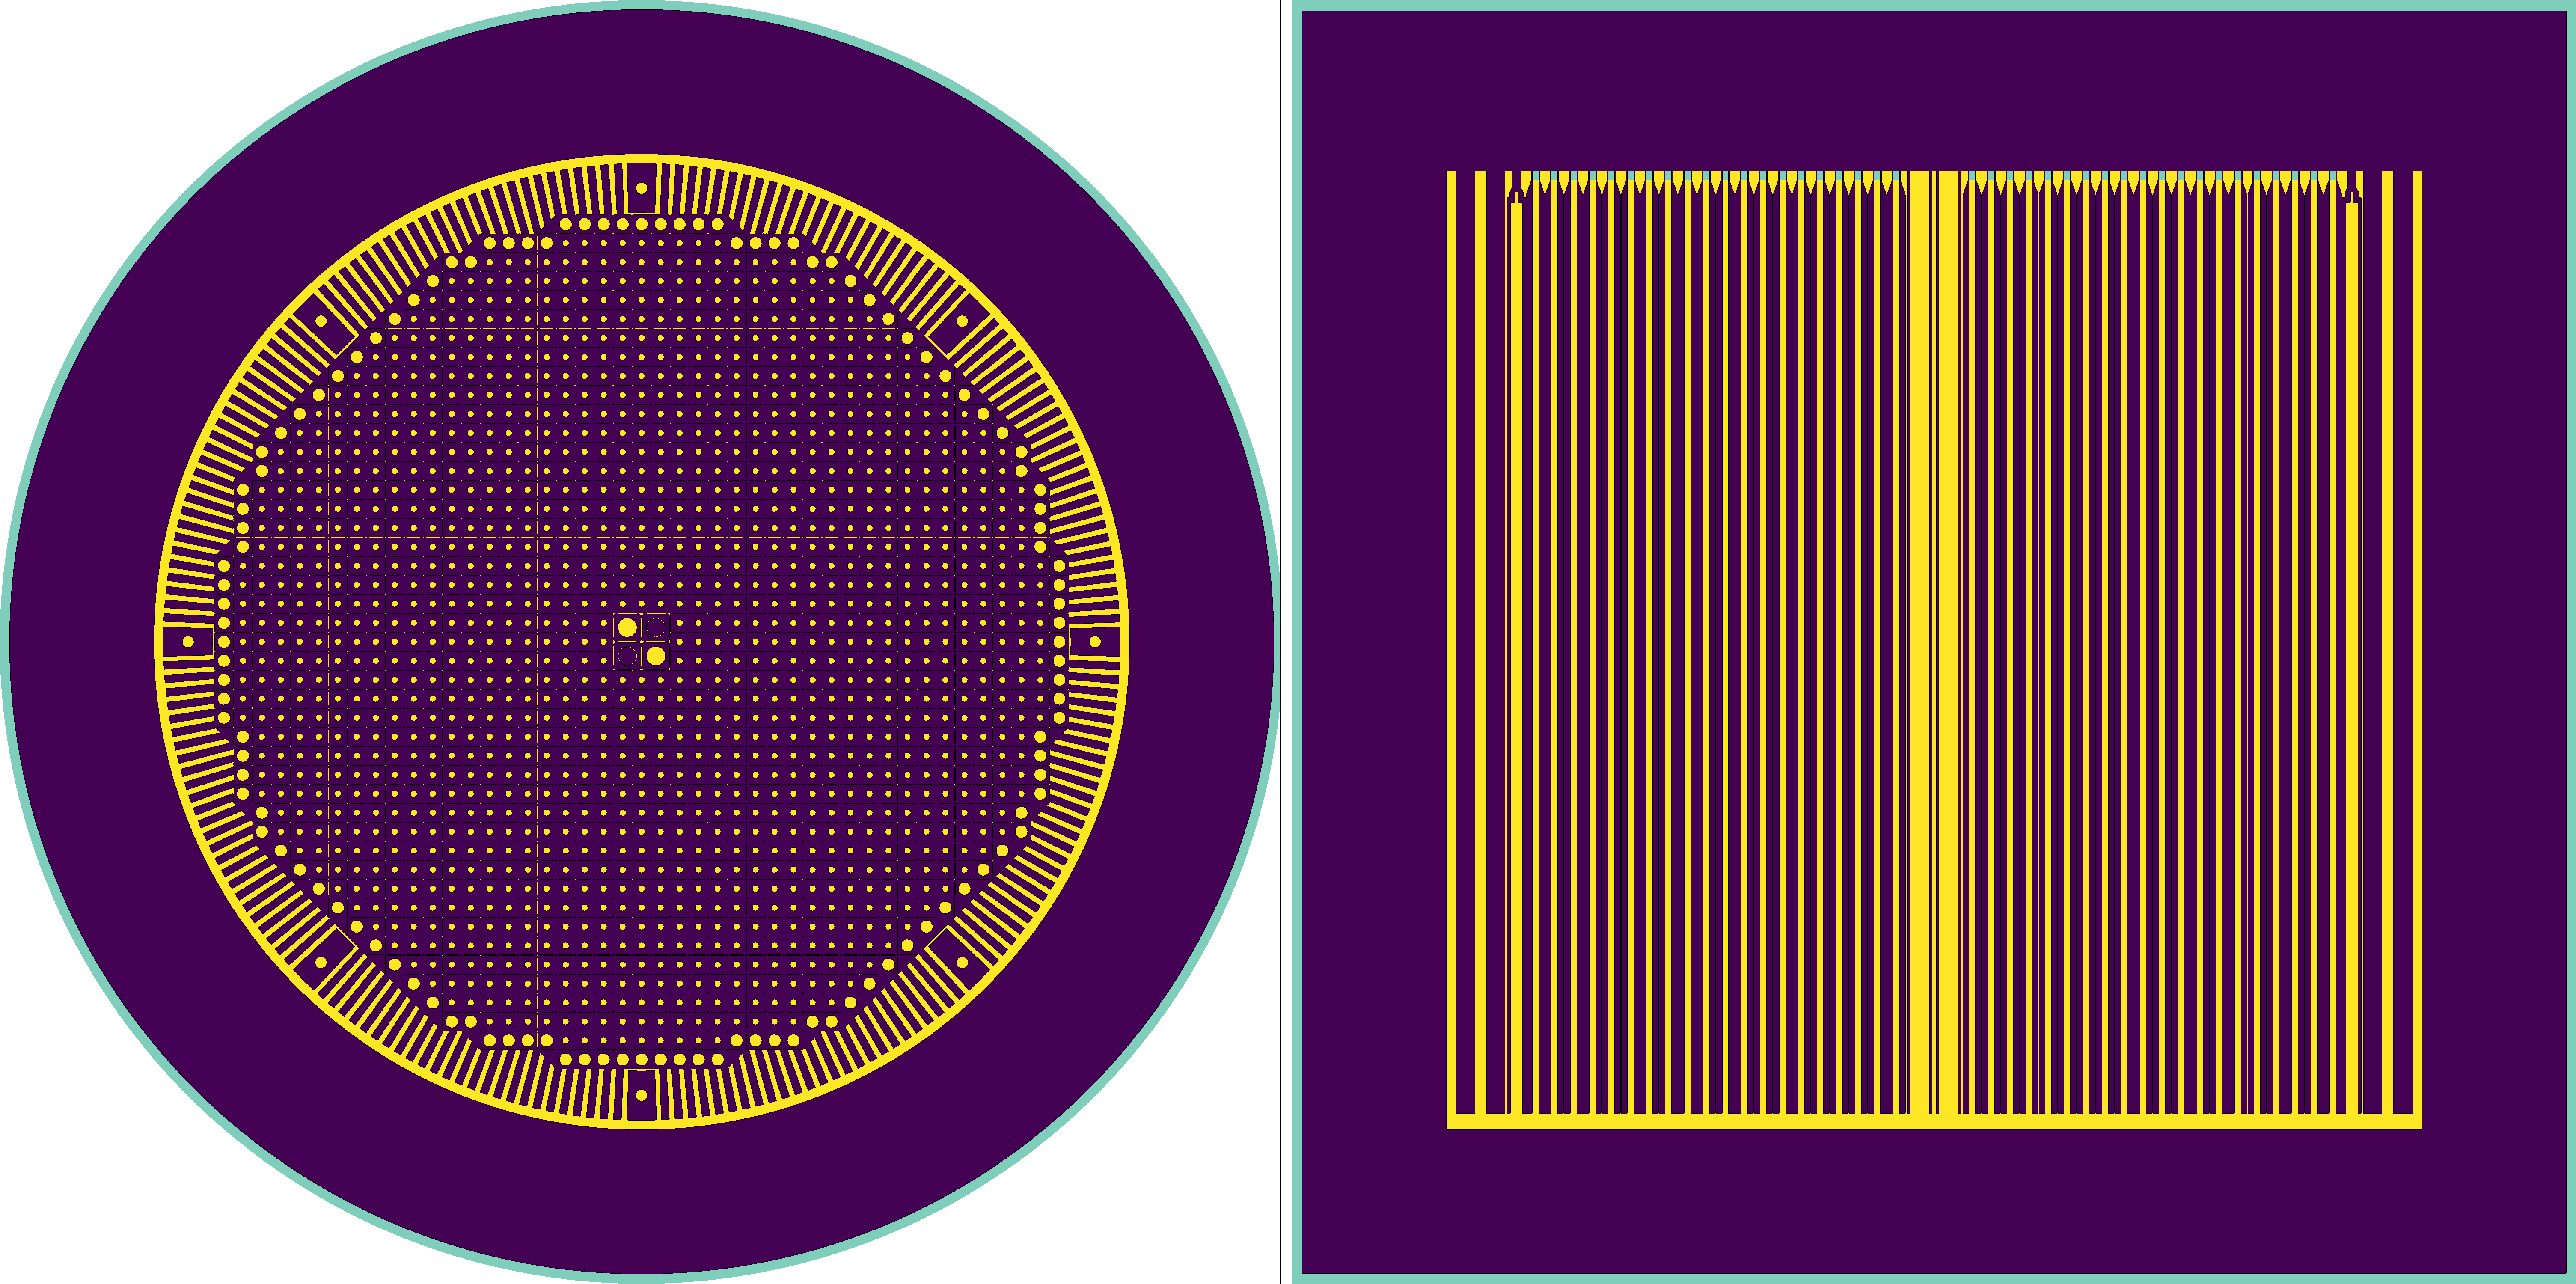
\includegraphics[width=\textwidth]{ch3/view_serpent.png}
	\caption{$XY$ (left) and $XZ$ (right) views of a Serpent \gls{MSBR} model
	(reproduced from Rykhlevskii \emph{et al.} 
	\cite{rykhlevskii_modeling_2019}).}
	\label{fig:serpent_plan_view}
\end{figure}

\begin{figure}[htb!] % replace 't' with 'b' to \centering
	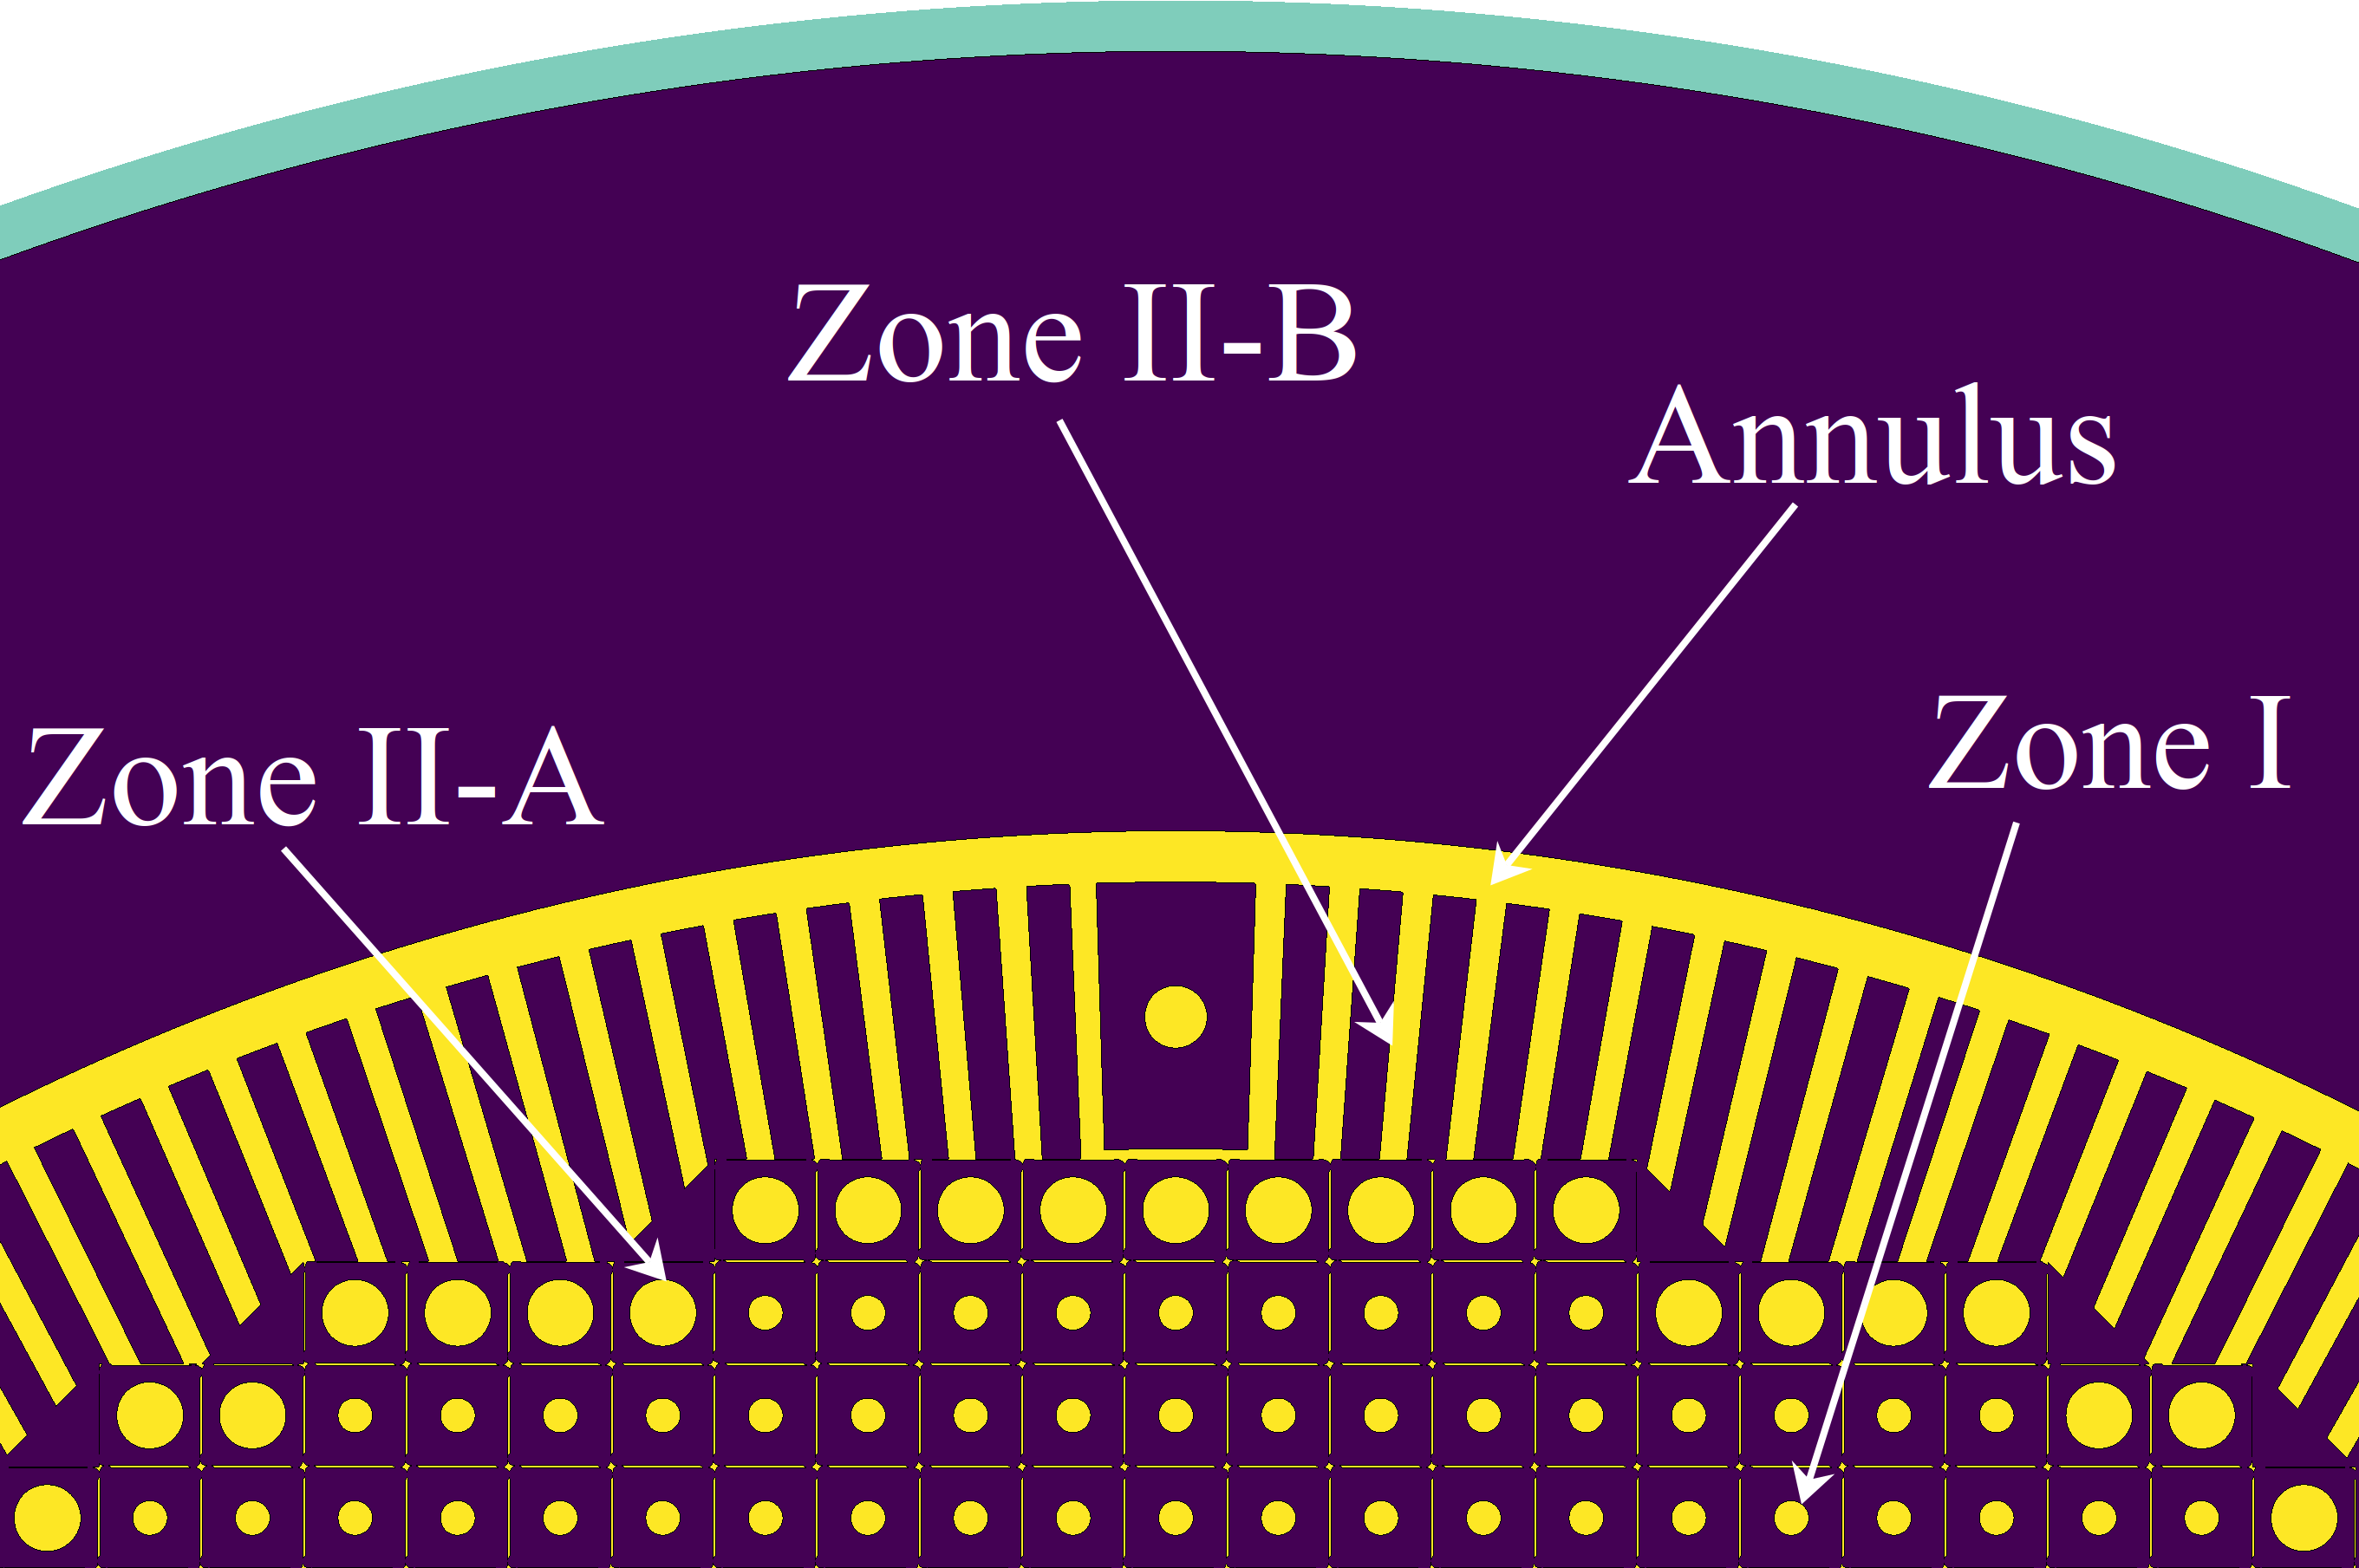
\includegraphics[width=\textwidth]{ch3/ser_zone_II.png}
	\caption{Detailed view of the \gls{MSBR} two-zone model. 
		Yellow represents fuel salt, purple represents graphite, and aqua 
		represents the reactor vessel (reproduced from Rykhlevskii 
		\emph{et al.} \cite{rykhlevskii_modeling_2019}).}
	\label{fig:serpent_zoneII}
\end{figure}

Since reactor graphite experiences significant dimensional changes due to 
neutron irradiation, the reactor core was designed for periodic replacement. 
Based on the experimental irradiation data from the \gls{MSRE}, the core 
graphite lifetime is about 4 years, and the reflector graphite lifetime is 30 
years \cite{robertson_conceptual_1971}.

The core design also has eight symmetric graphite slabs with a width of 15.24 
cm in zone II, one of which is illustrated in Figure~\ref{fig:serpent_zoneII}. 
The holes in the centers are for the core lifting rods used during the core 
replacement operations. These holes also allow a portion of the fuel salt to 
flow to the top of the vessel for cooling the top head and axial reflector.  
Figure~\ref{fig:serpent_zoneII} also shows the 5.08-cm-wide annular 
space between the removable core graphite in zone II-B and the permanently 
mounted reflector graphite. This annulus consists entirely of fuel salt, 
provides space for moving the core assembly, helps compensate for the 
elliptical dimensions of the reactor vessel, and serves to reduce the damaging 
flux at the surface of the graphite reflector blocks. 

$^{135}$Xe is a strong neutron poison, and some fraction of this gas is  
absorbed by graphite during \gls{MSBR} operation. ORNL calculations showed 
that for unsealed commercial graphite with a helium permeability of 10$^{-5}$ 
cm$^2$/s, the calculated $^{135}$Xe poison fraction\footnote{The original ORNL 
report by Robertson \emph{et al.} defined $^{135}$Xe poison fraction as the 
number of neutrons absorbed by $^{135}$Xe compared with the total number of 
neutrons (both fast and thermal) absorbed by $^{233}$U.} is less than 2\%
\cite{robertson_conceptual_1971}. This parameter can be improved by using 
experimental graphite types or by applying sealing technology. The effect of 
the gradual poisoning of the core graphite with xenon is outside of the scope 
of this work.

\subsection{Core zone I}
The central region of the core, called zone I, is made up of graphite 
elements, each $10.16$cm$\times$ 10.16cm$\times$396.24cm and has 13\% fuel 
salt by volume. Zone I has 4 
channels for control rods: two for graphite rods, which both regulate and shim 
during normal operation, and two for backup safety rods consisting of boron 
carbide clad to assure sufficient negative reactivity for accidents.

Zone I graphite elements have a mostly rectangular shape with lengthwise 
ridges at each corner that leave space for salt flow around the elements. 
Figure~\ref{fig:I_element_ref} shows the 
elevation and plan views of graphite elements of zone I 
\cite{robertson_conceptual_1971} and their Serpent model 
\cite{rykhlevskii_full-core_2017}.
\begin{figure}[ht!] % replace 't' with 'b' to \centering
	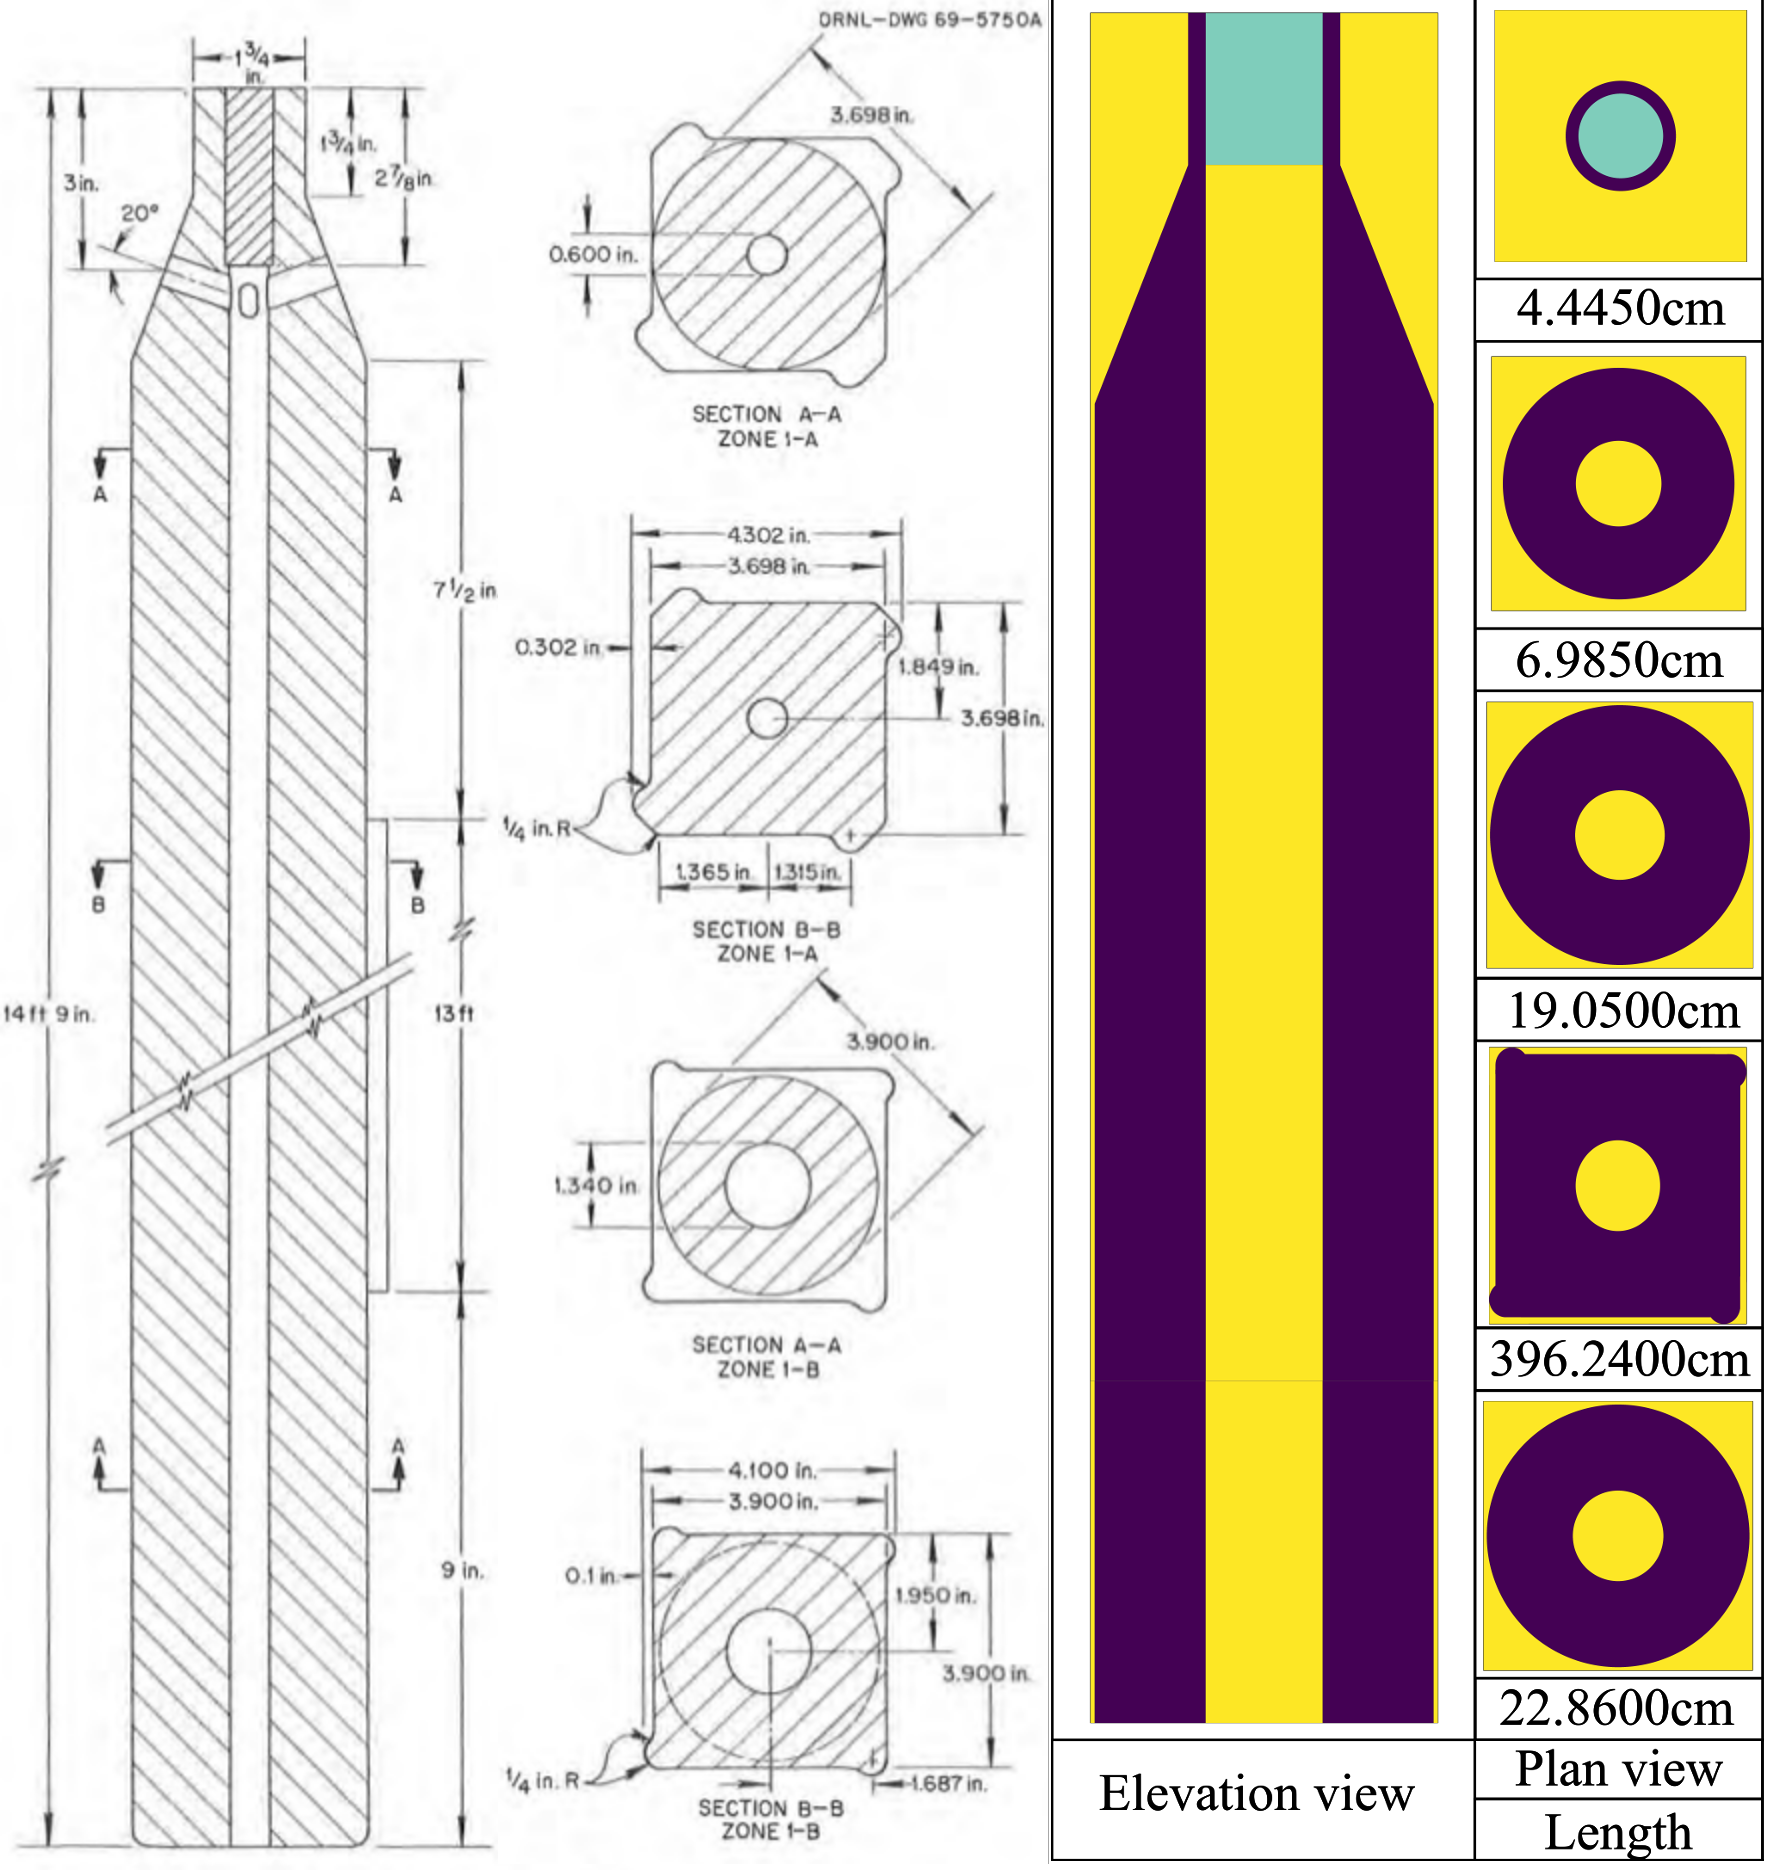
\includegraphics[width=\textwidth]{ch3/zone_I_element_ref.png}
	\caption{Graphite moderator elements for zone I: reference design (left)
		\cite{robertson_conceptual_1971} and Serpent model (right) 
		\cite{rykhlevskii_full-core_2017}.  Yellow 
		represents fuel salt, purple represents graphite, and aqua represents 
		the reactor vessel (reproduced from Rykhlevskii \emph{et al.} 
		\cite{rykhlevskii_modeling_2019}).}
	\label{fig:I_element_ref}
\end{figure}

\subsection{Core zone II}
Zone II, which is undermoderated, surrounds zone I. Combined with the bounding 
radial reflector, zone II serves to diminish neutron leakage. Two kinds of 
elements form this zone: large-diameter fuel channels (zone II-A) and 
radial graphite slats (zone II-B). 

Zone II has 37\% fuel salt by volume, and each element has a fuel channel 
diameter of 6.604cm. The graphite elements for zone II-A are prismatic, with
elliptical dowels running axially between the prisms. These dowels
isolate the fuel salt flow in zone I from that in zone II.  
Figure~\ref{fig:II_element_ref} shows the shapes and dimensions of these 
graphite elements and their Serpent model. Zone II-B elements are rectangular 
slats spaced far enough apart to provide the 0.37 fuel salt volume fraction. 
The reactor zone II-B graphite 5.08cm-thick slats vary in the radial dimension 
(average width is 26.67cm) as shown in Figure~\ref{fig:serpent_zoneII}. Zone 
II serves as a blanket to achieve the best performance: a high breeding ratio 
and a low fissile inventory. The harder neutron energy spectrum in zone II 
enhances the rate of thorium resonance capture relative to the fission rate, 
thus limiting the neutron flux in the outer core zone and reducing the neutron 
leakage \cite{robertson_conceptual_1971}. 

The sophisticated, irregular shapes of the fuel elements challenge an accurate 
representation of zone II-B. The suggested design 
\cite{robertson_conceptual_1971} of zone II-B has eight irregularly-shaped 
graphite elements as well as dozens of salt channels. These graphite elements 
were simplified into right-circular cylindrical shapes with central channels. 
Figure~\ref{fig:serpent_zoneII} illustrates this core region in the Serpent 
model. The volume of fuel salt in zone II was kept exactly at 37\% so 
this simplification did not impact the core neutronics. 
Simplifying the eight edge channels was the only simplification made to the 
\gls{MSBR} geometry in this work. 
\begin{figure}[ht!] % replace 't' with 'b' to \centering
	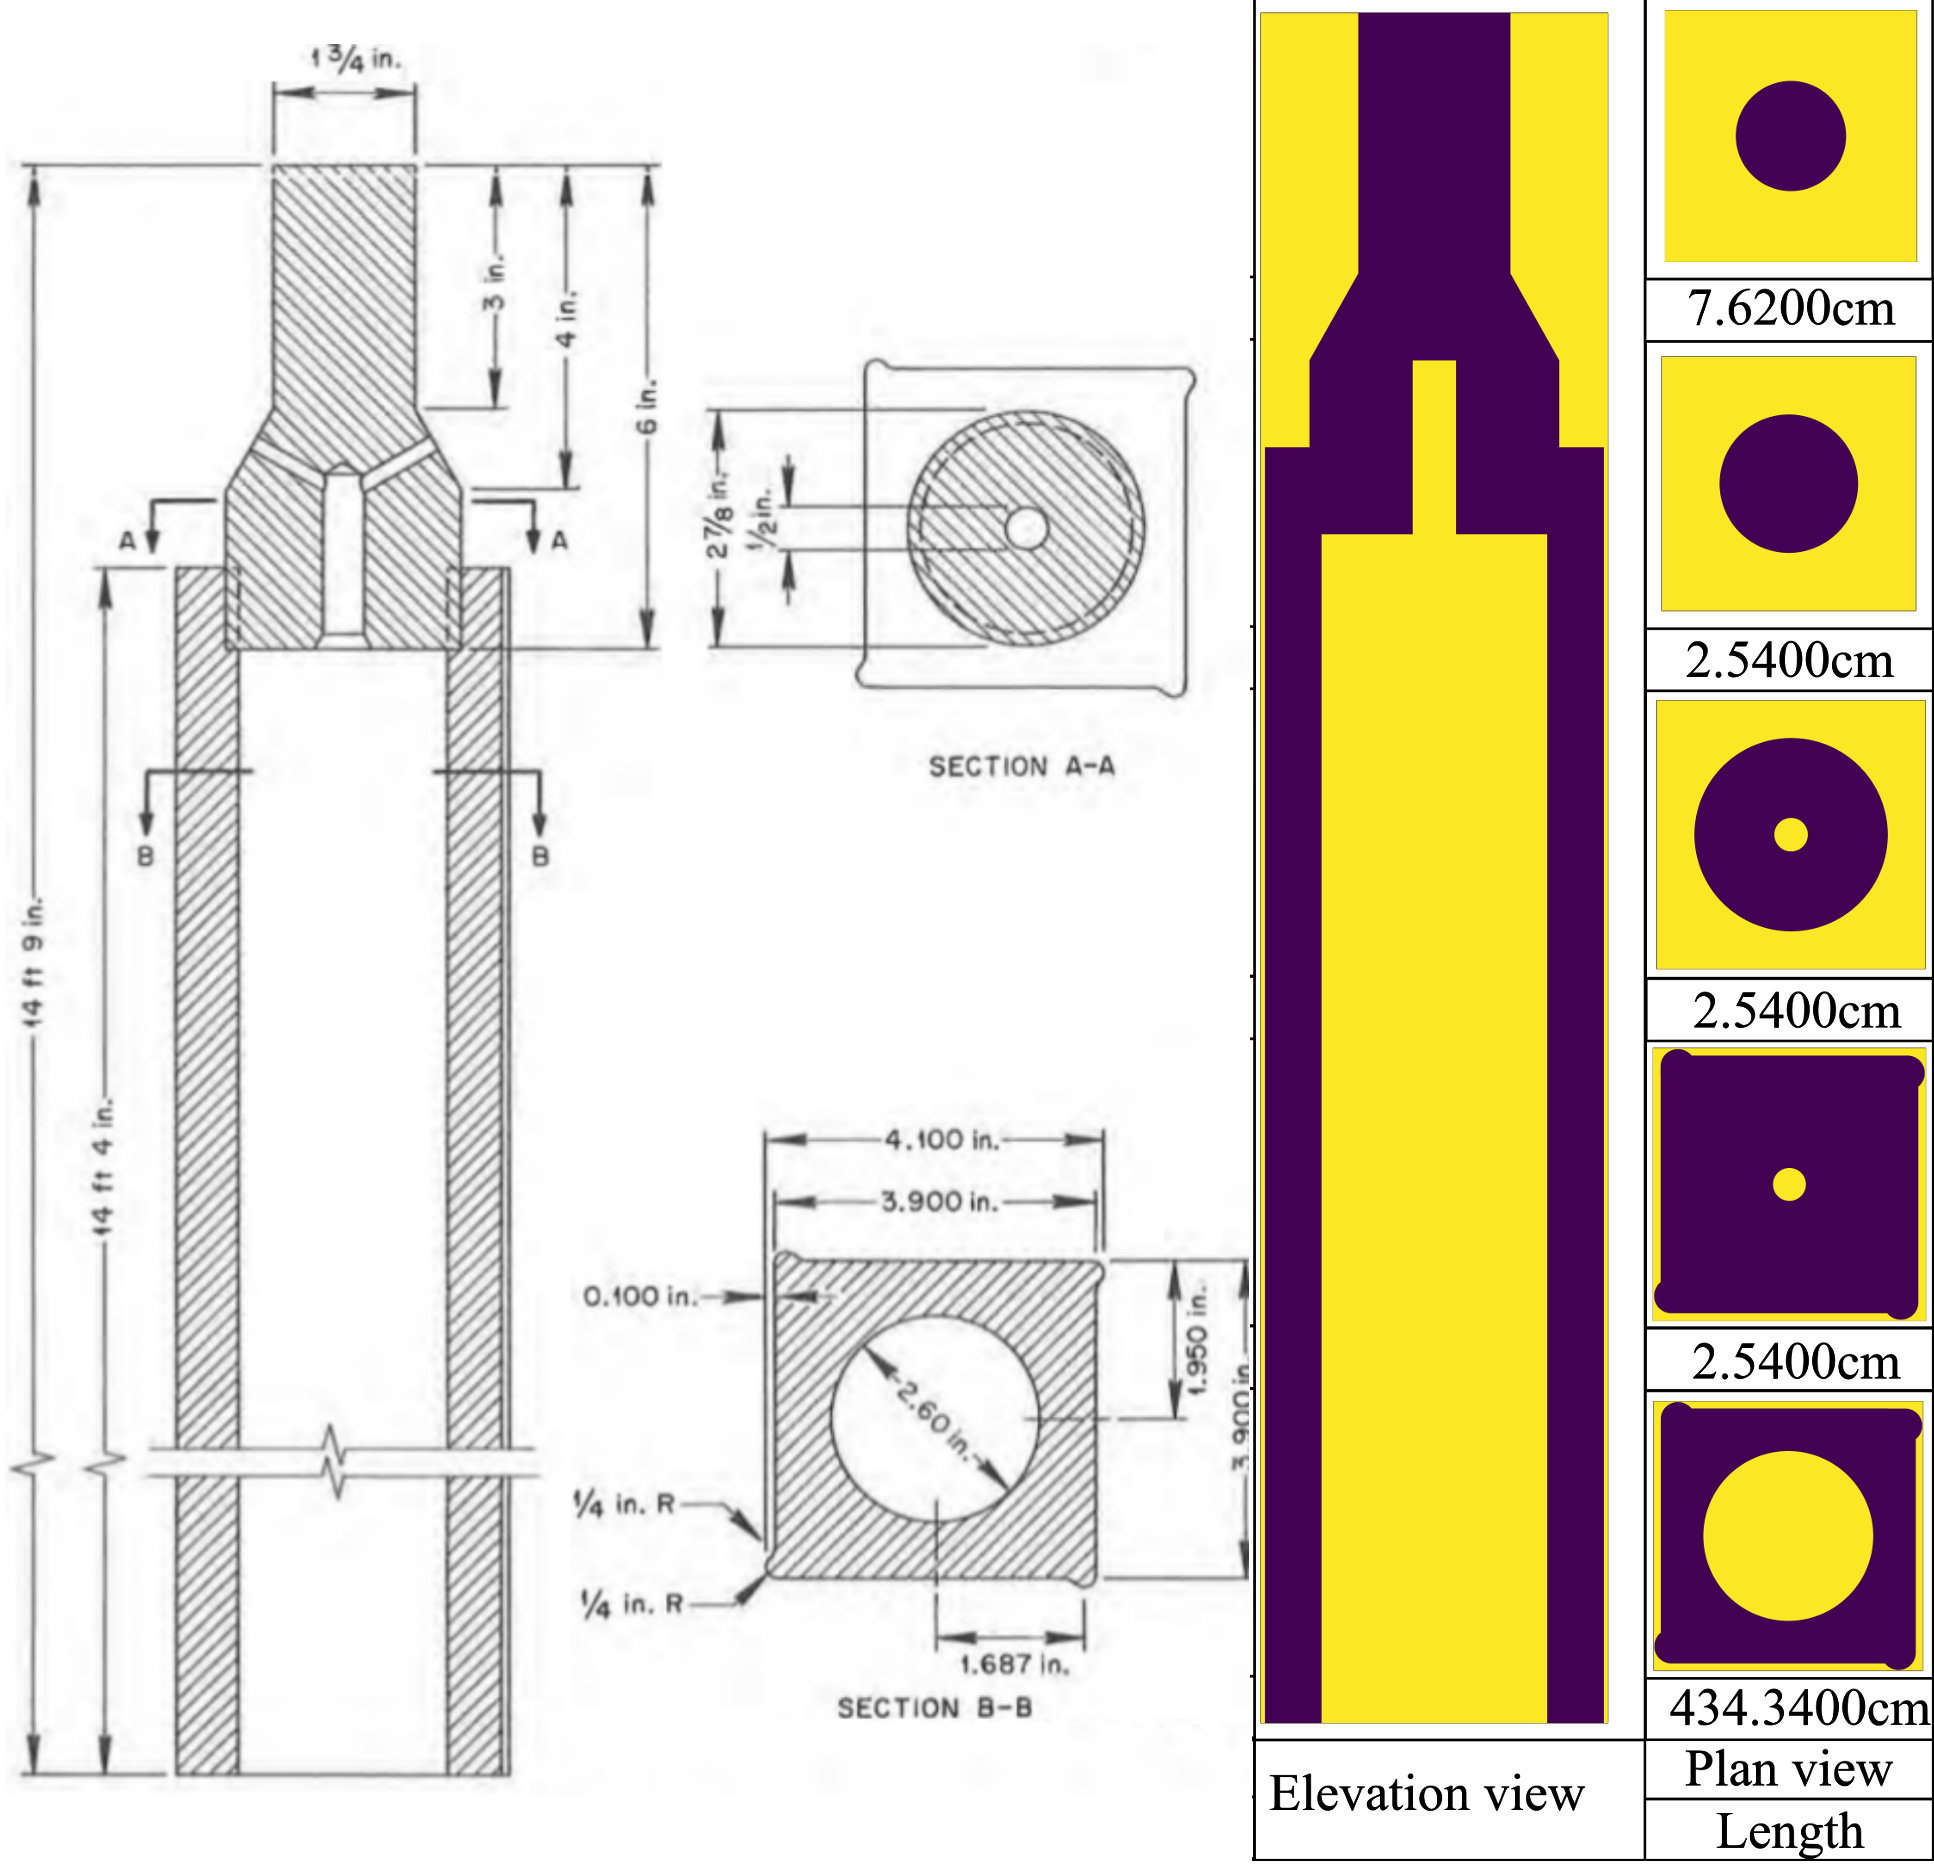
\includegraphics[width=\textwidth]{ch3/zone_II_element_ref.png}
	\caption{Graphite moderator elements for zone II-A: reference design (left)
		\cite{robertson_conceptual_1971} and Serpent model (right) 
		\cite{rykhlevskii_full-core_2017}.  Yellow 
		represents fuel salt, purple represents graphite, and aqua represents 
		the reactor vessel (reproduced from Rykhlevskii \emph{et al.} 
		\cite{rykhlevskii_modeling_2019}).}
	\label{fig:II_element_ref}
\end{figure}

\subsection{Material composition and normalization parameters}
The fuel salt, reactor graphite, and modified Hastelloy-N are all materials 
invented at \gls{ORNL} specifically for the \gls{MSBR}. The fuel salt selected 
for use in the \gls{MSBR} is LiF-BeF$_2$-ThF$_4$-$^{233}$UF$_4$ 
(71.75-16-12-0.25 mole \% which has density of 3.35 g/cm$^3$ 
\cite{robertson_conceptual_1971}. The lithium in the molten salt fuel is fully 
enriched to 99.995\% $^{7}$Li because $^{6}$Li is an extremely strong neutron 
poison and becomes tritium upon neutron capture. 

The specific temperature was fixed for each material and stays constant during 
reactor operation. The isotopic composition of each material at the 
initial state was described in detail in the MSBR conceptual design study 
\cite{robertson_conceptual_1971} and has been applied to the Serpent model 
without any modification. Table~\ref{tab:msbr_tab} is a summary of the major 
\gls{MSBR} parameters used to inform the Serpent model  
\cite{robertson_conceptual_1971}. 
%%%%%%%%%%%%%%%%%%%%%%%%%%%%%%%%%%%%%%%%
\begin{table}[h!]
	\caption{Summary of principal data for the \gls{MSBR} (reproduced from 
	Robertson \emph{et al.} \cite{robertson_conceptual_1971}).}
		\centering
	\begin{tabularx}{0.71\textwidth}{ L  R}
		\hline
		Thermal power           					& 2250 MW$_{th}$\\
		Electric power             					& 1000 MW$_e$   \\
		Gross thermal efficiency       				& 44.4\%        \\
		Salt volume fraction (Zone I)       		& 0.13   		\\
		Salt volume fraction (Zone II)              & 0.37			\\
		Fuel salt inventory (Zone I)                & 8.2 m$^3$		\\
		Fuel salt inventory (Zone II)               & 10.8 m$^3$	\\
		Fuel salt inventory (annulus)               & 3.8 m$^3$		\\
		Total fuel salt inventory                   & 48.7 m$^3$	\\
		Fissile mass in fuel salt                   & 1303.7 kg		\\
		Fuel salt components   	& LiF-BeF$_2$-ThF$_4$-$^{233}$UF$_4$\\  
		Fuel salt composition   & 71.75-16-12-0.25 mole\%			\\
		Fuel salt density       & 3.35 g/cm$^3$         			\\ \hline
	\end{tabularx}
	\label{tab:msbr_tab}
\end{table}
%%%%%%%%%%%%%%%%%%%%%%%%%%%%%%%%%%%%%%%%%%%%%%%%

As mentioned in section~\ref{sec:reproc-plant}, the \gls{MSBR} design 
requires online reprocessing to completely remove neutron gaseous \glspl{FP} 
(Xe, Kr) and noble metals (e.g., Se, Nb, and Mo) every 20 seconds.  The 
$^{232}$Th in the fuel absorbs thermal neutrons and produces $^{233}$Pa, which 
then decays into the fissile $^{233}$U. Protactinium presents a challenge 
since it has a large absorption cross section in the thermal energy spectrum. 
Moreover, $^{233}$Pa left in the core produces $^{234}$Pa and $^{234}$U, 
neither of which are useful as fuel. Accordingly, $^{233}$Pa is continuously 
removed from the fuel salt into a temporary storage tank to allow $^{233}$Pa 
to decay to $^{233}$U without the corresponding negative neutronic impact. The 
reactor chemical processing system must separate $^{233}$Pa from the molten 
salt fuel over 3 days, hold it while $^{233}$Pa decays into $^{233}$U, and 
return it to the primary loop. This feature allows the reactor to avoid 
neutron losses to protactinium, lowers in-core fission product inventory, and 
increases the efficiency of $^{233}$U breeding.

Table~\ref{tab:reprocessing_list_msbr} summarizes a full list of nuclides and 
their cycle time used for modeling salt treatment and separations 
\cite{robertson_conceptual_1971}. The removal rates vary among chemical 
elements in this reactor concept and dictate the necessary resolution of 
depletion calculations. If the depletion time intervals are short, an 
enormous number of depletion steps are required to obtain the equilibrium 
composition. On the other hand, if the depletion calculation time interval is 
too long, effective multiplication factor $k_{eff}$ would be lower than 
expected in reality due to higher equilibrium concentration of strong poisons 
(e.g., $^{135}$Xe) in fuel salt. To compromise, a 3-day time interval was 
selected for depletion calculations to correlate with the removal interval of 
$^{233}$Pa as suggested by Powers \emph{et al.} \cite{powers_new_2013}. 
Finally, $^{232}$Th was continuously added every 3 days to maintain the 
initial mass fraction of $^{232}$Th in the fuel salt.
%%%%%%%%%%%%%%%%%%%%%%%%%%%%%%%%%%%%%%%%
\begin{table}[ht!]
	\caption{The cycle times for protactinium and fission product removal from 
	the \gls{MSBR} (reproduced from Robertson \emph{et al.} 
		\cite{robertson_conceptual_1971}).}
	\begin{tabularx}{\textwidth}{x  s  x}
		\hline \textbf{Processing group} & \qquad\qquad\qquad 
		\textbf{Nuclides} & \textbf{Cycle time (at full power)} \\ \hline 
		Rare earths & Y, La, Ce, Pr, Nd, Pm, Sm, 
		Gd & 50 days \\ \qquad & Eu & 500 days \\ Noble metals & Se, 
		Nb, Mo, Tc, Ru, Rh, Pd, Ag, Sb, Te & 20 sec \\
		Semi-noble metals & Zr, Cd, In, Sn & 200 days \\
		Gases & Kr, Xe & 20 sec \\ Volatile fluorides & Br, I & 60 days \\
		Discard & Rb, Sr, Cs, Ba & 3435 days \\ 
		%Salt discard & Th, Li, Be, F & 3435 days \\ 
		Protactinium & $^{233}$Pa & 3 days \\ Higher 
		nuclides & $^{237}$Np, $^{242}$Pu & 16 years \\  \hline
	\end{tabularx}
	\label{tab:reprocessing_list_msbr}
\end{table}
%%%%%%%%%%%%%%%%%%%%%%%%%%%%%%%%%%%%%%%%%

\section{Fuel salt isotopic composition dynamics and equilibrium search}
\label{sec:equilibrium_search}
The SaltProc online reprocessing simulation package is demonstrated in four 
applications: 
(1) analyzing the \gls{MSBR} neutronics and fuel cycle to find 
the equilibrium core composition and fuel salt depletion, 
(2) demonstrating that in a single-fluid two-region \gls{MSBR} conceptual 
design the undermoderated outer core zone II works as a virtual ``blanket'', 
reduces neutron leakage, and improves breeding ratio due to neutron energy 
spectral shift,
(3) studying operational and safety parameters evolution during \gls{MSBR} 
operation, and
(4) determining the effect of fission product removal on the core neutronics. 
This section discusses the first two applications.

Input parameters for Serpent Monte Carlo code (neutron population, 
active/inactive cycles) were chosen to compromise between reasonable 
uncertainty for a transport problem ($\leq 15$ $pcm$ for the effective 
multiplication factor) and computational time. The \gls{MSBR} 
depletion and safety parameter computations were performed on 64 Blue Waters 
XK7 nodes (two AMD 6276 Interlagos CPU per node, 16 floating-point Bulldozer 
core units per node or 32 ``integer'' cores per node, nominal clock speed is 
2.45 GHz). The total computational time for calculating fuel salt depletion  
during 60 years of operation was approximately 9,900 node-hours (18 
core-years.)

\subsection{Effective multiplication factor dynamics}
Figures~\ref{fig:keff} and \ref{fig:keff_zoomed} show the effective 
multiplication factors obtained using SaltProc v0.1 and Serpent. The effective 
multiplication factors were calculated after removing fission products listed 
in Table~\ref{tab:reprocessing_list_msbr} and adding the fertile material at 
the end of each depletion step (3 days). The effective multiplication factor 
fluctuates significantly as a result of the batch-wise nature of this online 
reprocessing strategy. 
\begin{figure}[ht!] 
	\centering
	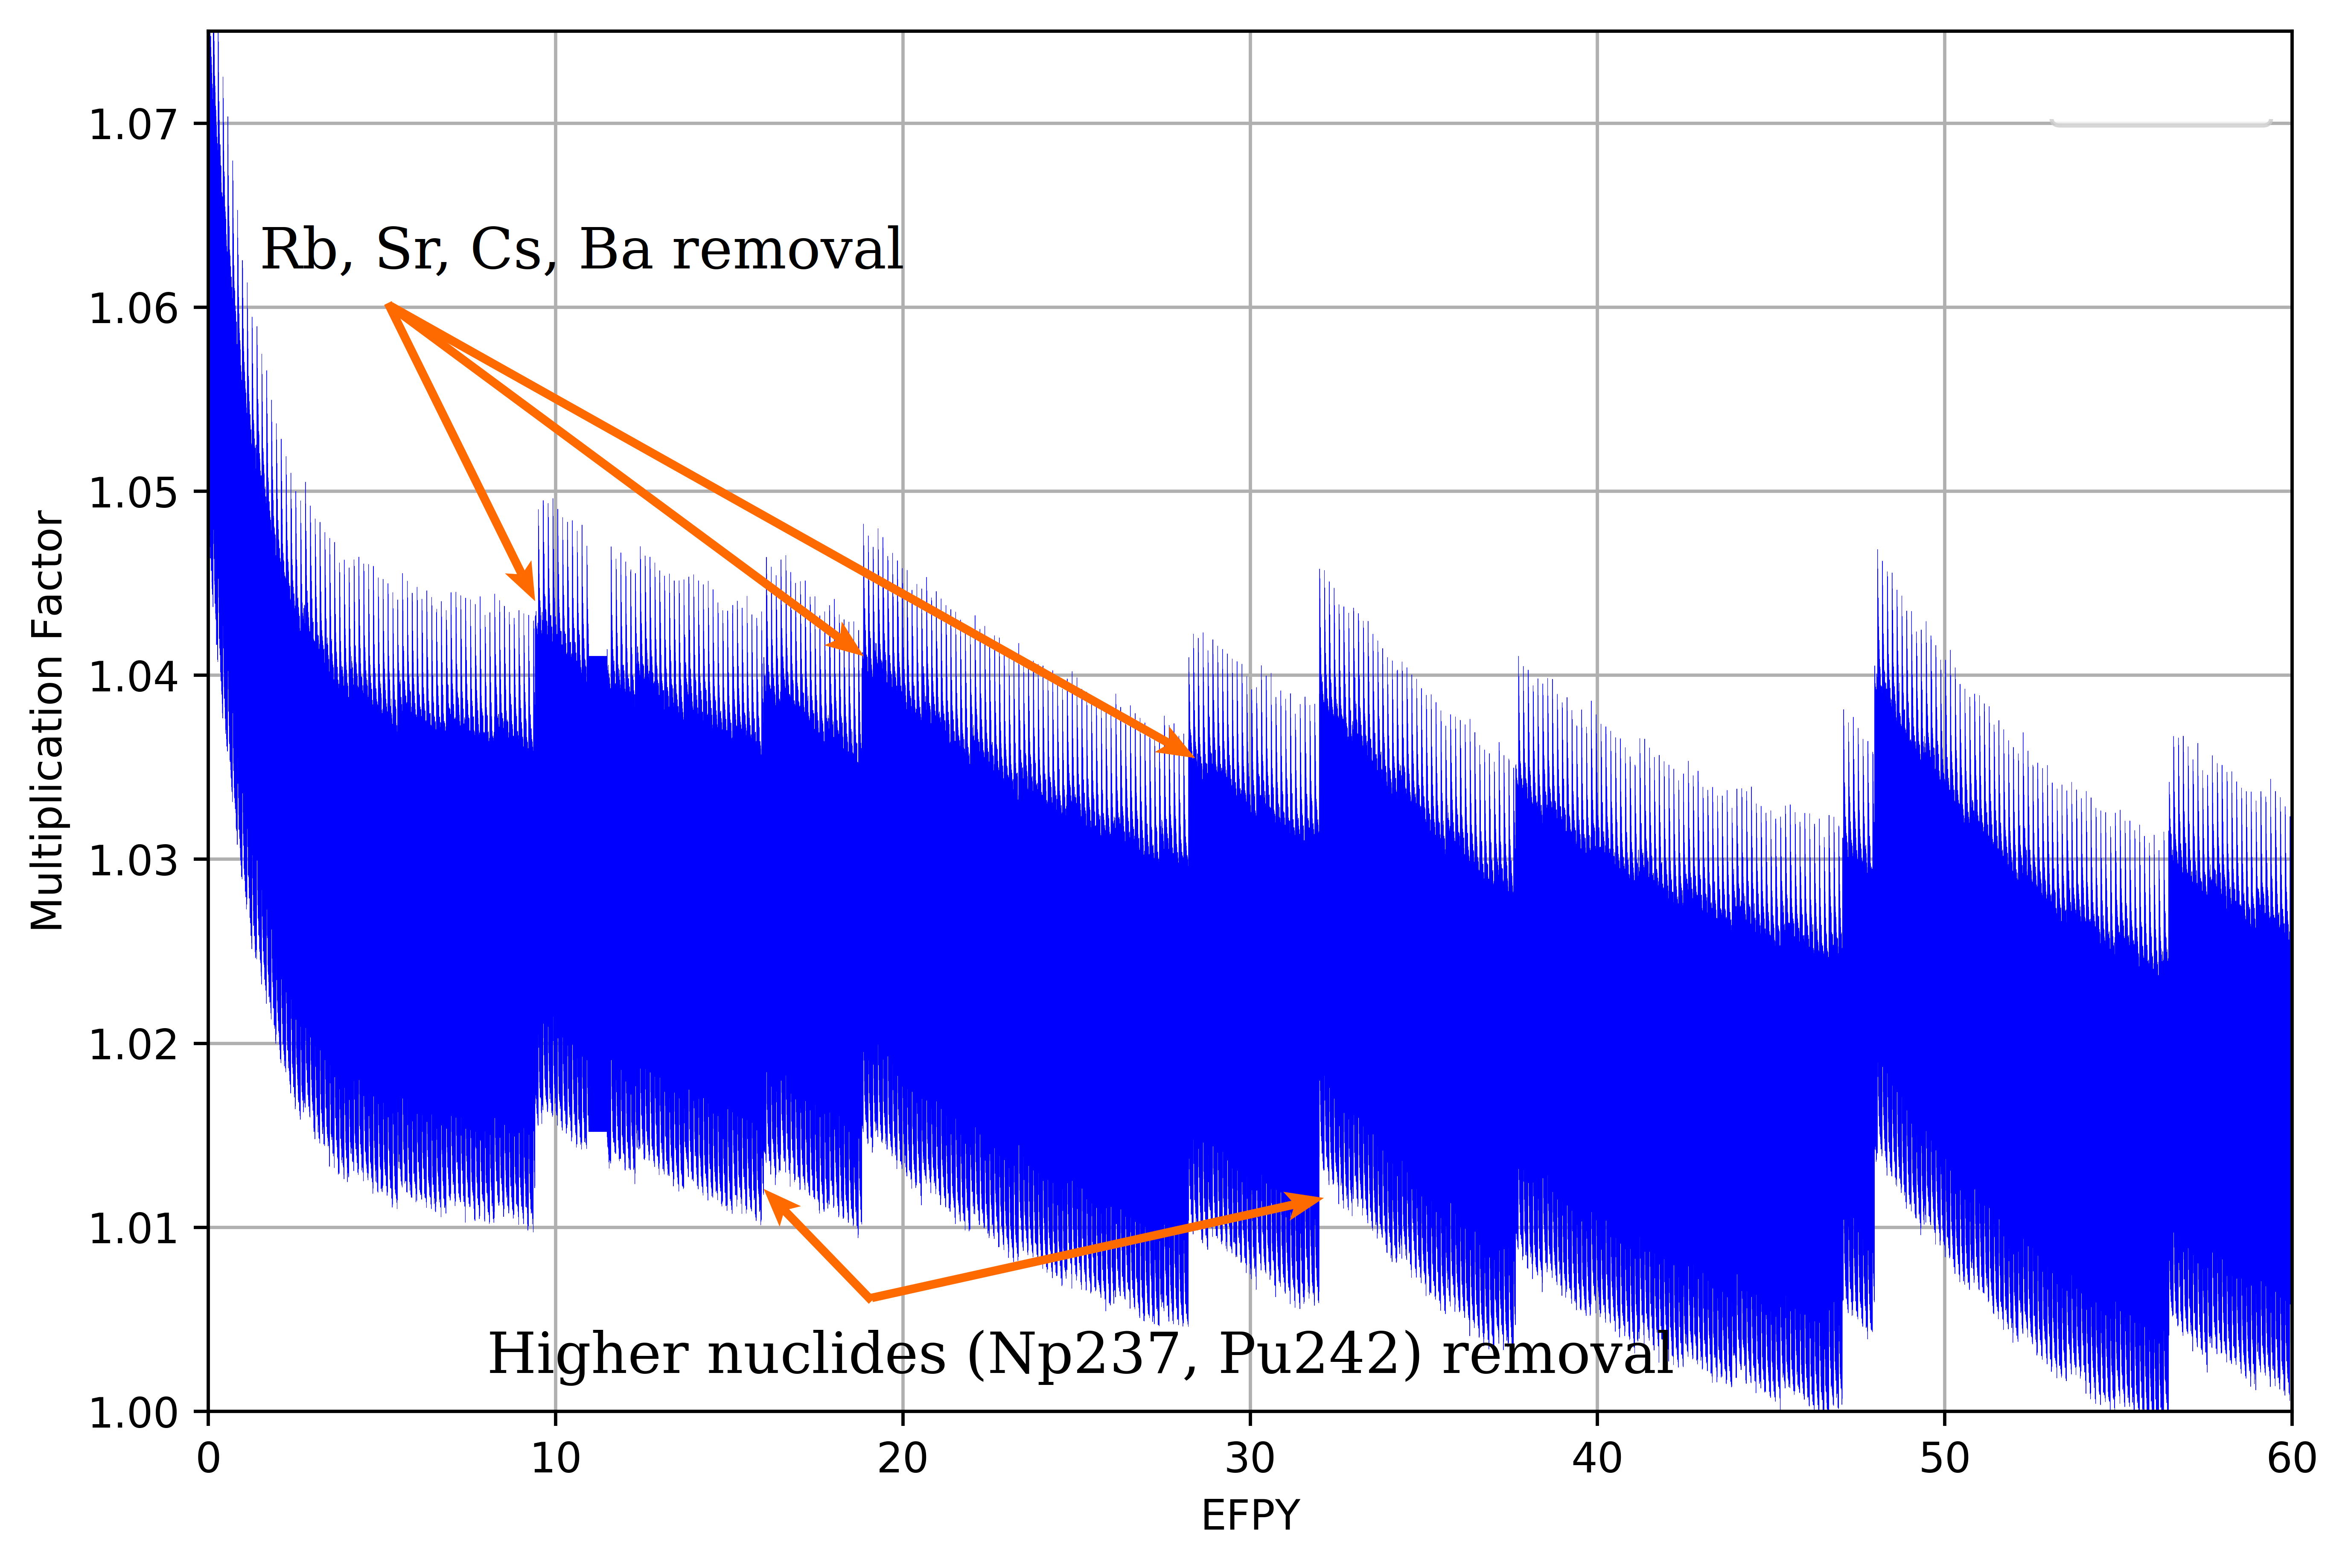
\includegraphics[width=\textwidth]{ch3/keff.png}
	\caption{Effective multiplication factor dynamics for full-core \gls{MSBR} 
		model over a 60-year reactor operation lifetime (reproduced 
		from Rykhlevskii \emph{et al.} \cite{rykhlevskii_modeling_2019}).}
	\label{fig:keff}
\end{figure}
\begin{figure}[ht!] 
	\centering
	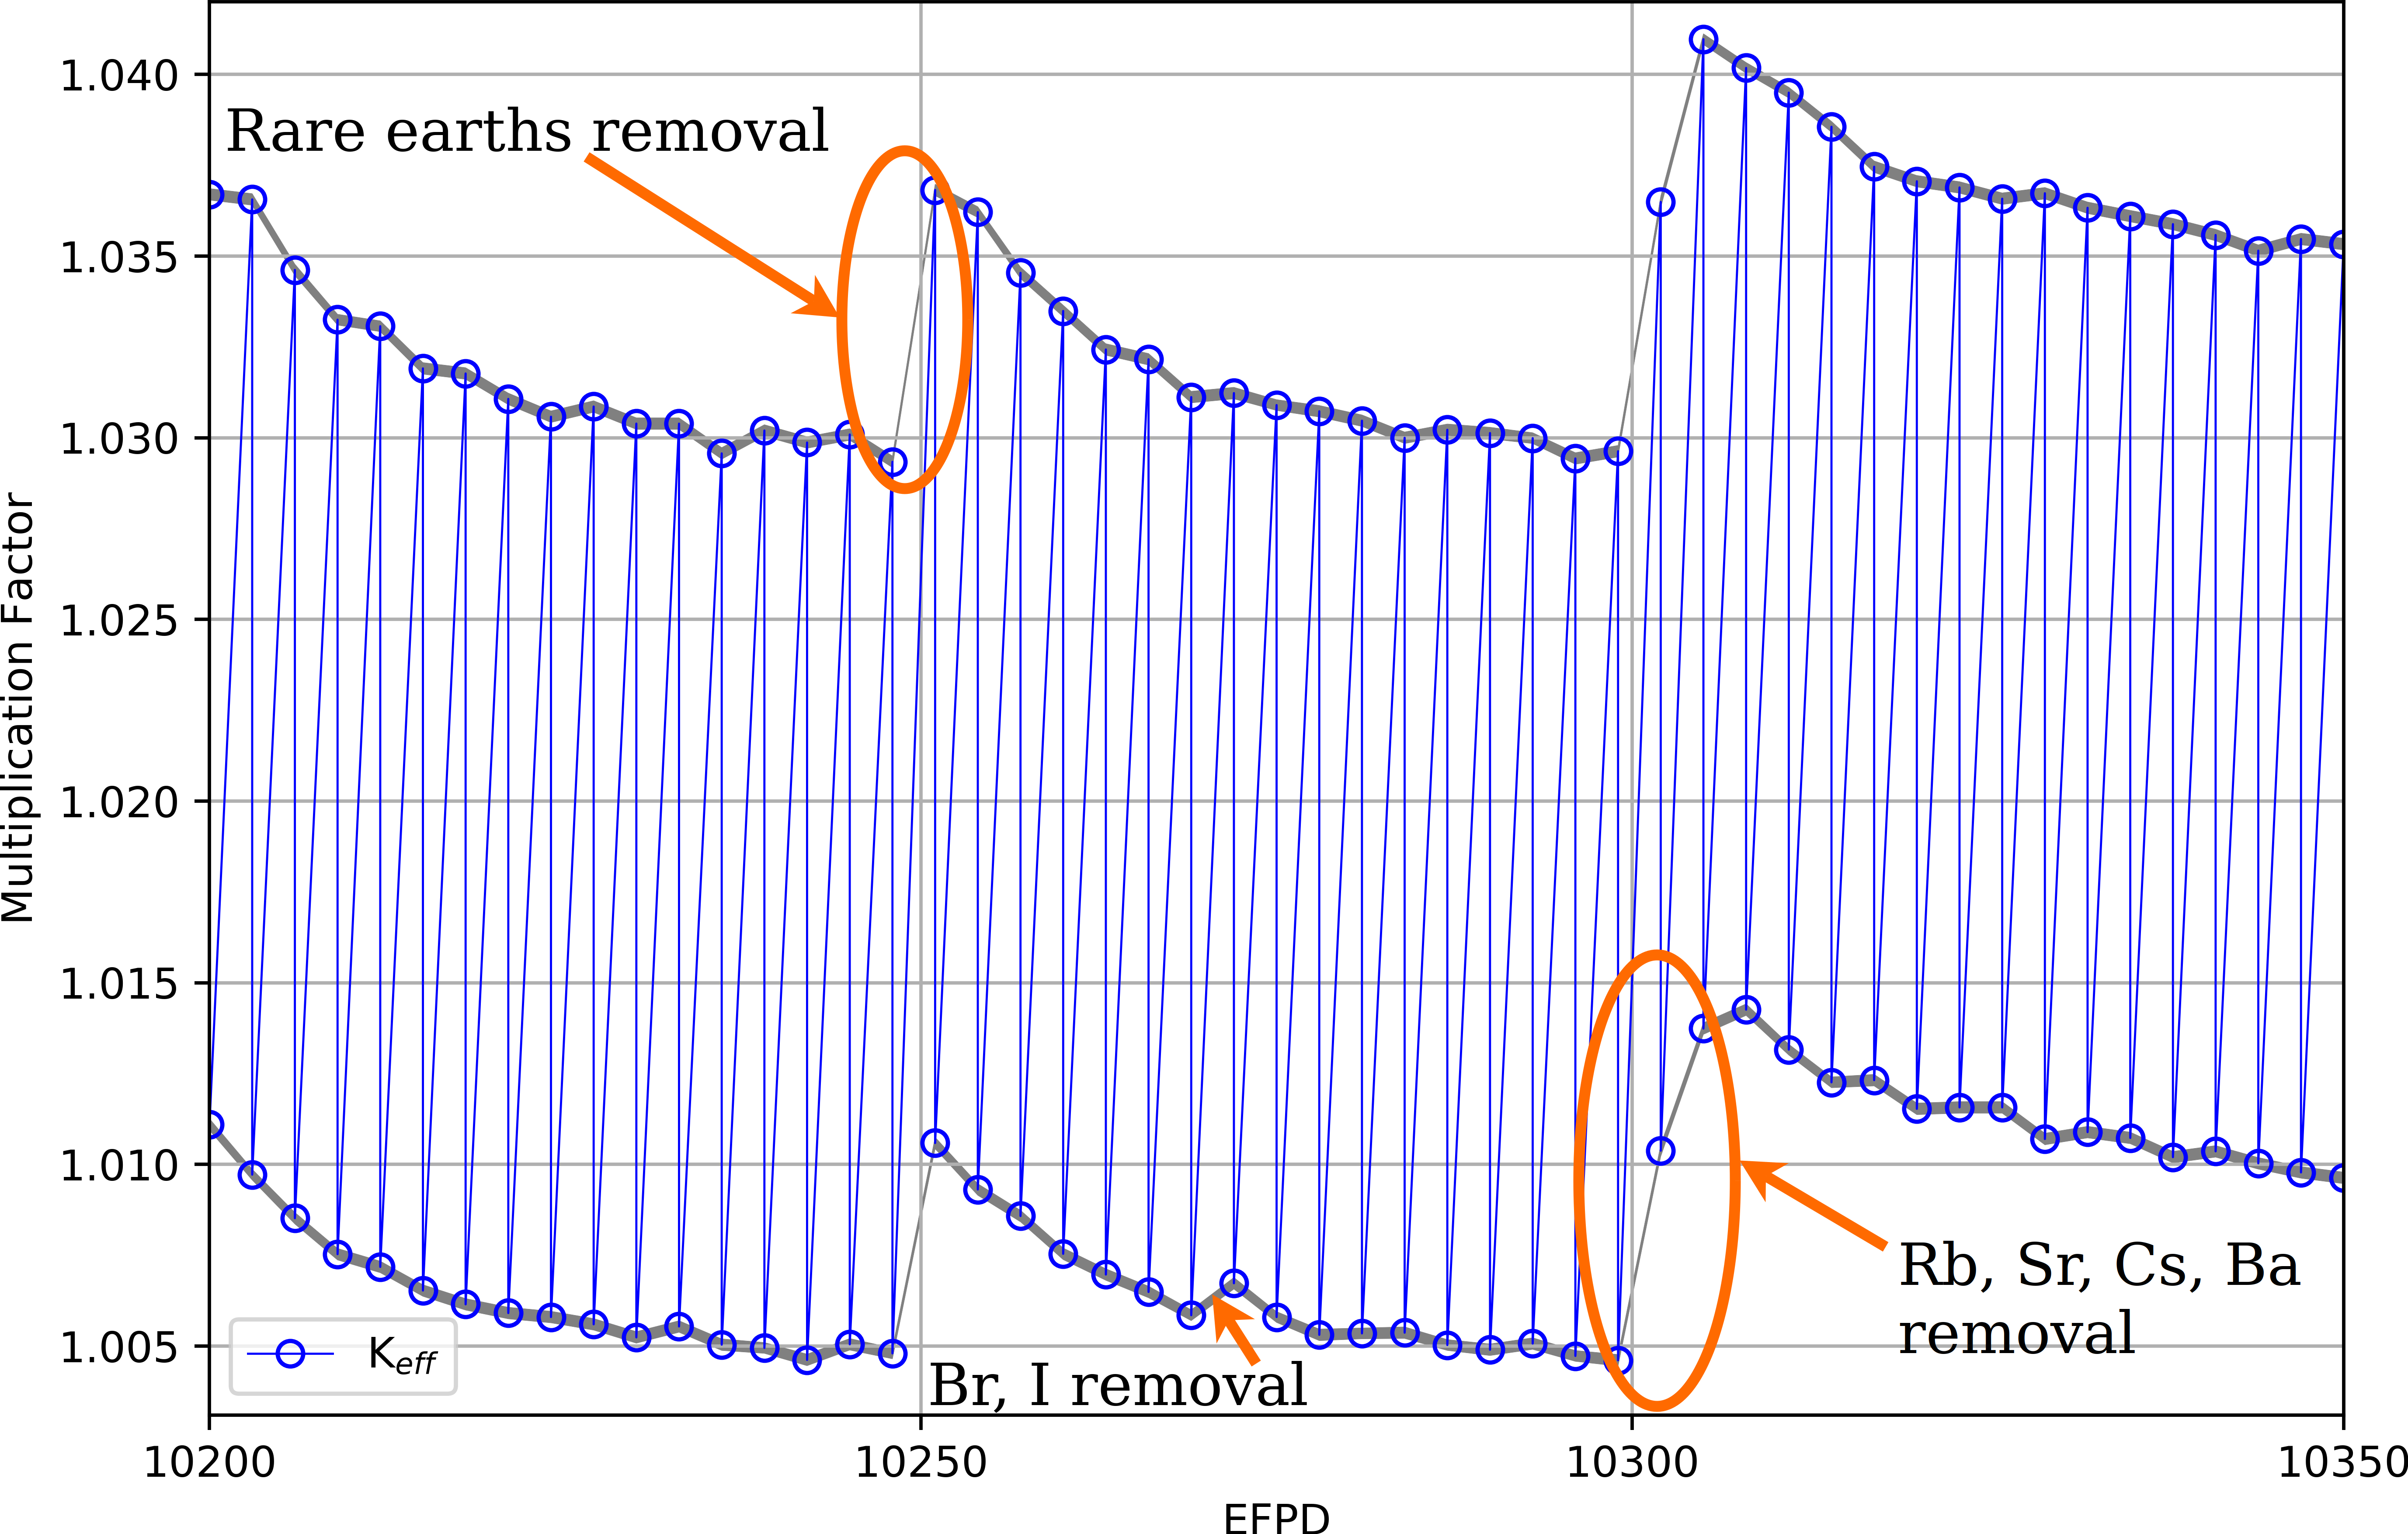
\includegraphics[width=\textwidth]{ch3/keff_zoomed.png}
	\caption{Zoomed effective multiplication factor for a 150-EFPD time 
	interval (reproduced from Rykhlevskii \emph{et al.}  
	\cite{rykhlevskii_modeling_2019}).}
	\label{fig:keff_zoomed}
\end{figure}

First, Serpent calculates the effective multiplication factor for the  
beginning of the cycle. 
Next, it computes the new fuel salt composition at the end of a 3-day 
depletion. The corresponding effective multiplication factor is much smaller 
than the previous one. Finally, Serpent calculates $k_{eff}$ for the depleted 
composition after applying feeds and removals. The $k_{eff}$ increases 
accordingly since major reactor poisons (e.g., Xe, Kr) are removed, while 
fresh fissile material ($^{233}$U) from the protactinium decay tank is added.  

Additionally, the presence of rubidium, strontium, cesium, and barium in the 
core are disadvantageous to reactor physics. Overall, the effective 
multiplication factor gradually decreases from 1.075 to $\approx$1.02 at 
equilibrium after approximately 6 years of irradiation. 

%In fact, SaltProc v0.1 fully removes all of these elements every 3435 days 
%(not a small mass fraction every 3 days) which causes the multiplication 
%factor to jump by approximately $450$ $pcm$, and limits using the batch 
%approach for online reprocessing simulations. In SaltProc v1.0 this drawback 
%has been eliminated by removing fraction of element at each depletion step 
%with 
%longer residence times (seminoble metals, volatile fluorides, Rb, Sr, Cs, Ba, 
%Eu). Results obtain with this approach will be presented for the \gls{TAP} 
%\gls{MSR} in chapter 4.


\subsection{Fuel salt composition dynamics}\label{sec:ch3-msbr-fuel-comp}
The analysis of the fuel salt composition evolution provides more 
comprehensive information about the equilibrium state. 
Figure~\ref{fig:adens_eq} shows the number densities of major nuclides, which 
have a strong influence on the reactor core physics. The concentration of 
$^{233}$U, $^{232}$Th, $^{233}$Pa, and $^{232}$Pa in the fuel salt change 
insignificantly after approximately 2500 days of operation. In particular, the 
$^{233}$U number density fluctuates by less than 0.8\% between 16 and 20 years 
of operation. Hence, a quasi-equilibrium state was achieved after 16 years of 
reactor operation.

In contrast, a wide variety of nuclides, including fissile isotopes (e.g.,  
$^{235}$U) and non-fissile strong absorbers (e.g., $^{234}$U), kept 
accumulating in the core. Figure~\ref{fig:fissile_short} demonstrates the 
production of fissile isotopes in the core. At the end of the considered 
operational time, the core contained significant $^{235}$U ($\approx10^{-5}$ 
atoms/b-cm), $^{239}$Pu ($\approx5\times10^{-7}$ atoms/b-cm), and $^{241}$Pu 
($\approx 5\times10^{-7}$ atoms/b-cm). Meanwhile, the equilibrium number 
density of the target fissile isotope $^{233}$U was approximately 
7.97$\times10^{-5}$ atoms/b-cm. Small dips in neptunium and plutonium number 
density every 16 years are caused by removing $^{237}$Np and $^{242}$Pu 
(included in Processing group ``Higher nuclides'', see 
Table~\ref{tab:reprocessing_list_msbr}) which decay into $^{235}$Np and 
$^{239}$Pu, respectively. Thus, the production of new fissile materials in the 
core, as well as $^{233}$U breeding, made it possible to compensate for the 
negative effects of strong absorber accumulation ($^{234}$U) and keep the 
reactor critical.
\begin{figure}[ht!] % replace 't' with 'b' to 
	\centering
	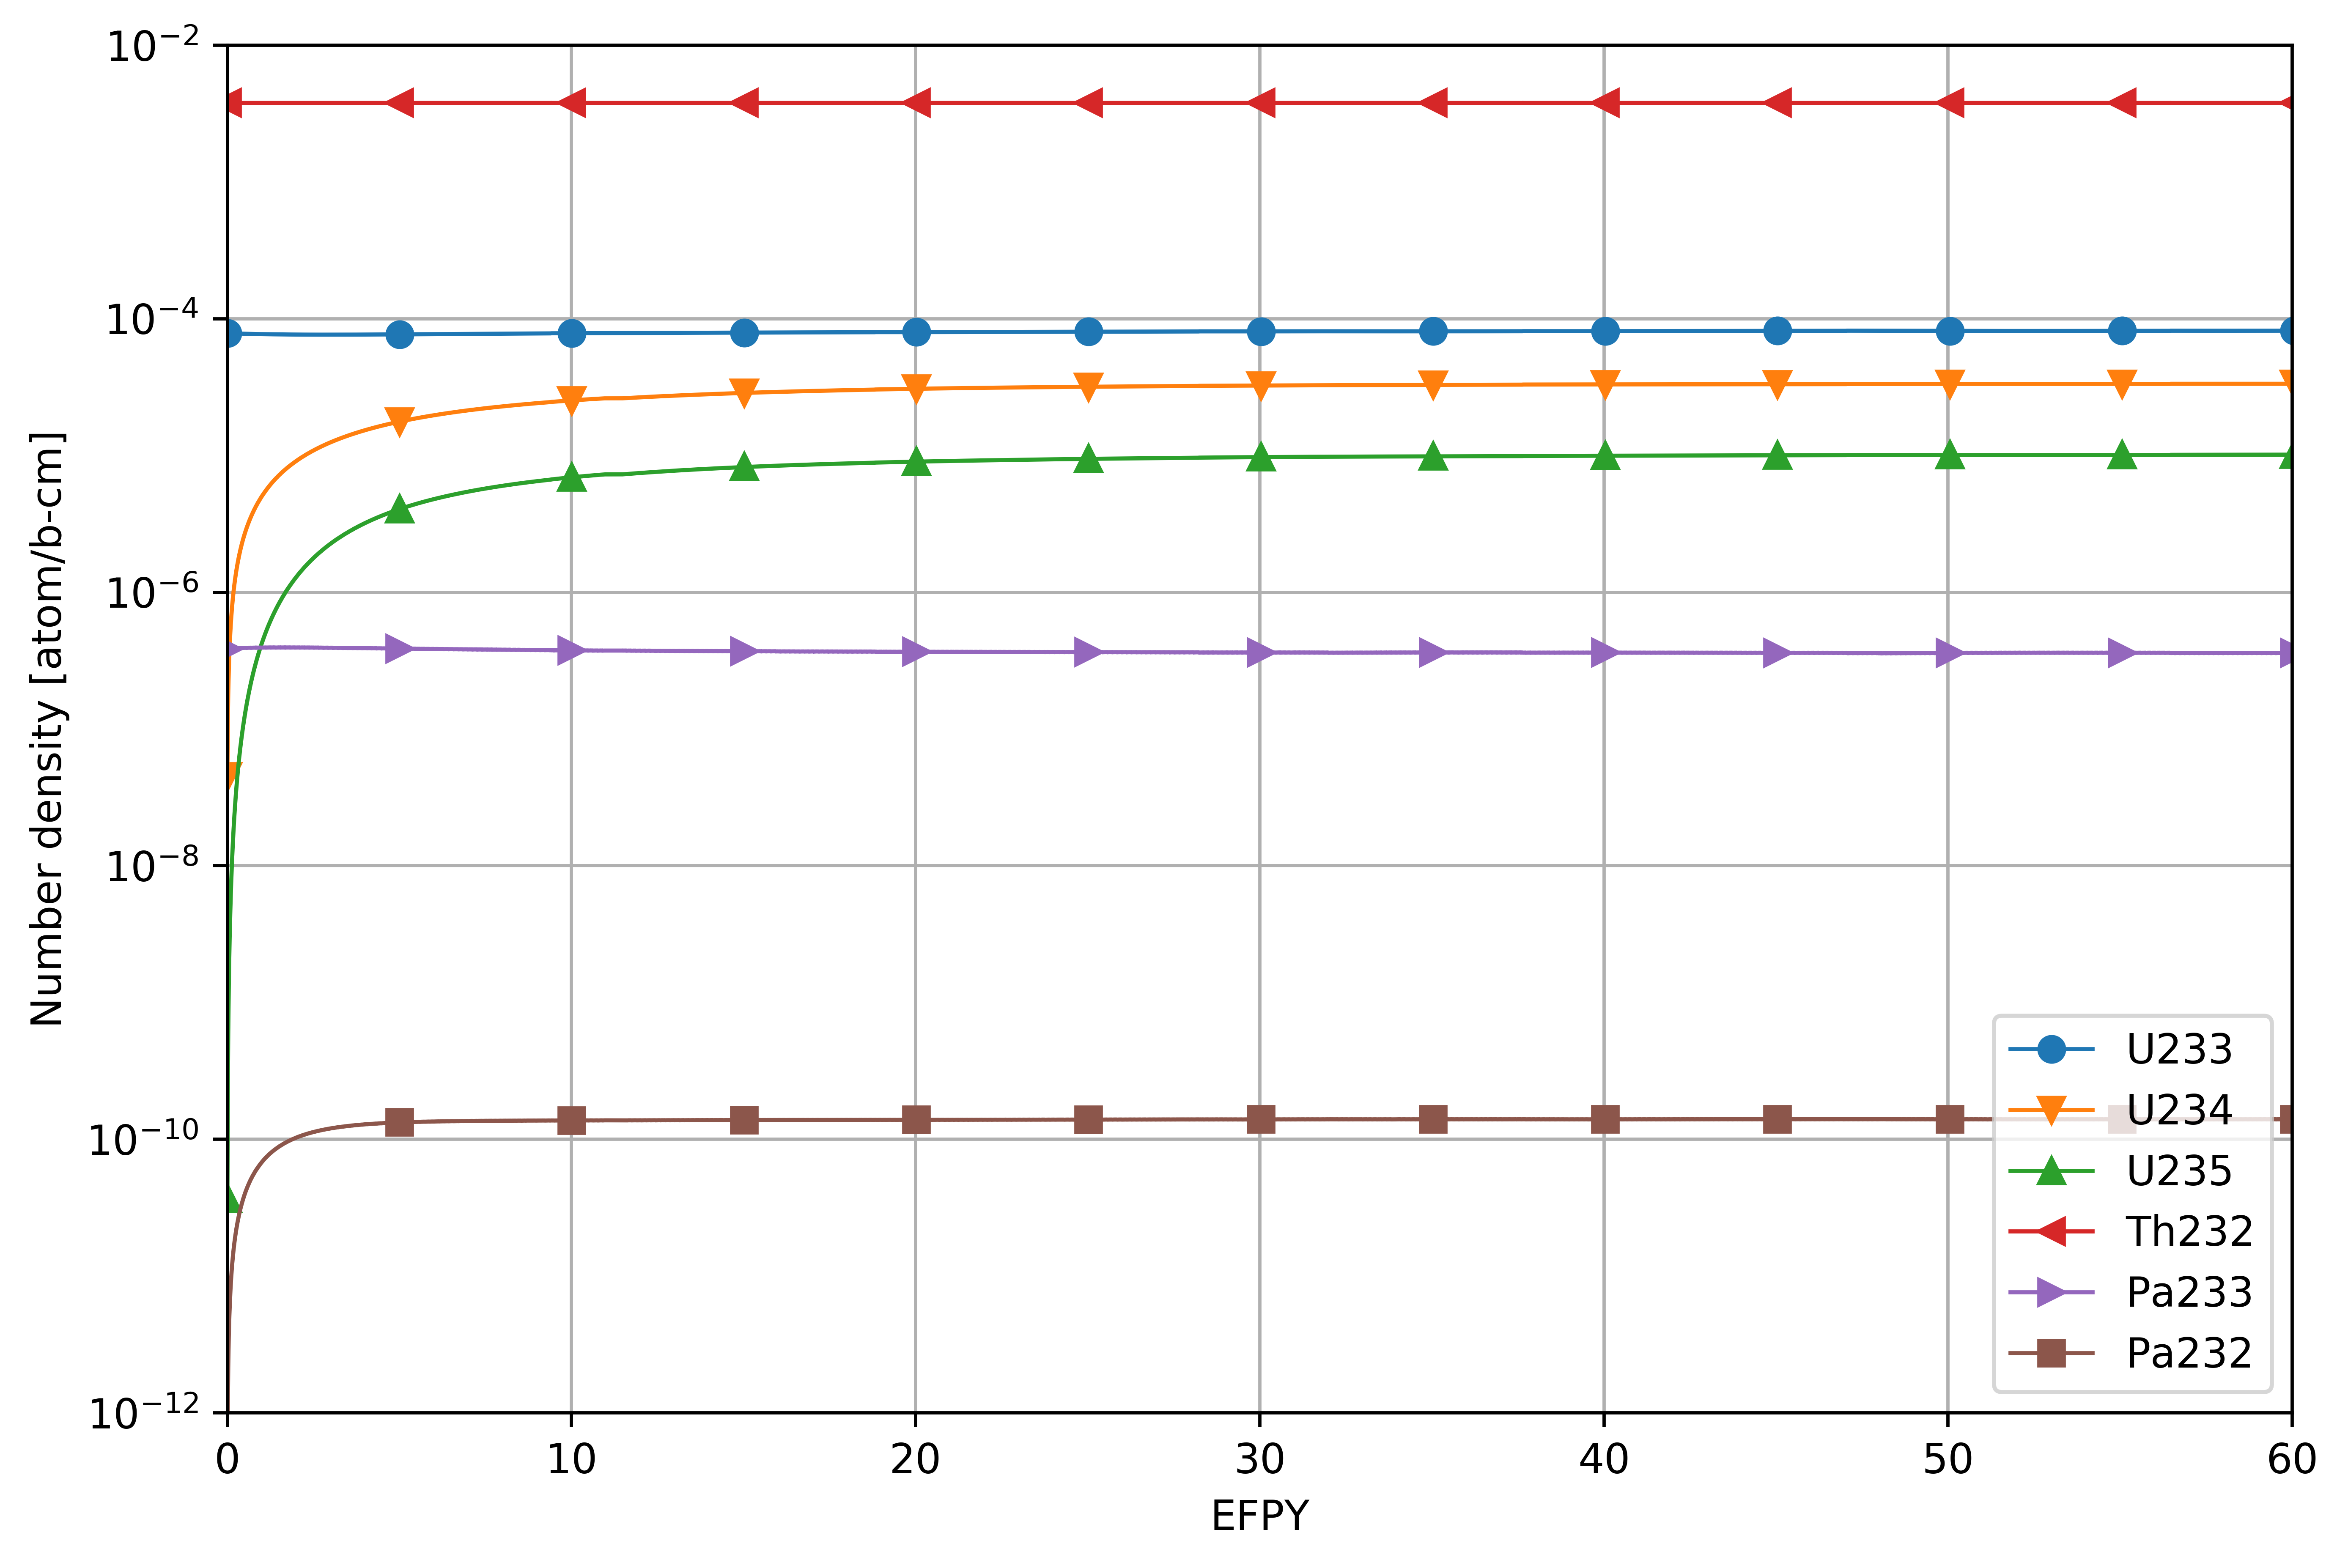
\includegraphics[width=\textwidth]{ch3/major_isotopes_adens.png}
	\caption{The number density of major nuclides during 60 years of reactor 
		operation (reproduced from Rykhlevskii \emph{et al.}  
		\cite{rykhlevskii_modeling_2019}).}
	\label{fig:adens_eq}
\end{figure}
\begin{figure}[t] % replace 't' with 'b' to 
	\centering
	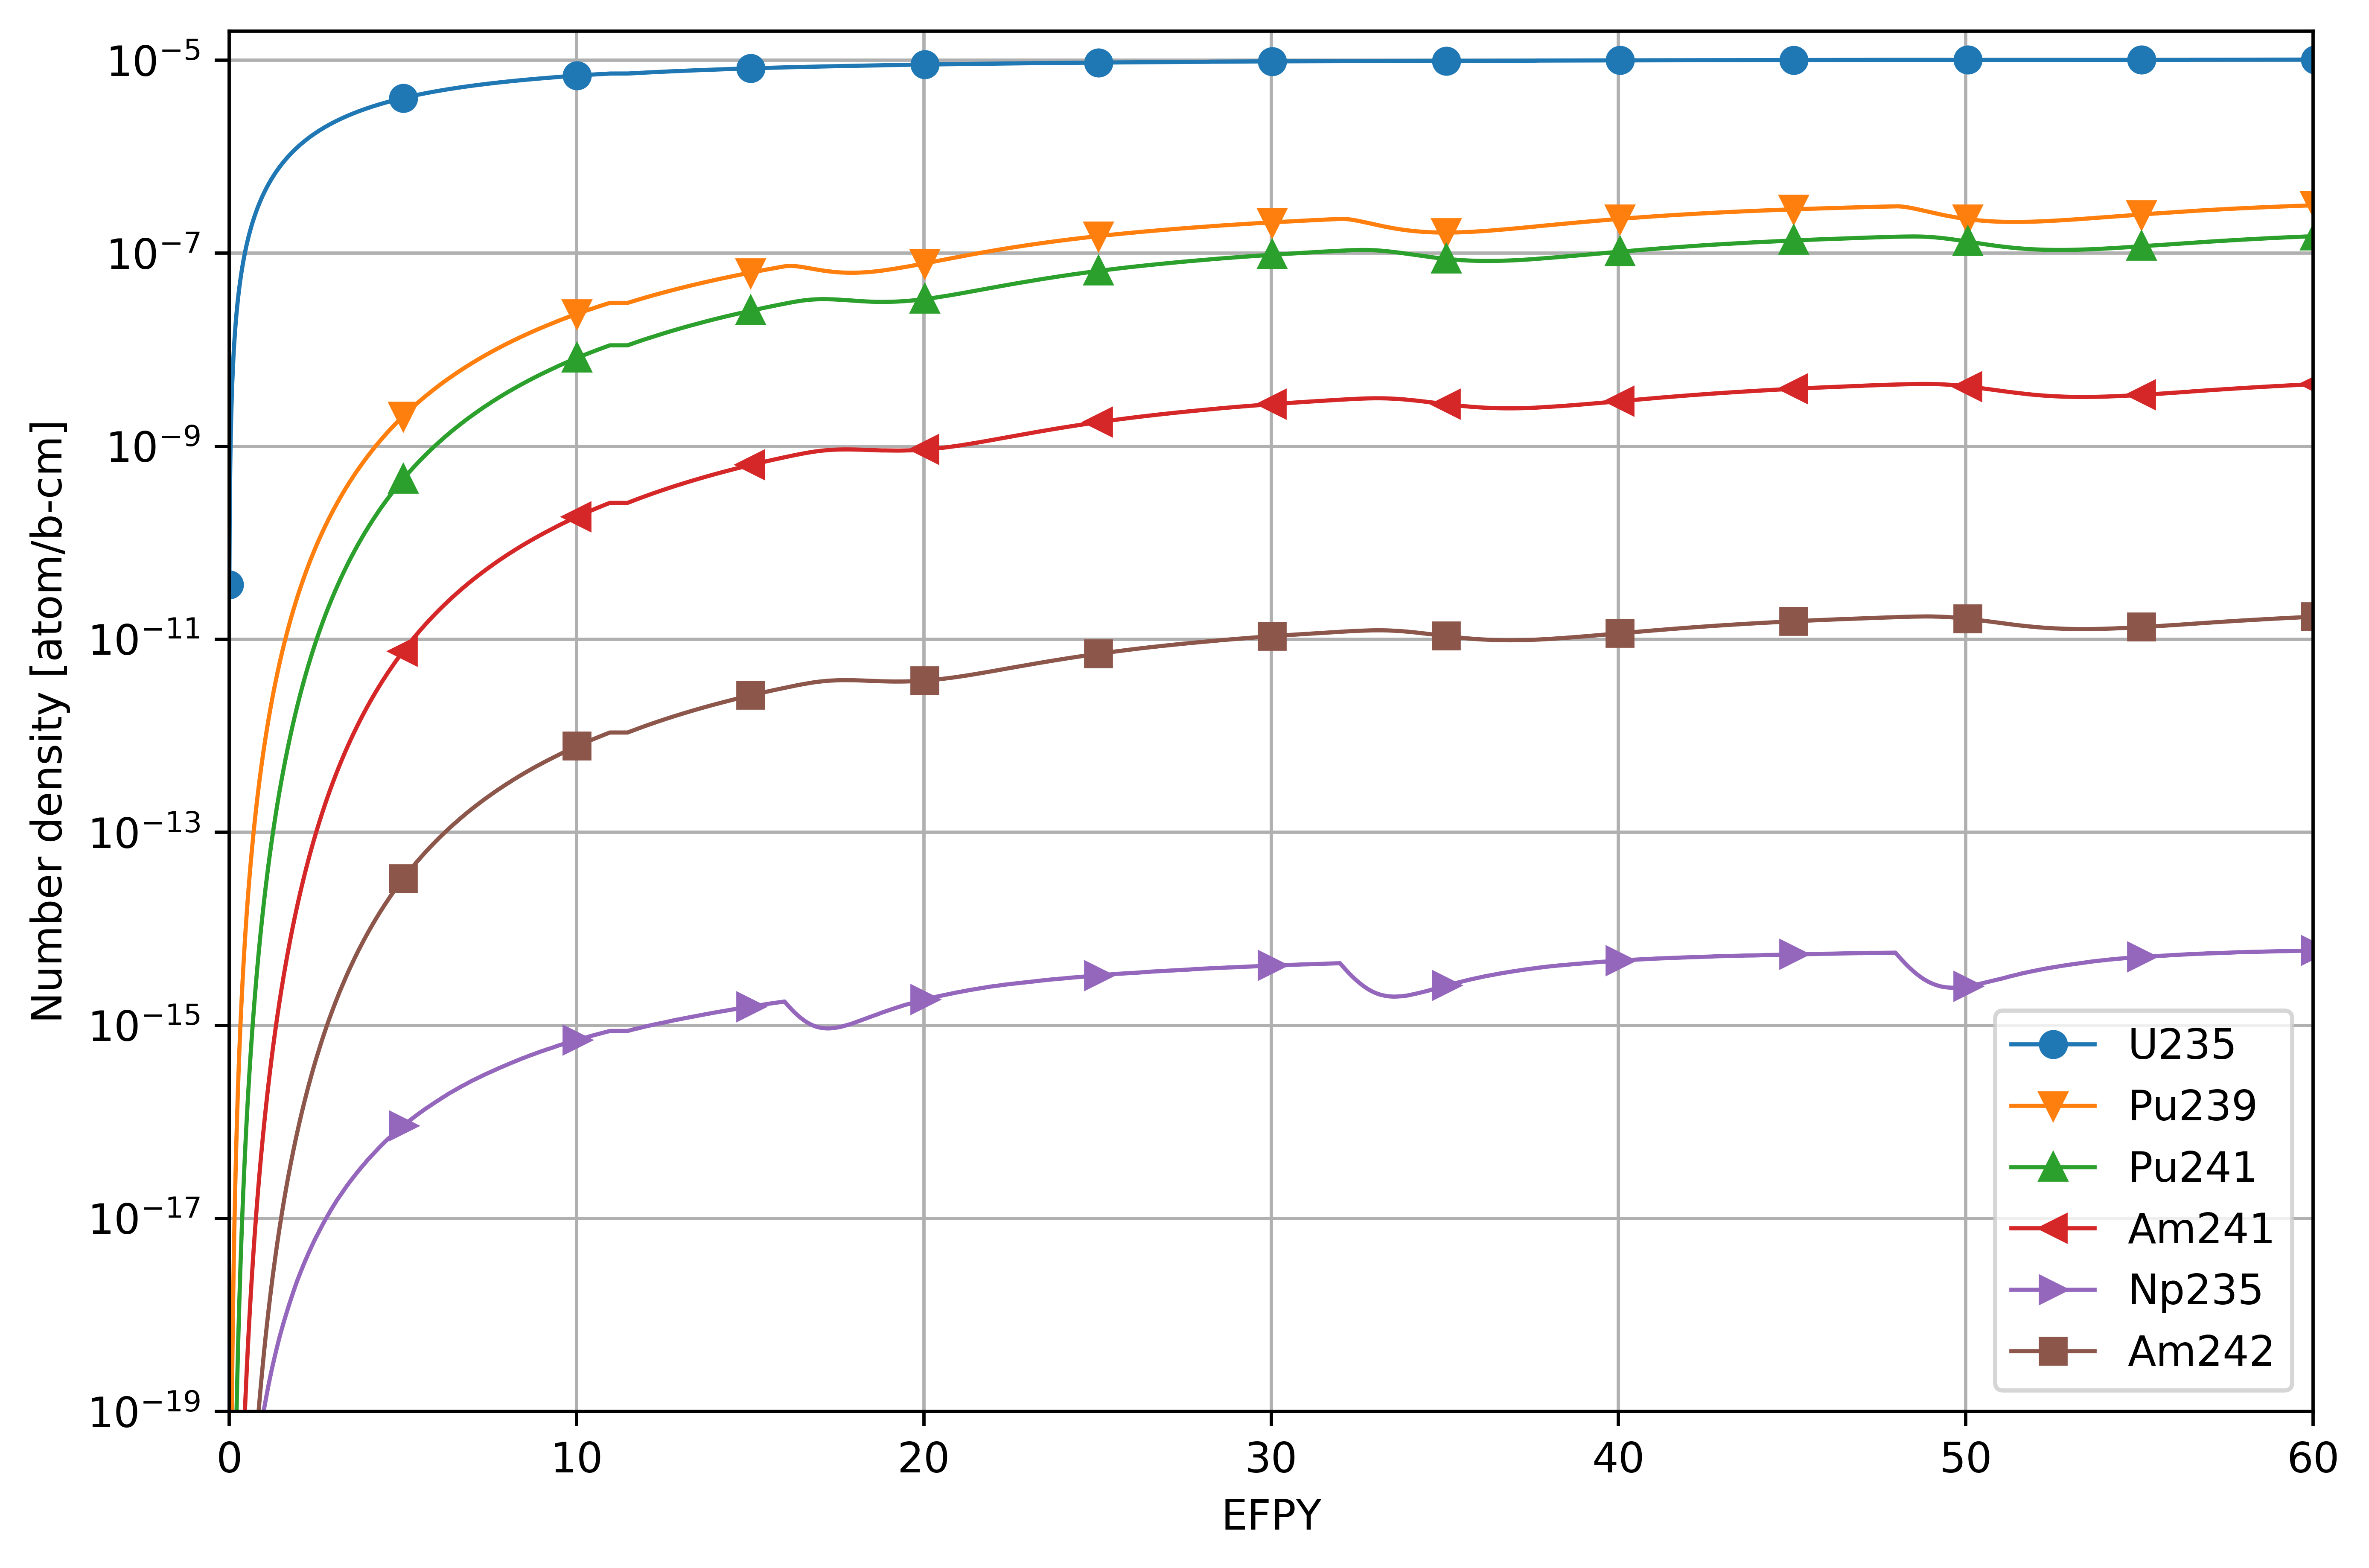
\includegraphics[width=\textwidth]{ch3/fissile_short.png}
	\vspace{-6mm}
	\caption{The number density of \emph{fissile in epithermal spectrum} 
	nuclides during 60 years of the reactor operation (reproduced from 
		Rykhlevskii \emph{et al.} \cite{rykhlevskii_modeling_2019}).}
	\label{fig:fissile_short}
\end{figure}
\FloatBarrier

\subsection{Neutron spectrum}
Figure~\ref{fig:spectrum} shows the normalized neutron flux spectrum for the 
full-core \gls{MSBR} model in the energy range from $10^{-8}$ to $10$ MeV. The 
neutron energy spectrum at equilibrium is harder than at startup due to 
plutonium and other strong absorbers accumulating in the core during reactor 
operation.  

Figure~\ref{fig:spectrum_zones} shows that zone I produced more thermal  
neutrons than zone II, corresponding to a majority of fissions occurring in 
the central part of the core. In the undermoderated zone II, the neutron 
energy spectrum is harder, which leads to more intensive neutron capture by 
$^{232}$Th and helps achieve a relatively high breeding ratio. Moreover, the 
(n,$\gamma$) resonance energy range in $^{232}$Th is from 10$^{-4}$ to 
10$^{-2}$ MeV. Thus, the moderator-to-fuel ratio for zone II was chosen 
to shift the neutron energy spectrum in this range. Furthermore, in the 
central core region (zone I), the neutron energy spectrum shifts to a harder 
spectrum over 20 years of reactor operation; meanwhile, in the outer core 
region (zone II), a similar spectral shift takes place at a reduced scale. 
These results are in good agreement with the original ORNL report 
\cite{robertson_conceptual_1971} and the most recent whole-core steady-state 
study \cite{park_whole_2015}.
\begin{figure}[htp!] % replace 't' with 'b'         to force it to 
	\centering
	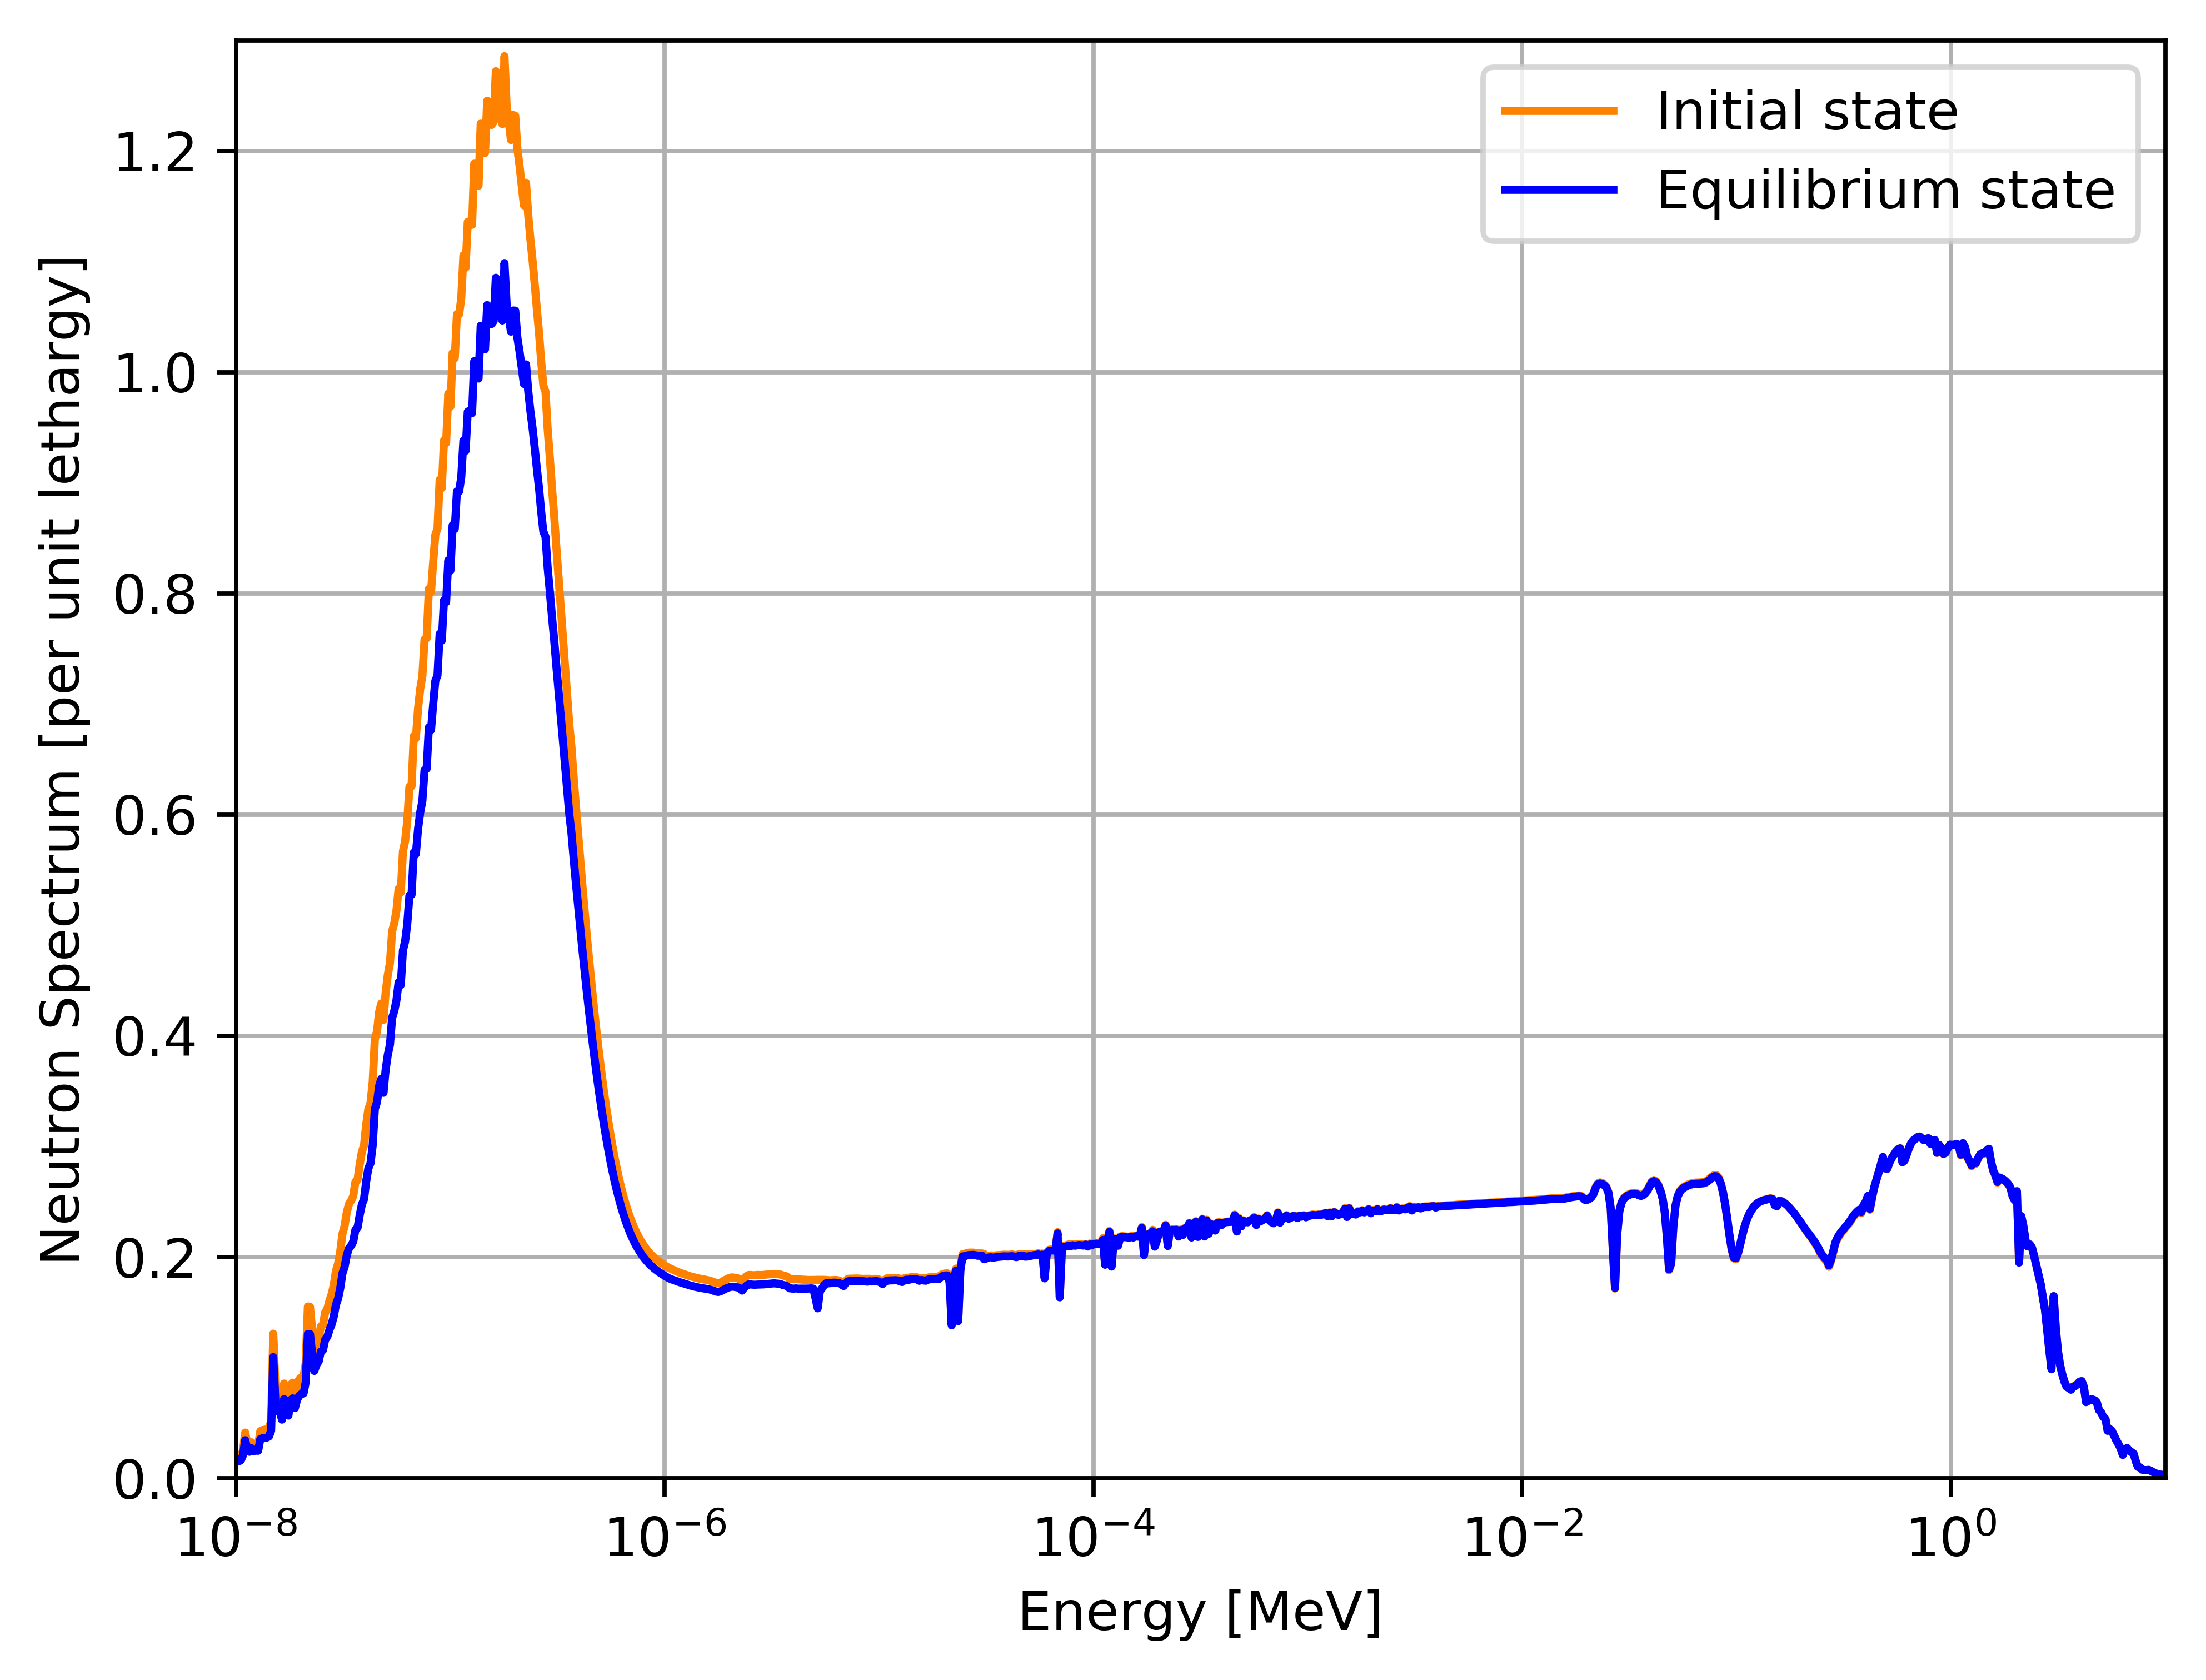
\includegraphics[width=0.85\textwidth]{ch3/spectrum.png}
	\caption{The neutron flux energy spectrum for initial and equilibrium  
	state normalized by unit lethargy (reproduced from Rykhlevskii 
	\emph{et al.} \cite{rykhlevskii_modeling_2019}).}
	\label{fig:spectrum}
\end{figure}
\begin{figure}[htp!] % replace 't' with 'b' to force it to 
	\centering
	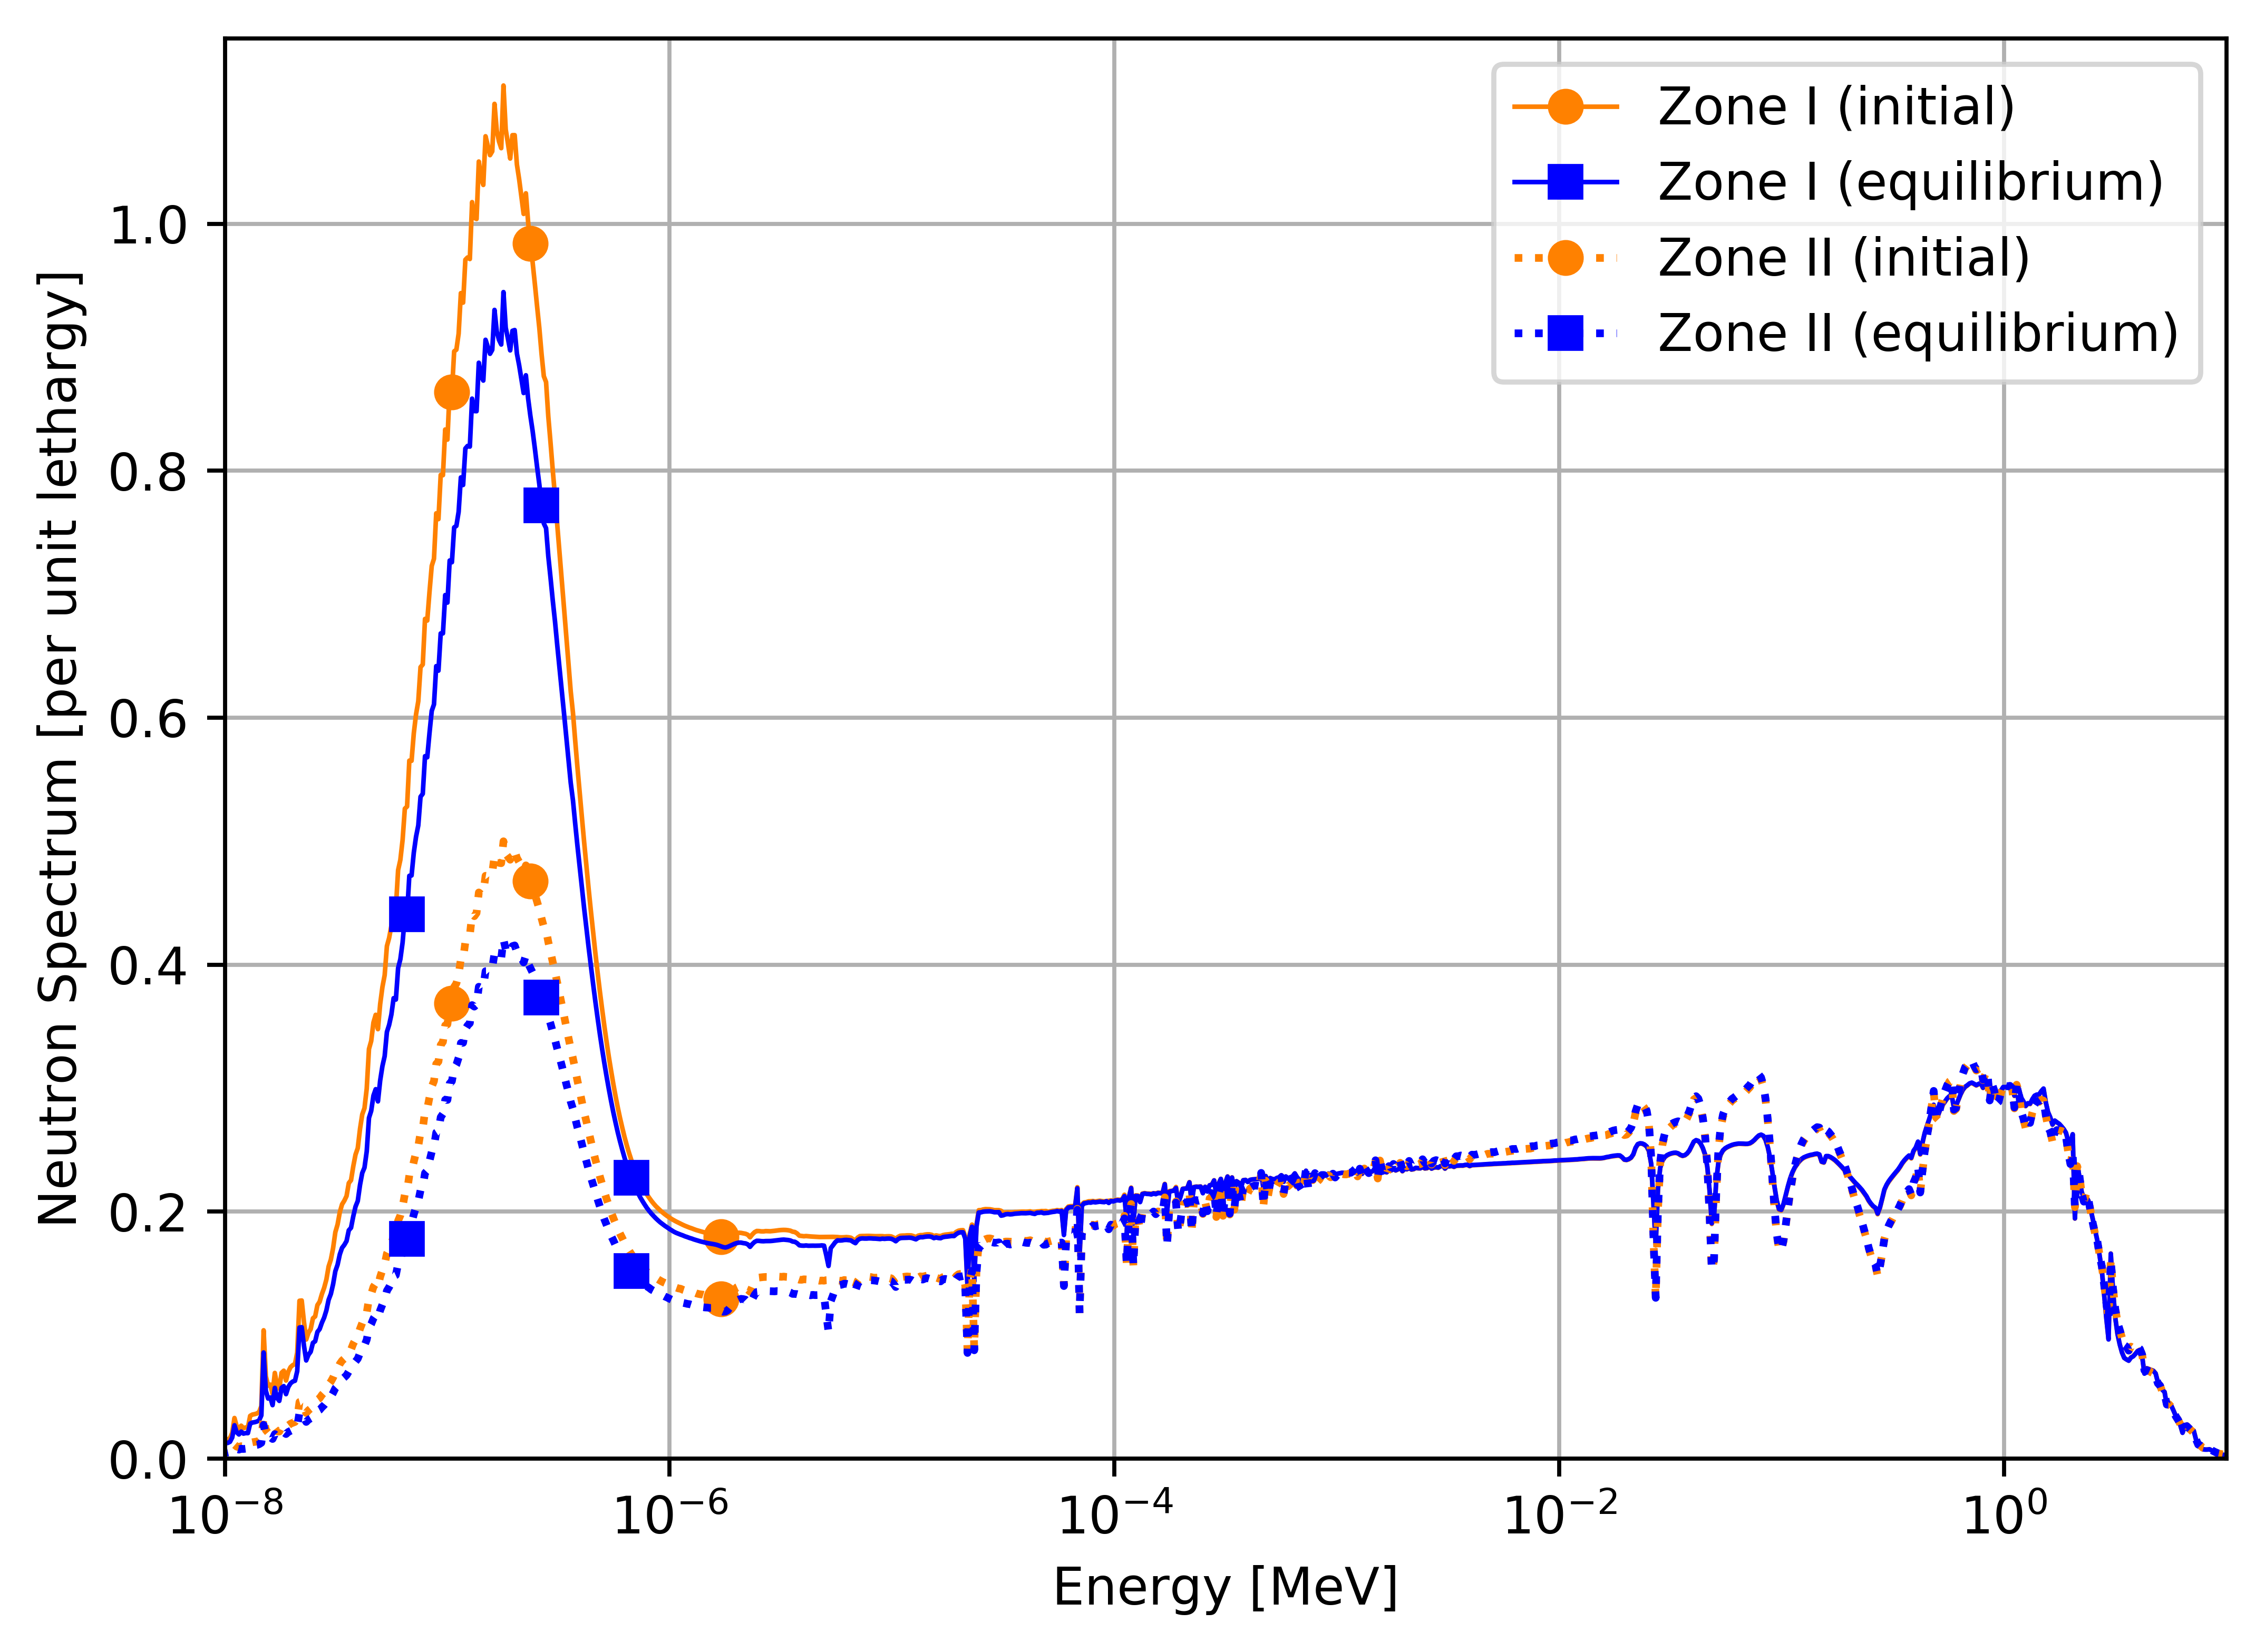
\includegraphics[width=0.85\textwidth]{ch3/spectrum_zones.png} 
	\caption{The neutron flux energy spectrum for initial and equilibrium  
		state normalized by unit lethargy (reproduced from 
		Rykhlevskii \emph{et al.} \cite{rykhlevskii_modeling_2019}).}
	\label{fig:spectrum_zones}
\end{figure}

It is important to obtain the epithermal and thermal spectra to produce 
$^{233}$U from $^{232}$Th because the radiative capture cross section of 
thorium decreases monotonically from $10^{-10}$ MeV to $10^{-5}$ MeV. 
Hardening the spectrum tends to significantly increase resonance absorption in 
thorium and decrease absorptions in fissile and construction materials. 

\subsection{Neutron flux}
Figure~\ref{fig:radial_flux} shows the radial distribution of fast and thermal 
neutron flux for initial and equilibrium compositions. The neutron fluxes have 
similar shapes for both compositions, but the equilibrium case has a harder 
spectrum. A significant spectral shift was observed in the central region of 
the core (zone I). In the outer region (zone II), annulus and graphite 
reflector, spectral shift is negligible. These neutron flux radial 
distributions agree with the fluxes in the original ORNL report 
\cite{robertson_conceptual_1971}. 
Overall, spectrum hardening during \gls{MSBR} operation should be carefully 
studied when designing the reactivity control system.
\begin{figure}[ht!] % replace 't' with 'b' to force it to \centering
	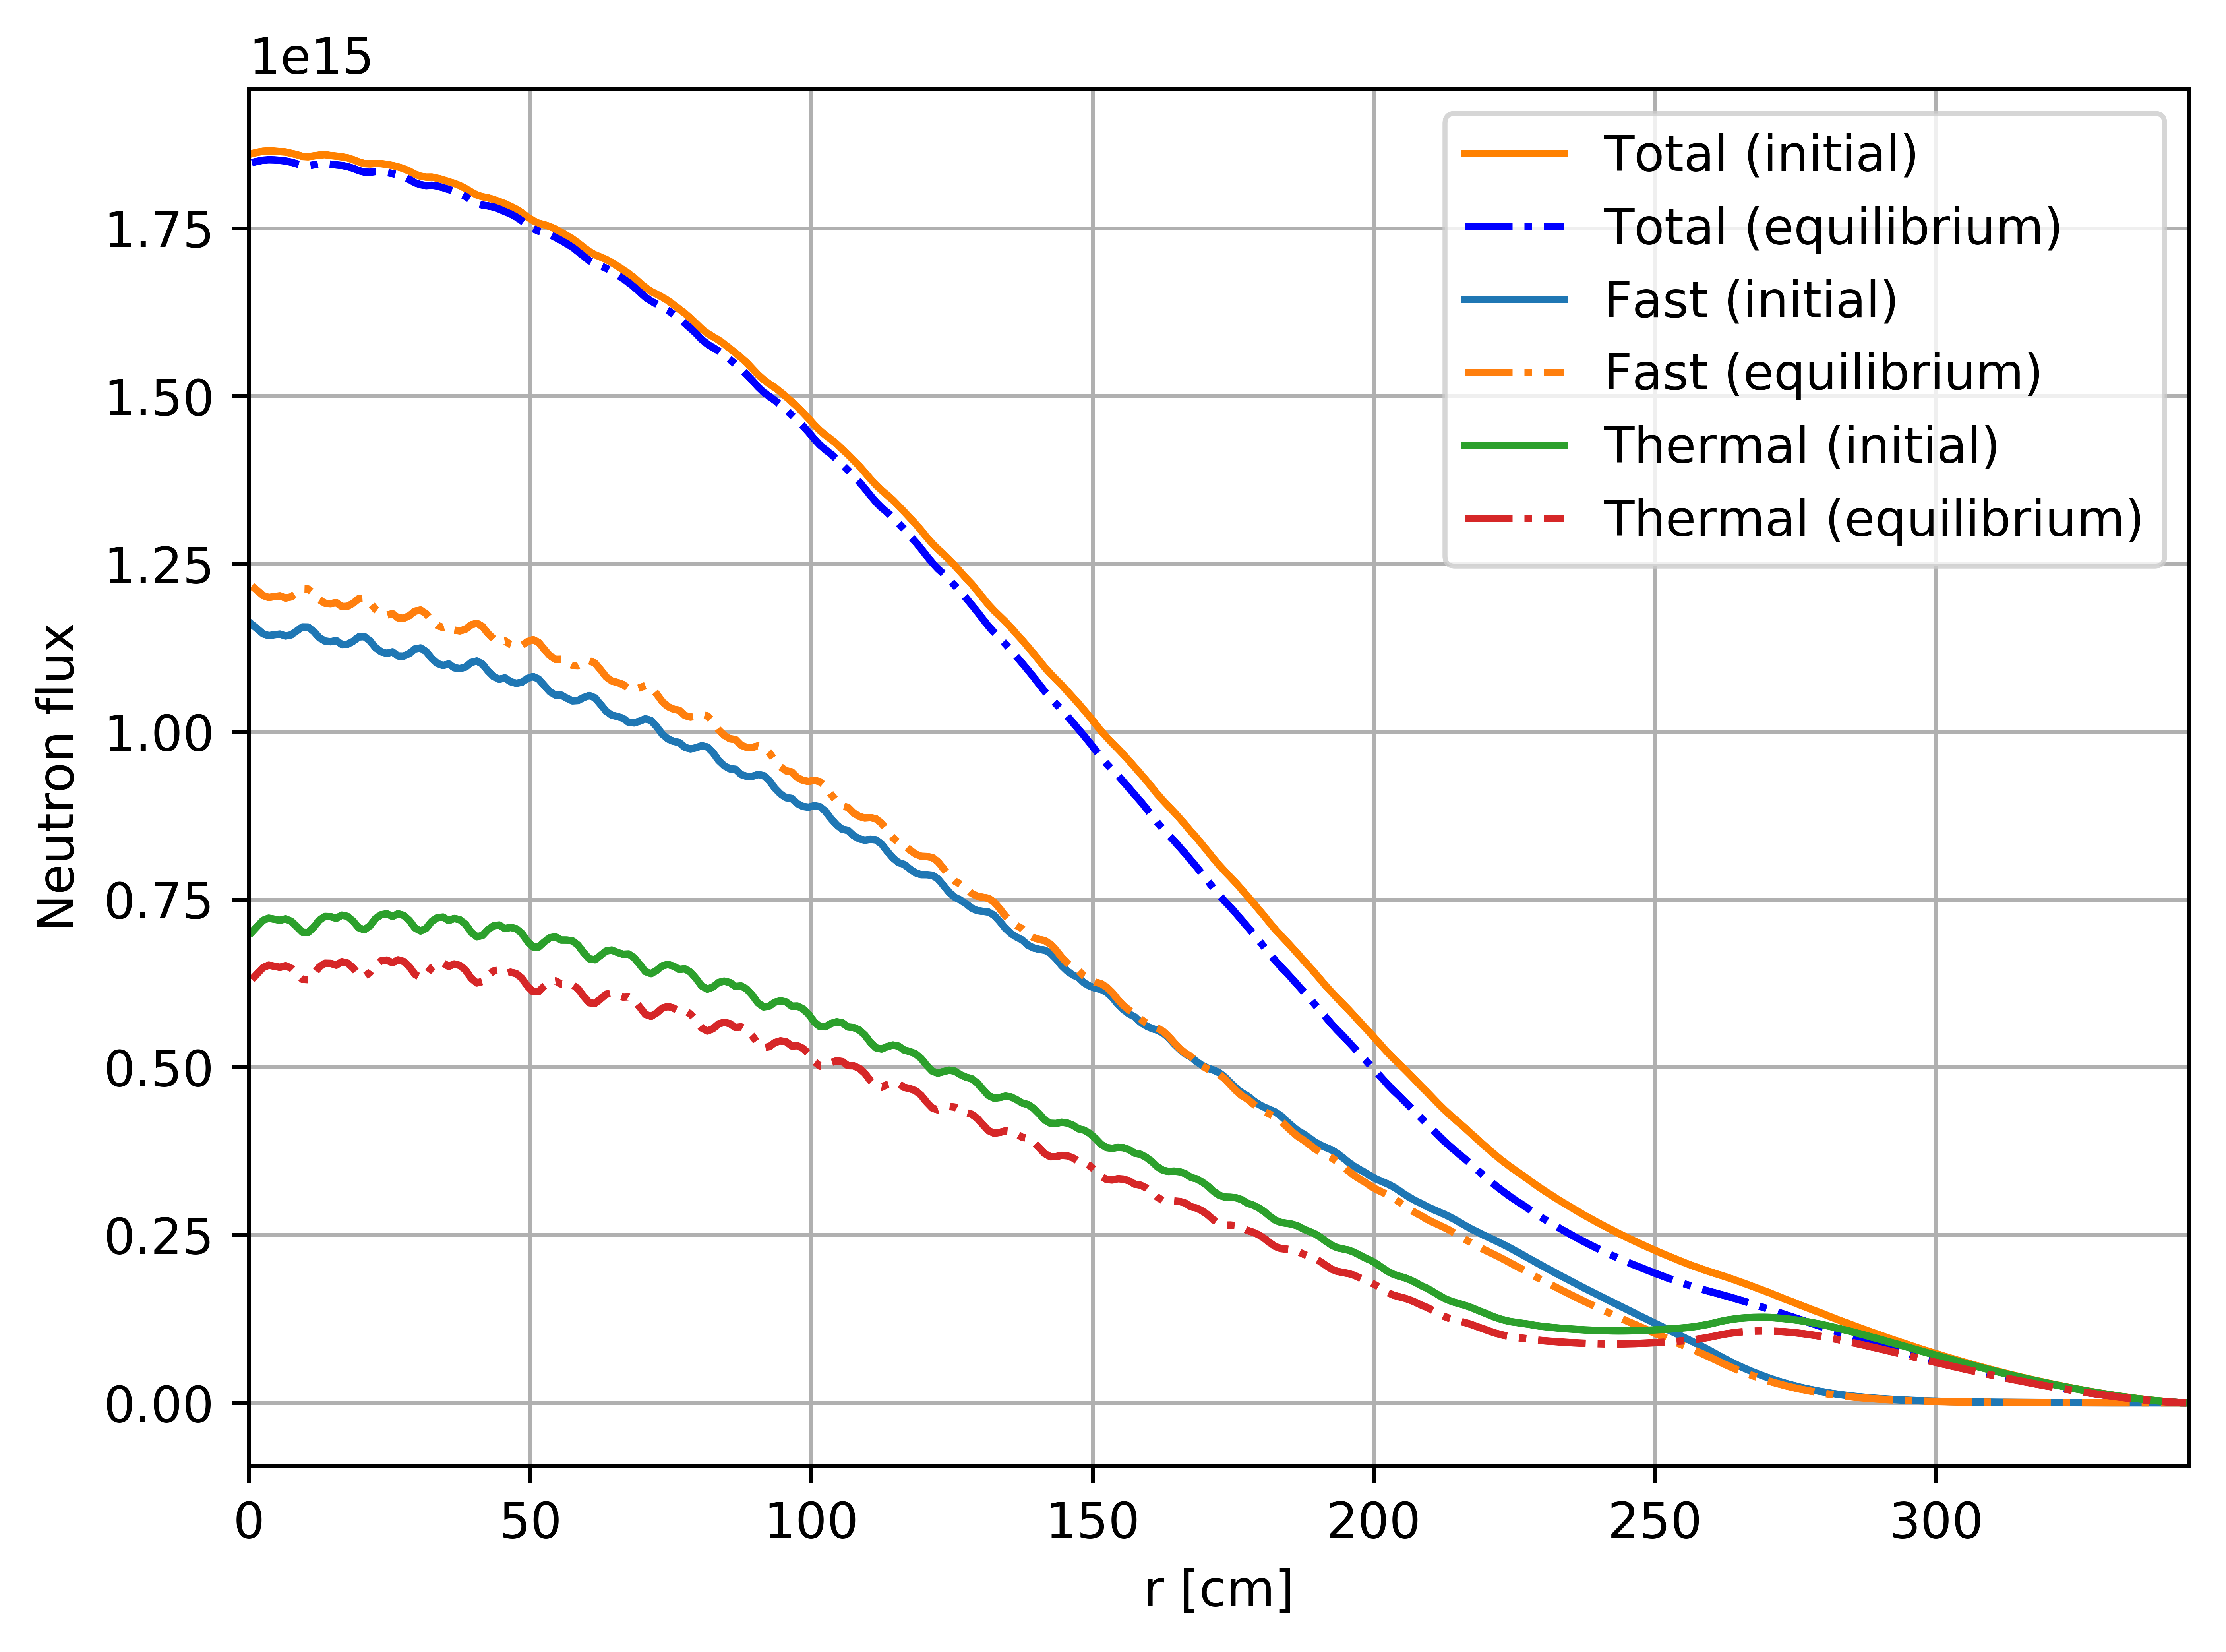
\includegraphics[width=\textwidth]{ch3/radial_flux.png}
	\caption{Radial neutron flux distribution for initial and equilibrium fuel 
	salt compositions (reproduced from Rykhlevskii \emph{et al.} 
	\cite{rykhlevskii_modeling_2019}).}
	\label{fig:radial_flux}
\end{figure}

\subsection{Power and breeding distribution}
Table~\ref{tab:powgen_fraction} shows the power fraction in each zone for 
initial and equilibrium fuel compositions. Figure~\ref{fig:pow_den} reflects 
the normalized power distribution of the \gls{MSBR} quarter core for 
equilibrium fuel salt composition. For both the initial and equilibrium 
compositions, fission primarily occurs in the center of the core, namely zone 
I. The spectral shift during reactor operation results in slightly different 
power fractions at startup and equilibrium, but most of the power is still 
generated in zone I at equilibrium (Table~\ref{tab:powgen_fraction}). 
%%%%%%%%%%%%%%%%%%%%%%%%%%%%%%%%%%%%%%%%
\begin{table}[ht!]
	\caption{Power generation fraction in each zone for initial and 
	equilibrium state (reproduced from Rykhlevskii \emph{et al.} 
	\cite{rykhlevskii_modeling_2019}).}
		\centering
	\begin{tabularx}{0.8\textwidth}{L R R} \hline
		Core region & Initial            & Equilibrium   \\   \hline
		Zone I      & 97.91\%            & 98.12\%   \\
		Zone II     & 2.09\%             & 1.88\%   \\ \hline
	\end{tabularx}
	\label{tab:powgen_fraction}
\end{table}
%%%%%%%%%%%%%%%%%%%%%%%%%%%%%%%%%%%%%%%%%%%%%%%%%%%%%%%%%%%%%%%%%%%%%%%%%%%%%%%
\begin{figure}[ht!] % replace 't' with 'b' to force it to 
	\centering
	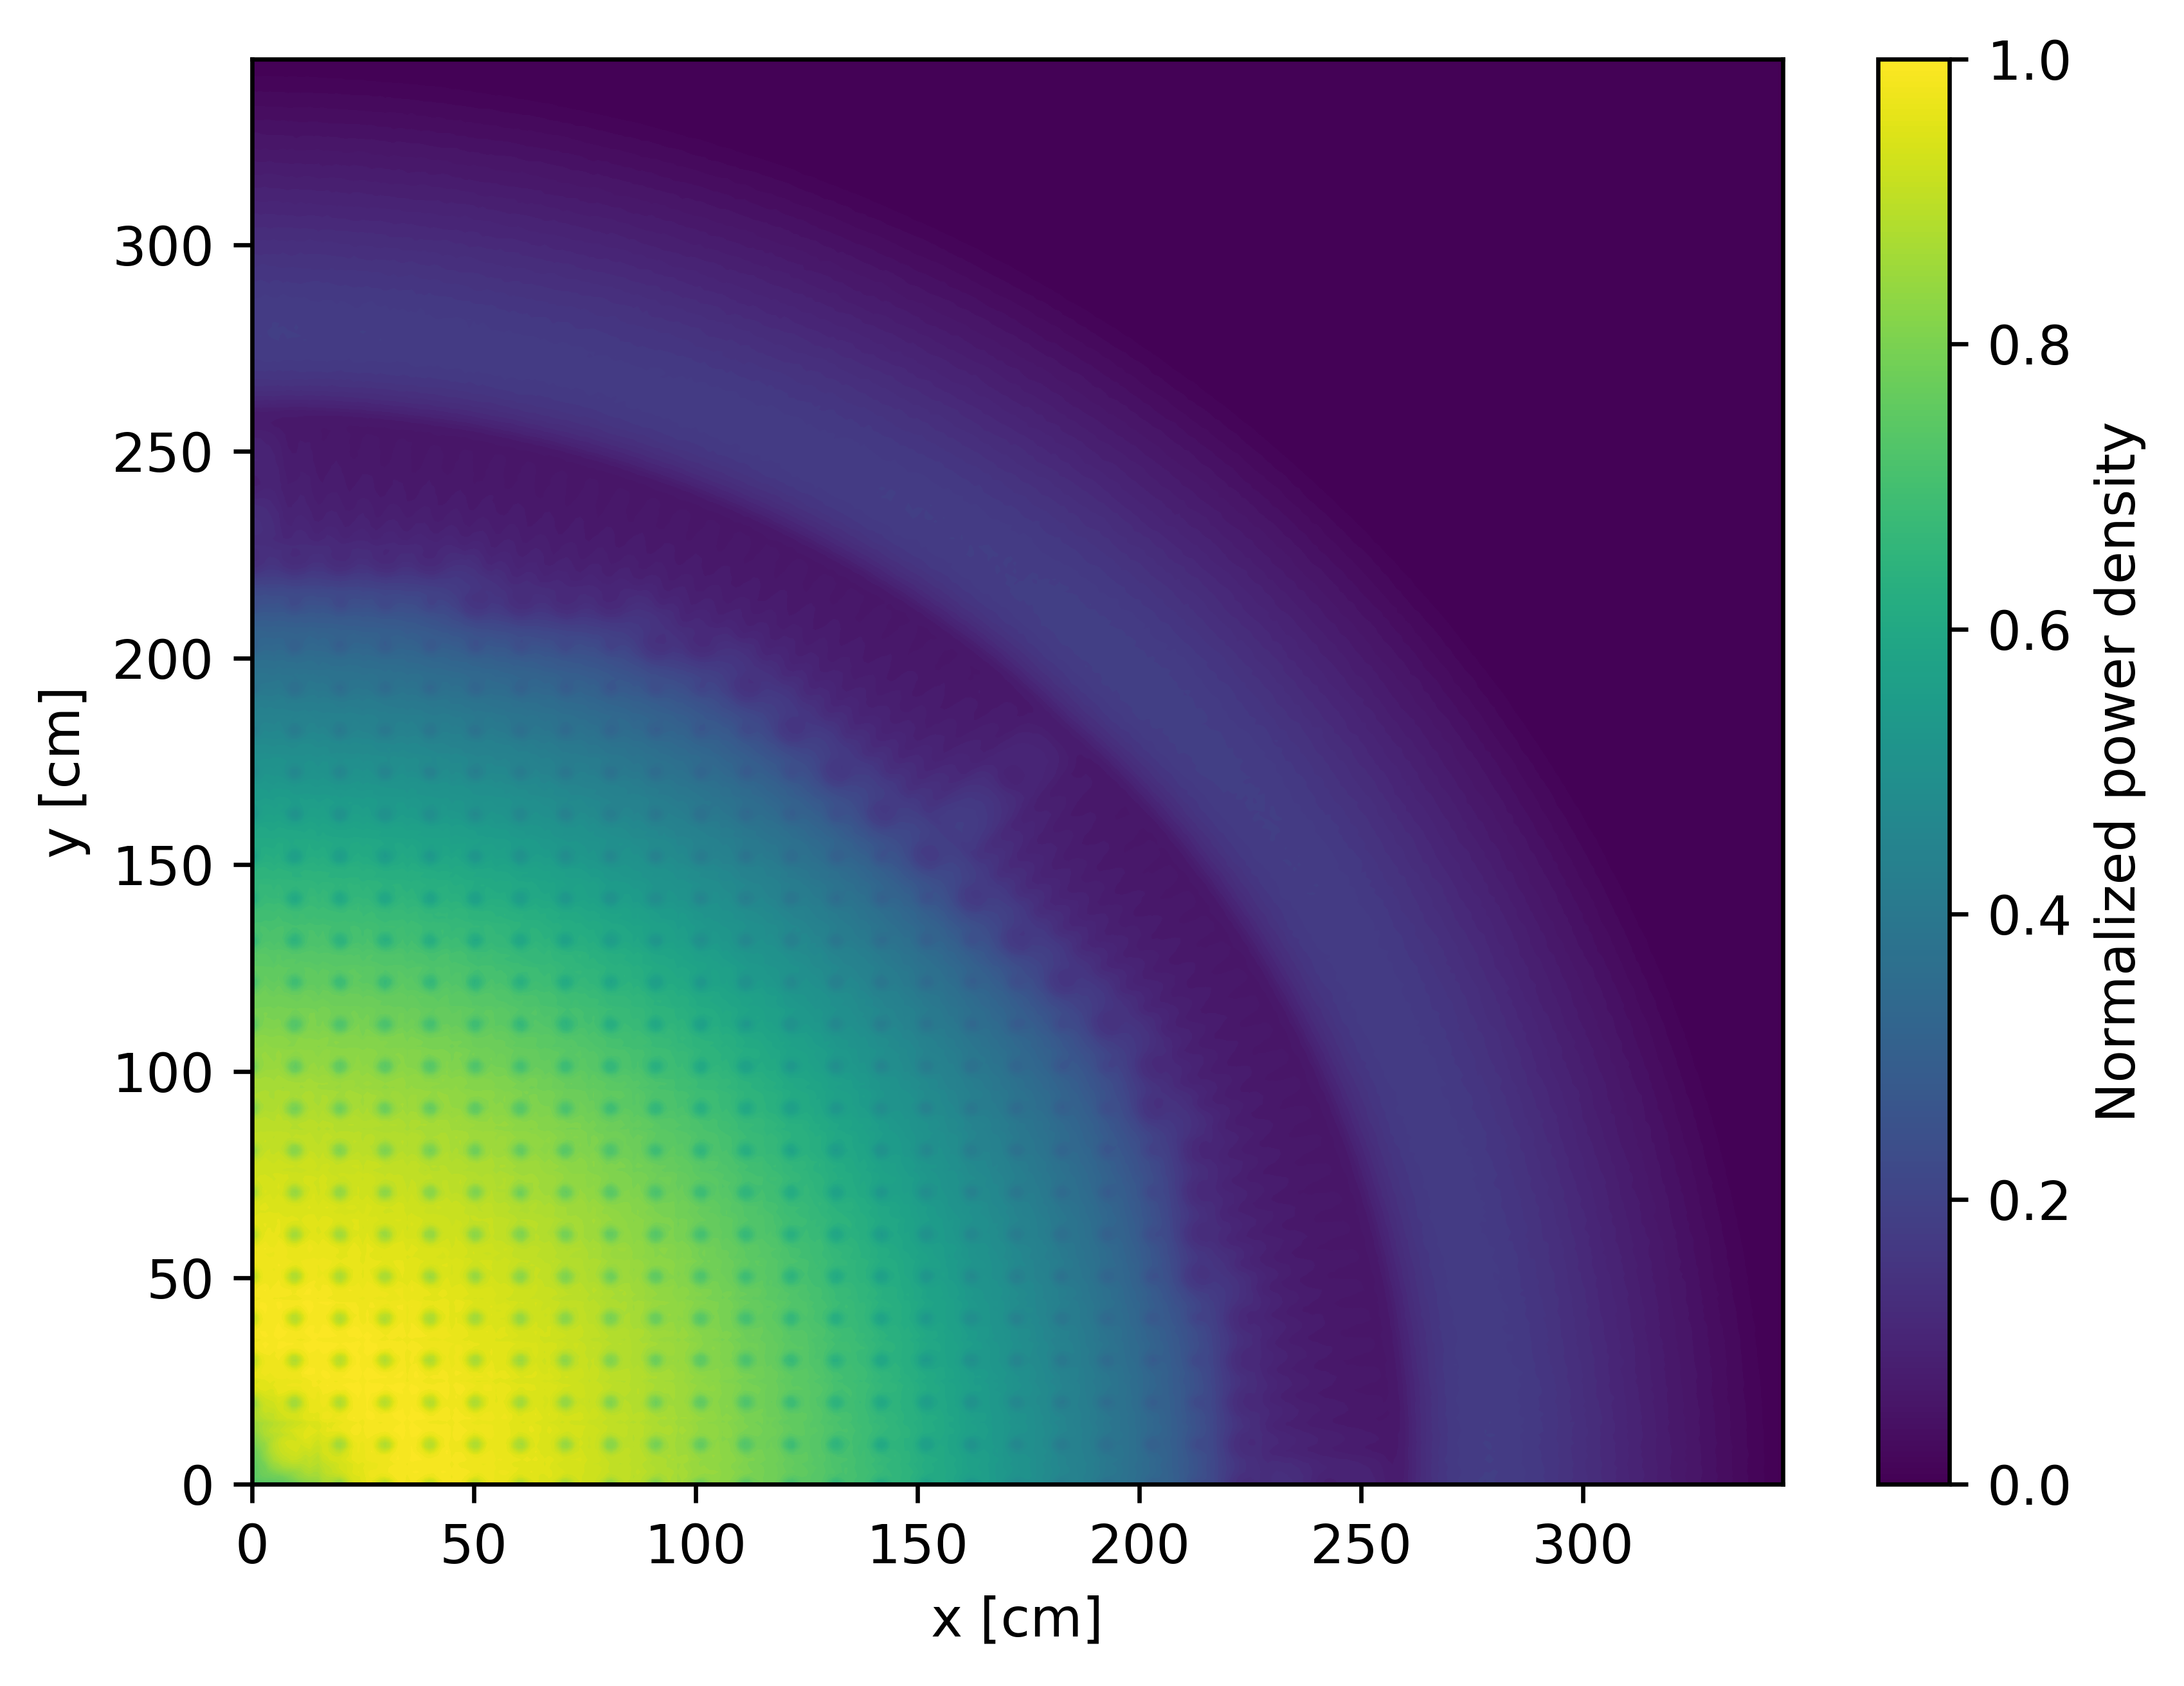
\includegraphics[width=0.82\textwidth]{ch3/power_distribution_eq.png} 
	\vspace{-5mm}
	\caption{Normalized power density for equilibrium fuel salt composition 
		(reproduced from Rykhlevskii \emph{et al.} 
		\cite{rykhlevskii_modeling_2019}).}
	\label{fig:pow_den}
\end{figure}

Figure~\ref{fig:breeding_den} shows the distribution of the neutron capture 
reaction rate for $^{232}$Th normalized by the total neutron flux for the 
initial and equilibrium states. The distribution reflects the spatial 
distribution of $^{233}$U production in the core. $^{232}$Th neutron capture 
produces $^{233}$Th, which then $\beta$-decays to $^{233}$Pa, the precursor 
for $^{233}$U production. Accordingly, this characteristic represents the 
breeding distribution in the \gls{MSBR} core. The power and breeding 
distribution remained almost constant during the reactor operation. Even after 
20 years of operation, most of the power is still generated in zone I.
\begin{figure}[ht!] % replace 't' with 'b' to force it to 
	\centering
	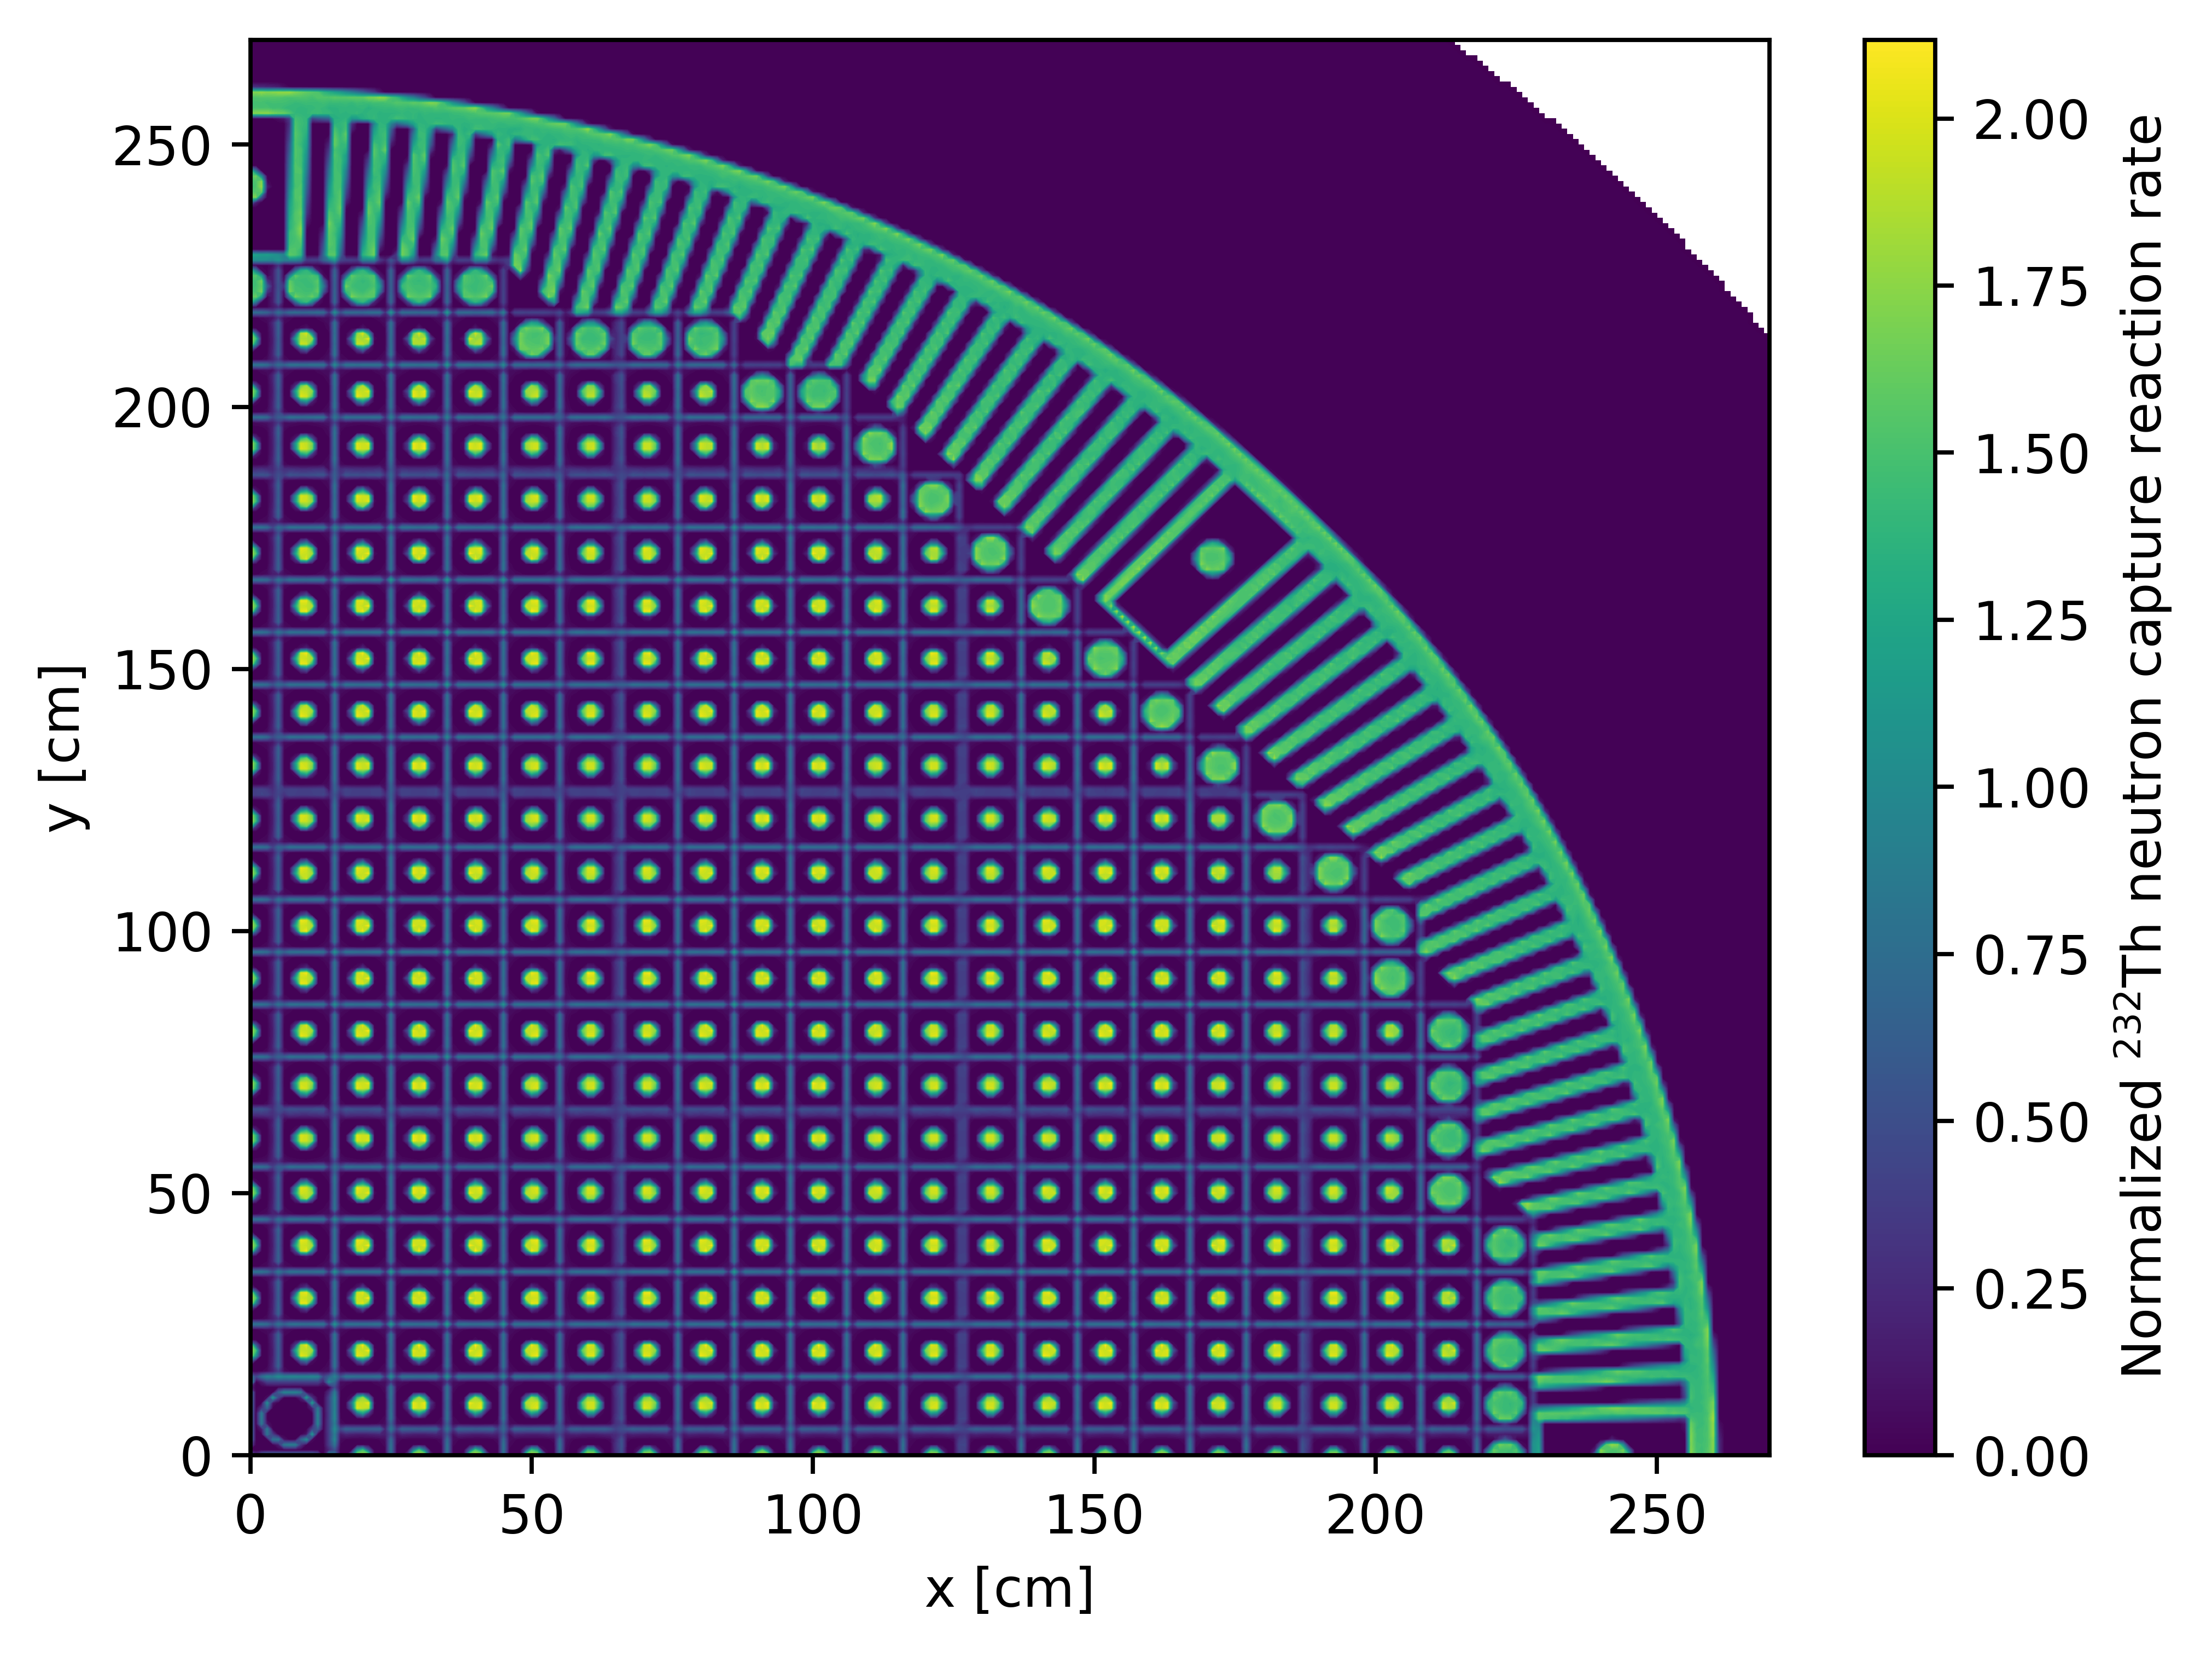
\includegraphics[width=0.82\textwidth]{ch3/breeding_distribution_eq.png} 
		\vspace{-5mm}
	\caption{$^{232}$Th neutron capture reaction rate normalized by total flux 
		for equilibrium fuel salt composition (reproduced from 
		Rykhlevskii \emph{et al.} \cite{rykhlevskii_modeling_2019}).}
	\label{fig:breeding_den}
\end{figure}
\FloatBarrier

%%%%%%%%%%%%%%%%%%%%%%%%%%%%%%%%%%%%%%%%%%%%%%%%%%%%%%%%%%%%%%%%%%%%%%%%%%%%%%%%
\subsection{Thorium refill rate}
In the \gls{MSBR}, the only external feed material flow  is $^{232}$Th. 
Figure~\ref{fig:th_refill} shows the $^{232}$Th feed rate calculated over 60 
years of reactor operation. The $^{232}$Th feed rate fluctuates significantly 
as a result of the batch-wise nature of this online reprocessing approach. 
Figure~\ref{fig:th_refill_zoomed} shows a zoomed thorium feed rate for a short 
150-EFPD interval. Note that the large spikes of up to 36 kg/day in a thorium 
consumption occur every 3435 days. Those spikes happened due to strong 
absorbers' (Rb, Sr, Cs, Ba) removal at the end of the effective cycle (100\% 
of these elements removing every 3435 days of operation). The corresponding 
effective multiplication factor increase (Figure~\ref{fig:keff}) and breeding  
intensification leads to additional $^{232}$Th consumption.  
\begin{figure}[ht!] % replace 't' with 'b' to force it to \centering
	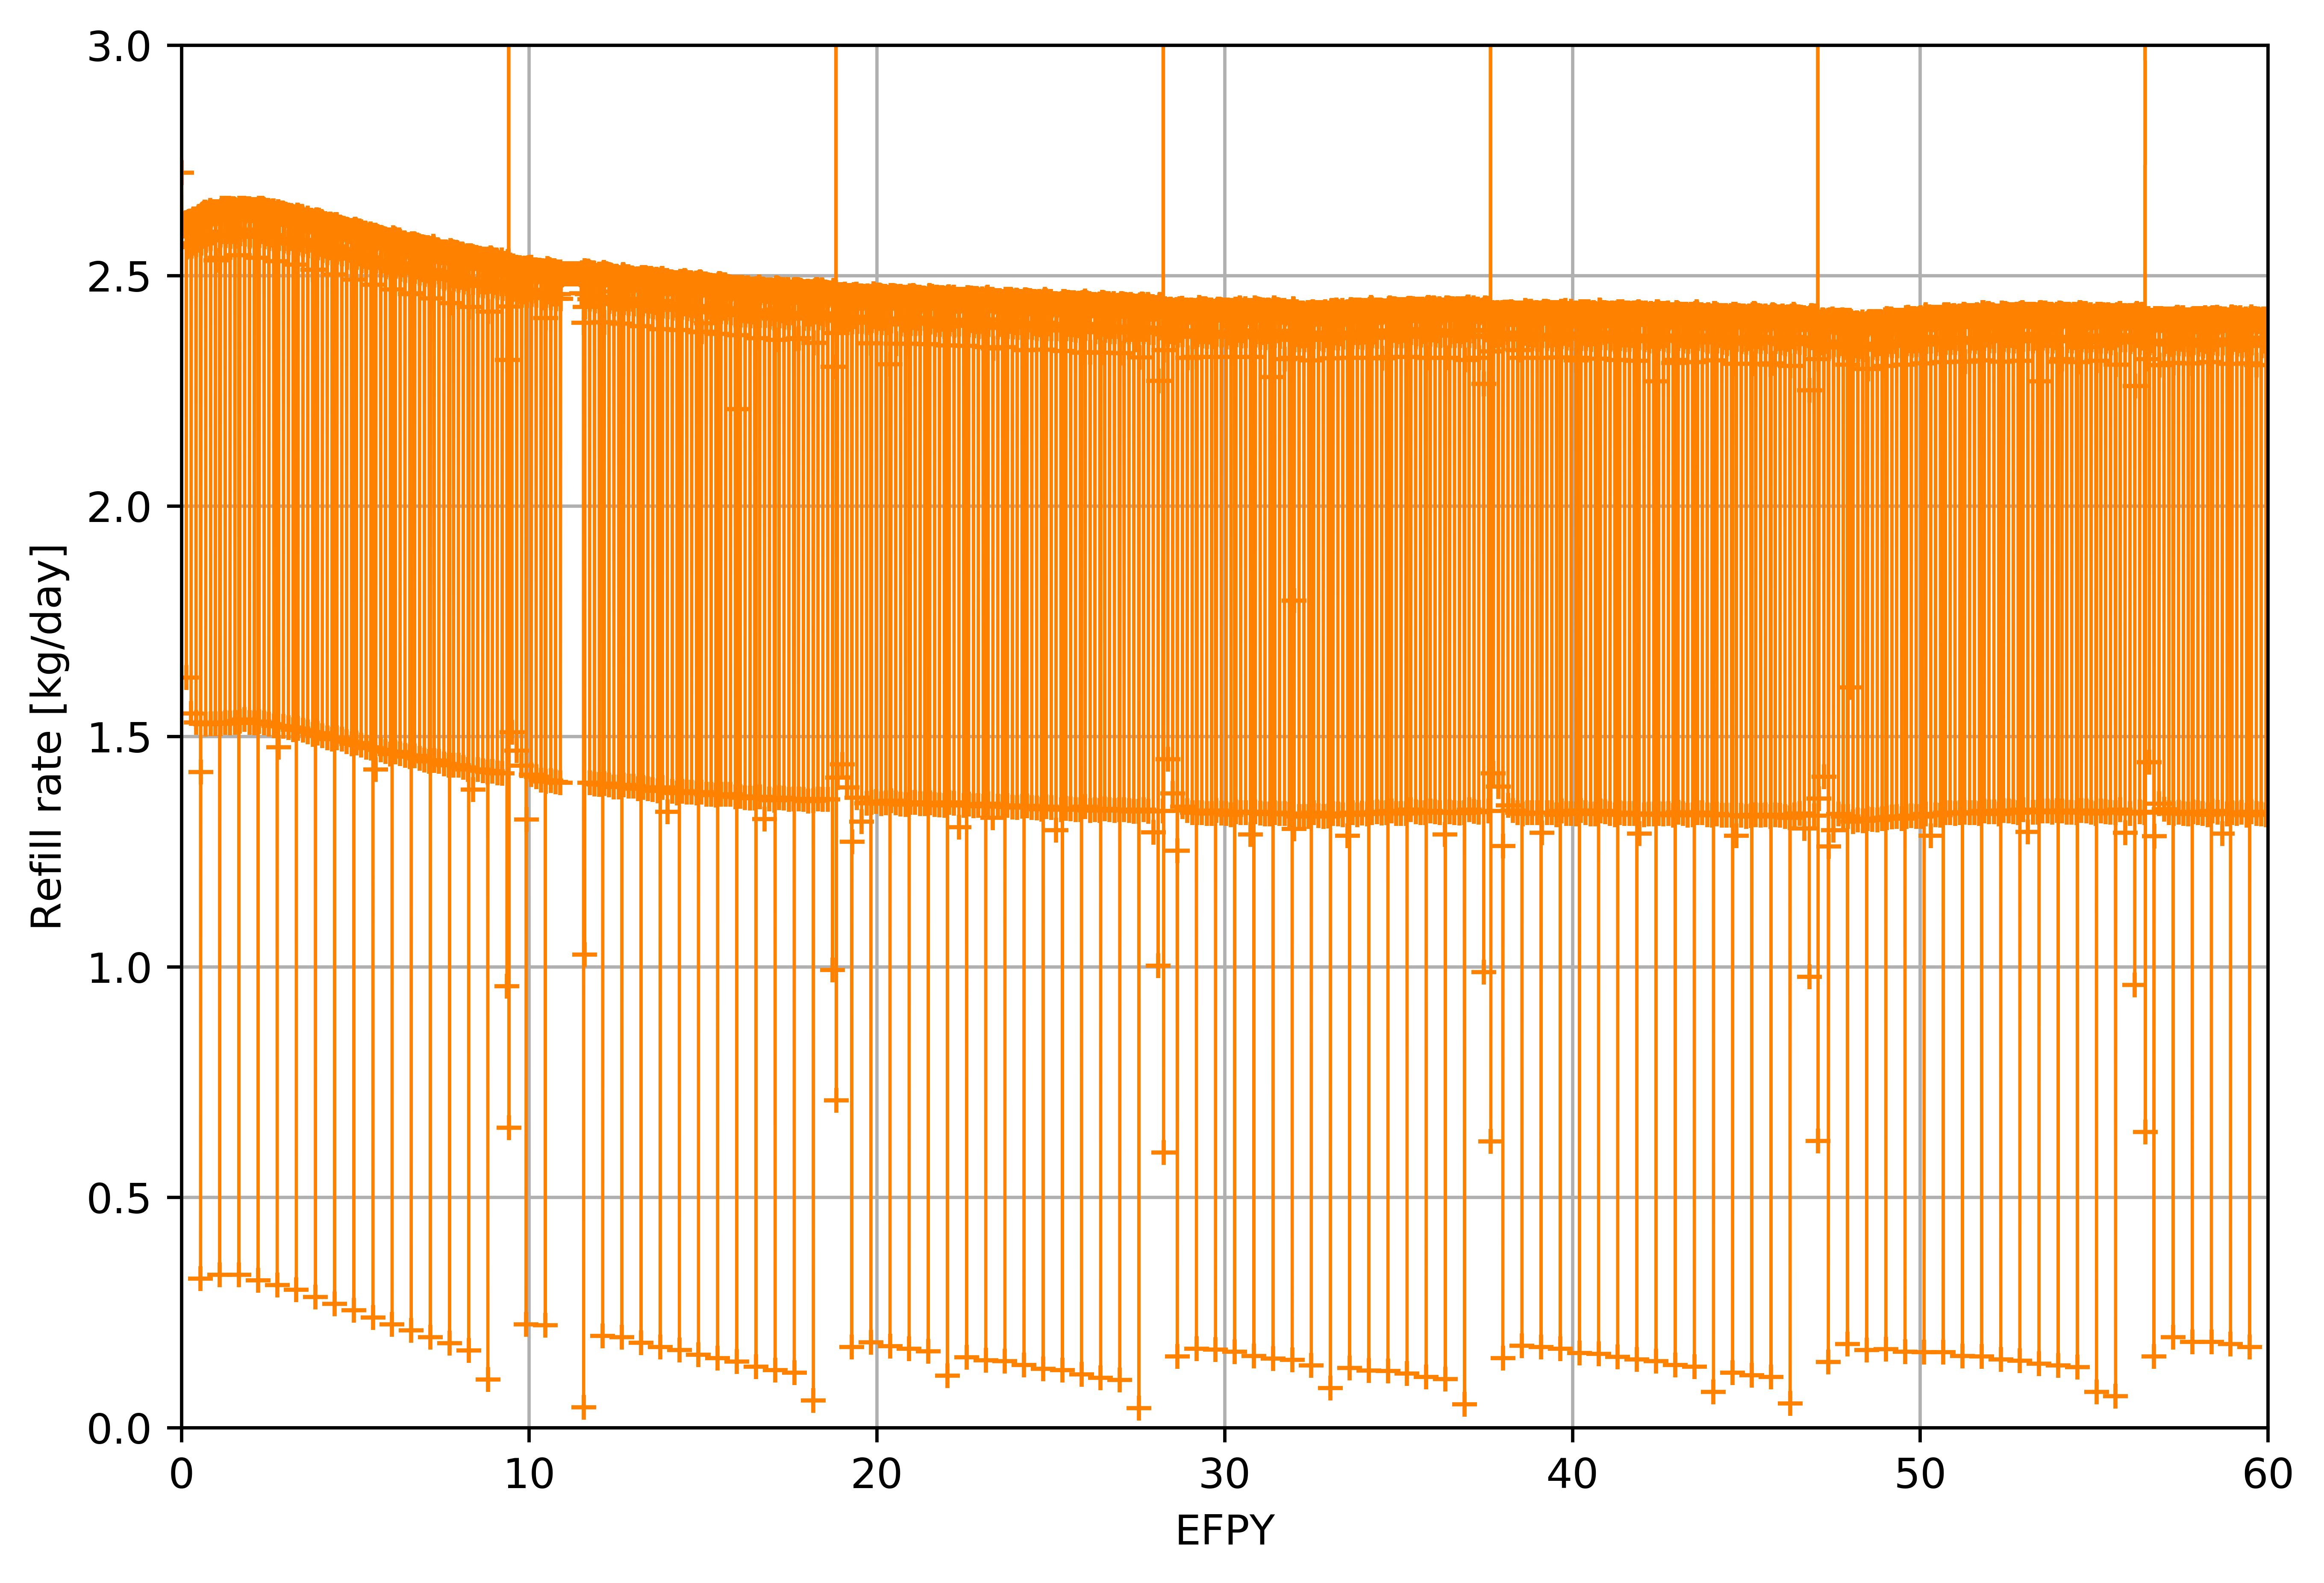
\includegraphics[width=\textwidth]{ch3/th_refill_rate.png} 
	\caption{$^{232}$Th feed rate over 60 years of the \gls{MSBR} operation 
	(reproduced from Rykhlevskii \emph{et al.} 
	\cite{rykhlevskii_modeling_2019}).}
	\label{fig:th_refill}
\end{figure}
\begin{figure}[ht!] % replace 't' with 'b' to force it to \centering
	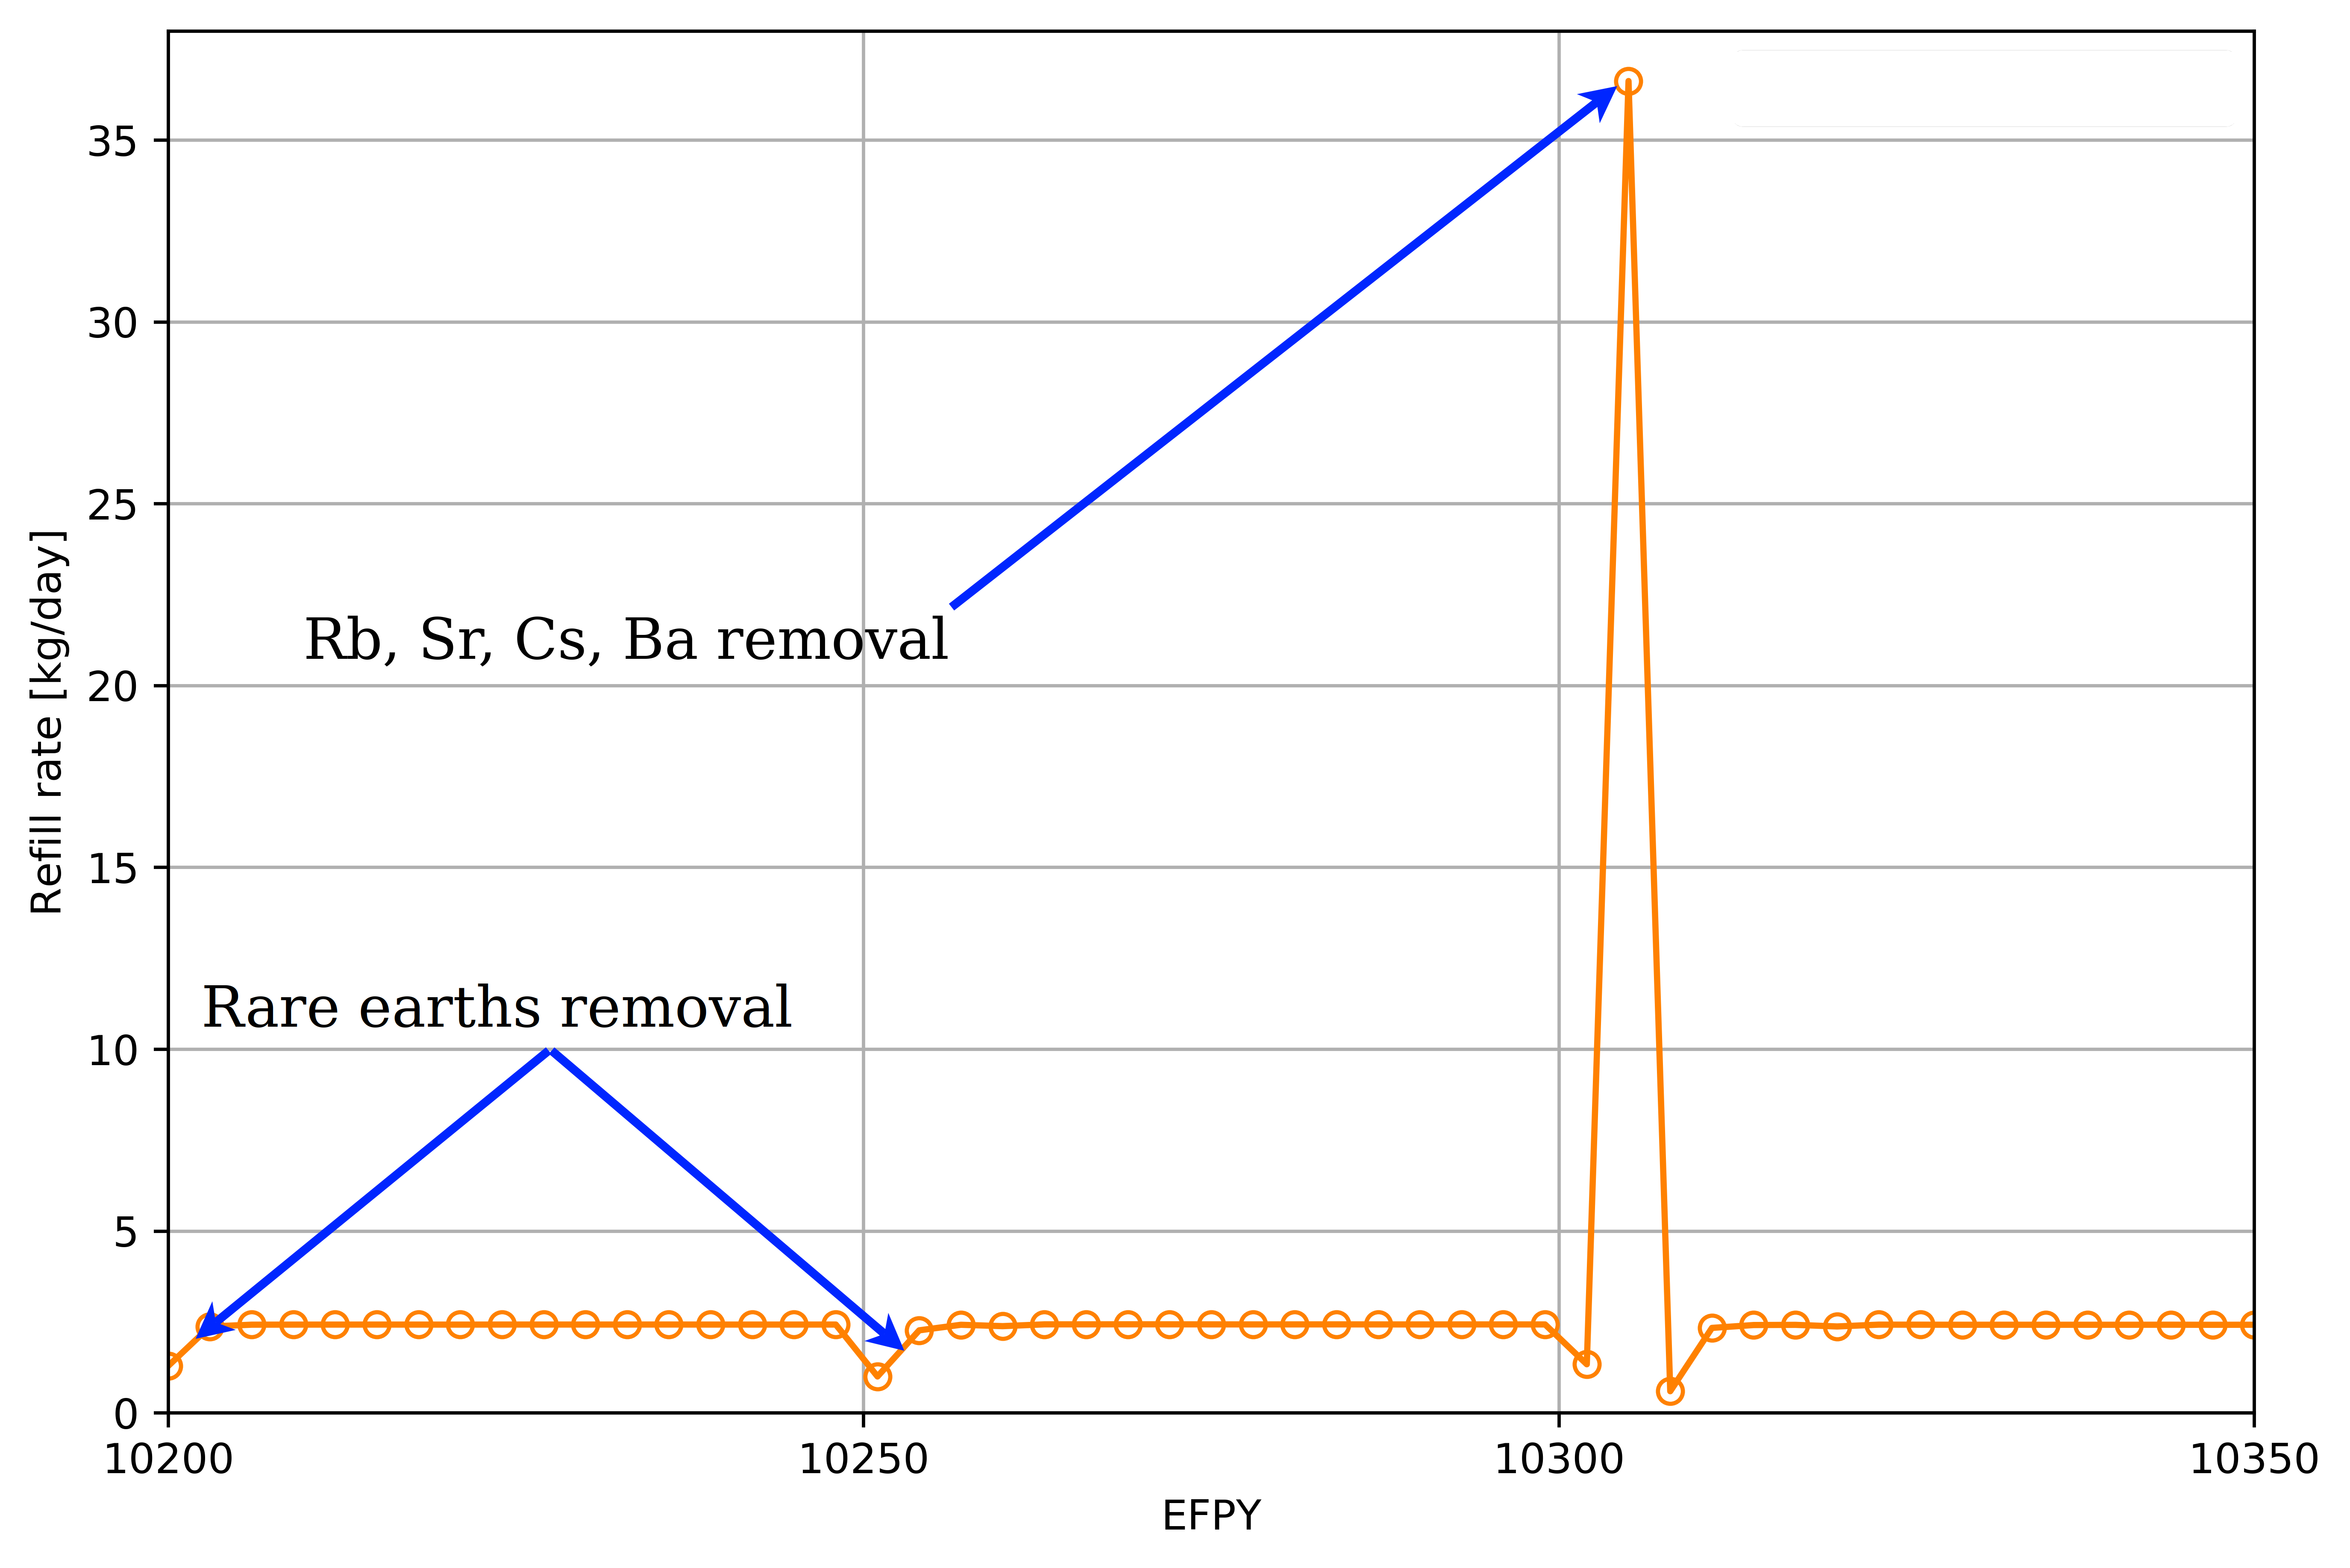
\includegraphics[width=\textwidth]{ch3/th_refill_rate_zoomed.png} 
	\caption{Zoomed $^{232}$Th feed rate for a 150-EFPD time interval 
	(reproduced from Rykhlevskii \emph{et al.} 
	\cite{rykhlevskii_modeling_2019}).}
	\label{fig:th_refill_zoomed}
\end{figure}

The average thorium feed rate increases during the first 500 days of operation 
and steadily decreases due to spectrum hardening and accumulation of absorbers 
in the core. As a result, the average $^{232}$Th feed rate over 60 years of 
operation is about 2.40 kg/day which is in a good agreement with a recent 
online reprocessing study by \gls{ORNL} (2.45 kg/day, 2\% difference) 
\cite{betzler_molten_2017, betzler_personal_2017}. At equilibrium, the thorium 
feed rate is determined by the reactor power, the energy released per fission, 
and the neutron energy spectrum.


\section{Operational and safety parameter evolution}
In Section~\ref{sec:equilibrium_search}, we reported how fuel salt composition 
changes during \gls{MSBR} operation. The number density of the most 
important heavy isotopes, $^{233}$U and $^{232}$Th, was stable while 
transitioning from startup to equilibrium composition  
(Figure~\ref{fig:adens_eq}). At the same time, a number of different 
actinides is being produced in the reactor core. Most of these nuclides 
($^{234}$U, $^{239}$Pu, $^{241}$Pu) have a much larger absorption cross 
section than $^{233}$U and $^{232}$Th loaded initially into the core, which 
causes significant neutron energy spectrum hardening. In the current section, 
we analyze how such neutron spectrum shift affects major operation and safety 
parameters such as temperature coefficients of reactivity and reactivity worth 
of the control rods. 

\subsection{Temperature coefficient of reactivity}
Table~\ref{tab:tcoef} summarizes temperature effects on reactivity calculated 
in this work for both initial and equilibrium fuel compositions, compared 
to the original \gls{ORNL} report data \cite{robertson_conceptual_1971}. 
By propagating the $k_{eff}$  statistical error provided by Serpent, 
uncertainty for each temperature coefficient was obtained and appears in 
Table~\ref{tab:tcoef}. Other sources of uncertainty are neglected, such as 
cross section measurement error and approximations inherent in the equations 
of state, providing both the salt and graphite density dependence on 
temperature. The main physical principle underlying the reactor temperature 
feedback is an expansion of heated material. If the fuel salt temperature 
increases, the density of the salt decreases; at the same time, the total 
volume of fuel salt in the core remains constant because the graphite bounds 
it. If the graphite temperature increases, the density of graphite 
decreases, creating additional space for fuel salt. To determine the 
temperature coefficients, the cross section temperatures for the fuel and 
moderator were changed from 900K to 1000K. Three different cases were 
considered:
\begin{enumerate}[itemsep=1pt,parsep=2pt]
	\item Temperature of fuel salt rising from 900K to 1000K.
	\item Temperature of graphite rising from 900K to 1000K.
	\item Whole reactor temperature rising from 900K to 1000K.
\end{enumerate}
%%%%%%%%%%%%%%%%%%%%%%%%%%%%%%%%%%%%%%%%
\begin{table}[ht!]
	\caption{Temperature coefficients of reactivity for the initial and 
	equilibrium states (reproduced from Rykhlevskii \emph{et al.} 
		\cite{rykhlevskii_modeling_2019}).}
	\begin{tabularx}{\textwidth}{ p{0.3\textwidth} R R R } \hline
		Reactivity coefficient   & Initial & Equilibrium  &  Reference
		\cite{robertson_conceptual_1971}                             \\ 
		& [pcm/K]         &  [pcm/K]        & (initial) [pcm/K] 
		\tabularnewline  \hline
		Doppler in fuel salt                    & $-4.73\pm0.038$ & 
		$-4.69\pm0.038$ & $-4.37$  \tabularnewline
		Fuel salt density                       & $+1.21\pm0.038$ & 
		$+1.66\pm0.038$ & $+1.09$  \tabularnewline
		Total fuel salt                         & $-3.42\pm0.038$ & 
		$-2.91\pm0.038$ & $-3.22$  \tabularnewline \hline
		Graphite spectral shift                 & $+1.56\pm0.038$ & 
		$+1.27\pm0.038$ &          \tabularnewline
		Graphite density                        & $+0.14\pm0.038$ & 
		$+0.23\pm0.038$ &          \tabularnewline
		Total moderator (graphite)              & $+1.69\pm0.038$ & 
		$+1.35\pm0.038$ & $+2.35$  \tabularnewline \hline
		Total core                              & $-1.64\pm0.038$ & 
		$-1.58\pm0.038$ & $-0.87$  \tabularnewline \hline
	\end{tabularx}
	\label{tab:tcoef}
\end{table}
%%%%%%%%%%%%%%%%%%%%%%%%%%%%%%%%%%%%%%%%%%%%%%%%%%%%%%%%%%%%%%%%%%%%%%%%%%%%%%%%
In the first case, changes in the fuel temperature only impact fuel density. 
In this case, the geometry is unchanged because the fuel is a liquid. However, 
if the moderator heats up, both the density and the geometry change due to 
the thermal expansion of the solid graphite blocks and reflector. Accordingly, 
the new graphite density was calculated using a linear temperature expansion 
coefficient of 1.3$\times10^{-6}$K$^{-1}$ \cite{robertson_conceptual_1971}. A 
new geometry input for Serpent, which takes into account the displacement of 
graphite surfaces, was created based on this information. For calculation of 
displacement, it was assumed that the interface between the graphite reflector 
and vessel is immobile and the vessel temperature is constant. This 
is the most reasonable assumption for the short-term reactivity effects 
because inlet salt cools the graphite reflector and the inner surface of the 
vessel.

The fuel temperature coefficient (FTC) is negative for both initial and 
equilibrium fuel compositions due to thermal Doppler broadening of the 
resonance capture cross sections in the thorium. A small positive effect of 
fuel density on reactivity increases from $+1.21$ pcm/K at reactor startup to 
$+1.66$ pcm/K for equilibrium fuel composition, which has a negative effect on 
FTC magnitude during the reactor operation; this is in good agreement with 
earlier research \cite{robertson_conceptual_1971,park_whole_2015}. The 
moderator temperature coefficient (MTC) is positive for the startup 
composition and decreases during reactor operation because of spectrum 
hardening with fuel depletion. Finally, the total temperature coefficient of 
reactivity is negative for both cases but decreases in magnitude during 
reactor operation due to spectral shift. In summary, even after 20 years of 
operation, the total temperature coefficient of reactivity is relatively large 
and negative during reactor operation (comparing with conventional PWR which 
has temperature coefficient about -1.71 pcm/$^\circ$F $\approx$ -3.08 pcm/K 
\cite{forget_integral_2018}), despite positive MTC, and affords excellent 
reactor stability and control.

\subsection{Reactivity control system rod worth}
Table~\ref{tab:rod_worth} summarizes the reactivity control system worth. 
During normal operation, the control (graphite) rods are fully inserted, and 
the safety (B$_4$C) rods are fully withdrawn. To insert negative reactivity 
into the core, the graphite rods are gradually withdrawn from the core. In an 
accident, the safety rods would be dropped down into the core. The integral 
rod worths were calculated for various positions to separately estimate the 
worth of graphite control rods, the emergency shutdown rods, and the whole 
reactivity control system. Control rod integral worth is approximately 28 
cents and stays almost constant during reactor operation. The emergency 
shutdown rod integral worth decreases by 16.2\% during 20 years of operation 
because of neutron spectrum hardening and absorber accumulation in proximity 
to reactivity control system rods. This 16\% decline in control system worth 
must be taken into account in \gls{MSBR} 
accident analysis and safety justification.
%%%%%%%%%%%%%%%%%%%%%%%%%%%%%%%%%%%%%%%%
\begin{table}[ht!]
	\caption{Control system rod worth for the initial and equilibrium fuel 
		compositions (reproduced from Rykhlevskii \emph{et al.} 
		\cite{rykhlevskii_modeling_2019}).}
	\begin{tabularx}{\textwidth}{ p{0.5\textwidth}  R  R } \hline
		Reactivity parameter  &  Initial[\cent]    &  Equilibrium[\cent]  \\ 
		\hline
		Graphite control rod integral worth               & $\ 28.2\pm0.8$    
		& $\ 
		29.0\pm0.8$ \\ Emergency shutdown rod integral worth                  
		& 
		$251.8\pm0.8$    & $211.0\pm0.8$  \\
		Total reactivity control system worth               & $505.8\pm0.7$    
		& 
		$424.9\pm0.8$ \\ \hline
	\end{tabularx}
	\label{tab:rod_worth}
\end{table}
%%%%%%%%%%%%%%%%%%%%%%%%%%%%%%%%%%%%%%%%%%%%%%%%%%%%%%%%%%%%%%%%%%%%%%%%%%%%%%%%

\subsection{Six Factor Analysis}
The effective multiplication factor can be expressed using the following 
formula:
\begin{align}
k_{eff} &=  \eta f p \epsilon P_f P_t
\intertext{where}
\eta     &= \mbox{neutron reproduction factor $[-]$}  \nonumber \\
f        &= \mbox{thermal utilization factor $[-]$}   \nonumber \\
p        &= \mbox{resonance escape probability $[-]$} \nonumber \\
\epsilon &= \mbox{fast fission factor $[-]$}          \nonumber \\
P_f      &= \mbox{fast non-leakage probability $[-]$} \nonumber \\
P_t      &= \mbox{thermal non-leakage probability $[-]$.} \nonumber
\end{align}

Table~\ref{tab:six_factor} summarizes the six factors for both the initial and 
equilibrium fuel salt compositions. Using Serpent and SaltProc, these factors 
and their statistical uncertainties have been calculated for both the initial 
and equilibrium fuel salt compositions (see Table~\ref{tab:msbr_tab}). The 
fast and thermal non-leakage probabilities remain constant despite the 
evolving neutron spectrum during operation. In contrast, the neutron 
reproduction factor ($\eta$), resonance escape probability ($p$), and fast 
fission factor ($\epsilon$) are considerably different between startup and 
equilibrium. As indicated in Figure~\ref{fig:spectrum}, the neutron spectrum 
is softer at the beginning of reactor life. Neutron spectrum hardening causes 
the fast fission factor to increase through the core lifetime; the opposite is 
true for the resonance escape probability. Finally, the neutron reproduction 
factor decreases during reactor operation due to the accumulation of fissile 
plutonium isotopes.
%%%%%%%%%%%%%%%%%%%%%%%%%%%%%%%%%%%%%%%%
\begin{table}[hb!]
	\caption{Six factors for the full-core \gls{MSBR} model for the initial 
	and equilibrium fuel compositions (reproduced from Rykhlevskii \emph{et 
		al.} \cite{rykhlevskii_modeling_2019}).}
	\begin{tabularx}{\textwidth}{ p{0.5\textwidth}  R  R } \hline
		Factor  & Initial      & Equilibrium   \\ \hline
		Neutron reproduction factor ($\eta$)     & $1.3960\pm.000052$     & 
		$1.3778\pm.00005$ \\ Thermal utilization factor (f)           & 
		$0.9670\pm.000011$     & $0.9706\pm.00001$ \\
		Resonance escape probability (p)         & $0.6044\pm.000039$     & 
		$0.5761\pm.00004$ \\
		Fast fission factor ($\epsilon$)         & $1.3421\pm.000040$     & 
		$1.3609\pm.00004$ \\
		Fast non-leakage probability (P$_f$)     & $0.9999\pm.000004$     & 
		$0.9999\pm.000004$ \\
		Thermal non-leakage probability (P$_t$)  & $0.9894\pm.000005$     & 
		$0.9912\pm.00005$ \\ \hline
	\end{tabularx}
	\label{tab:six_factor}
\end{table}

\section{Benefits of fission products removal}
To investigate how online fuel salt processing described in Chapter 2 affects 
the reactor performance, the separate effect of each poison group removal 
was studied in this section.

\subsection{The effect of removing fission products from the fuel salt}
Loading the initial fuel salt composition into the \gls{MSBR} core leads to a 
supercritical configuration (Figure~\ref{fig:fp_removal}). After reactor 
startup, the effective multiplication factor for the case with volatile gases 
and noble metals removal is approximately 7500 pcm  higher than for the case 
without fission product removal. This significant impact on the reactor core 
lifetime is achieved due to the immediate removal (20 sec cycle time) and the 
high absorption cross sections of Xe, Kr, Mo, and other noble metals removed. 
The effect of rare earth element removal is significant in a few months after 
startup and reached approximately 5500 pcm after 10 years of operation. The 
rare earth elements were removed at a slower rate (50-day cycle time). 
Moreover, Figure~\ref{fig:fp_removal} demonstrates that batch-wise removal of 
strong absorbers every 3 days unnecessarily leads to fluctuation in results, 
but rare earth element removal every 50 days causes an approximately 600 pcm 
jump in reactivity.
\begin{figure}[ht!] % replace 't' with 'b' to force it to 
	\centering
	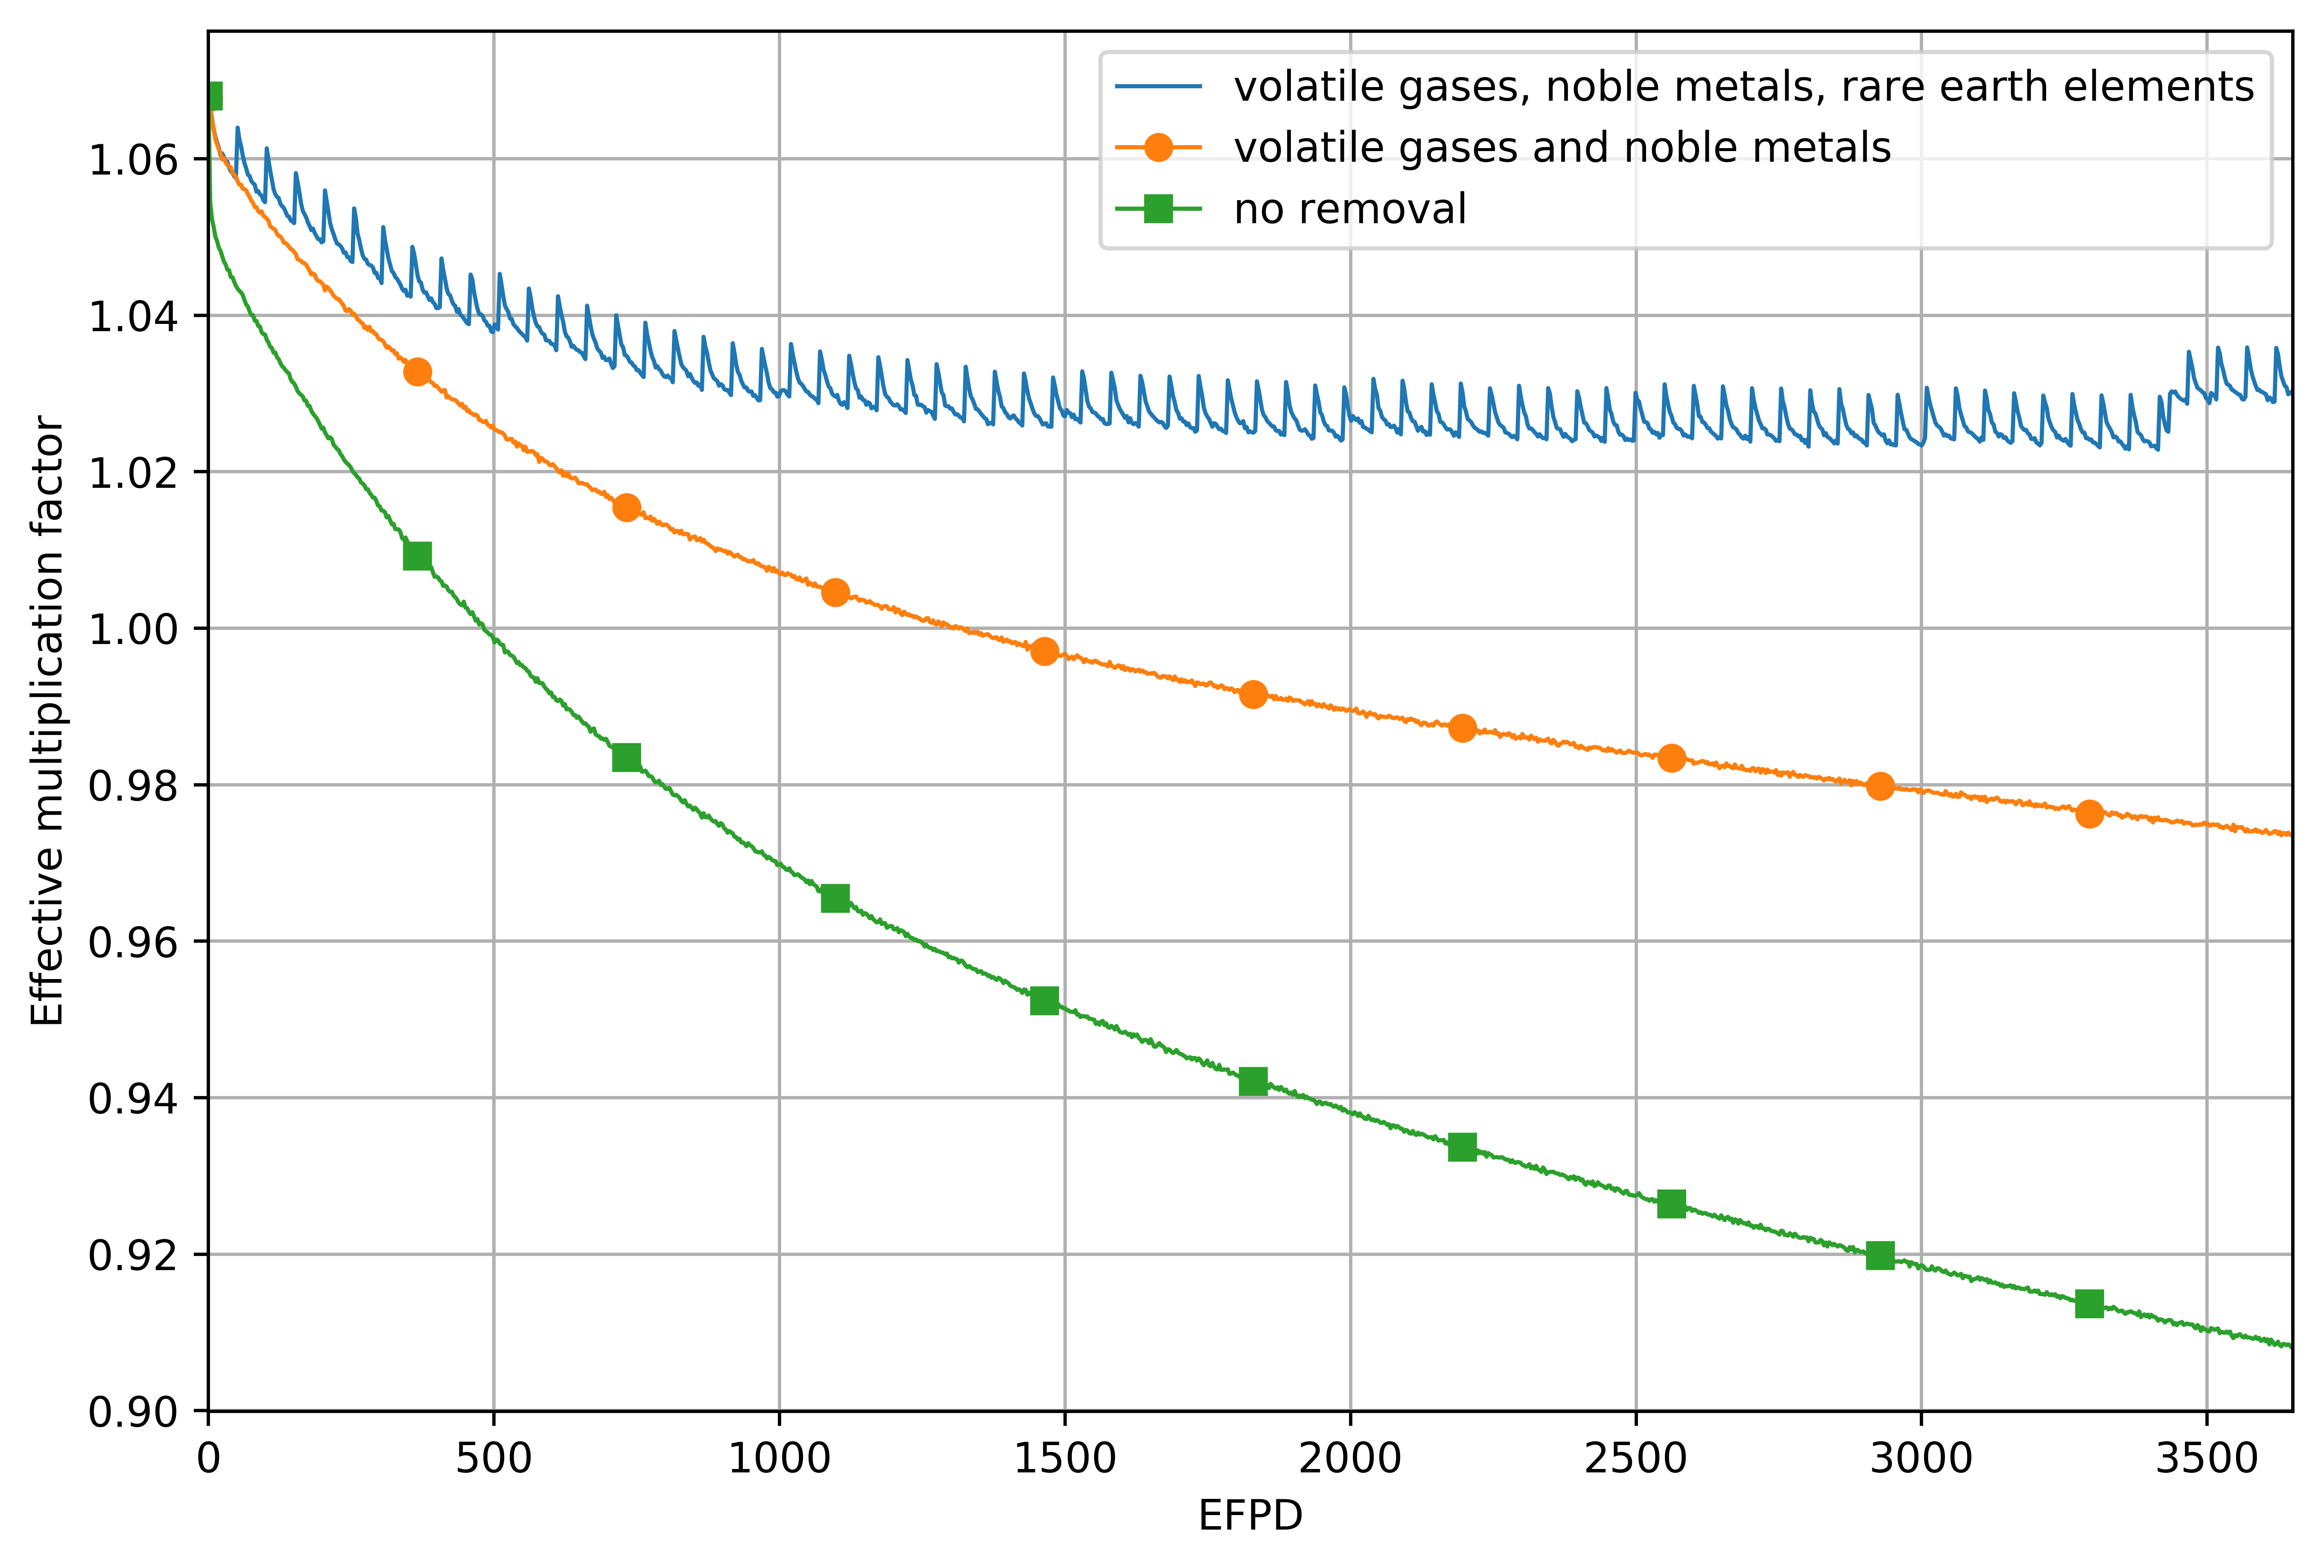
\includegraphics[width=\textwidth]{ch3/keff_rem_cases.png} 
	\caption{Calculated effective multiplication factor for the full-core 
		\gls{MSBR} model with the removal of various fission product groups 
		over 10 years of operation (reproduced from Rykhlevskii \emph{et al.} 
		\cite{rykhlevskii_modeling_2019}).}
	\label{fig:fp_removal}
\end{figure}

The effective multiplication factor of the core reduces gradually over 
operation time because the fissile material ($^{233}$U) continuously depletes 
from the fuel salt due to fission while fission products accumulate in the 
fuel salt simultaneously. Eventually, without fission products removal, the 
reactivity decreases to the subcritical state after approximately 500 and 
1300 days of operation for cases with no removal and volatile gases \& noble 
metals removal, respectively. The time when the simulated core becomes  
subcritical ($k_{eff}<$1.0 for full-core model) is called the core 
lifetime. Therefore, removing fission products provides significant 
neutronic benefits and enables a longer core lifetime.


\section{Concluding remarks}

This chapter introduces the first ever version of the open-source \gls{MSR} 
simulation package SaltProc v0.1. The main goal of this work has been to 
demonstrate SaltProc's capability to find the equilibrium fuel salt 
composition (the number densities of major isotopes vary by less than 1\% over 
several years). A secondary goal has been to compare predicted operational and 
safety parameters (e.g., neutron energy spectrum, power and breeding 
distribution, temperature coefficients of reactivity) of the \gls{MSBR} at 
startup and equilibrium states. A tertiary goal has been to demonstrate the 
benefits of continuous fission product removal for thermal \gls{MSR} design.

To achieve these goals, a full-core high-fidelity benchmark model of the 
\gls{MSBR} was created in Serpent 2. The full-core model was used instead of 
the simplified single-cell model \cite{betzler_molten_2017, 	
rykhlevskii_online_2017, betzler_fuel_2018} to precisely describe the 
two-region \gls{MSBR} concept design sufficiently to represent breeding in the 
outer core zone accurately. When running depletion calculations, the most 
critical fission products and $^{233}$Pa are removed, while fertile and  
fissile materials are added to the fuel salt every 3 days.  Meanwhile, the 
removal interval for the rare earths, volatile fluorides, and semi-noble 
metals was greater than one month (50 days), which caused significant 
$k_{eff}$  
fluctuation. 

The results in this chapter indicate that $k_{eff}$ slowly decreases from 
1.075 and reaches 1.02 at equilibrium after approximately 6 years of 
operation. At the same time, the concentrations of $^{233}$U, $^{232}$Th, 
$^{233}$Pa, and $^{232}$Pa stabilized after approximately 2500 days of 
operation. Particularly, $^{233}$U number density 
equilibrates\footnote{fluctuates less than 0.8\%} after 16 years of operation. 
Consequently, the core reaches the quasi-equilibrium state after 16 years of 
operation. However, a wide variety of actinides, including fissile isotopes 
(e.g., $^{233}$U and $^{239}$Pu) and non-fissile strong absorbers ($^{234}$U), 
continue accumulating in the core. 

Those actinides cause neutron energy spectrum hardening as the core  
approaches equilibrium. Moreover, the neutron energy spectrum in the central 
core region is much softer than in the outer core region due to the lower 
moderator-to-fuel ratio in the outer zone, and this distribution remains 
stable during reactor operation. Finally, the epithermal or thermal spectrum 
is needed to effectively breed $^{233}$U from $^{232}$Th because the radiative 
capture cross section of $^{232}$Th monotonically decreases from $10^{-10}$ 
MeV to $10^{-5}$ MeV. A harder spectrum in the outer core region tends to 
significantly increase resonance absorption in thorium and decrease the 
absorption in fissile and structural materials. 

The spatial power distribution in the \gls{MSBR} shows that 98\% of the 
fission power is generated in the central zone I, and the neutron energy 
spectral shift has zero effect on the power distribution. The 
spatial distribution of neutron capture reaction rate for fertile $^{232}$Th, 
corresponding to breeding in the core, confirms that most of the breeding 
occurs in an outer, undermoderated, region of the \gls{MSBR} core. Finally, 
the average $^{232}$Th refill rate throughout 60 years of operation is 
approximately 2.40 kg/day or 100 g/GWh$_e$.

We compared the safety parameters at startup and equilibrium state using the 
Serpent Monte Carlo code. The total temperature coefficient is large and 
negative at startup 
and equilibrium, but the magnitude decreases throughout reactor operation from 
$-1.64$ to $-1.58$ pcm/K as the spectrum hardens. The moderator temperature 
coefficient is positive and also decreases during fuel depletion. The 
reactivity control system efficiency analysis showed that the safety rod 
integral worth decreases by approximately 16.2\% over 16 years of operation, 
while the graphite rod integral worth remains constant. Therefore, neutron 
energy spectrum hardening during fuel salt depletion has an undesirable impact 
on \gls{MSBR} stability and controllability and should be taken into  
consideration in further analysis of transient accident scenarios.

Finally, we proved that the \gls{MSBR} core performance benefits from the 
removal of volatile gases, noble metals, and rare earths from the fuel salt. 
Immediate removal of volatile gases (e.g., xenon) and noble metals 
increased reactivity by approximately 7500 pcm over a 10-year timeframe. In 
contrast, the effect of relatively slower removal of rare earth elements 
(every 50 days cycle instead of 3 days) has less impact (5500 pcm) on the core 
reactivity after 10 years of operation. An additional study is needed to 
establish neutronic  and economic tradeoffs of removing each element.

This chapter's results also helped identify the main directions of SaltProc 
v0.1 improvement. Firstly, the poison removal efficiency is not ideal, as was 
discussed in Chapter 1; consequently, the user should be able to simulate the 
fuel salt reprocessing system using a variable, non-ideal extraction 
efficiency. Secondly, SaltProc v0.1 entirely removes elements with longer 
residence times (semi-noble metals, volatile fluorides, Rb, Sr, Cs, Ba, Eu) at 
the end of cycle time (e.g., 3435 days for rubidium) which causes significant  
jumps in $k_{eff}$ due to the removal of large batches of the poison at once. 
In SaltProc v1.0, this drawback has been eliminated by removing a fraction of 
the target element with longer residence time at each depletion step. In the 
following chapters, improved SaltProc v1.0 capabilities will be demonstrated.
\chapter{Tool demonstration: Transatomic Power MSR}

In this chapter, I demonstrate SaltProc v1.0 capabilities for the \gls{TAP} 
\gls{MSR}. The \gls{TAP} concept was selected because it is well analyzed in 
the literature \cite{betzler_two-dimensional_2017, betzler_assessment_2017-1};
thus, code-to-code verification with ChemTRITON/SCALE is possible 
\cite{betzler_assessment_2017-1}. The demonstration was performed for two 
timescales:
\paragraph{Long-term.} I performed the \gls{TAP} \gls{MSR} core lifetime-long 
(25 years) depletion simulation with moderate time resolution (3-day depletion 
step) and constant, 100\% power level. The 
results obtained with SaltProc v1.0 are compared with recent efforts discussed 
in Chapter 1, more specifically with full-core \gls{TAP} depletion analysis 
with ideal removal efficiencies by Betzler \emph{et al.}  
\cite{betzler_assessment_2017-1}. This validation effort showed that SaltProc 
v1.0 solution is correct for the case with \emph{ideal extraction efficiency}.
\paragraph{Short-term (transient).} I performed the 24-hour-long depletion 
simulation with changing, load following reactor power with the fine time 
resolution (variable depletion step from 1 to 30-min). The depletion 
calculation for the \gls{TAP} in load following regime capture the effects of 
xenon poisoning and evaluate the benefit of using an online gas removal system.

In this chapter, I also analyze the reactor load-following capability for 
various moderator configurations and fuel salt compositions to bound design 
parameters of gas removal system to ensure load-following operation. 

\section{Transatomic Power Molten Salt Reactor concept design and model  
description}

The \gls{TAP} concept is a 1250 MW$_{th}$ \gls{MSR} with a LiF-based uranium 
fuel salt \cite{transatomic_power_corporation_technical_2016}. This concept 
uses configurable zirconium hydride rods as the moderator while most \gls{MSR} 
designs typically propose high-density reactor graphite. Zirconium hydride 
offers a much higher neutron moderating density than graphite: much less 
zirconium hydride volume is needed to achieve a thermal energy spectrum 
similar to one obtained with graphite moderator. Moreover, zirconium hydride 
has a much longer lifespan in extreme operational conditions (high 
temperature, large neutron flux, chemically aggressive salt) than reactor 
graphite. Finally, zirconium hydride is a nonporous material and holds up 
fewer neutron poisons (e.g., xenon, krypton) than does high-density 
reactor graphite.

In this section, the design characteristics and reprocessing plant design are 
based on information presented in the TAP white papers  
\cite{transatomic_power_corporation_technical_2016,
transatomic_power_corporation_neutronics_2016} and \gls{ORNL} technical 
reports \cite{betzler_two-dimensional_2017, betzler_assessment_2017-1}.

\subsection{TAP design description}

Figure~\ref{fig:tap-rendering} demonstrates a rendering of the primary and 
secondary loop of the \gls{TAP} \gls{MSR} seated inside a concrete nuclear 
island. Figure~\ref{fig:tap-primary-scheme} shows the schematic design of a 
520 MW$_{e}$, 2-loop nuclear reactor system with an intermediate salt loop.
\begin{figure}[h] % replace 't' with 'b' to 
	\centering
	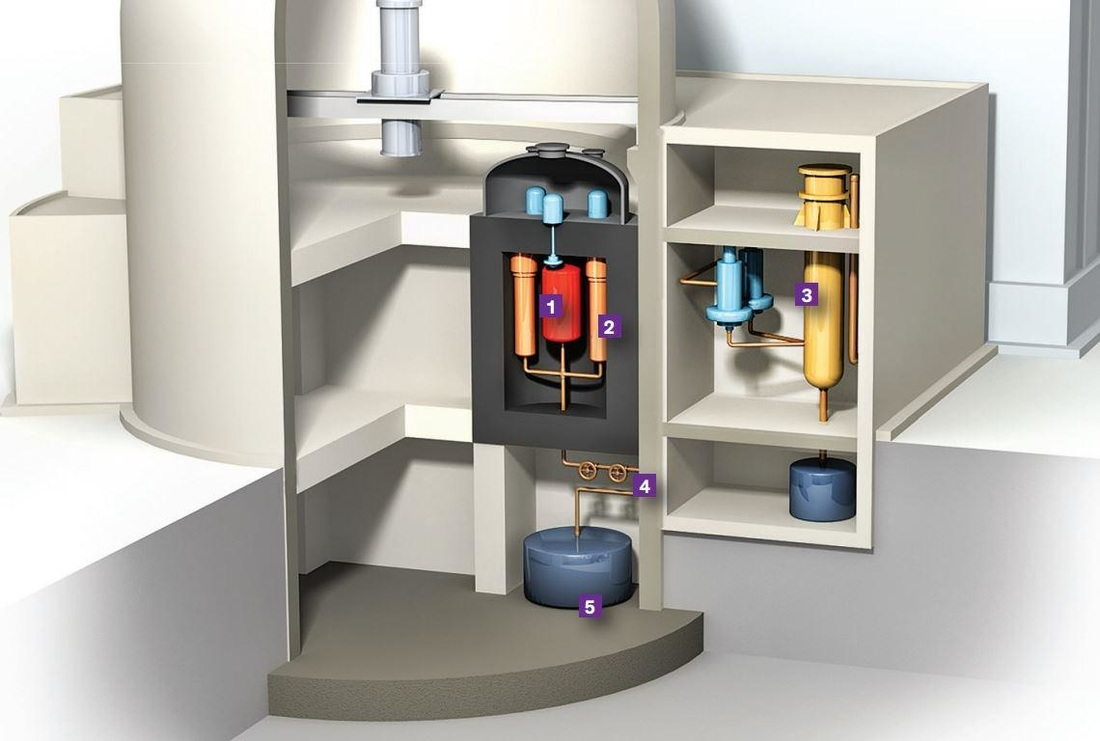
\includegraphics[width=\textwidth]{ch4/tap_render.jpg}
	\caption{Rendering of the \gls{TAP} \gls{MSR}. The fission happens in the 
		fuel salt inside the reactor vessel (1). The heat generated by 
		self-sustaining nuclear fission reaction would be transferred to the 
		secondary salt by heat exchanger (2), which would boil water in the 
		steam 
		generator (3). Valves made of salt with higher melting point (4) would 
		melt in case of emergency, allowing the salt to drain into a drain 
		tank 
		(5) which is able to passively dissipate decay heat	(reproduced from 
		\cite{strickland_transatomic_2014}, illustration by Emily Cooper).}
	\label{fig:tap-rendering}
\end{figure}
\begin{figure}[h] % replace 't' with 'b' to 
	\centering
	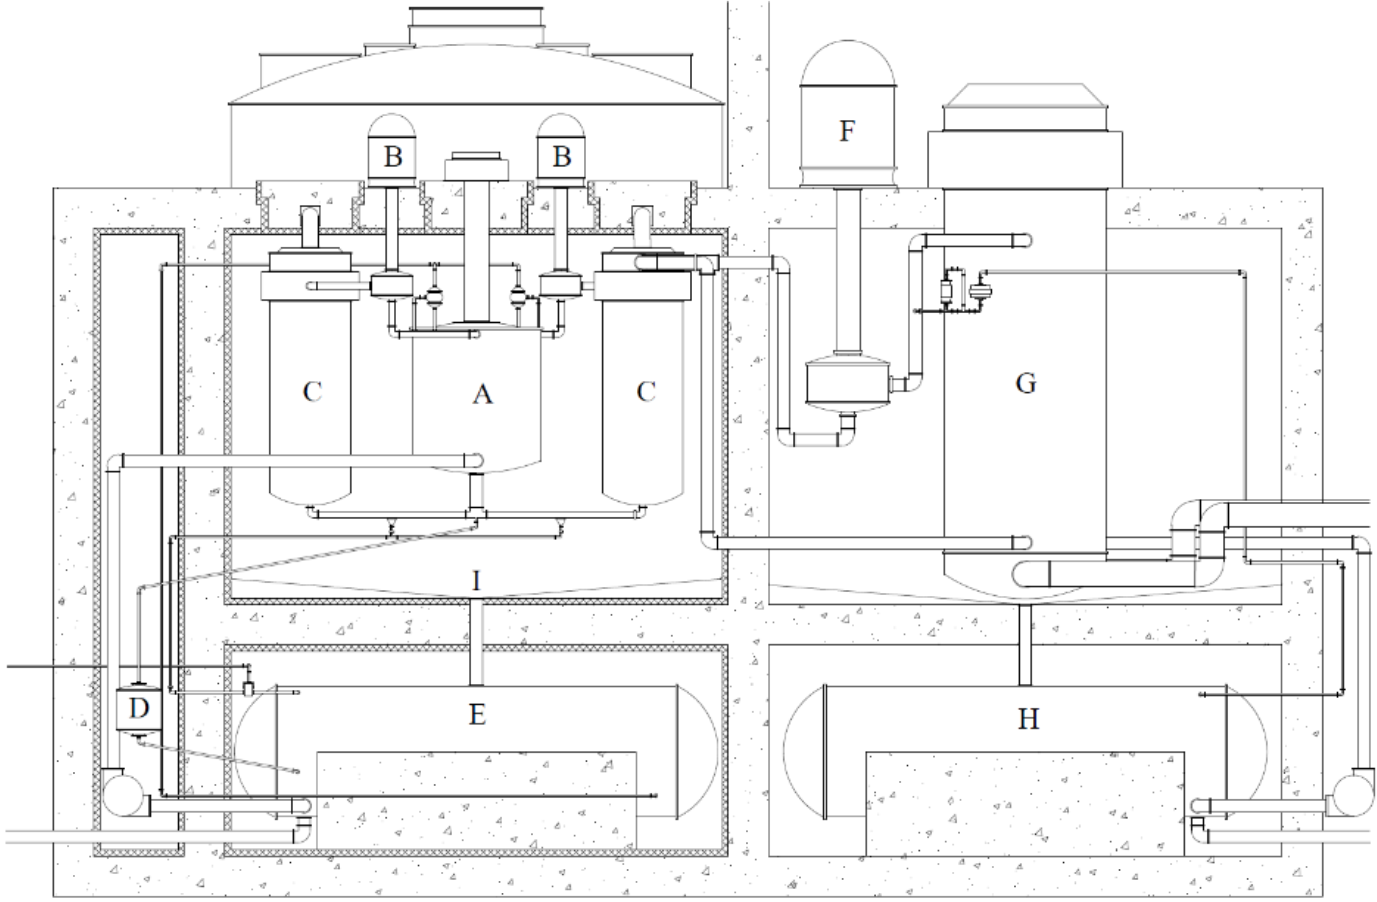
\includegraphics[width=\textwidth]{ch4/tap_simplified_scheme.png}
	\caption{Simplified schematic of the \gls{TAP} \gls{MSR} primary and  
		secondary loops (reproduced from the Transatomic Power Technical White 
		Paper \cite{transatomic_power_corporation_technical_2016}). Figure 
		legend: 
		A) reactor vessel, b) fuel salt pumps, C) primary heat exchangers, D) 
		freeze plug, E) primary loop drain tank, F) secondary loop salt pump, 
		G) 
		steam generator, H) secondary loop drain tank, I) fuel catch basin.}
	\label{fig:tap-primary-scheme}
\end{figure}

The \gls{TAP} design (figure~\ref{fig:tap-side-view}) is very similar to 
original \gls{MSRE} design developed by \gls{ORNL} 
\cite{haubenreich_experience_1970} but has two major innovations: 
the fuel salt composition and the moderator. The \gls{MSRE}'s 
LiF-BeF$_2$-ZrF$_4$-UF$_4$ salt has been substituted with LiF-UF$_4$ salt 
which allows for an increase in the uranium concentration within the fuel salt 
from 0.9 to 27.5\% while maintaining a relatively low melting point 
(490$^{\circ}$C compared with 434$^{\circ}$C for the original \gls{MSRE}'s 
salt) \cite{betzler_two-dimensional_2017}. The graphite has a very high 
thermal scattering cross section which makes it a perfect moderator but has 
a few major drawbacks: 
\begin{enumerate}[label=(\alph*)]
	\item low lethargy gain per collision requires a large volume of 
	moderator to be present to reach criticality, which leads to a larger core 
	and obstructs the core power density;
	\item even special reactor-grade graphite has relatively high porosity, 
	consequently, it holds gaseous \glspl{FP} (e.g., tritium, xenon) in pores;
	\item reactor graphite lifespan in a commercial reactor is 
	approximately 10 years \cite{robertson_conceptual_1971}.
\end{enumerate}
As previously mentioned, to resolve these issues, the \gls{TAP} concept uses 
zirconium hydride instead of graphite, allowing for a more compact core and a 
significant increase in power density. These two innovative design choices, 
together with a configurable moderator (the moderator-to-fuel ratio can be 
changed during operation), facilitate the deployment of this conceptual design 
in the current commercially available 5\% enriched \gls{LEU} fuel cycle. 
\begin{figure}[h] % replace 't' with 'b' to 
	\hspace{+2.2in}
	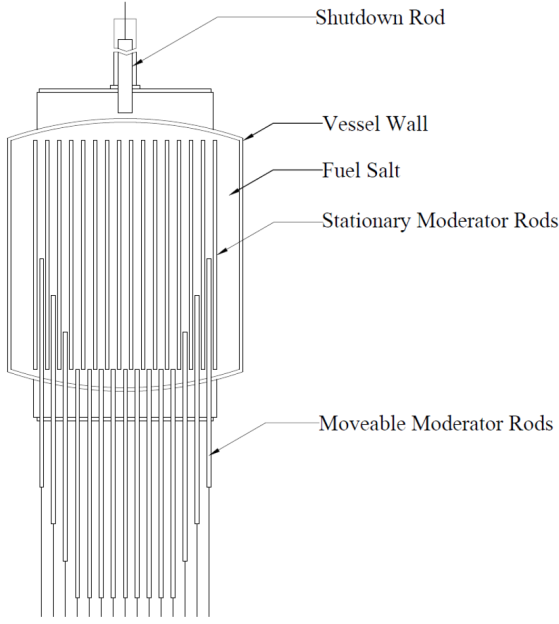
\includegraphics[width=0.65\textwidth]{ch4/tap_front_view.png}
	\caption{The \gls{TAP} \gls{MSR} schematic view showing movable moderator 
		rod bundles and shutdown rod (reproduced from Transatomic Power 
		White Paper \cite{transatomic_power_corporation_technical_2016}).}
	\label{fig:tap-side-view}
\end{figure}

The \gls{TAP} \gls{MSR} primary loop contains the reactor core volume  
(including the zirconium hydride moderator rods with silicon carbide  
cladding), pumps, and primary heat exchangers. Pumps circulate the  
LiF-(Act)F$_4$ fuel salt through the primary loop. The pumps, vessels, tanks, 
and piping are made of a nickel-based alloy (similar to Hastelloy-N\footnote{ 
Hastelloy-N is very common in \gls{MSR} concepts now, but was developed at 
\gls{ORNL} in the \gls{MSRE} program that started in the 1950s.}), which 
is highly resistant to corrosion in various molten salt environments. Inside 
the reactor vessel, near the zirconium hydride moderator rods, the fuel salt 
is in a critical configuration and generates heat. Table~\ref{tab:tap_tab} 
contains details of the \gls{TAP} system design which are taken from technical 
white paper \cite{transatomic_power_corporation_technical_2016} and a 
neutronics overview \cite{transatomic_power_corporation_neutronics_2016} as 
well as \gls{ORNL} analysis of the \gls{TAP} design 
\cite{betzler_two-dimensional_2017, betzler_assessment_2017-1}. 
%%%%%%%%%%%%%%%%%%%%%%%%%%%%%%%%%%%%%%%%
\begin{table}[h!]
	\caption{Summary of principal data for the \gls{TAP} \gls{MSR} 
		(reproduced from \cite{betzler_assessment_2017-1, 
		transatomic_power_corporation_technical_2016}). }
	\begin{tabularx}{\textwidth}{ s  s}
		\hline
		Thermal power   		& 1250 MW$_{th}  $       		\\ 
		Electric power		    & 520 MW$_e  $ 			 		\\ 
		Gross thermal efficiency& 44\%     				 		\\  
		Outlet temperature      & 620$^{\circ}$C         		\\ 
		Fuel salt components    & LiF-UF$_4$				    \\  
		Fuel salt composition   & 72.5-27.5 mole\%				\\  
		Uranium enrichment      & 5\% $^{235}$U          	    \\
		Moderator               & Zirconium Hydride (ZrH$_{1.66}$) rods \\
								& (with silicon carbide cladding)       \\
		Neutron spectrum        & intermediate at the \gls{BOL}             \\
		                        & thermal at the \gls{EOL}			\\
		\hline
	\end{tabularx}
	\label{tab:tap_tab}
\end{table}
%%%%%%%%%%%%%%%%%%%%%%%%%%%%%%%%%%%%%%%%%%%%%%%%%%%%%%%%%%%%%%%%%%%%%%%%%%%%%%%

\subsection{TAP core design}
In the \gls{TAP} core (Figure~\ref{fig:tap-core-ben}), fuel salt flows around 
moderator assemblies consisting of lattices of zirconium hydride rods clad in 
a corrosion-resistant silicone carbide. The \gls{TAP} reactor pressure vessel 
is a cylinder with an inner radius 150 cm, height 350 cm, and wall thickness 5 
cm made of a nickel-based alloy. 
\begin{figure}[t] % replace 't' with 'b' to 
	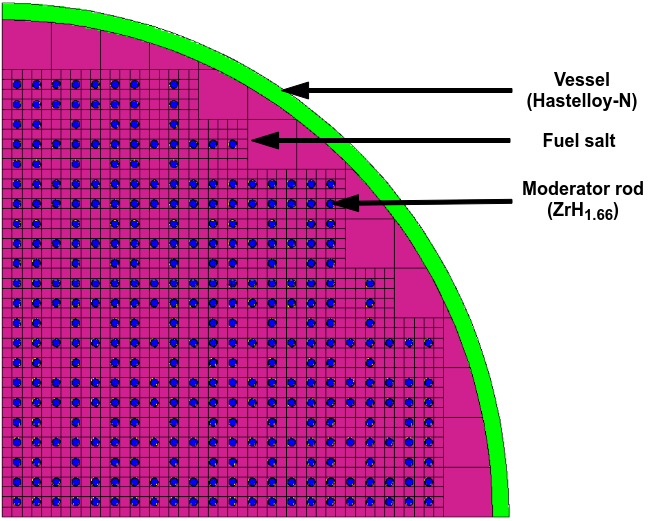
\includegraphics[width=\textwidth]{ch4/tap_core_ornl.png}
	\vspace{-0.35in}
	\caption{The \gls{TAP} \gls{MSR} schematic core view showing moderator 
		rods (reproduced from ORNL/TM-2017/475  
		\cite{betzler_assessment_2017-1}).}
	\label{fig:tap-core-ben}
\end{figure}

The \gls{SVF} in the core is parameter similar to wide-used moderator-to-fuel 
ratio and can be defined as:
\begin{align}
SVF &= \frac{V_F}{V_F+V_M} = \frac{1}{1+V_M/V_F}
\intertext{where}
V_F &= \mbox{the fuel volume $[m^3]$} \nonumber \\
V_M &= \mbox{the moderator volume $[m^3]$} \nonumber \\
V_M/V_F &= \mbox{the moderator-to-fuel salt ratio $[-]$.} \nonumber
\end{align}

Figure~\ref{fig:svf-predetermined} shows the \gls{SVF} variation during  
operation that shifts the reactor neutron energy spectrum from intermediate to 
thermal to maximize fuel burnup. At the \gls{BOL}, a high \gls{SVF} is 
selected to obtain relatively hard spectrum and enhance fertile material 
($^{238}$U) conversion into the fissile material ($^{239}$Pu) while the 
startup fissile material ($^{235}$U) inventory is still large. As fissile 
concentration in the fuel salt declines, an additional moderator are 
introduced to maintain criticality, leading to salt volume fraction decrease 
(see Figure~\ref{fig:svf-predetermined}).

Initial \gls{TAP} concept suggested vary salt volume fraction by inserting 
fixed-sized moderator rods via the bottom of the reactor vessel (for safety 
considerations), similarly to moving the control rods in a \gls{BWR}, as shown 
in Figure~\ref{fig:tap-side-view} 
\cite{transatomic_power_corporation_neutronics_2016}. The later \gls{TAP} 
concept proposes reducing the \gls{SVF} by reconfiguring the moderator rods 
during regular shutdown for reactor maintenance 
\cite{betzler_assessment_2017-1}. For the 
\gls{TAP} reactor, \gls{EOL} occurs when the maximum number of moderator rods 
are inserted into the core, and a further injection of fresh fuel salt does 
not alter criticality. Unmoderated salt is flowing in the annulus between the 
core, and the vessel wall provides for a potential reduction in fast neutron 
flux at the vessel structural material .
\begin{figure}[t] % replace 't' with 'b' to 
	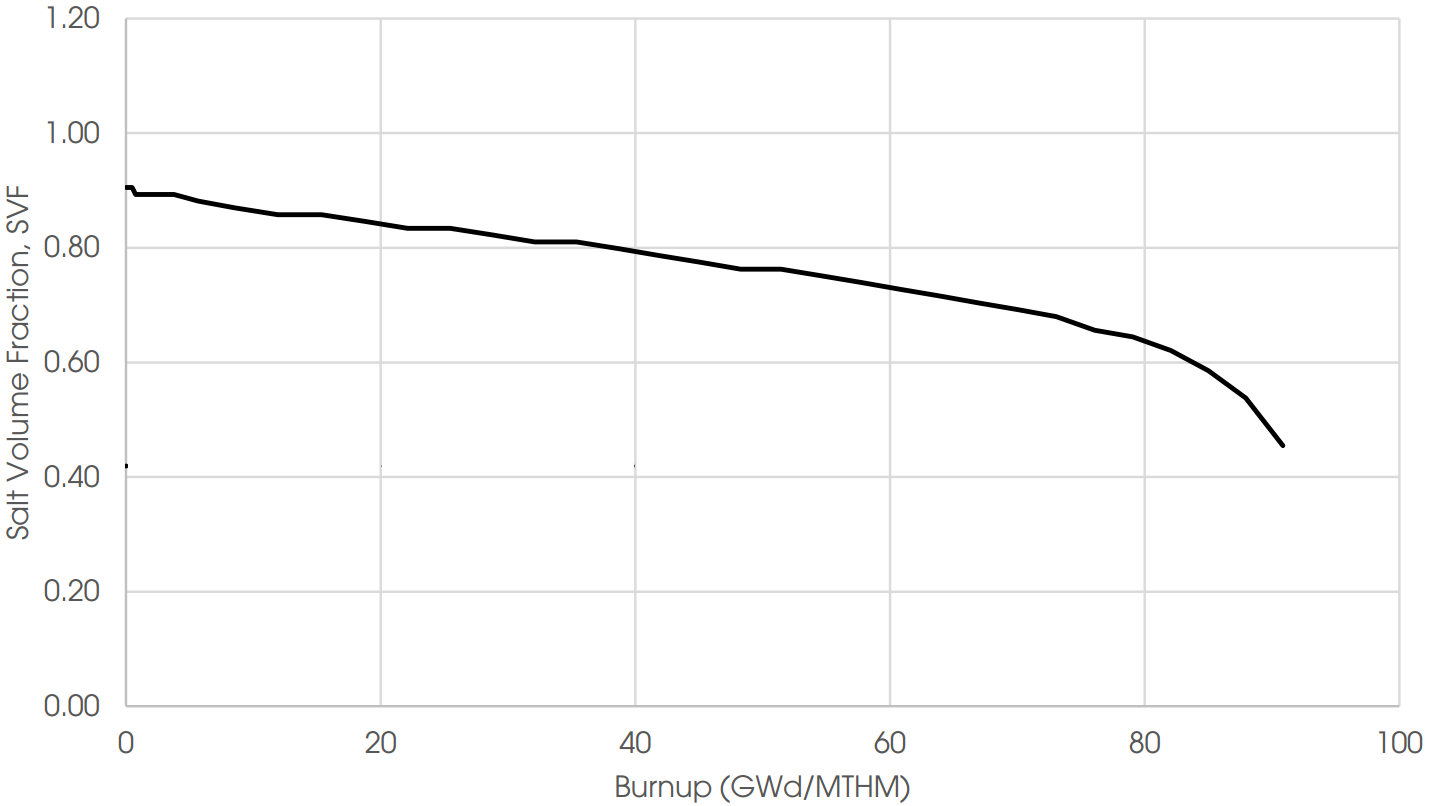
\includegraphics[width=\textwidth]{ch4/svf_predetermined.png}
	\caption{The change in SVF as a function of burnup in the \gls{TAP} 
	reactor (reproduced from Transatomic Power Neutronics Overview  
	\cite{transatomic_power_corporation_neutronics_2016}).}
	\label{fig:svf-predetermined}
\end{figure}


\subsection{Serpent 2 full-core model} \label{sec:tap_model}
Nest and lattice geometry types as well as universe transformation 
capabilities of Serpent \cite{leppanen_serpent_2014}  are employed to 
represent \gls{TAP} core. Figure~\ref{fig:tap-serpent-plan} shows the $XY$ 
section of whole-core configuration at the expected reactor operational level 
when all control rods are fully withdrawn. Figures~\ref{fig:tap-serpent-elev} 
and ~\ref{fig:tap-serpent-elev-zoom} show a longitudinal section of the 
reactor. This model contains the moderator rods with silicon carbide cladding, 
pressure vessel, and inlet and outlet plena (Table~\ref{tab:tap_model_param}). 
Fuel salt flows around rectangular moderator assemblies consisting of lattices 
of small-diameter zirconium hydride rods in a corrosion-resistant material. 
The salt volume fraction for Figure ~\ref{fig:tap-serpent-plan} is 0.917204, 
which means the modeled core is under-moderated and has intermediate neutron 
spectrum. Quarter-core configurations of the \gls{TAP} core with various salt 
volume fraction, used in the current work to maintain criticality for 
reasonable operational period ($>20$ years), are listed in 
Table~\ref{tab:tap_adjustable_core},Figures~\ref{fig:tap-406-681}, and 
\ref{fig:tap-840-1668} in Appendix~\ref{appex:geometries}.
\begin{figure}[htp!] % replace 't' with 'b' to 
	\centering
	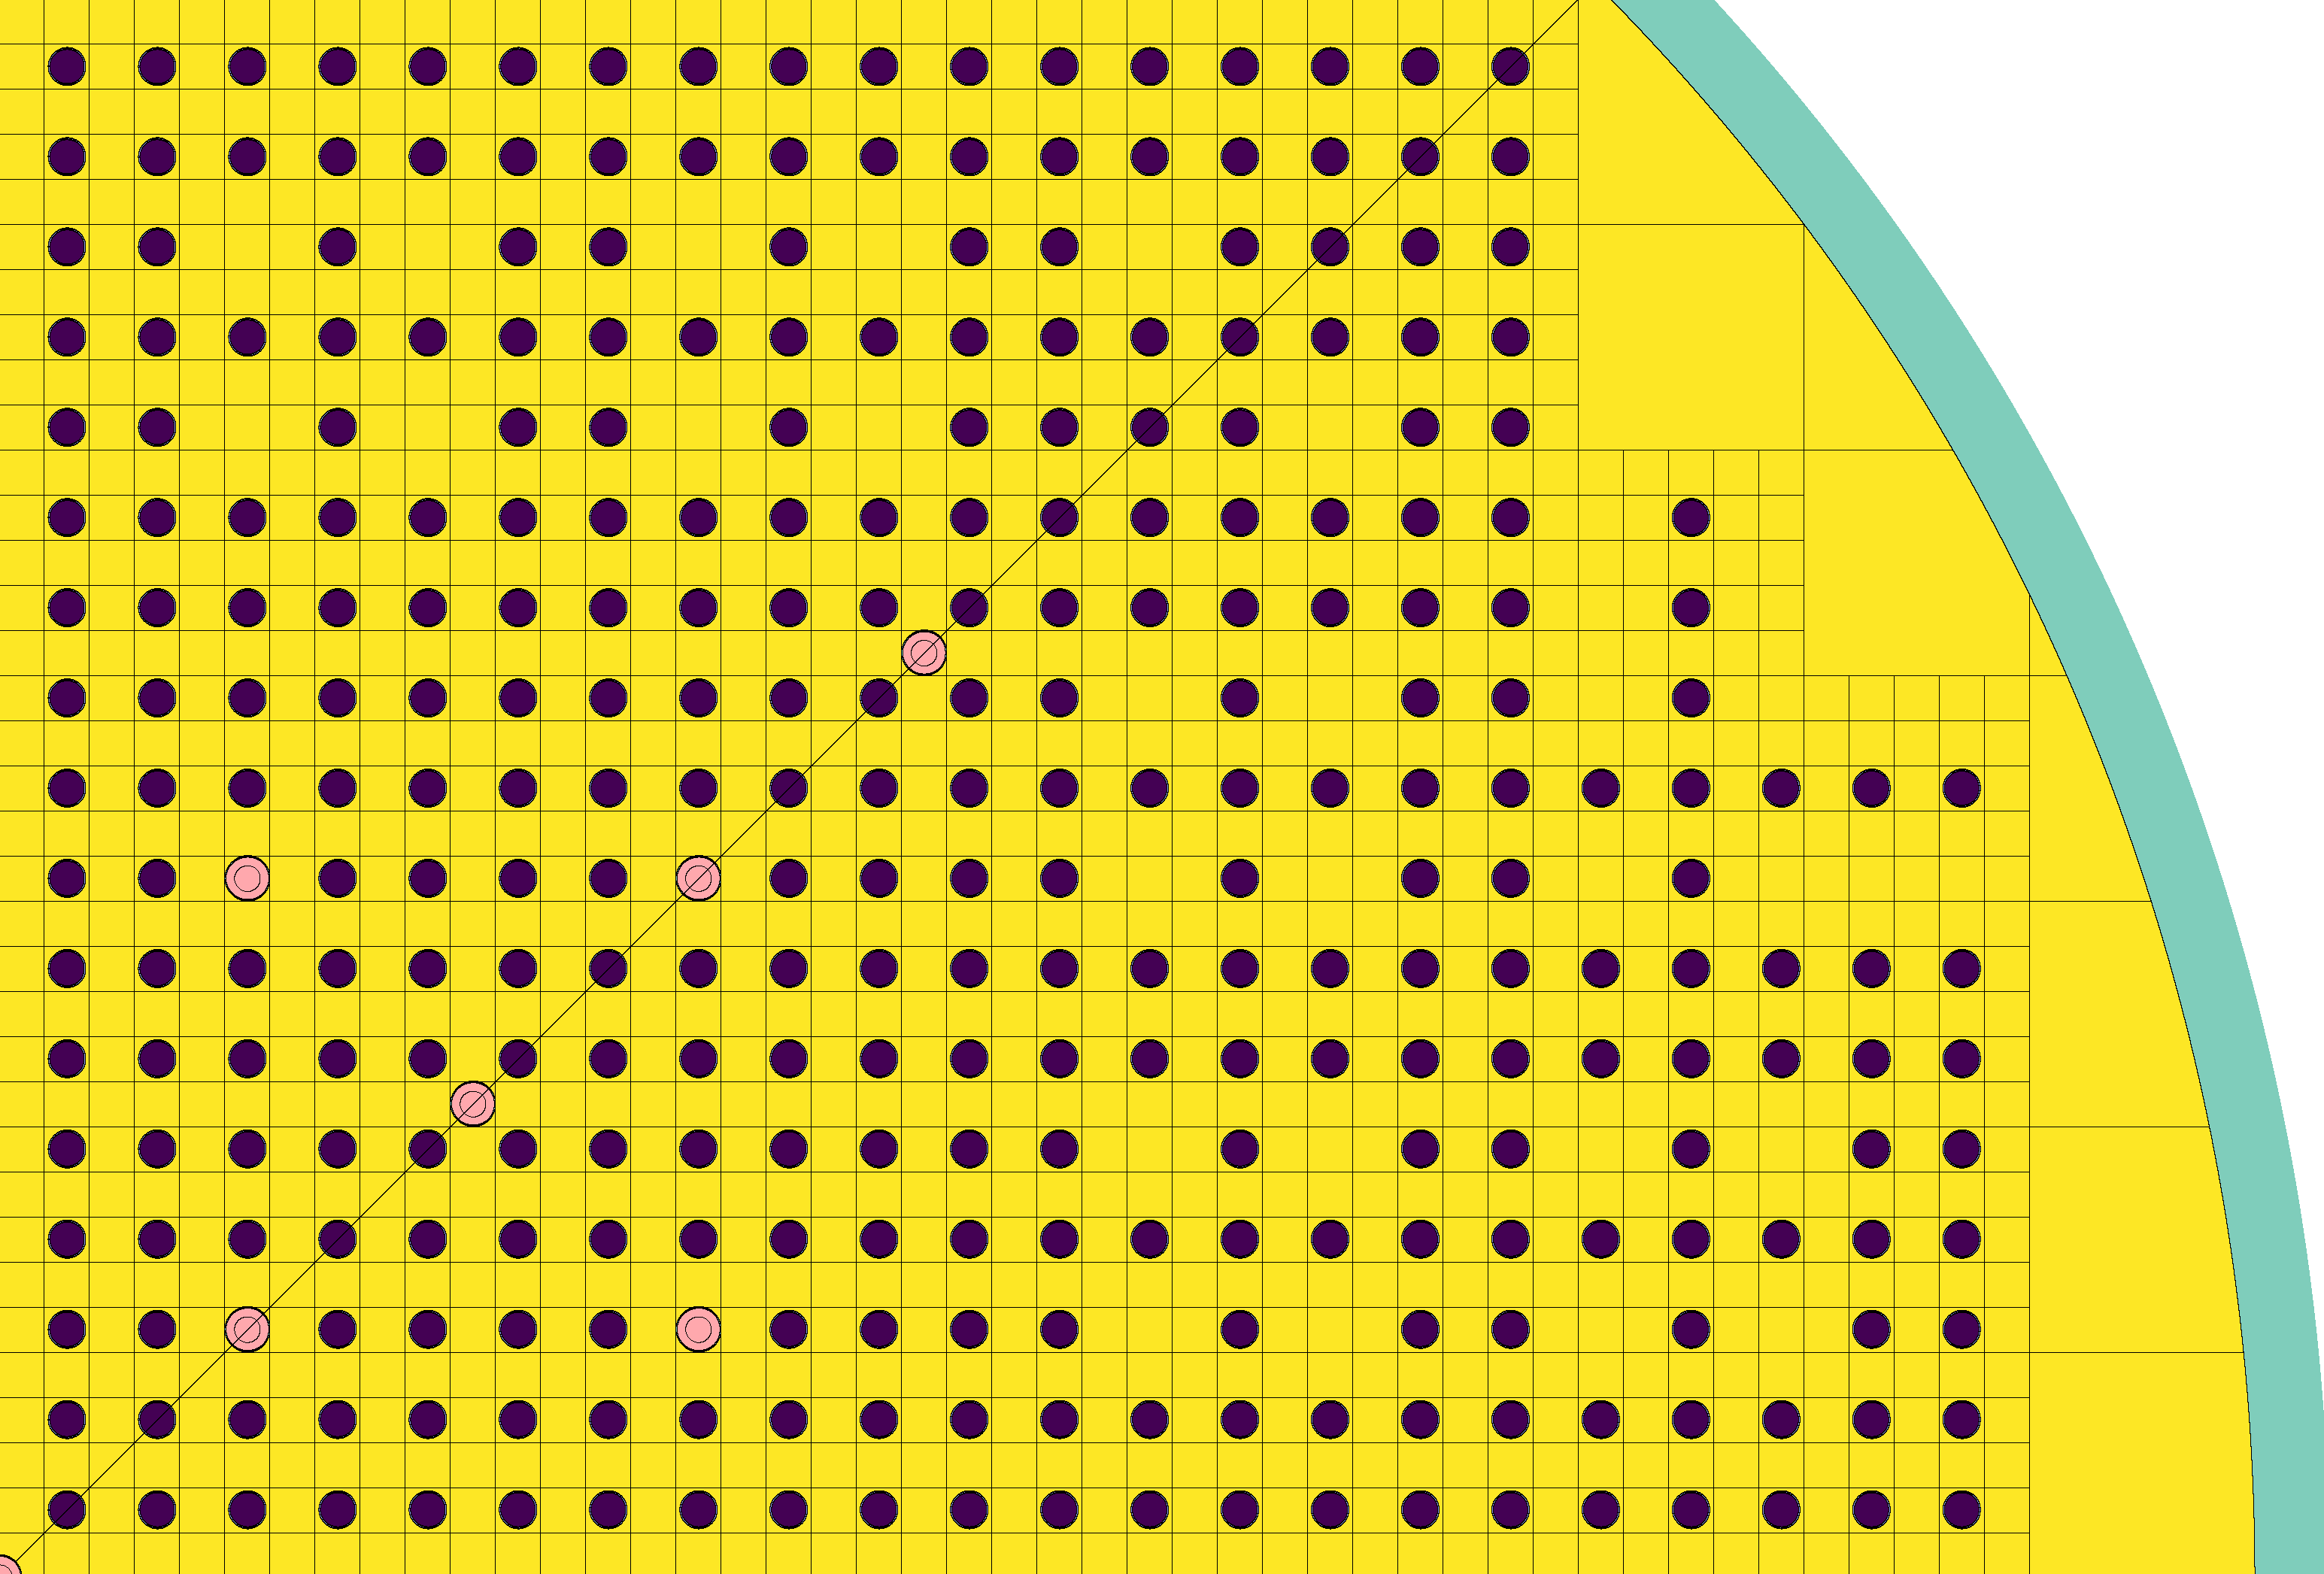
\includegraphics[width=0.75\textwidth]{ch4/tap_plan_view_serpent_347.png}
	\caption{An $XY$ section of the \gls{TAP} model at horizontal midplane 
		with fully withdrawn control rods at \gls{BOL} (347 moderator rods, 
		salt volume fraction is equal 0.917204). 
		The violet color represents zirconium hydride, and the yellow 
		represents fuel salt. 
		The blue color shows Hastelloy-N, a material used for the vessel wall, 
		and the pink color is the air.}
	\label{fig:tap-serpent-plan}
\end{figure}

\begin{figure}[htp!] % replace 't' with 'b' to 
	\centering
	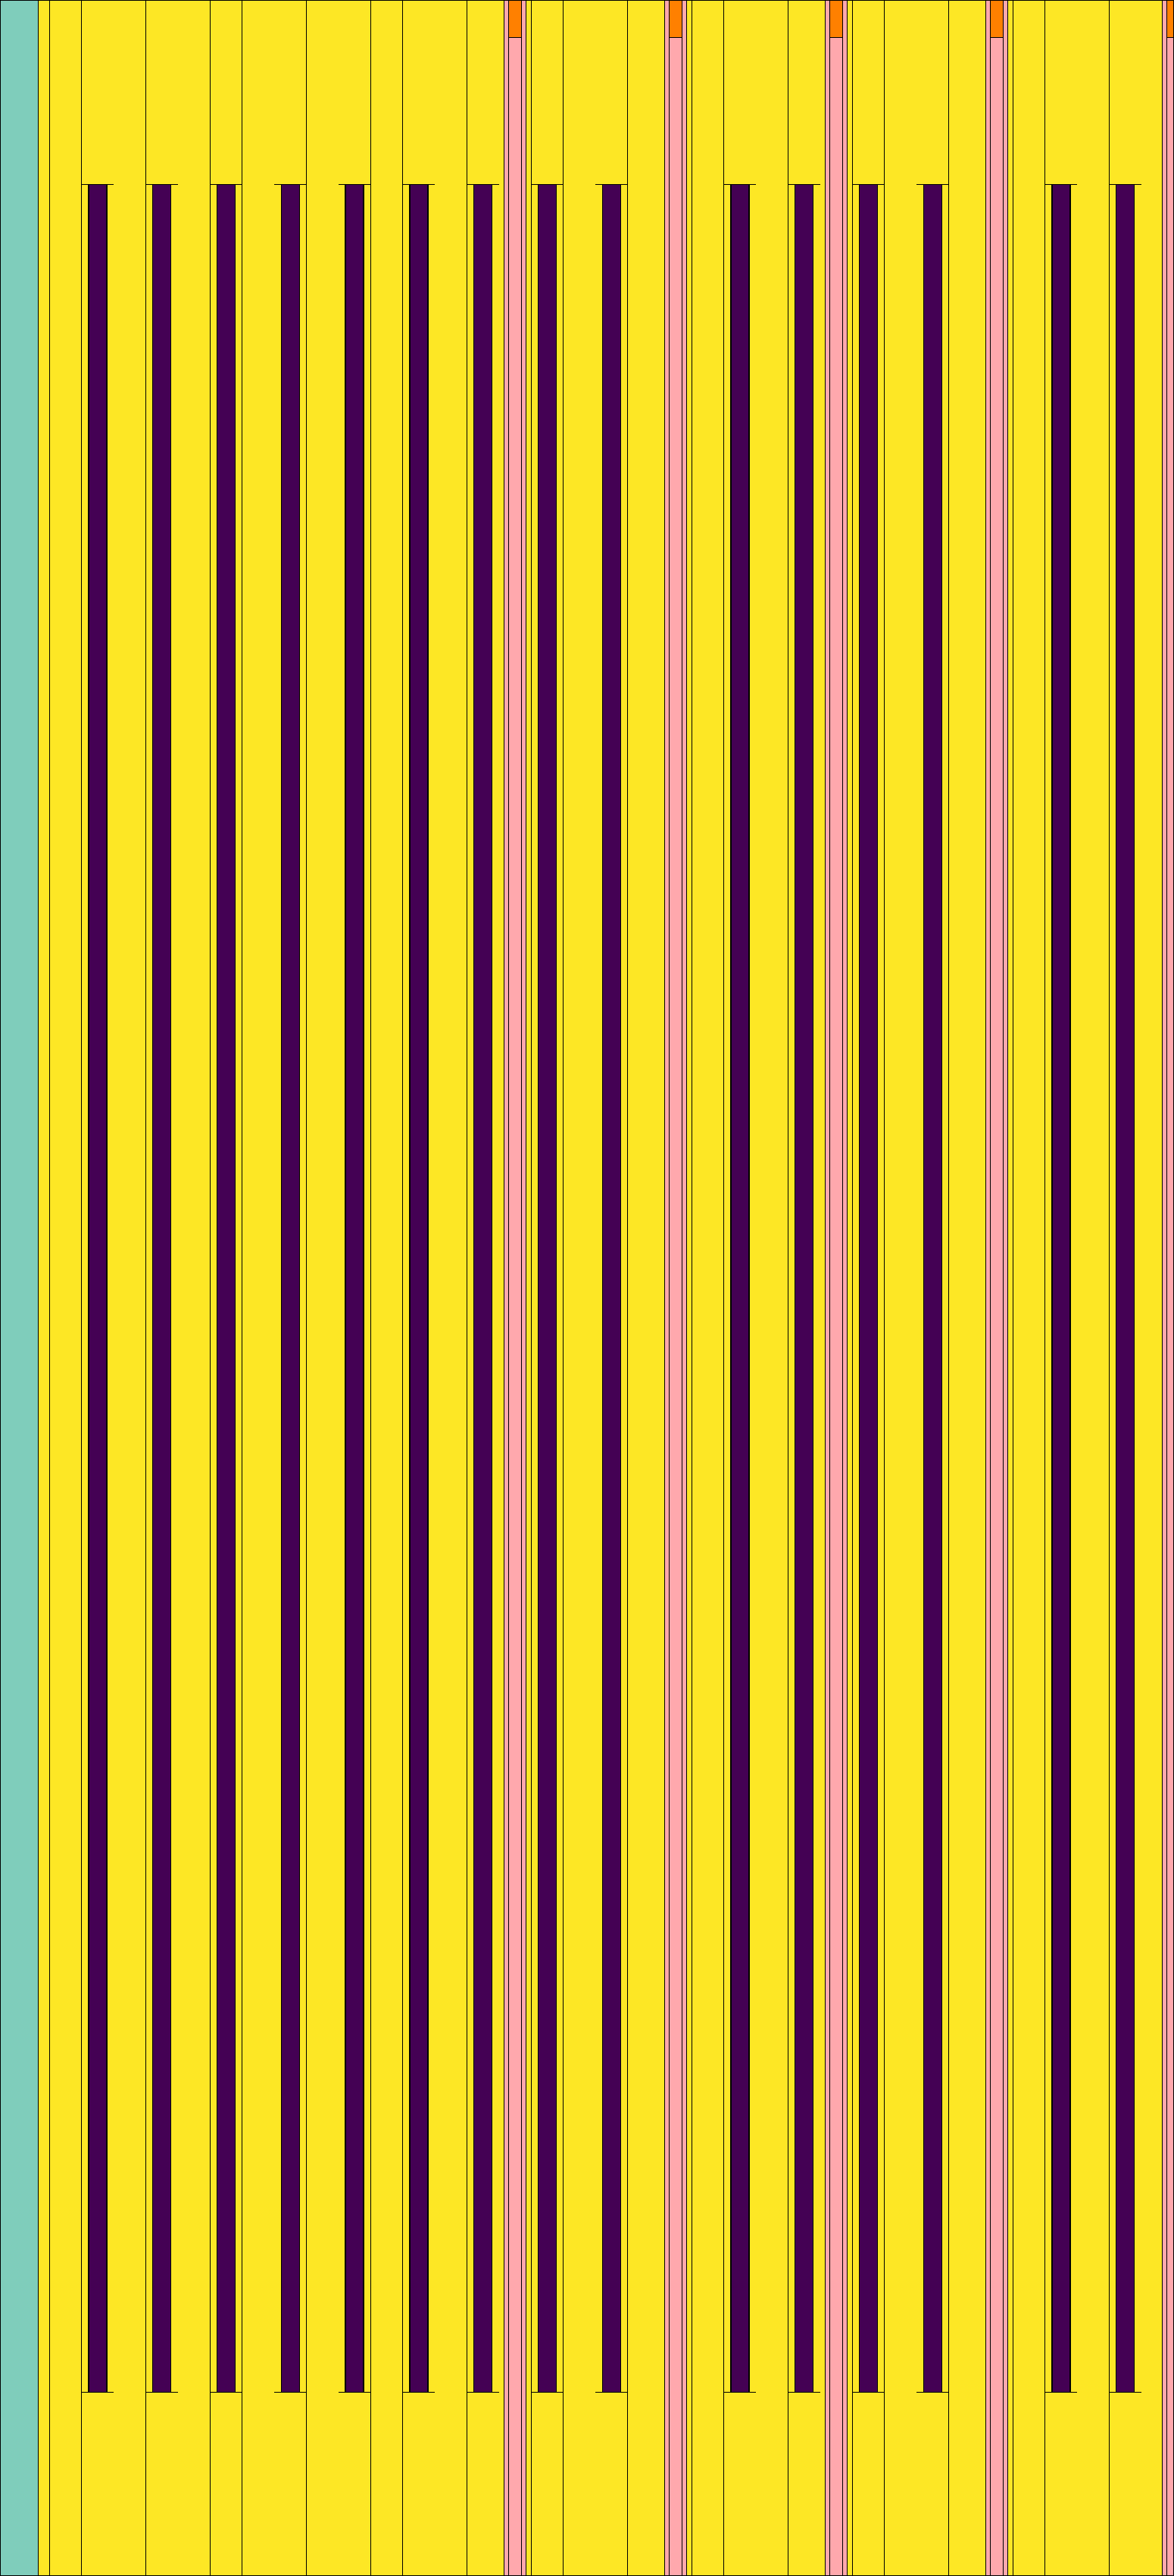
\includegraphics[width=0.6\textwidth]{ch4/tap_elev_view_serpent_347.png}
	\caption{45$^{\circ}$ $XZ$ section of the \gls{TAP} core model.}
	\label{fig:tap-serpent-elev}
\end{figure}

To represent the reactivity control system, the model has: 
\begin{enumerate}[label=(\alph*)]
	\item control rod guide tubes made of nickel-based alloy;
	\item control rods represented as a Boron Carbide (B$_4$C) cylinders 
	with a thin Hastelloy-N coating;
	\item air inside guide tubes and control rods;
\end{enumerate}
The control rods must be able to suppress excess reactivity at the \gls{BOL} 
when the core configuration is the most reactive and the neutron spectrum is 
the hardest. The control rod design shown on 
Figures~\ref{fig:tap-serpent-plan} and \ref{fig:tap-serpent-elev-zoom} is 
comprised of a cluster of 25 rods that provide a total reactivity worth of 
$4226\pm9pcm$ at the \gls{BOL}.

\begin{figure}[htp!] % replace 't' with 'b' to 
	\centering
	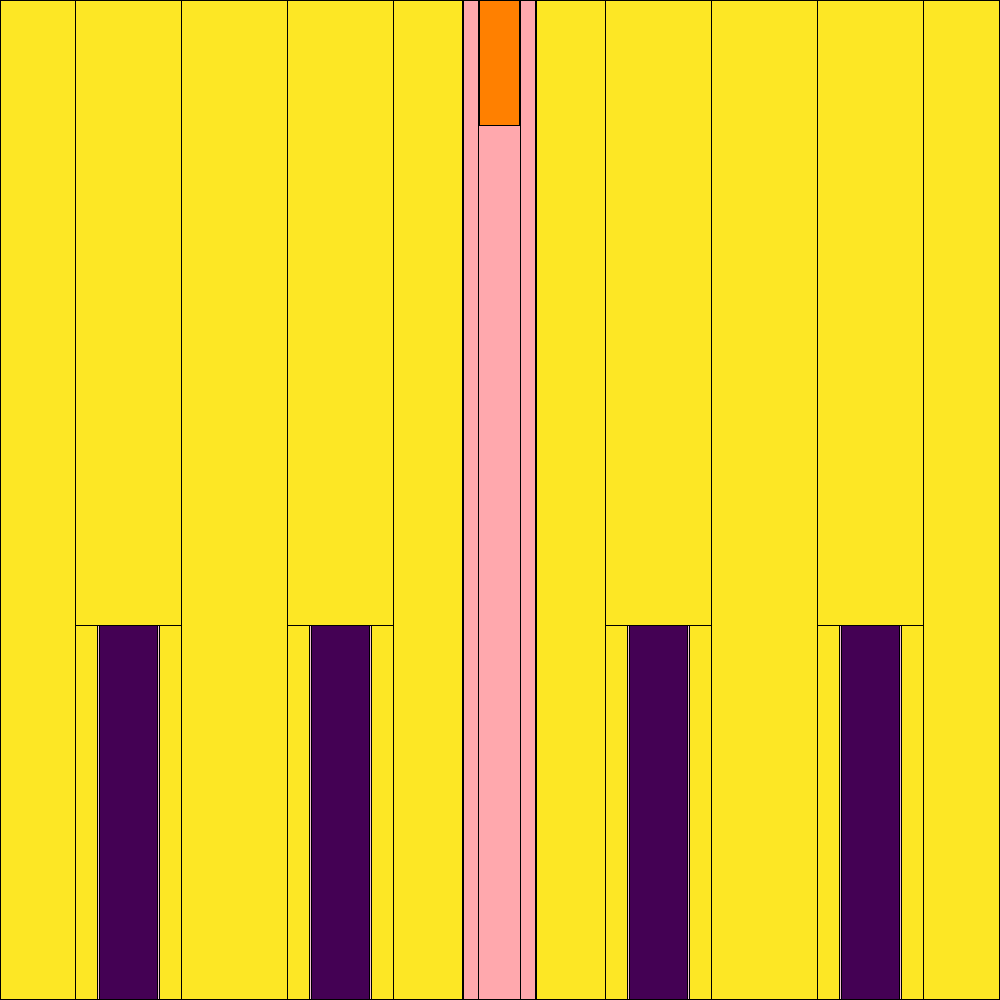
\includegraphics[width=0.55\textwidth]{ch4/tap_elev_view_zoomed_serpent.png}
	\caption{Zoomed $XZ$ section of the top of the moderator and control rods  
		in the \gls{TAP} model. The orange color shows Boron Carbide 
		(B$_4$C) absorbers used for control rods.}
	\label{fig:tap-serpent-elev-zoom}
\end{figure}
%%%%%%%%%%%%%%%%%%%%%%%%%%%%%%%%%%%%%%%%%%%%%%%%%%
\begin{table}[ht!]
	\caption{Geometric parameters for the full-core 3D model of the 
		\gls{TAP} (reproduced from Betzler \emph{et al.} 
		\cite{betzler_assessment_2017-1}). }
	\centering
	\begin{tabularx}{0.9\textwidth}{s s x p{0.14\textwidth}}
		\hline
		\textbf{Component}&\textbf{Parameter}&\textbf{Value}& \textbf{Unit}   
		\\ \hline
		\multirow{4}{*}{\begin{tabular}[c]{@{}l@{}}Moderator\\ 
				rod\end{tabular}} 
		& Cladding thickness      	  			    & 0.10 & cm				 
		\\  
		& Radius 				      	  			& 1.15 & cm				 
		\\  
		& Length				      	  			& 3.0  & m				 
		\\  
		& Pitch				      	  			& 3.0  & cm  			 \\ 
		\hline 
		
		\multirow{2}{*}{\begin{tabular}[c]{@{}l@{}}Moderator\\ 
				assembly\end{tabular}} 
		& Array				      	  			& 5 $\times$ 5 & 
		rods$\times$rods \\  
		& Pitch				      	  			& 15.0 & cm    				 
		\\  \hline
		
		\multirow{4}{*}{\begin{tabular}[c]{@{}l@{}}Core\end{tabular}}          
		& Assemblies  				   	  			& 268  & assemblies/core 
		\\  
		& Inner radius			      	  			& 1.5  & 
		m    				 \\  
		& Plenum height			   	  			& 25.0 & cm    				 
		\\  
		& Vessel wall thickness     	  			& 5.0 & 
		cm    				 \\ \hline            
	\end{tabularx}
	\label{tab:tap_model_param}
\end{table}
%%%%%%%%%%%%%%%%%%%%%%%%%%%%%%%%%%%%%%%%%%%%%%%%

The control rod cluster is modeled using the \textbf{TRANS} Serpent 2 feature, 
which allows the user to easily change the control rod position during the 
simulation. The current works assumed that all control rods are fully 
withdrawn from the core (Figure~\ref{fig:tap-serpent-elev-zoom}), but user can 
use SaltProc v1.0 reactivity control capabilities to change control 
rod position during operation. In this dissertation, all figures of the core 
were generated using the built-in Serpent plotter.


\subsection{TAP fuel salt reprocessing system}
The \gls{TAP} nuclear island contains a fission product removal system. 
Gaseous \glspl{FP} are continuously removed using an off-gas system while 
liquid and 
solid \glspl{FP} are extracted via a chemical processing system. As these 
byproducts are gradually removed, a small quantity of fresh fuel salt is 
regularly added to the primary loop. This process conserves a constant fuel 
salt mass and keeps the reactor critical. In contrast with the \gls{MSBR} 
reprocessing system, the \gls{TAP} design does not need a protactinium 
separation and isolation system because it operates in a uranium-based 
single-stage fuel cycle. The authors of the \gls{TAP} concept suggested three 
distinct fission product removal methods 
\cite{transatomic_power_corporation_neutronics_2016}:
\paragraph{Off-Gas System:} The off-gas system removes gaseous fission 
products such as krypton and xenon, which are then compressed and stored 
temporarily until they have decayed to the background radiation level. Trace 
amounts of tritium are also removed and bottled in a liquid form via the same 
process. Also, the off-gas system directly removes a small fraction of the 
noble metals.
\paragraph{Metal Plate-Out/Filtration:} A nickel mesh filter removes noble and 
semi-noble metal solid fission products as they plate out onto internal surface
of the filter.
\paragraph{Liquid Metal Extraction:} Lanthanides and other non-noble metals 
stay dissolved in the fuel salt. They generally have a lower capture cross 
section and thus absorb fewer neutrons than $^{135}$Xe, but their extraction 
is essential to ensure normal operation. In the \gls{TAP} reactor, lanthanide 
removal is accomplished via a liquid-metal/molten salt extraction process 
similar to that developed for \gls{MSBR} by \gls{ORNL}  
\cite{robertson_conceptual_1971}. The process converts the dissolved 
lanthanides into a well-understood oxide waste form, similar to that of 
\gls{LWR} \gls{SNF}. This oxide waste comes out of the \gls{TAP} reprocessing 
plant in ceramic granules and can be sintered into another convenient form for 
storage \cite{transatomic_power_corporation_technical_2016}.

Figure~\ref{fig:tap-reproc} shows the principal design of the \gls{TAP} 
primary loop, including an off-gas system, nickel mesh filter, and lanthanide 
chemical extraction facility. Similarly to the \gls{MSBR}, an off-gas system 
is also based on a simple process of helium sparging through fuel salt with 
consequent gas bubbles removed before returning the fuel salt to the core. 
Nevertheless, one crucial difference must be noted: the \gls{MSBR} gas 
separation system suggested helium injection and subsequent transport of the 
voids throughout the primary loop, including the core for at least ten full 
loops \cite{robertson_conceptual_1971}. It is a significant concern for safe, 
stable operation because the increase of void fraction in the fuel salt when 
it enters back to the core would cause unpredictable reactivity change. This 
drawback can be overcome by using an effective gas separator for stripping 
helium/xenon bubbles before returning the salt to a primary loop 
(Figure~\ref{fig:tap-reproc}, blue block). 
\begin{figure}[htp!] % replace 't' with 'b' to 
	\centering
	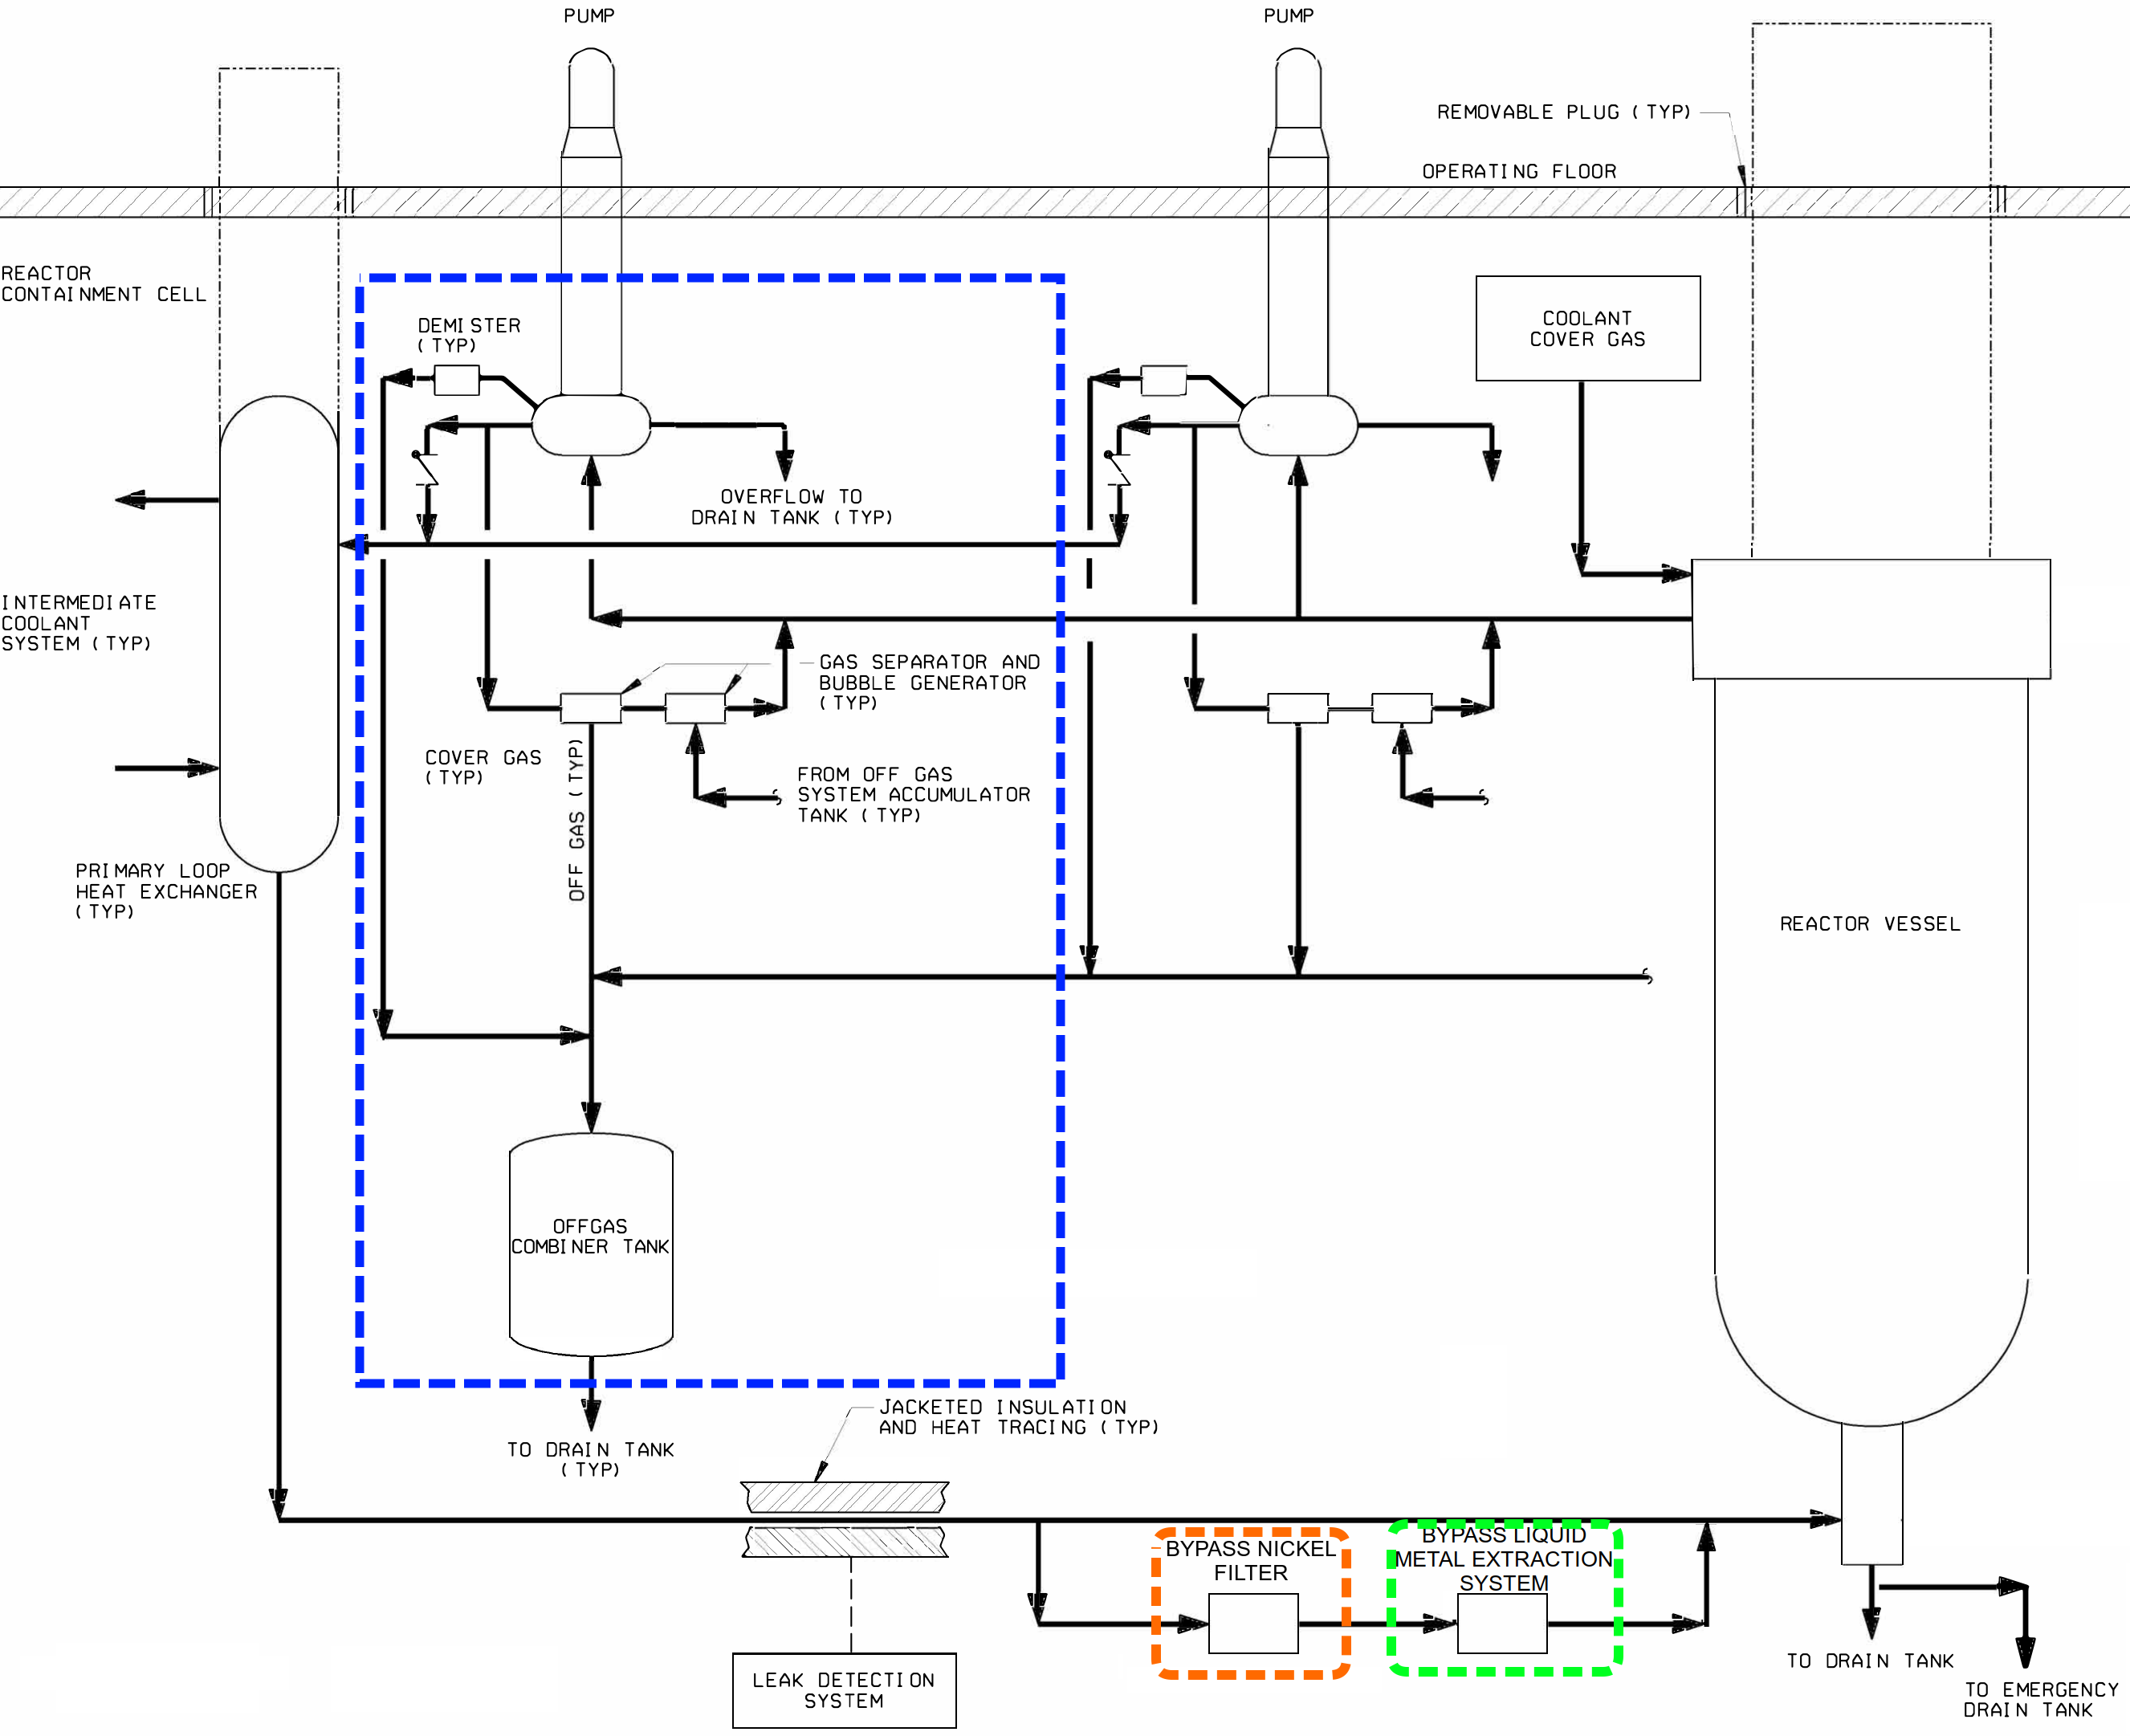
\includegraphics[width=\textwidth]{ch4/tap_primary_loop.png}
	\caption{Simplified \gls{TAP} primary loop design including off-gas system 
		(blue), 
		nickel filter (orange) and liquid metal extraction system (green) 
		(reproduced from \cite{transatomic_power_transatomic_2019}).}
	\label{fig:tap-reproc}
\end{figure}

Noble and semi-noble metal solid fission products tend to plate out onto metal 
surfaces including piping, heat exchanger tubes, reactor vessel inner surface, 
etc. Previous research by \gls{ORNL} \cite{robertson_conceptual_1971} reported 
that about 50\% of noble and semi-noble metals would plate out inside 
\gls{MSBR} systems without any special treatment. To improve the extraction 
efficiency of these fission products, the \gls{TAP} concept suggested 
employing a nickel mesh filter located in a bypass stream in the primary loop 
(Figure~\ref{fig:tap-reproc}, orange block). The main idea of this filter is 
to create a maze with large metal (nickel) surface area. The fuel salt is  
flowing throughout the filter and noble metals plate-out on the internal  
filter surface. 

This Liquid Metal Extraction process for the \gls{TAP} concept has been 
adopted from the \gls{MSBR}. The \gls{MSRE} demonstrated a liquid-liquid 
extraction process for removing rare earths and lanthanides from fuel salt and 
estimated efficiency of this process. Removal efficiency ($\epsilon_{RE}$) of  
this process is the function of salt mass flow rate, liquid bismuth mass 
flow rate, interfacial areas between salt and metal, and mass transfer 
coefficient for each noble metal species. The most recent research for LiF 
salt (for the \gls{MSFR} concept) reported the following form of extraction 
efficiency correlation \cite{rodrigues_actinide/lanthanide_2015}:
\begin{align} 
\epsilon_{RE} &= \frac{1}{1+10^{\lambda}} \nonumber \\
&= \frac{1}{1+10^{f(A, \dot{m}_{Bi}, \dot{m}_{salt}, N, K)}} \label{eq:re_eff}
\intertext{where}
A&= \mbox{metal-to-salt interface area} \nonumber \\
\dot{m}_{Bi}&= \mbox{bismuth mass flow rate} \nonumber \\
\dot{m}_{salt}&= \mbox{salt mass flow rate} \nonumber \\
N&= \mbox{number of stages} \nonumber \\
K&= \mbox{liquid phase mass transfer coefficient} \nonumber 
\end{align}
Correlations are different for various lanthanides and can be determined from 
experimental data and/or existing analytical models 
\cite{mcneese_engineering_1971, delpech_possible_2012, 
	rodrigues_actinide/lanthanide_2015}.

In fact, due to similarities in reprocessing schemes, the \gls{TAP} project 
reported almost the same set of elements for removal and similar effective 
cycle times as suggested for \gls{MSBR} (Table~\ref{tab:reprocessing_list}). 
The \gls{TAP} neutronics whitepaper specifies additional low-probability 
fission products and gases that should be removed during operation. These 
elements are categorized into the previously defined processing groups, but 
the removal rates of most of these elements (i.e., all except for hydrogen) 
are very low.

Details of gas removal and fuel reprocessing systems have historically 
been conceptual. Accordingly, liquid-fueled system designs including the 
\gls{TAP} concept usually assume ideal (rather than realistically constrained) 
removal efficiencies for reactor performance simulations. For the proposed 
work, a realistic online reprocessing system and reactor model will be created 
to capture the dynamics of fuel composition evolution during reactor 
operation. Gas removal efficiency will be represented in that model as a 
variable, described using mathematical correlation from Chapter 2 (see  
Equation~\ref{eq:gas_eff}). For the other \glspl{FP}, a fixed\footnote{ 
	Published information about dynamics of extraction efficiency during 
	reactor 
	operation for seminoble metals, volatile fluorides, and rare earths is 
	insufficient to inform a variable removal efficiency.}, non-ideal 
extraction efficiency based on cycle time from 
Table~\ref{tab:reprocessing_list} will be used in the fuel reprocessing model.

%%%%%%%%%%%%%%%%%%%%%%%%%%%%%%%%%%%%%%%%
\begin{table}[htbp!]
	\centering
	\caption{The effective cycle times for fission products removal  from the 
		\gls{TAP} reactor (reproduced from \cite{betzler_implementation_2017} 
		and 
		\cite{transatomic_power_corporation_neutronics_2016}).}
	\begin{tabular}{p{0.2\textwidth} p{0.42\textwidth} p{0.12\textwidth} 
			p{0.16\textwidth}}
		\hline 
		%\begin{tabularx}{\linewidth}{l X} \toprule 
		\textbf{Processing group} & \qquad\qquad\qquad \textbf{Nuclides} & 
		\textbf{Removal Rate (s$^{-1}$)} & \textbf{Cycle time (at full power)} 
		\\ [5pt] \hline 
		\multicolumn{3}{c}{\textit{Elements removed in \gls{MSBR} concept and 
				adopted for the \gls{TAP}} \cite{robertson_conceptual_1971}} \\
		Volatile gases & Xe, Kr								  & 5.00E-2 & 20 
		sec \\ [5pt]
		Noble metals & Se, Nb, Mo, Tc, Ru, Rh, Pd, Ag, Sb, Te & 5.00E-2 & 20 
		sec \\ [5pt]
		Seminoble metals & Zr, Cd, In, Sn	  				  & 5.79E-8 & 200 
		days \\ [5pt]
		Volatile fluorides & Br, I 							  & 1.93E-7 & 60 
		days \\ [5pt]
		Rare earths & Y, La, Ce, Pr, Nd, Pm, Sm, Gd           & 2.31E-7 & 50 
		days \\ [5pt]
		\qquad & Eu & 2.32E-8 & 500 days \\ [5pt]
		Discard & Rb, Sr, Cs, Ba & 3.37E-9 & 3435 days \\ [5pt] 
		\hline
		
		\multicolumn{3}{c}{\textit{Additional elements removed} 
			\cite{transatomic_power_corporation_neutronics_2016, 
				betzler_implementation_2017}  } \\
		Volatile gases & H								  	& 5.00E-2 & 20 
		sec    \\ [5pt]
		Noble metals & Ti, V, Cr, Cu						& 3.37E-9 & 3435 
		days \\ [5pt]
		Seminoble metals & Mn, Fe, Co, Ni, Zn, Ga, Ge, As   & 3.37E-9 & 3435 
		days \\ [5pt]
		Rare earths & Sc									& 3.37E-9 & 3435 
		days \\ [5pt]
		Discard & Ca										& 3.37E-9 & 3435 
		days \\ [5pt] 
		\hline
	\end{tabular}
	\label{tab:reprocessing_list}
	\vspace{-0.9em}
\end{table}
%%%%%%%%%%%%%%%%%%%%%%%%%%%%%%%%%%%%%%%%%%%%%%%%%%%%%%%%%%%%%%%%%%%%%%%%%%%%%%%



\section{Long-term depletion case demonstration and validation}
\subsection{Fuel salt isotopic composition dynamics}

\section{Reactor load following analysis}

\section{Prototype design for the xenon removal system}

\section{Concluding remarks}
\chapter{Tool demonstration for load-following and safety analysis: 
Transatomic Power MSR}
\paragraph*{Short-term (transient).} I performed the 24-hour-long depletion 
simulation with changing, load following reactor power with the fine time 
resolution (variable depletion step from 1 to 30-min). The depletion 
calculation for the \gls{TAP} in load following regime capture the effects of 
xenon poisoning and evaluate the benefit of using an online gas removal system.

In this chapter, I also analyze the reactor load-following capability for 
various moderator configurations and fuel salt compositions to bound design 
parameters of gas removal system to ensure load-following operation. 
\section{Reactor load following analysis}

\section{Prototype design for the xenon removal system}

\section{Concluding remarks}
%\chapter{Tool demonstration for load-following and safety analysis: Molten 
Salt Breeder Reactor}
Previous chapter shown that the \gls{TAP} \gls{MSR} is unaffected by the xenon 
poisoning effect during power variation because it has relatively fast neutron 
energy spectrum. 
While long-term performance 
metrics such as fuel utilization would definitely benefit from online removal 
of poisonous fission products, the gas removal system is unessential to ensure 
the \gls{TAP} system operation during short-term transient with significant 
power drop and following restart. However, Chapter 5 clearly demonstrated the 
noble gas removal strong impact on the reactor neutronics during power 
adjustments. Thus, another liquid-fueled \gls{MSR} design with thermal 
spectrum (not epithermal like in the \gls{TAP} core) should be considered to 
investigate benefits of the online gas removal for load-following 
operation.	

This chapter presents fuel salt depletion analysis with SaltProc during a
short-term power transient to evaluate load-following capabilities of the 
graphite-moderated molten salt reactor design with a thermal neutron energy 
spectrum - \gls{MSBR}. The details of the \gls{MSBR} design, the full-core 
Serpent model, and 
results of long-term depletion simulation with SaltProc are described in 
Chapter 3. I simulate the load-following transient postulated in 
Section~\ref{sec:worst-load} using methodology described in Chapter 5. To 
investigate the effect of noble gas 
removal efficiency on load-following operation, I consider three various 
regimes of the gas removal system operation:
\begin{enumerate}[label=(\alph*), noitemsep, topsep=0pt]
	\item no gas removal ($\epsilon_{Xe}=0.0$);
	\item moderate gas removal efficiency ($\epsilon_{Xe}=0.536$);
	\item high gas removal efficiency ($\epsilon_{Xe}=0.915$).
\end{enumerate}
I then calculate a major safety and operational parameters for all three 
regimes at various moments of the transient to make sure that the critical 
safety margins are maintained. Finally, I compare the \gls{TAP} \gls{MSR} and 
\gls{MSBR} behavior during the postulated load-following transient.


\section{Depletion analysis results}
Using the methodology described previously in Chapter 5, the \gls{MSBR} 
full-core depletion analysis was performed using SaltProc v1.0. I 
used 30-minutes depletion time step to capture rapid changes in reactivity. 
The Equation~\ref{eq:time-xe-max} predicted the time after shutdown when 
$^{135}$Xe concentration peaks ($t^{max}_X$) in the range from 6.8h 
($\epsilon_{Xe}=0.0$, 30 years after startup) to 7.5h ($\epsilon_{Xe}=0.915$, 
\gls{BOL}). The $t^{max}_X$ for the \gls{MSBR} is longer than 
for the \gls{TAP} reactor (2.75h) due to much more thermal neutron energy 
spectrum.
To be consistent throughout different gas removal regimes while 
investigating load-following capabilities of the \gls{MSBR}, I selected 
following transient (power load profile) very similar to the transient chosen 
in Chapter 5:
\begin{enumerate}[label=(\alph*), noitemsep, topsep=0pt]
	\item operate on 100\% of \gls{HFP} to reach $^{135}$I/$^{135}$Xe 
	equilibrium (at 
	least 3 days from the startup);
	\item instantaneous power drop from 100\% to 0\%;
	\item shutdown for $t^{max}_X=7.5h$ to reach the $^{135}$Xe concentration 
	extremum;
	\item restart the reactor instantly from 0\% to 100\% power level and 
	operate on 100\% for a 5 hours.
\end{enumerate}


\subsection{Reactivity dynamics}
Figures~\ref{fig:msbr-lf-keff-evo} and \ref{fig:msbr-lf-rho-evo} show the 
effective multiplication factor and reactivity dynamics for the 
different gas removal efficiency in the \gls{MSBR} during the transient, 
described earlier. For the no-removal case (Figure~\ref{fig:msbr-lf-keff-evo}, 
upper panel), the effective multiplication dropped after $t^{max}_X=7.5h$ by 
1457 $pcm$ and 1035 $pcm$ at \gls{BOL} and after 15 years of full-power 
operation, respectively. Thus, the Equation~\ref{eq:time-xe-max} correctly 
predicted the moment when the xenon poisoning effect maximized for no-removal 
case ($\epsilon_{Xe}=0$).
After the power ramp-up from 0\% to 100\%, the effective multiplication factor 
restored to its initial value in about 3 hours. Notably, maximum 
negative reactivity introduction due to $^{135}$Xe buildup after the 
\gls{MSBR} shutdown is very similar to the \gls{PWR} (both at startup): 1457 
$pcm$ and 1500 $pcm$ \cite{rykhlevskii_impact_2019}, respectively. 
Additionally, the xenon poisoning effect diminished toward the \gls{EOL} 
because the $^{135}$Xe concentration peak is larger for softer thermal 
spectrum (the \gls{MSBR} spectrum becomes \emph{harder} during  operation due 
to plutonium and other strong neutron absorbers accumulation in the fuel salt).
Finally, the effect of $^{135}$Xe poisoning is almost the same after 15 and 30 
years of operation because the fuel salt composition reached its equilibrium 
after about 16 years of full-power operation (see 
Section~\ref{sec:ch3-msbr-fuel-comp}).

Middle and lower plots in Figure~\ref{fig:msbr-lf-rho-evo} show reactivity 
change during the \gls{MSBR} shutdown for 7.5 hours and following power ramp 
up to 100\% for moderate ($\epsilon_{Xe}=0.536$) and high 
($\epsilon_{Xe}=0.915$) removal efficiency, respectively. In contrast with 
no gas removal, reactivity dropped during the 30-minutes interval after 
shutdown by 161 and 189 $pcm$ for moderate and high removal efficiency, 
respectively.  Afterward, the reactivity boosts by 1494 $pcm$ and 2608 $pcm$ 
for $\epsilon_{Xe}=0.536$ and 0.915, respectively. This happens because 
the gas removal system extracted 53.6\% and 91.5\% of xenon mass at the end of 
30-minutes depletion step. The more effective xenon removal leads to greater 
positive reactivity jump, as expected. Notably, the reactivity stabilizes at 
approximately $+2500$ $pcm$ level for both cases in about 5 hours from the 
beginning of the transient because $^{135}$Xe loss due to its decay and online 
gas removal equalizes $^{135}$Xe gain due to $^{135}$I decay.
Overall, the online gas removal from the fuel salt even with moderate 
efficiency is beneficial to the core neutronics and significantly reduces the 
xenon poisoning effect ($-161\pm10$ $pcm$ instead of $-1494\pm10$ $pcm$). 
Finally, the very high removal efficiency ($\epsilon_{Xe}=0.915$) is 
unnecessary to significantly reduce the effect of xenon poisoning and enable 
load-following capability of the \gls{MSBR}.
\begin{figure}[htbp!] % replace 't' with 'b' to 
	\centering
$\begin{array}{c}
	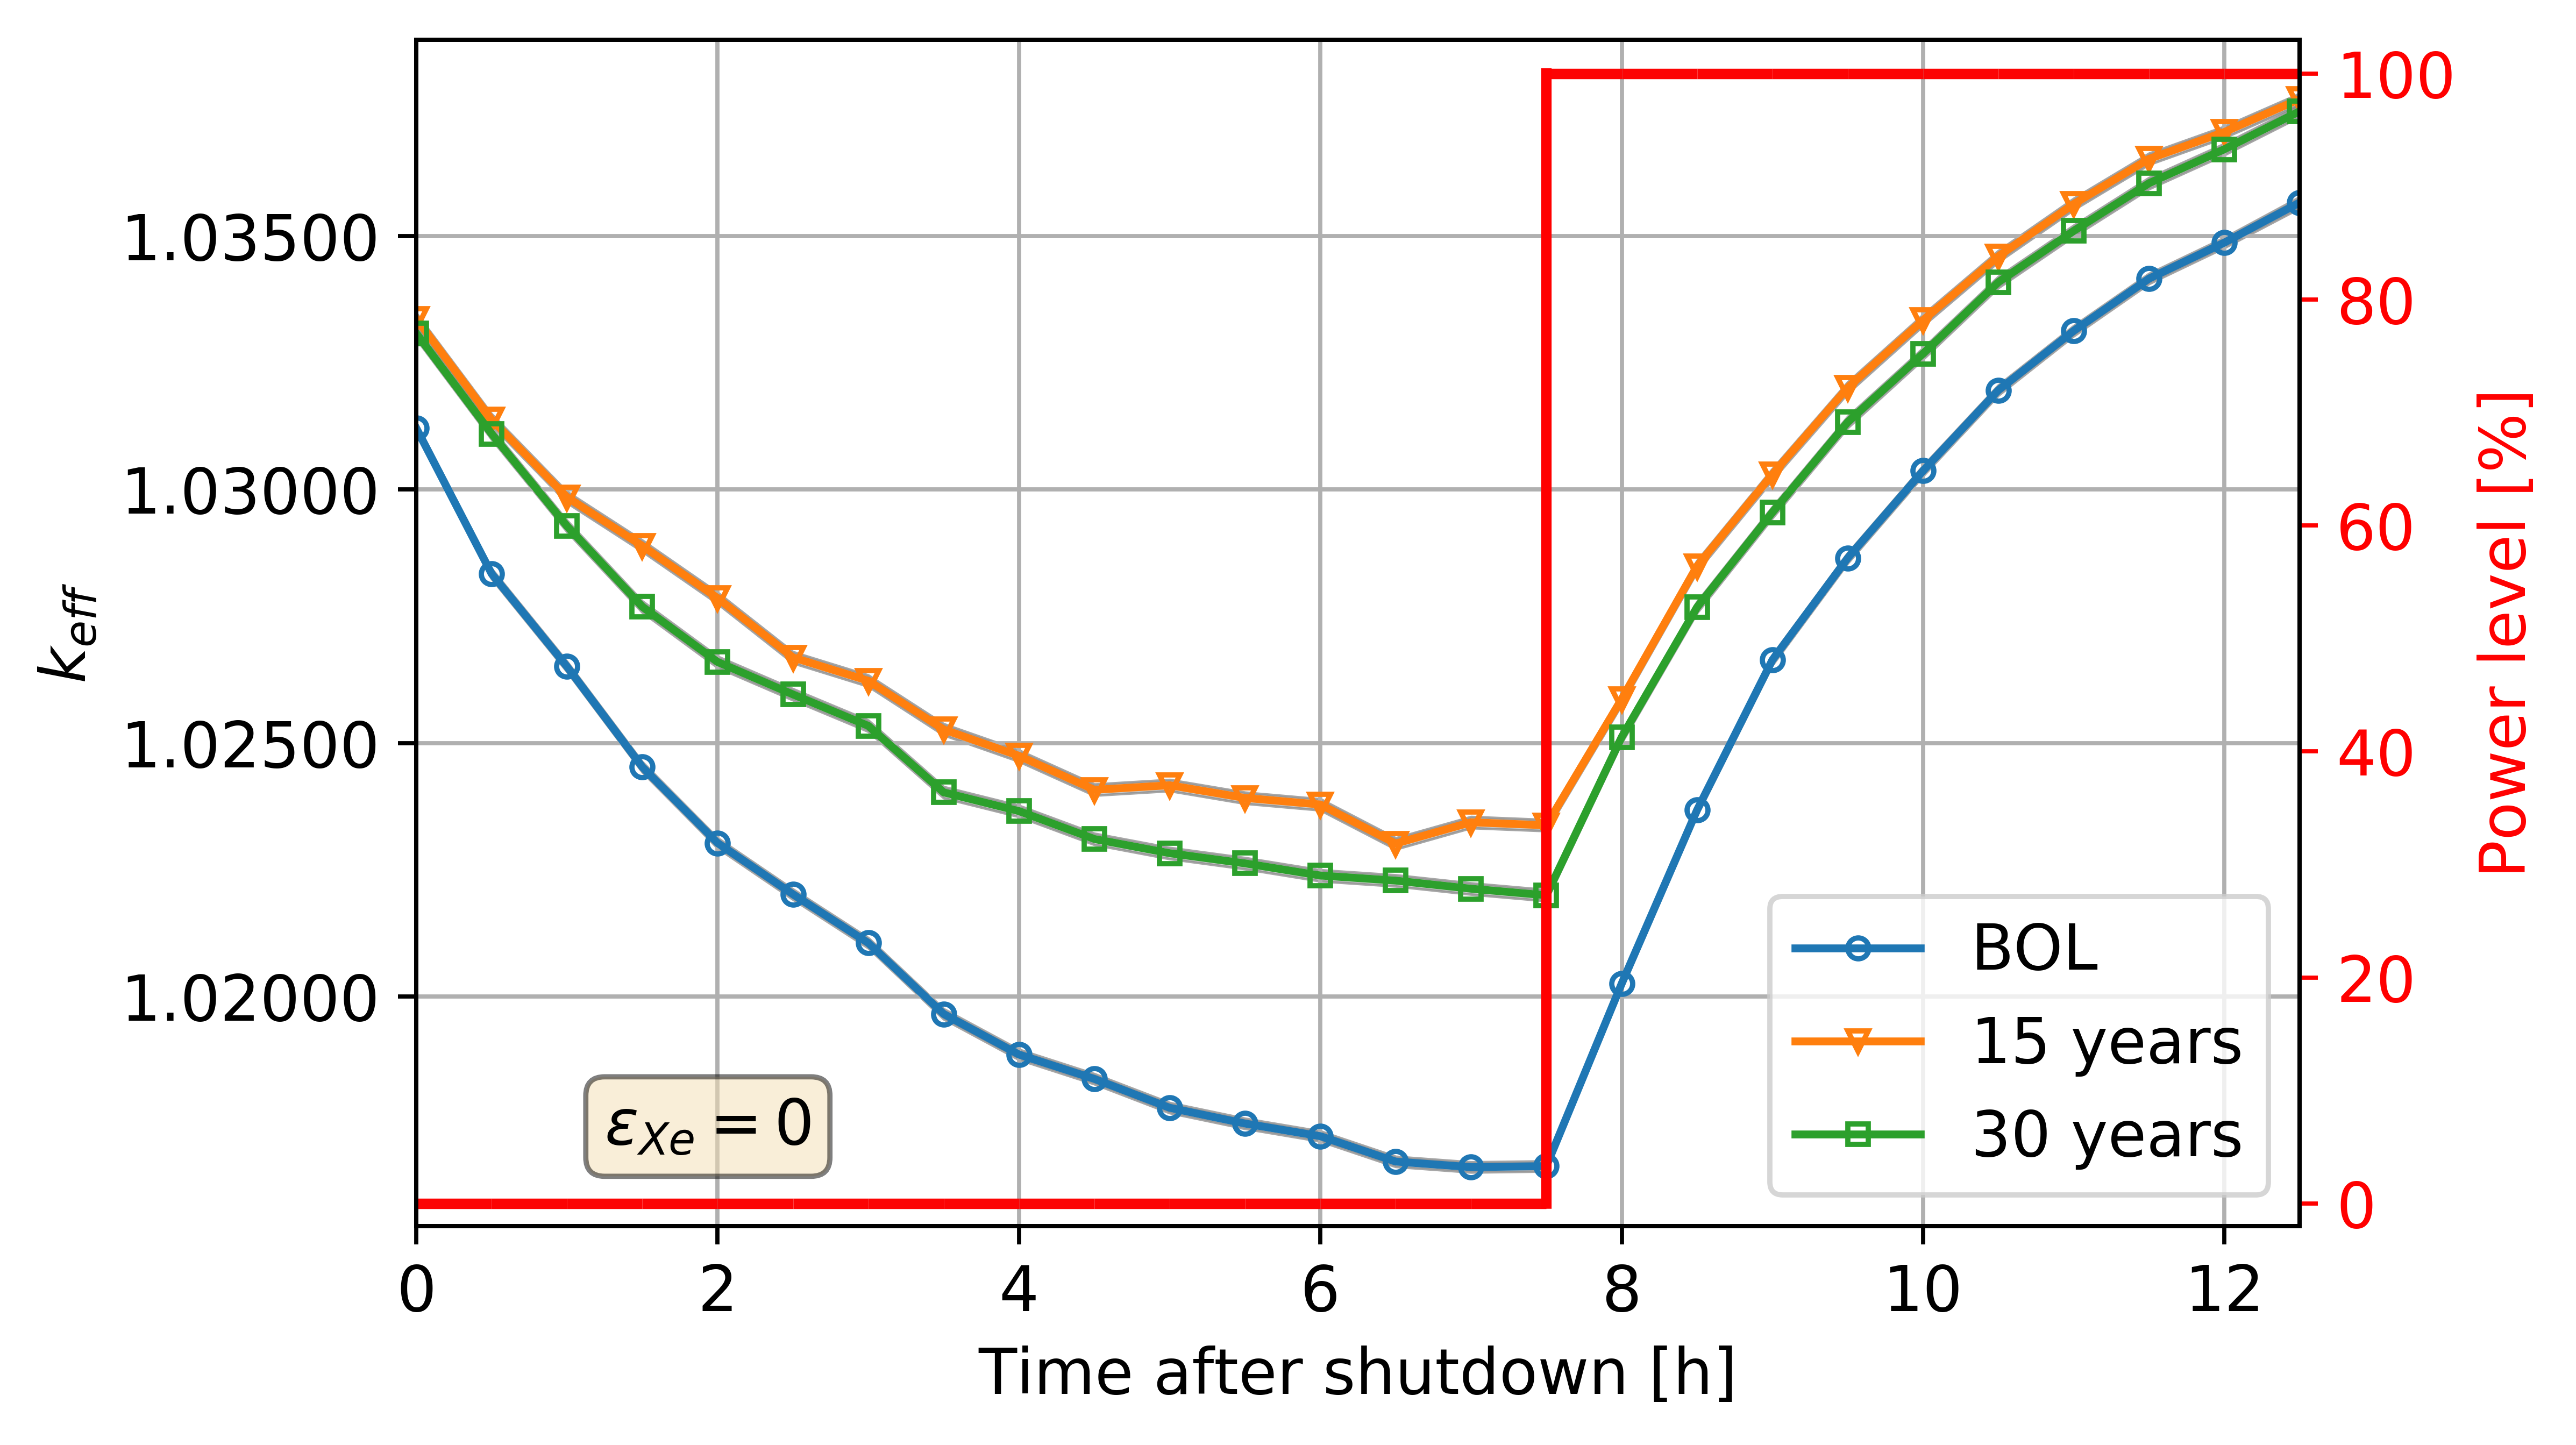
\includegraphics[width=0.92\textwidth]{ch6/kl1_keff.png}\vspace{-14mm}\\
	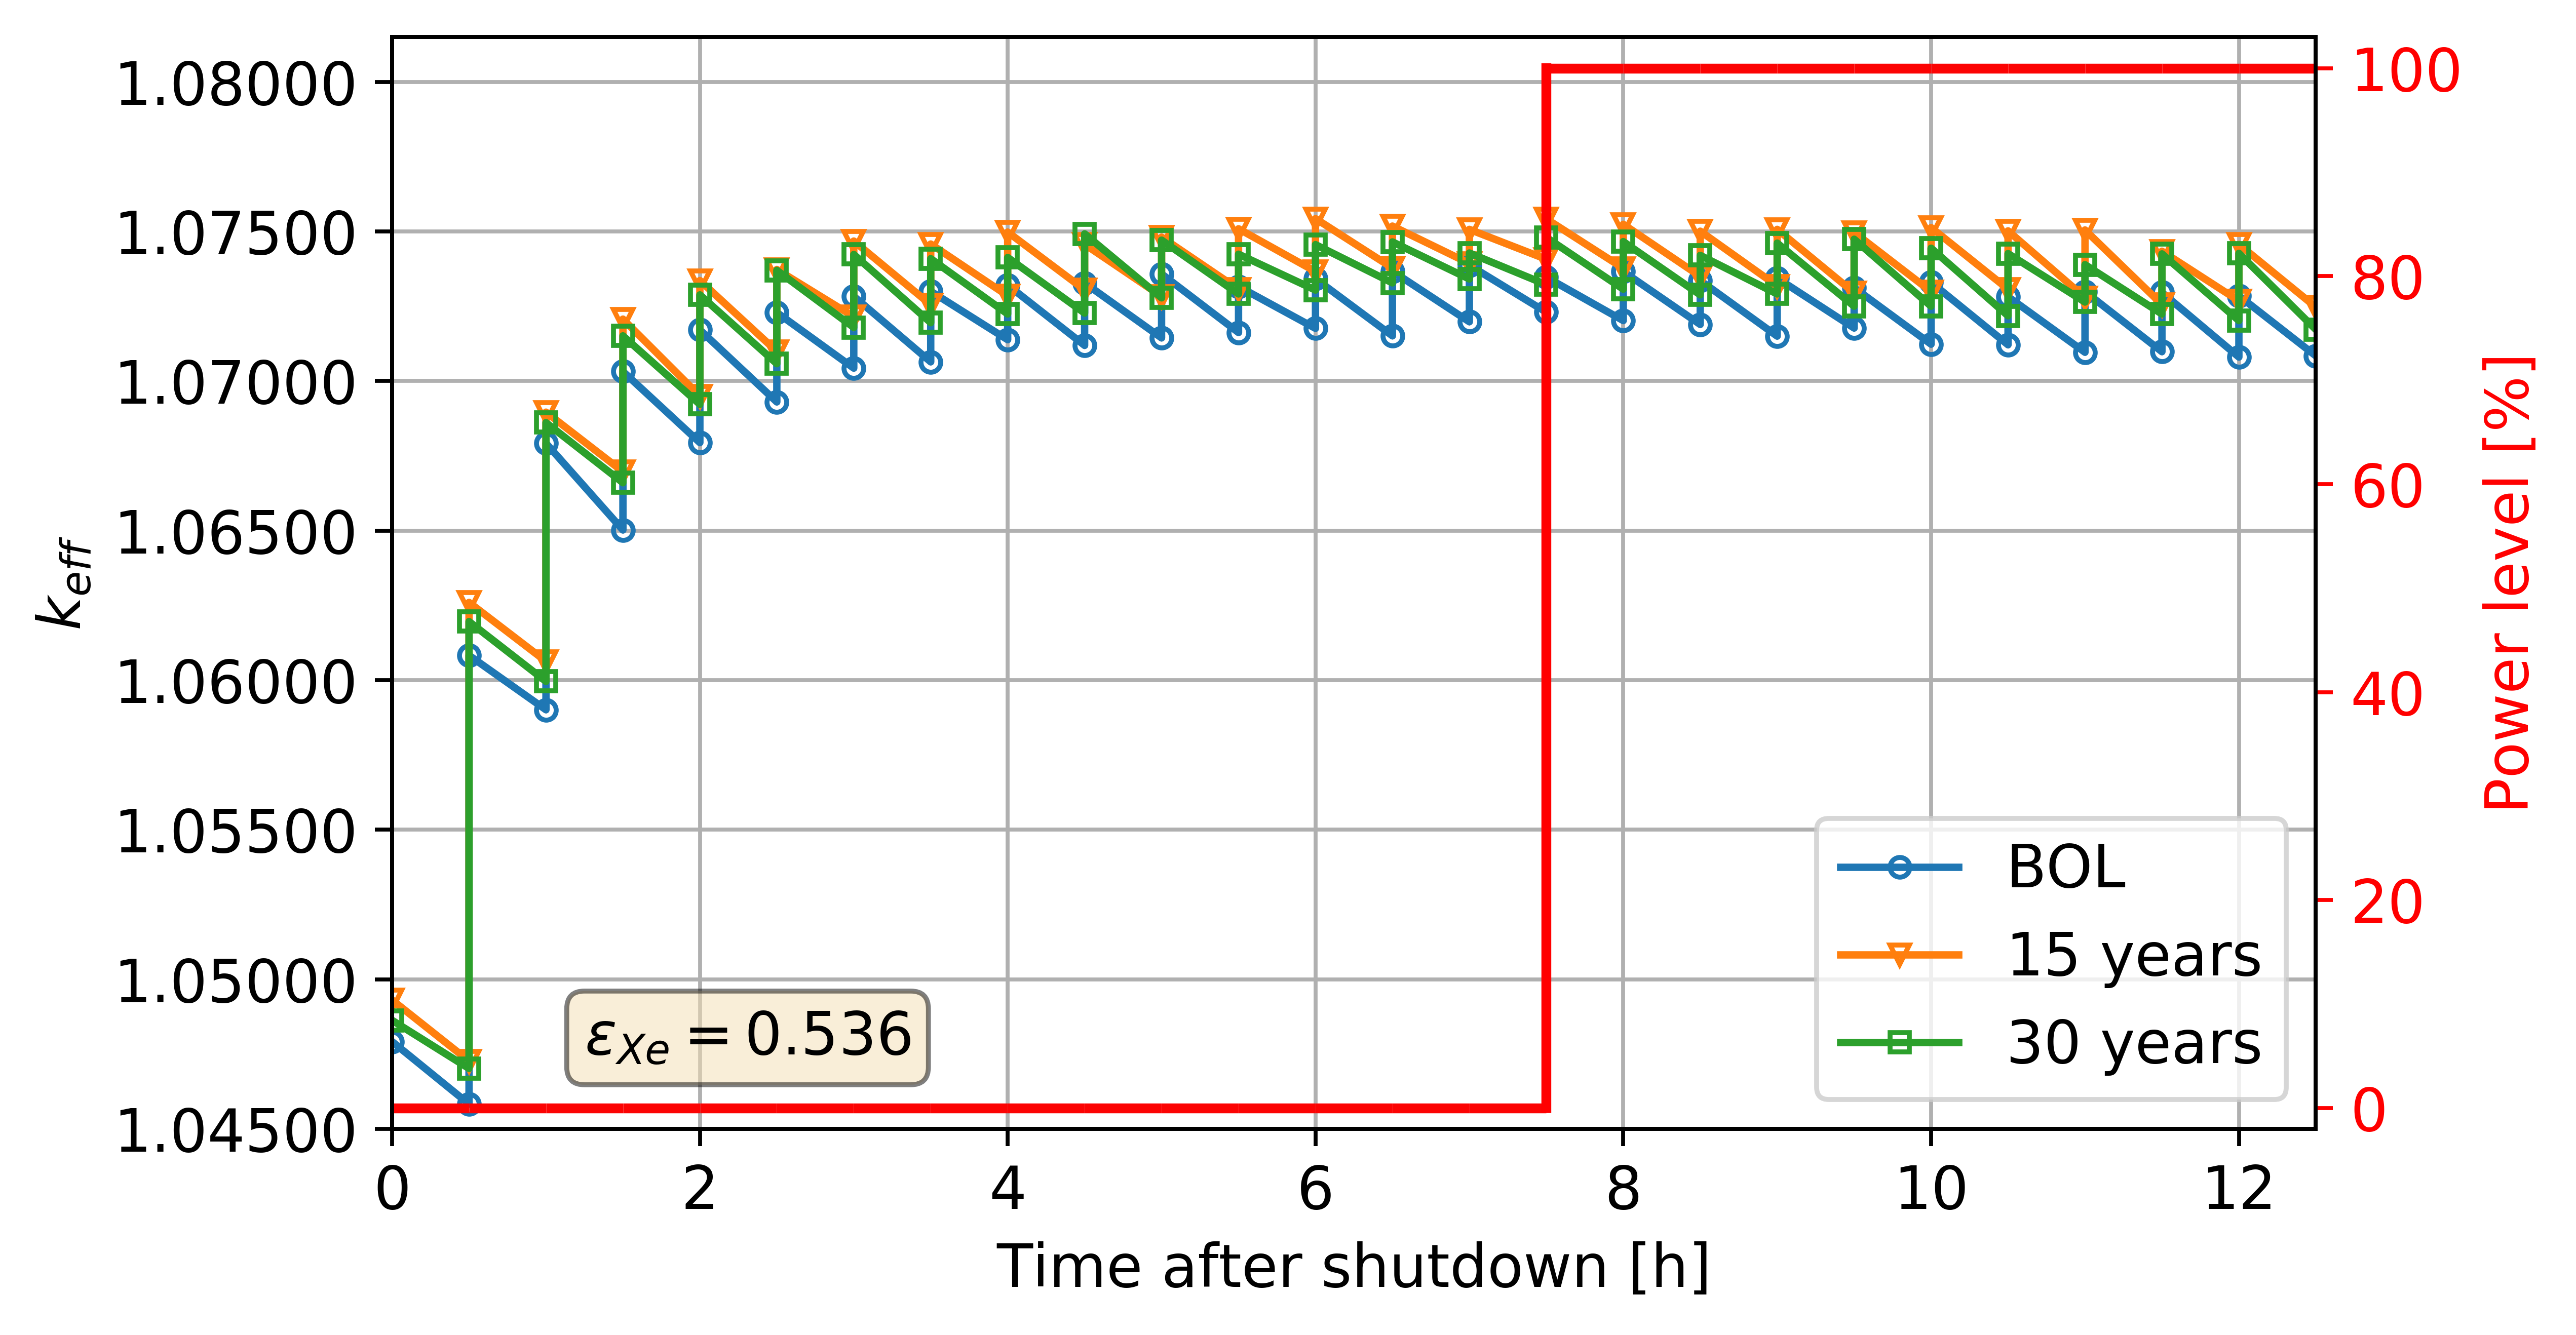
\includegraphics[width=0.905\textwidth]{ch6/kl25_keff.png}\vspace{-12mm}\\
	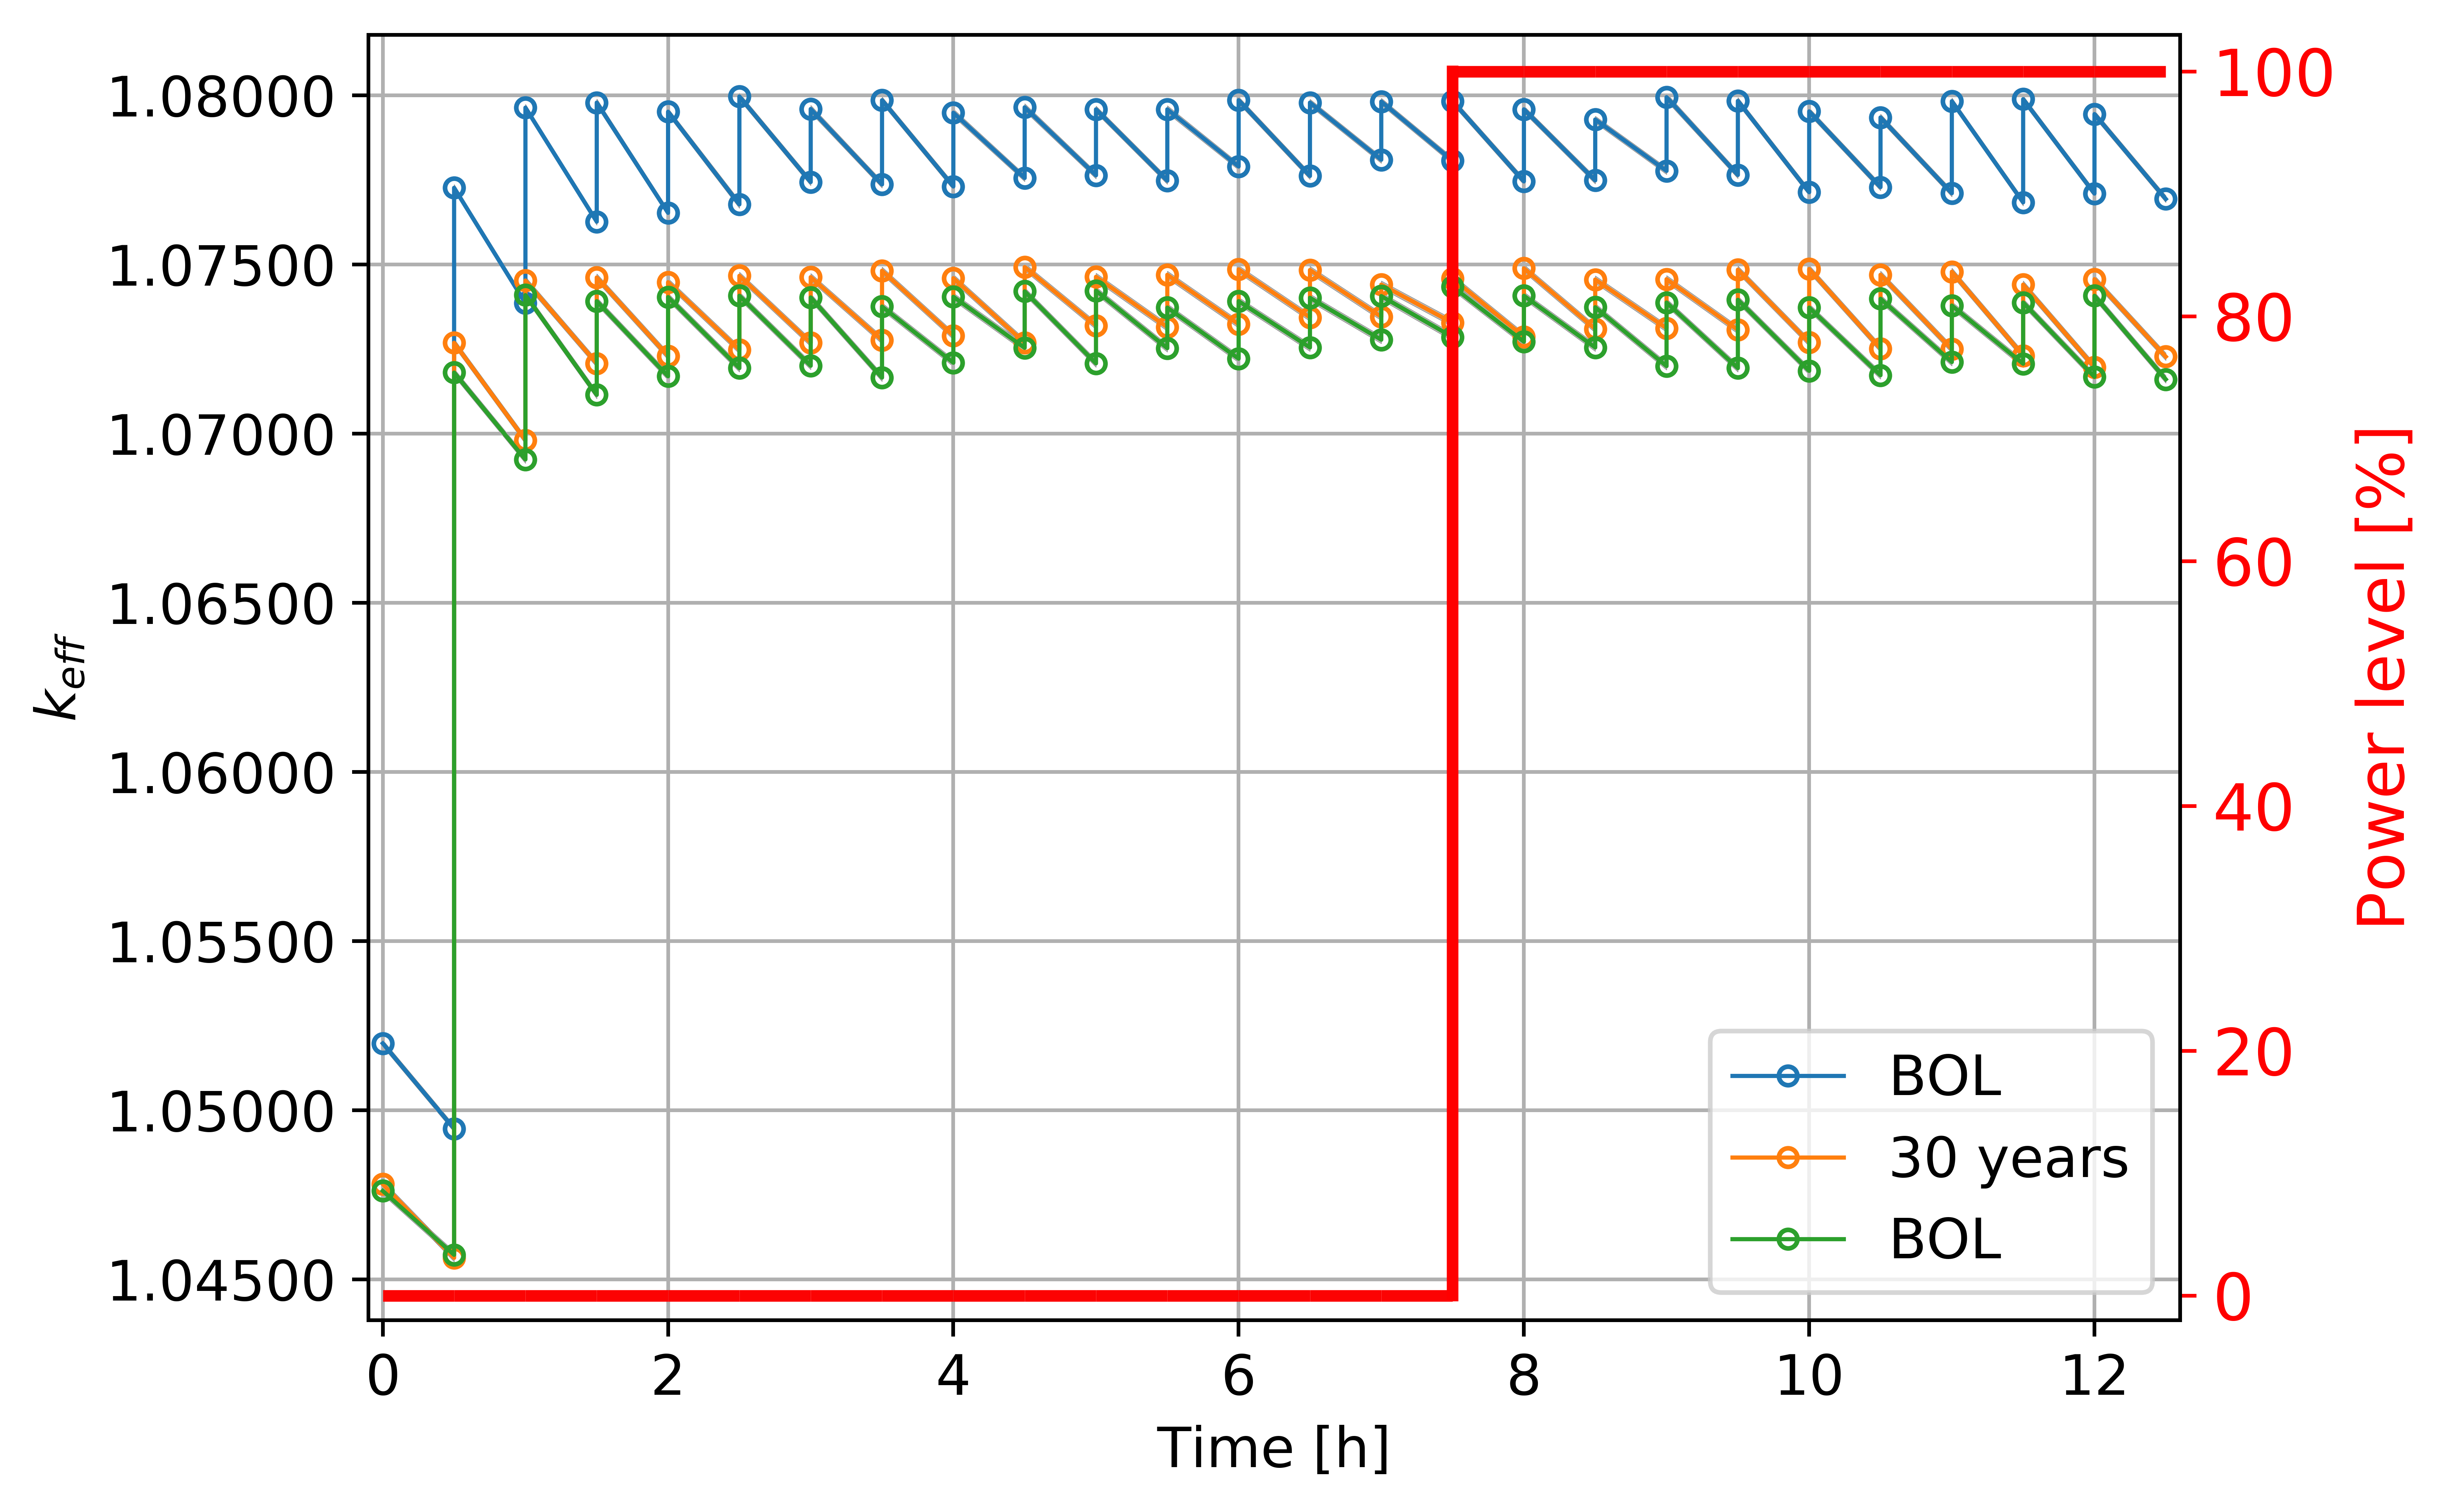
\includegraphics[width=0.905\textwidth]{ch6/kl100_keff.png}
\end{array}$
		\vspace{-5mm}
	\caption{SaltProc-calculated evolution of the effective multiplication 
	factor during the postulated load-following transient for various regimes 
	of the gas removal system operation. The uncertainty $\pm\sigma=10$ $pcm$ 
	is shaded.}
	\label{fig:msbr-lf-keff-evo}
\end{figure}

\begin{figure}[htbp!] % replace 't' with 'b' to 
	\centering
	$\begin{array}{r}
	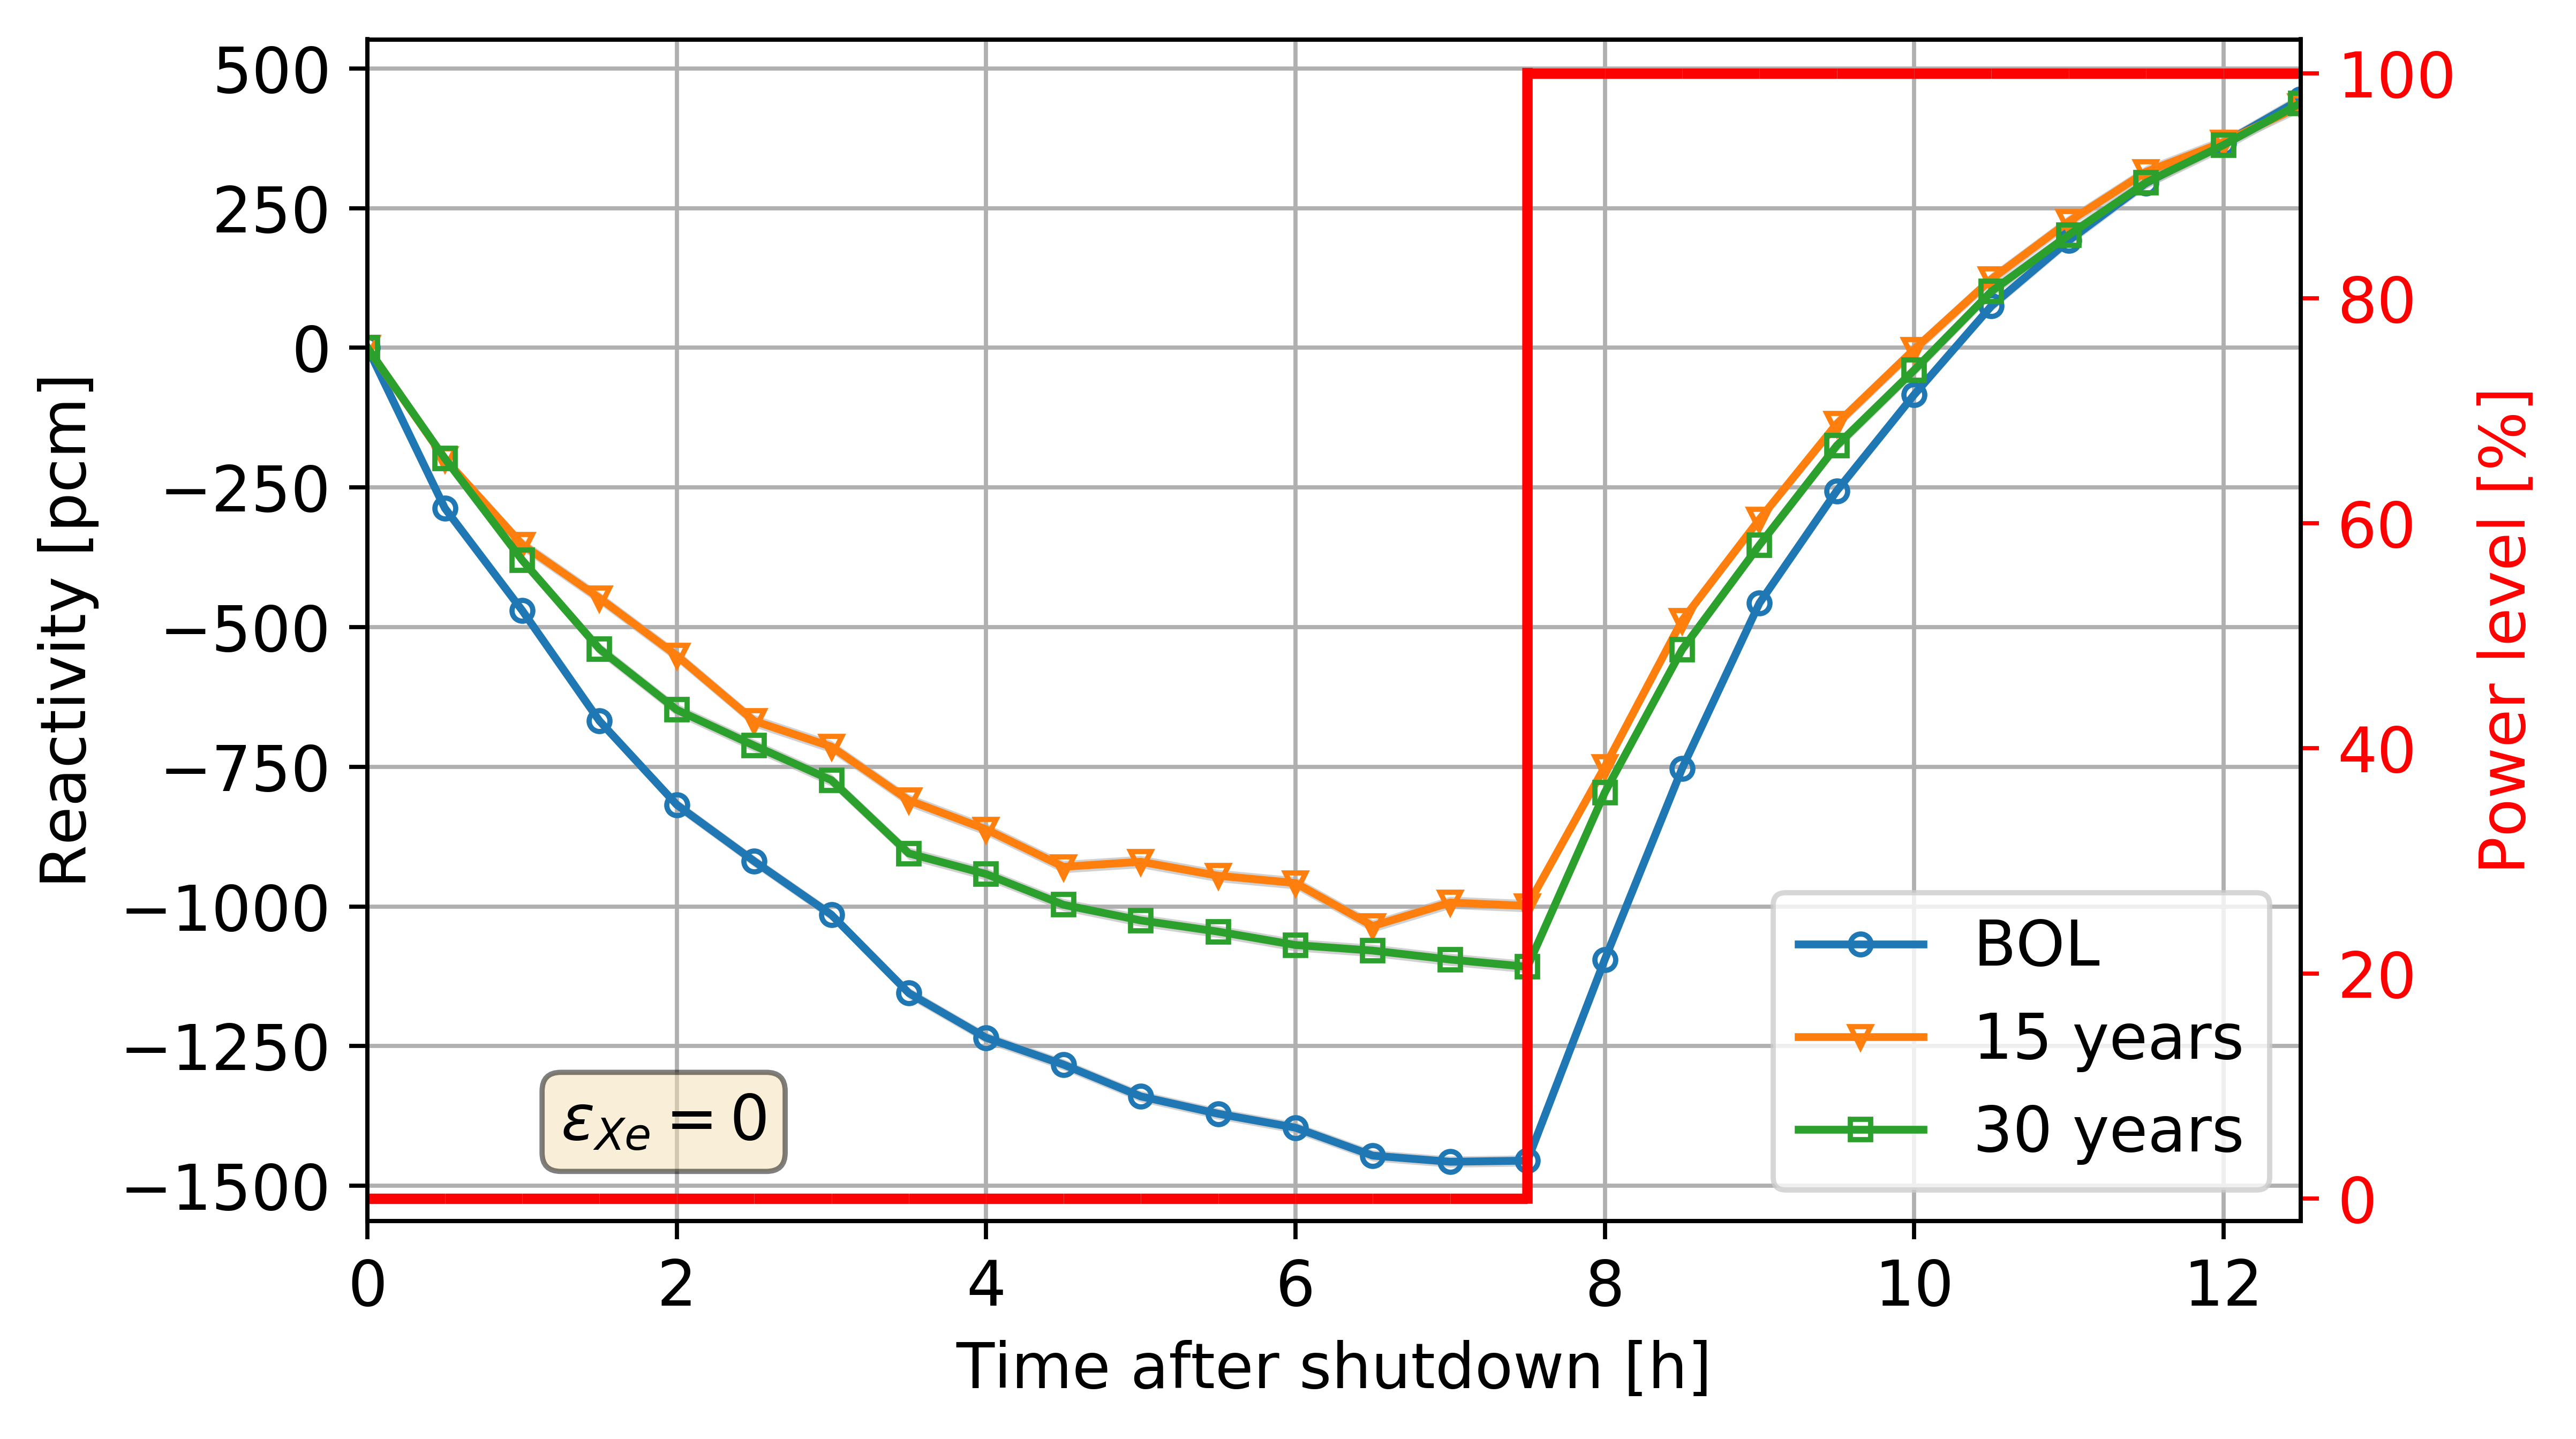
\includegraphics[width=0.923\textwidth]{ch6/kl1_rho.png}\vspace{-14mm}\\
	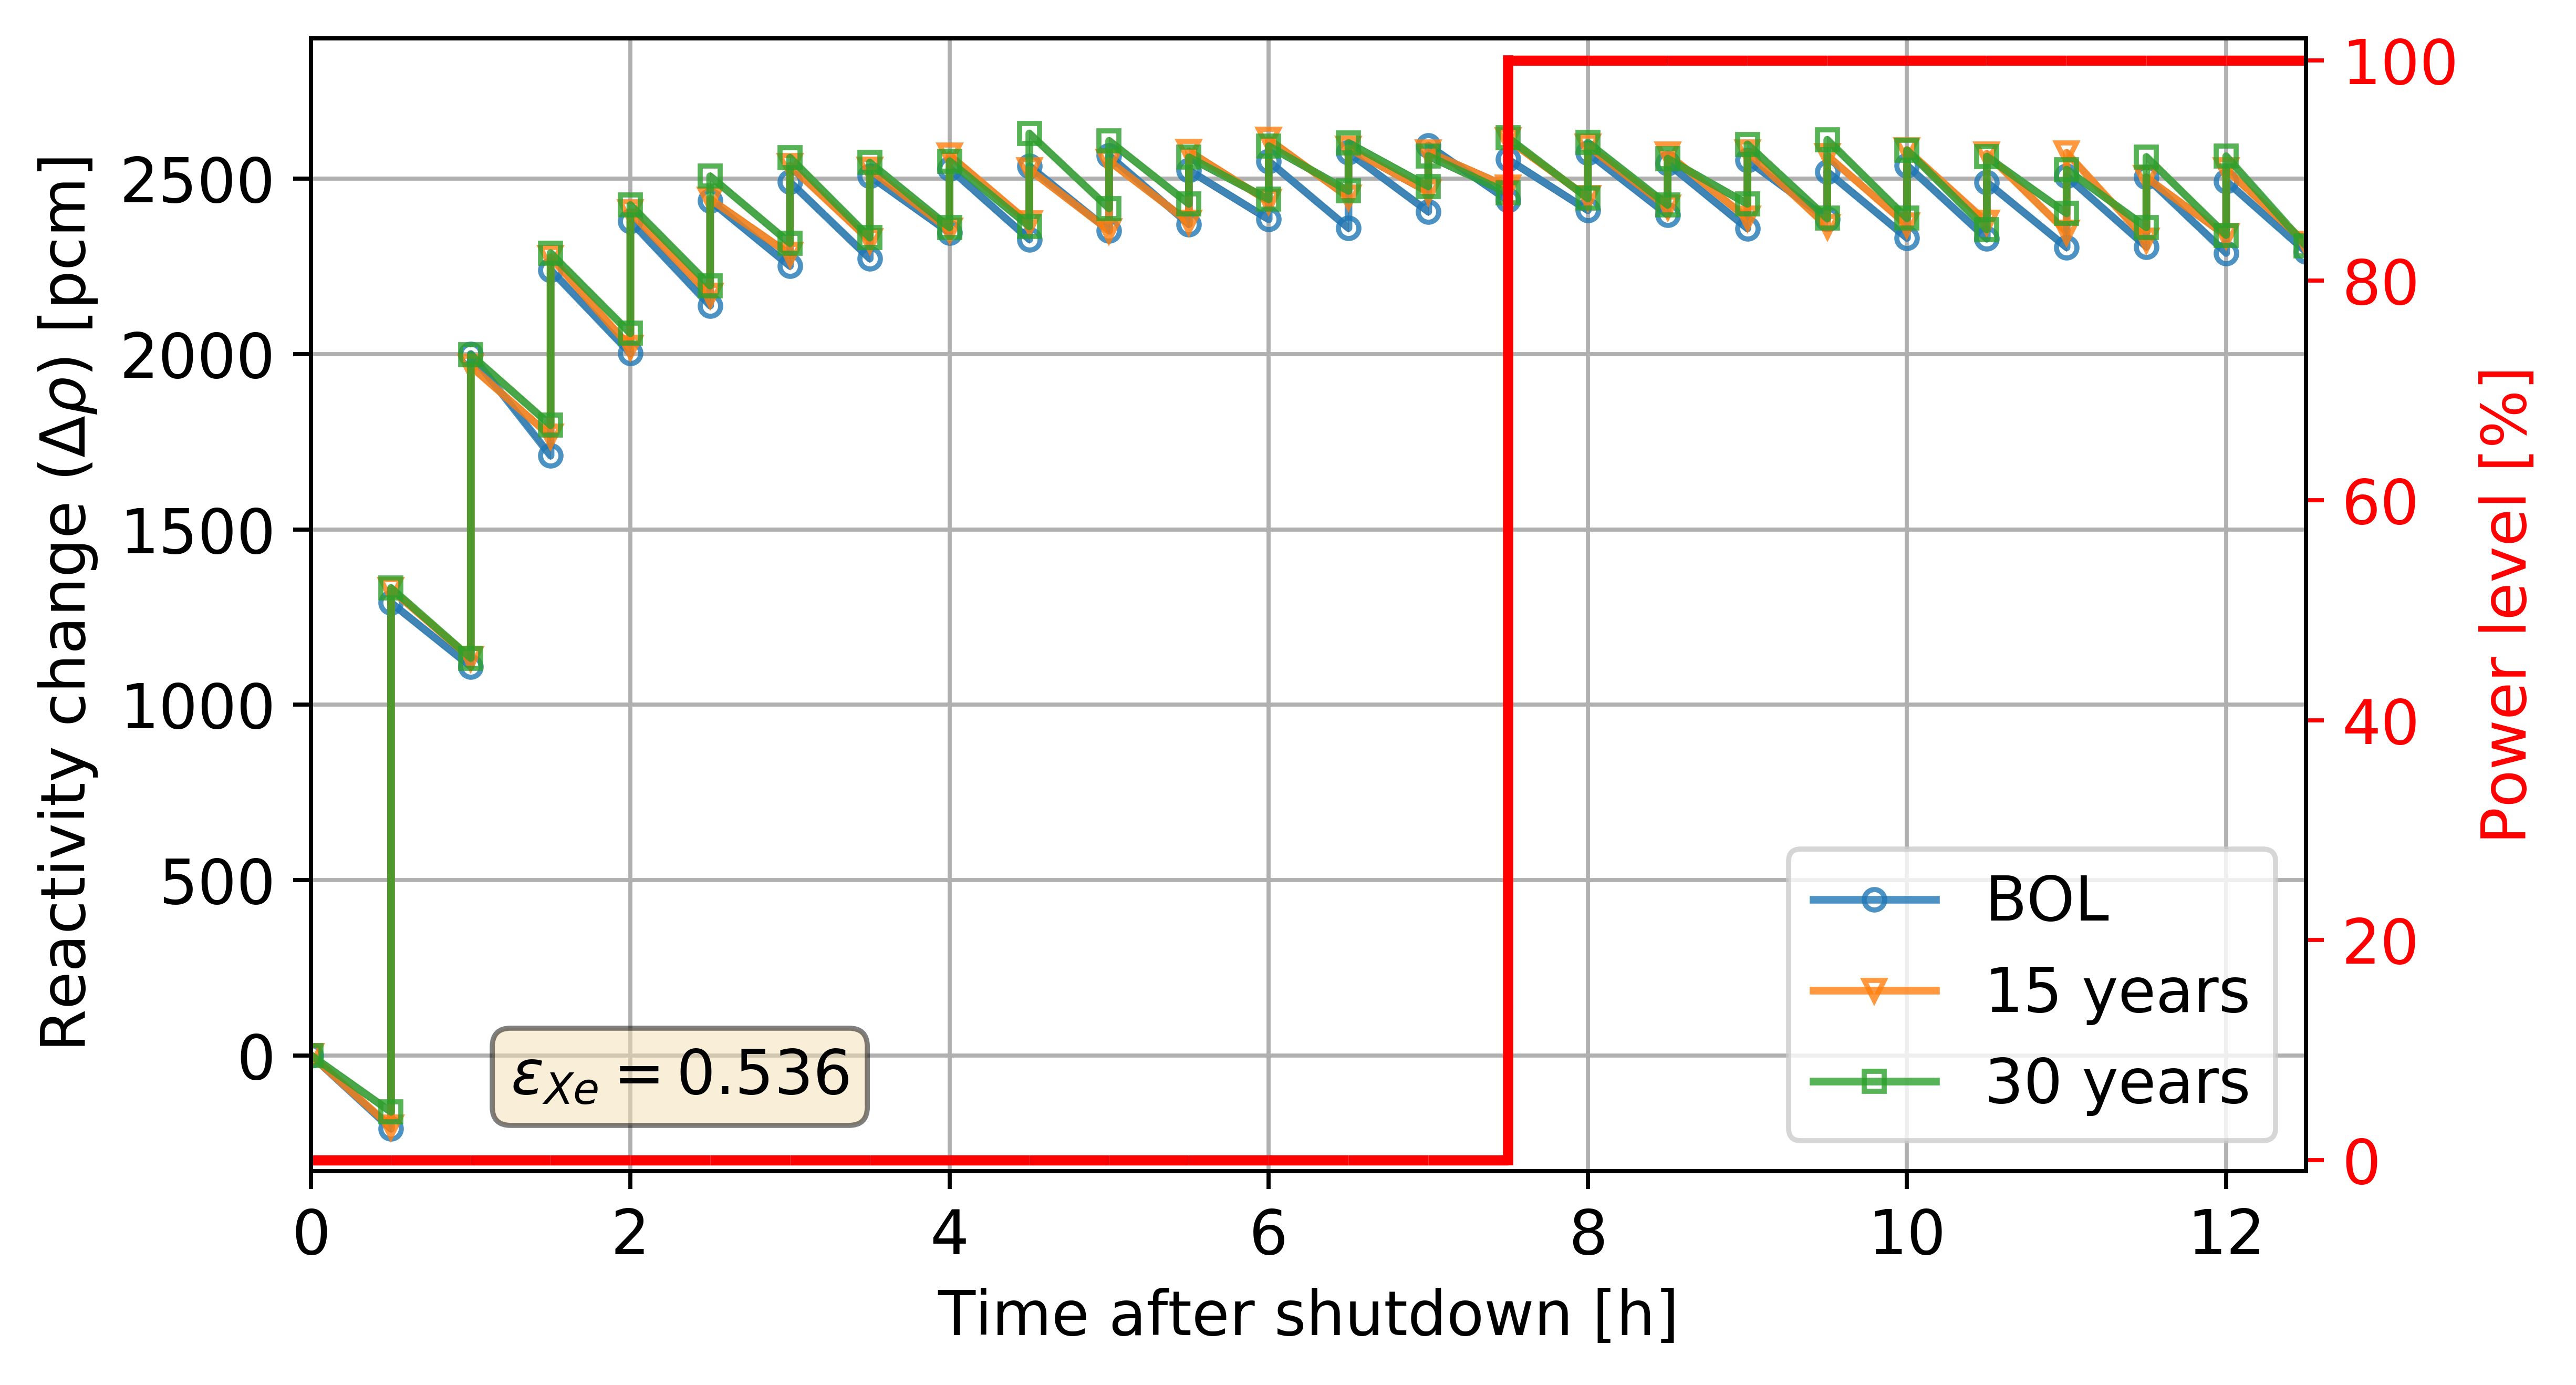
\includegraphics[width=0.9\textwidth]{ch6/kl25_rho.png}\vspace{-13mm}\\
	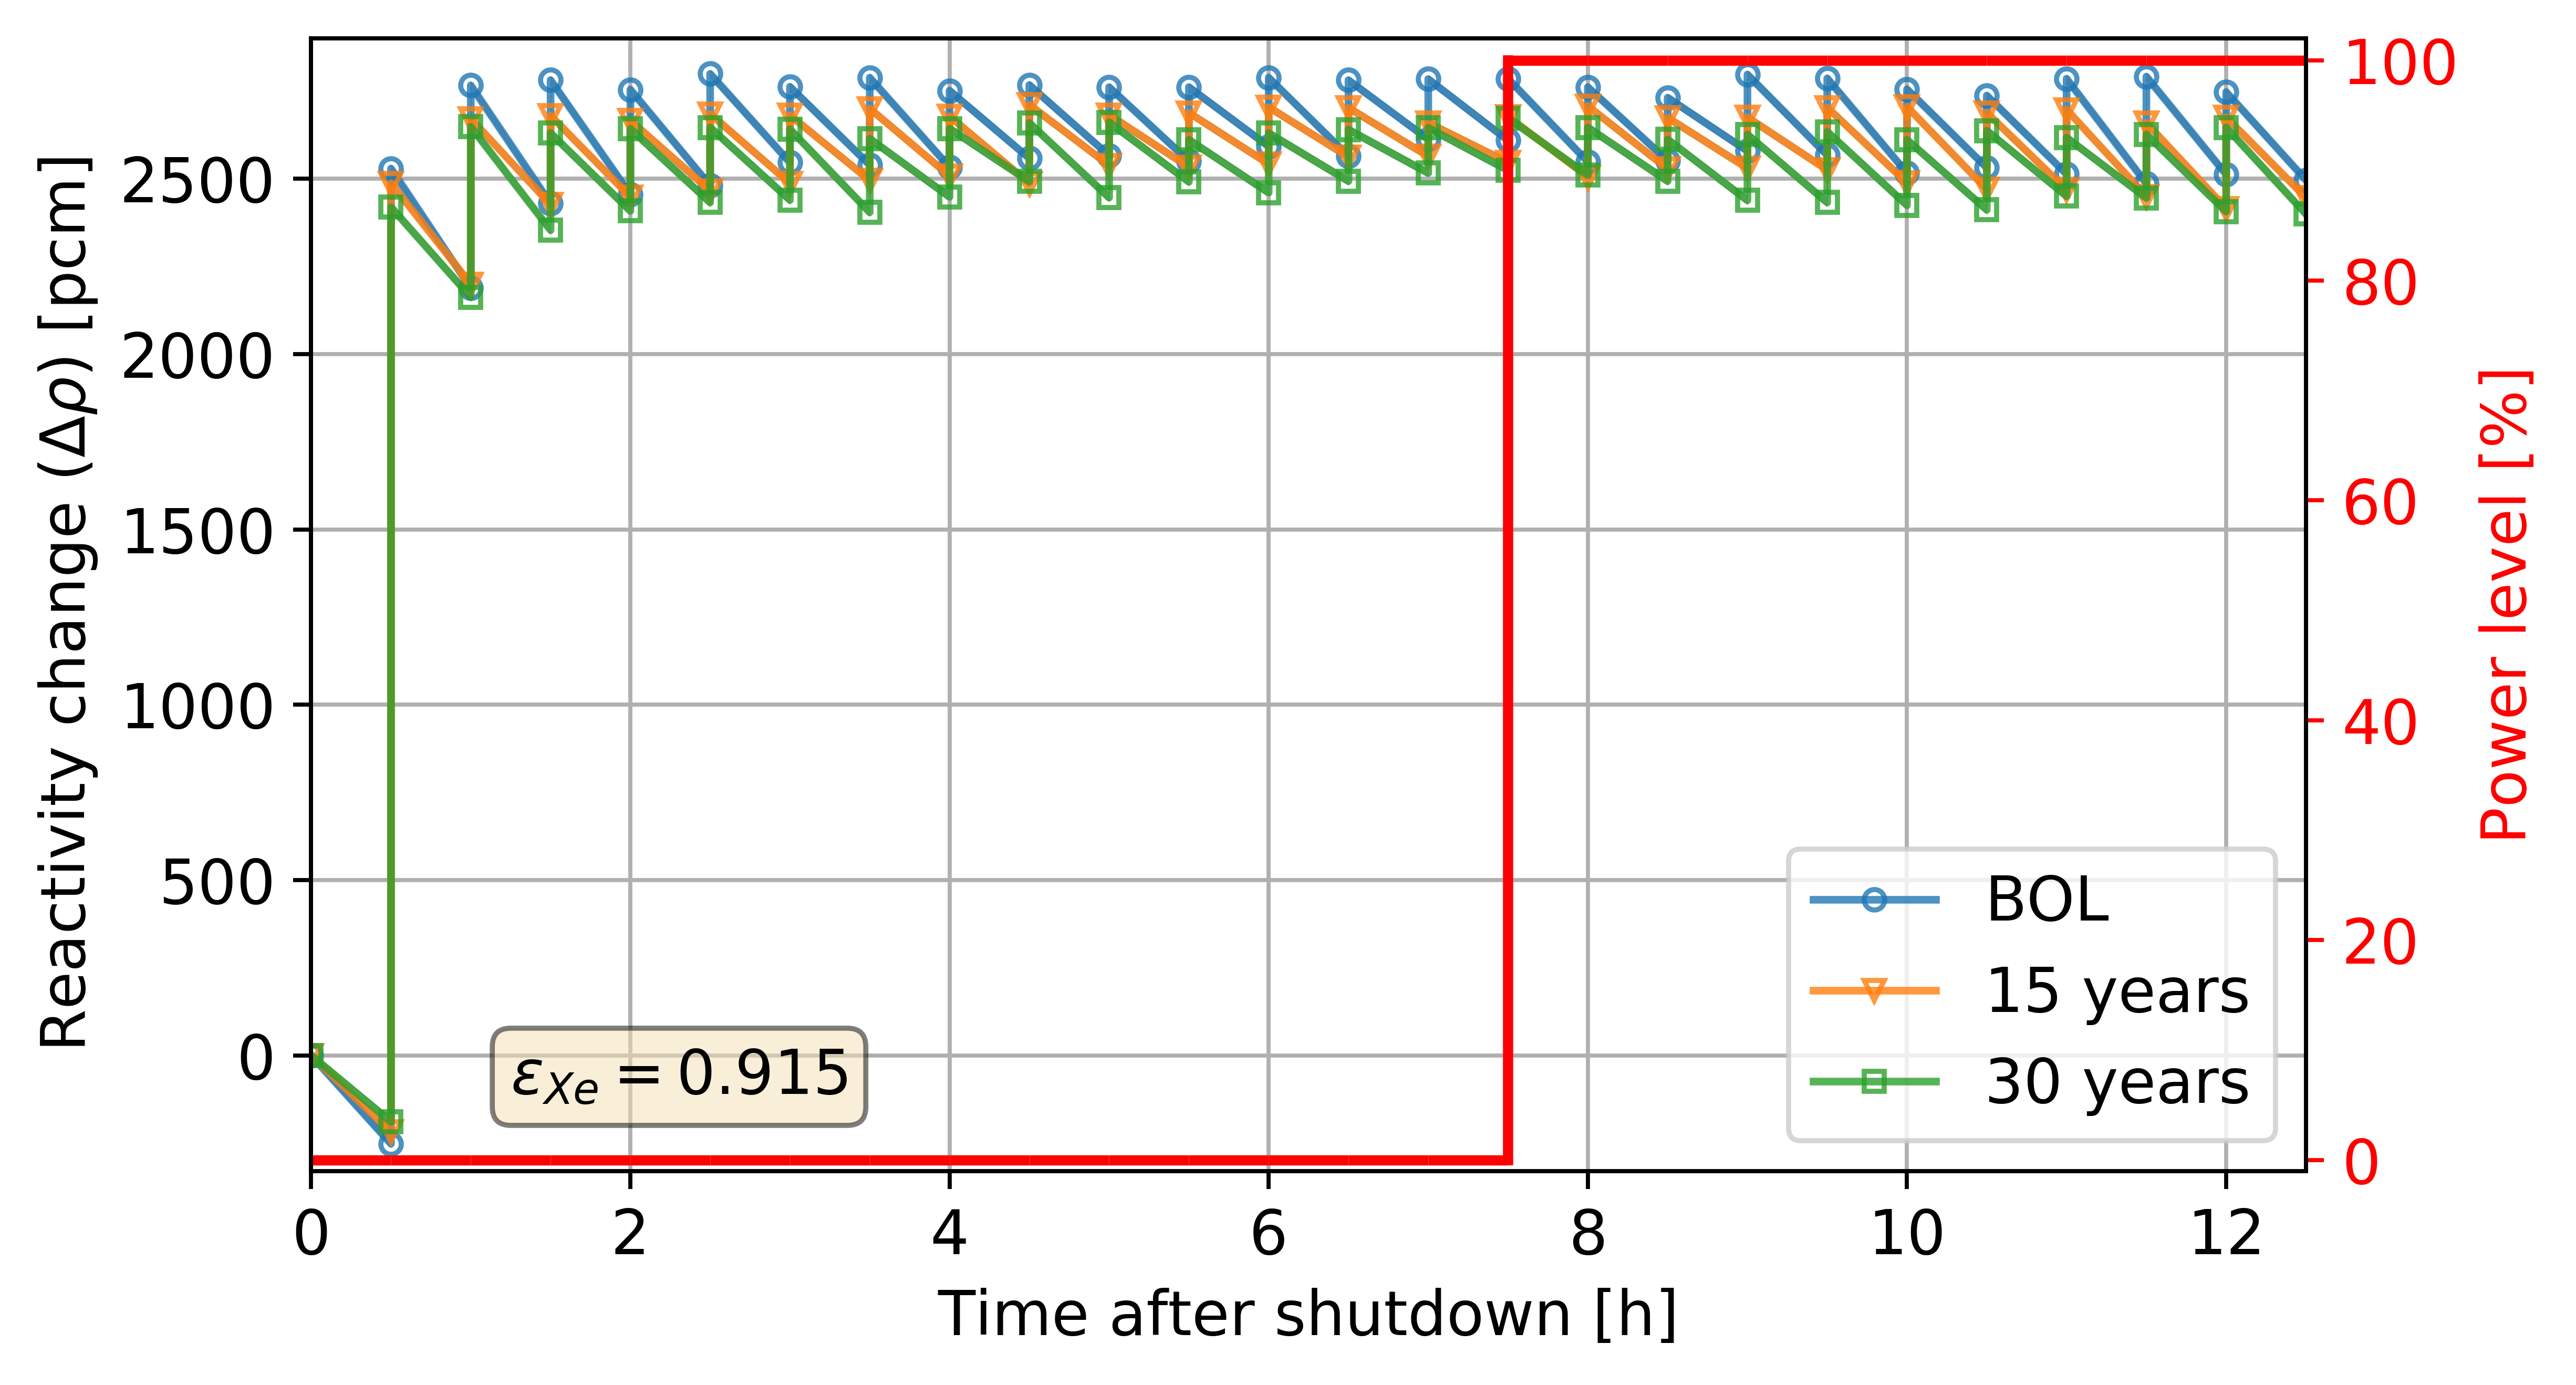
\includegraphics[width=0.9\textwidth]{ch6/kl100_rho.png}
	\end{array}$
	\vspace{-5mm}
	\caption{SaltProc-calculated evolution of the reactivity during the 
	postulated load-following transient for various regimes 
		of the gas removal system operation. The uncertainty $\pm\sigma=10$ 
		$pcm$ 
		is shaded.}
	\label{fig:msbr-lf-rho-evo}
\end{figure}
\FloatBarrier

\subsection{Fuel salt composition evolution}
Figure~\ref{fig:msbr-lf-xe-i-ratio} shows $^{135}$Xe and $^{135}$I mass 
dynamics evolution during the postulated transient for various gas removal 
efficiencies. The $^{135}$I/$^{135}$Xe concentration ratio at the beginning 
transient for the no-removal case is 2.45 and 2.03 at the \gls{BOL} and after 
30 years of full-power operation, respectively. The greater 
$^{135}$I/$^{135}$Xe concentration ratio at the startup leads to $^{135}$Xe 
concentration peak by 11\% higher than at the \gls{EOL} which is consistent 
with the \gls{TAP} \gls{MSR} results. However, larger $^{135}$Xe concentration 
does not necessary worsens the xenon poisoning effect 
(Figure~\ref{fig:msbr-lf-rho-evo}) because the spectrum hardens toward 
\gls{EOL} and $^{135}$Xe absorption cross section slumps with energy (see
Figure~\ref{fig:tap-pwr-spectrum}).

For the high gas removal efficiency regime, the $^{135}$I/$^{135}$Xe 
concentration ratio is 2.47 and 2.08 at the \gls{BOL} and after 
30 years of full-power operation, respectively. For the \gls{BOL} and 
\gls{EOL}, the $^{135}$Xe concentration peaked only by 8\% at the end of a 
first 30-minute depletion step which caused a 189-$pcm$ negative reactivity 
insertion. Afterward, the concentration of $^{135}$Xe dropped quickly because 
the gas removal system extracted most of the fission gas. The $^{135}$Xe 
concentration in the fuel salt before the shutdown is approximately 7 times 
greater than after the power turned back on, which caused significant 
reactivity growth by $\approx2550$ $pcm$. Surprisingly, the removal of 12 g of 
$^{135}$Xe from $t=30min$ to $t=60min$ caused an impressive 2600-$pcm$ 
positive reactivity insertion (217 pcm/g$^{135}$Xe reactivity worth). 
\begin{figure}[htbp!] % replace 't' with 'b' to 
	\centering
	$\begin{array}{r}
	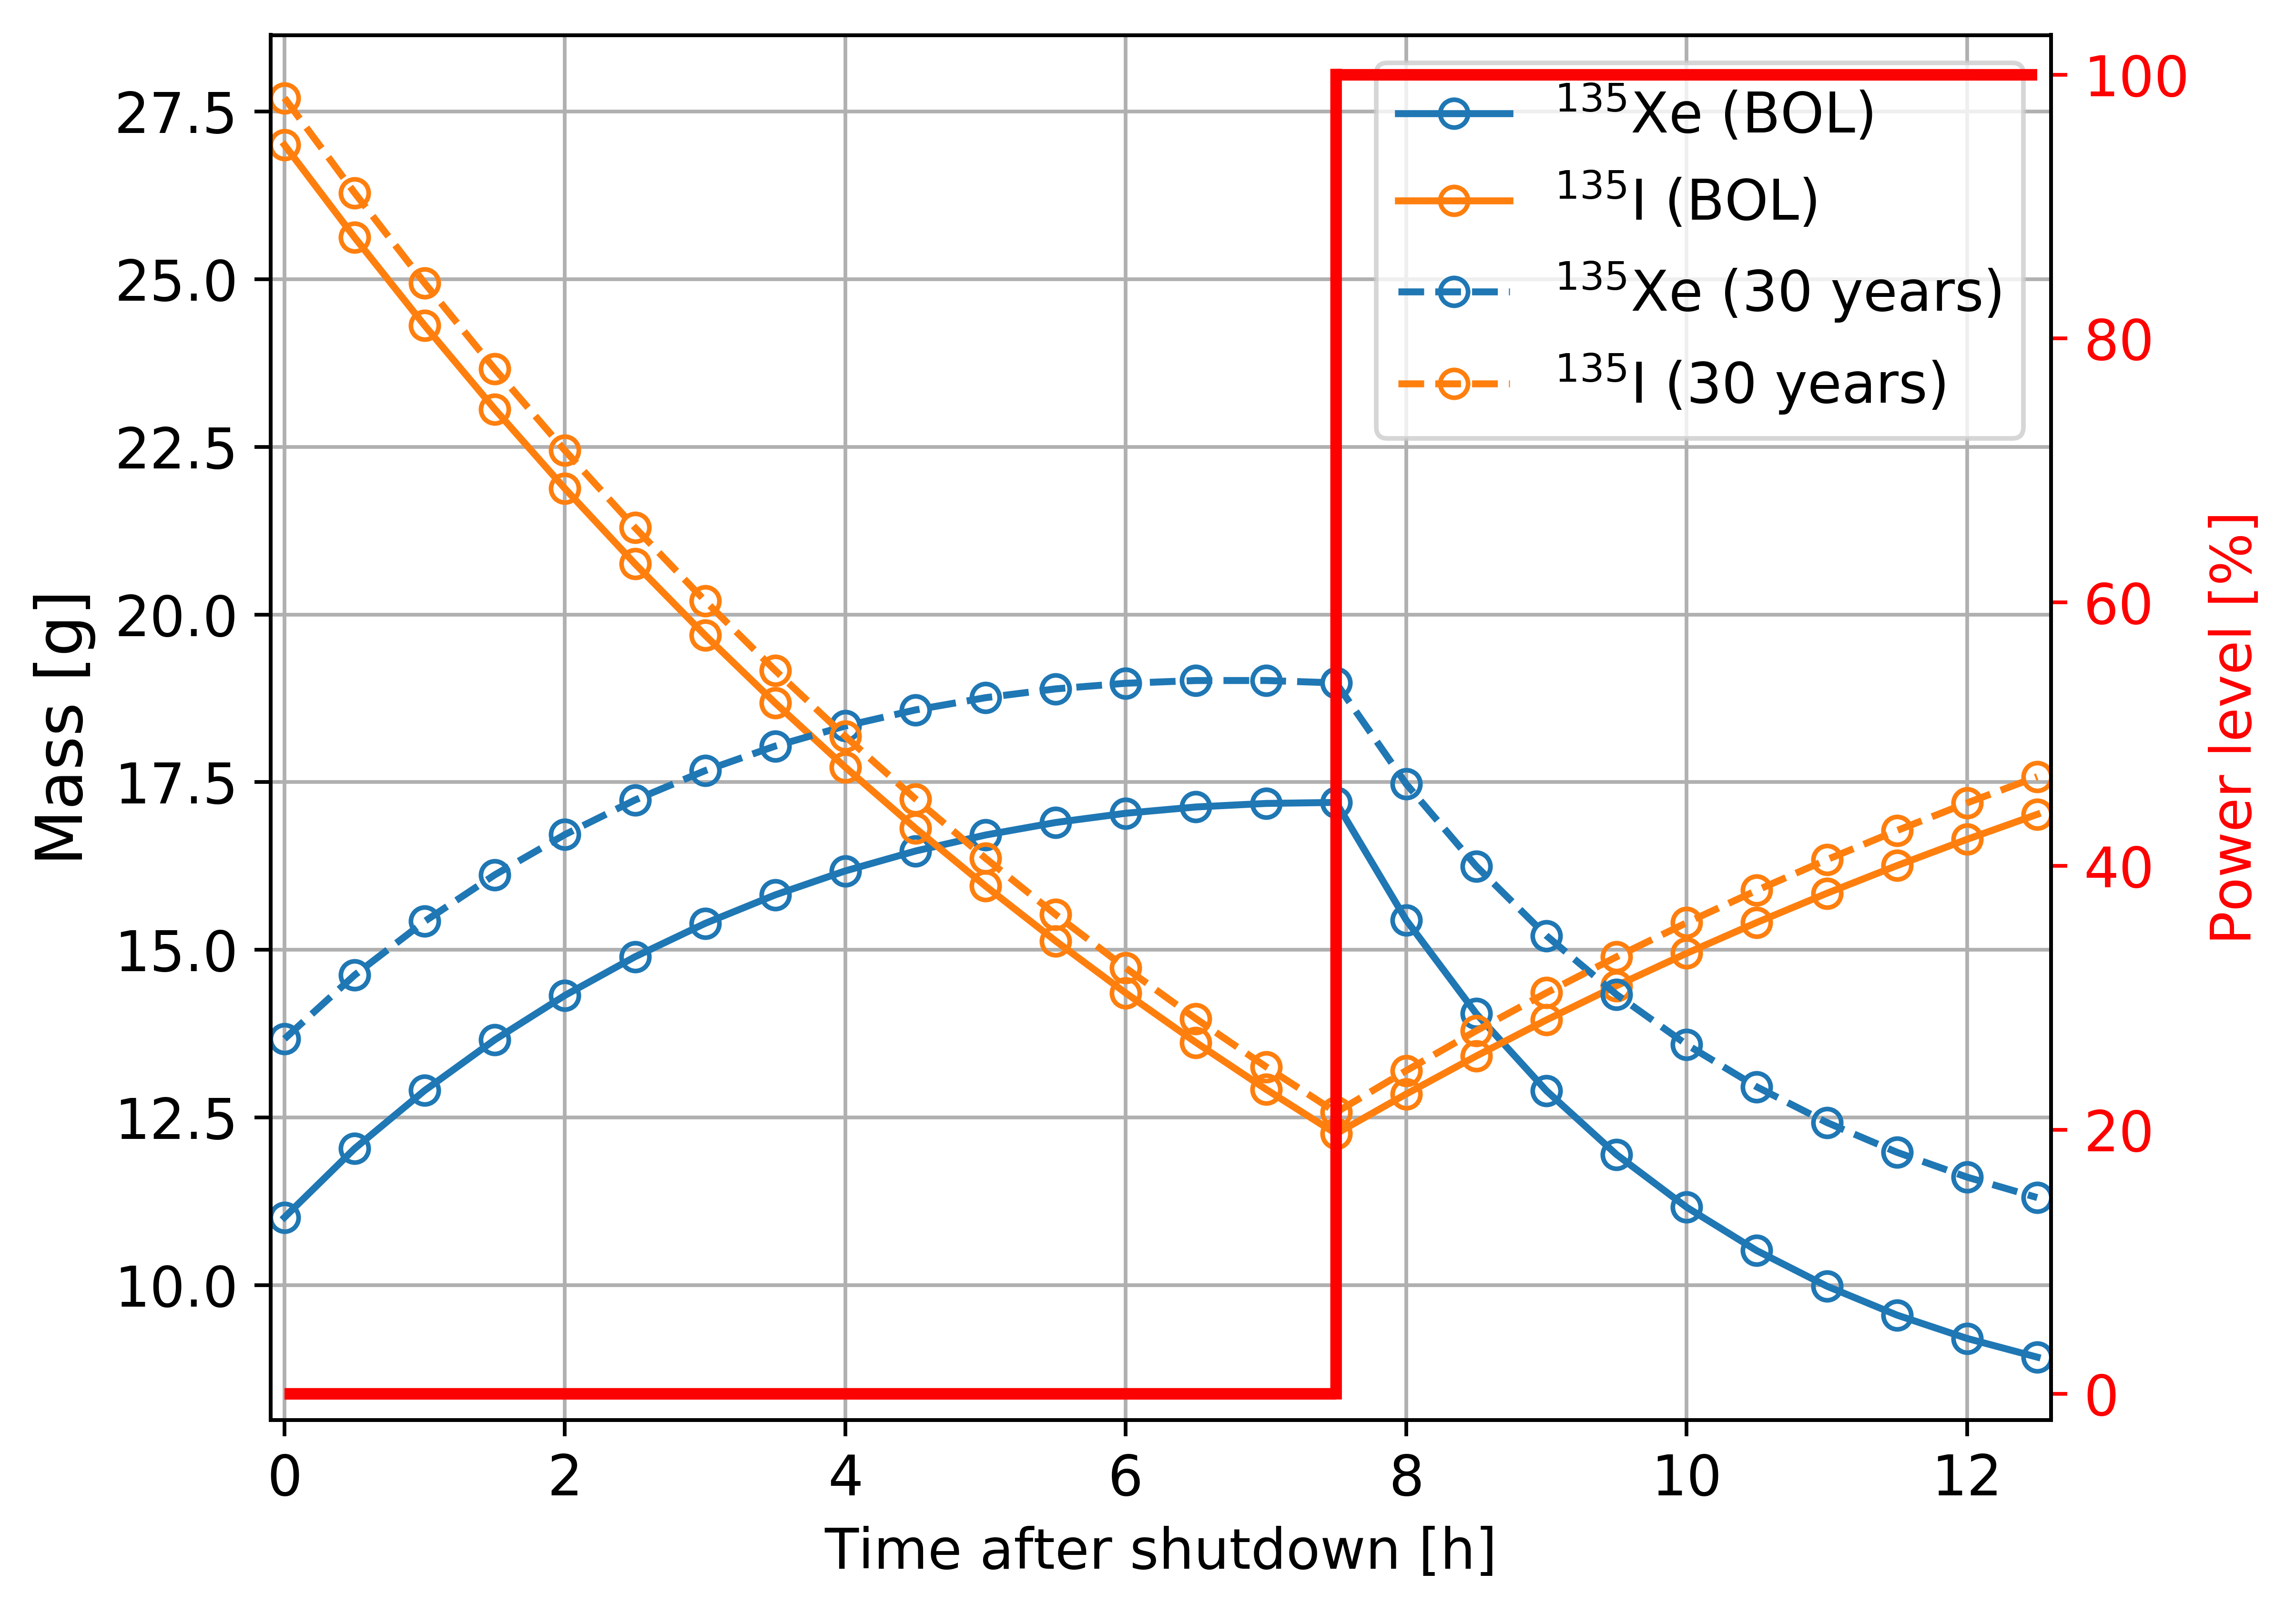
\includegraphics[width=0.88\textwidth]{ch6/kl1_xe_i_ratio.png}\vspace{-13mm}\\
	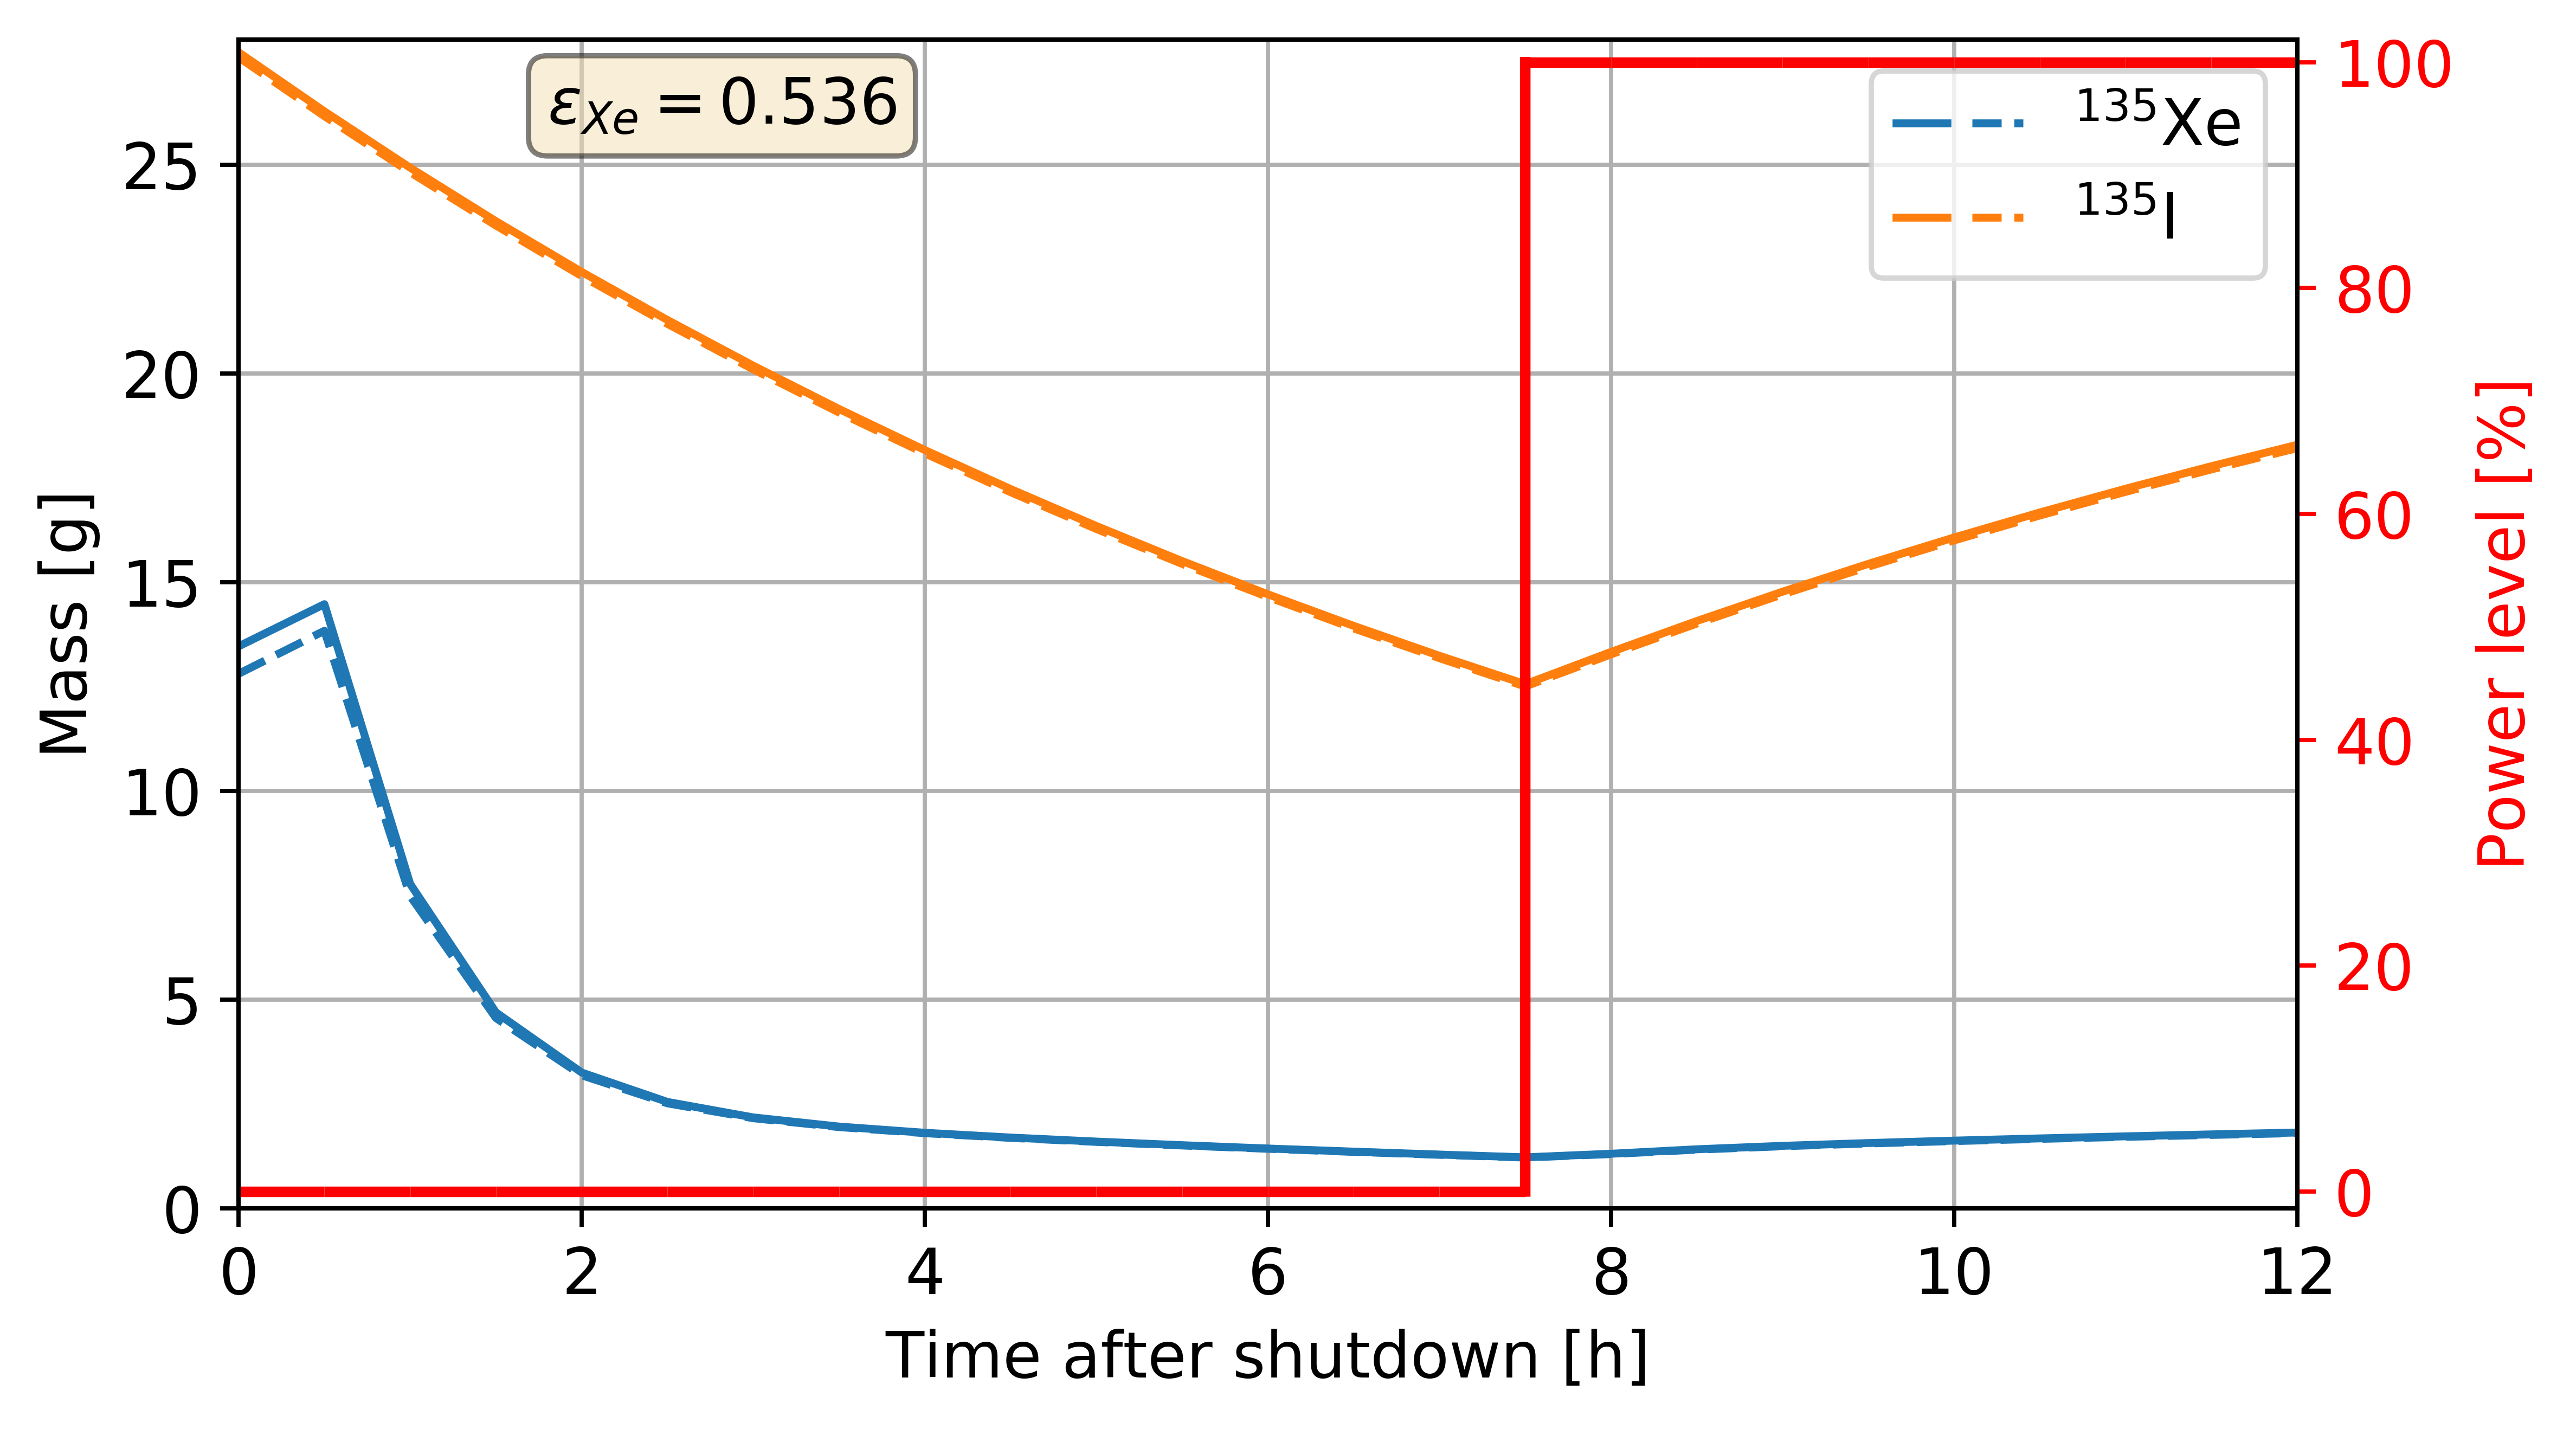
\includegraphics[width=0.88\textwidth]{ch6/kl25_xe_i_ratio.png}\vspace{-13mm}\\
	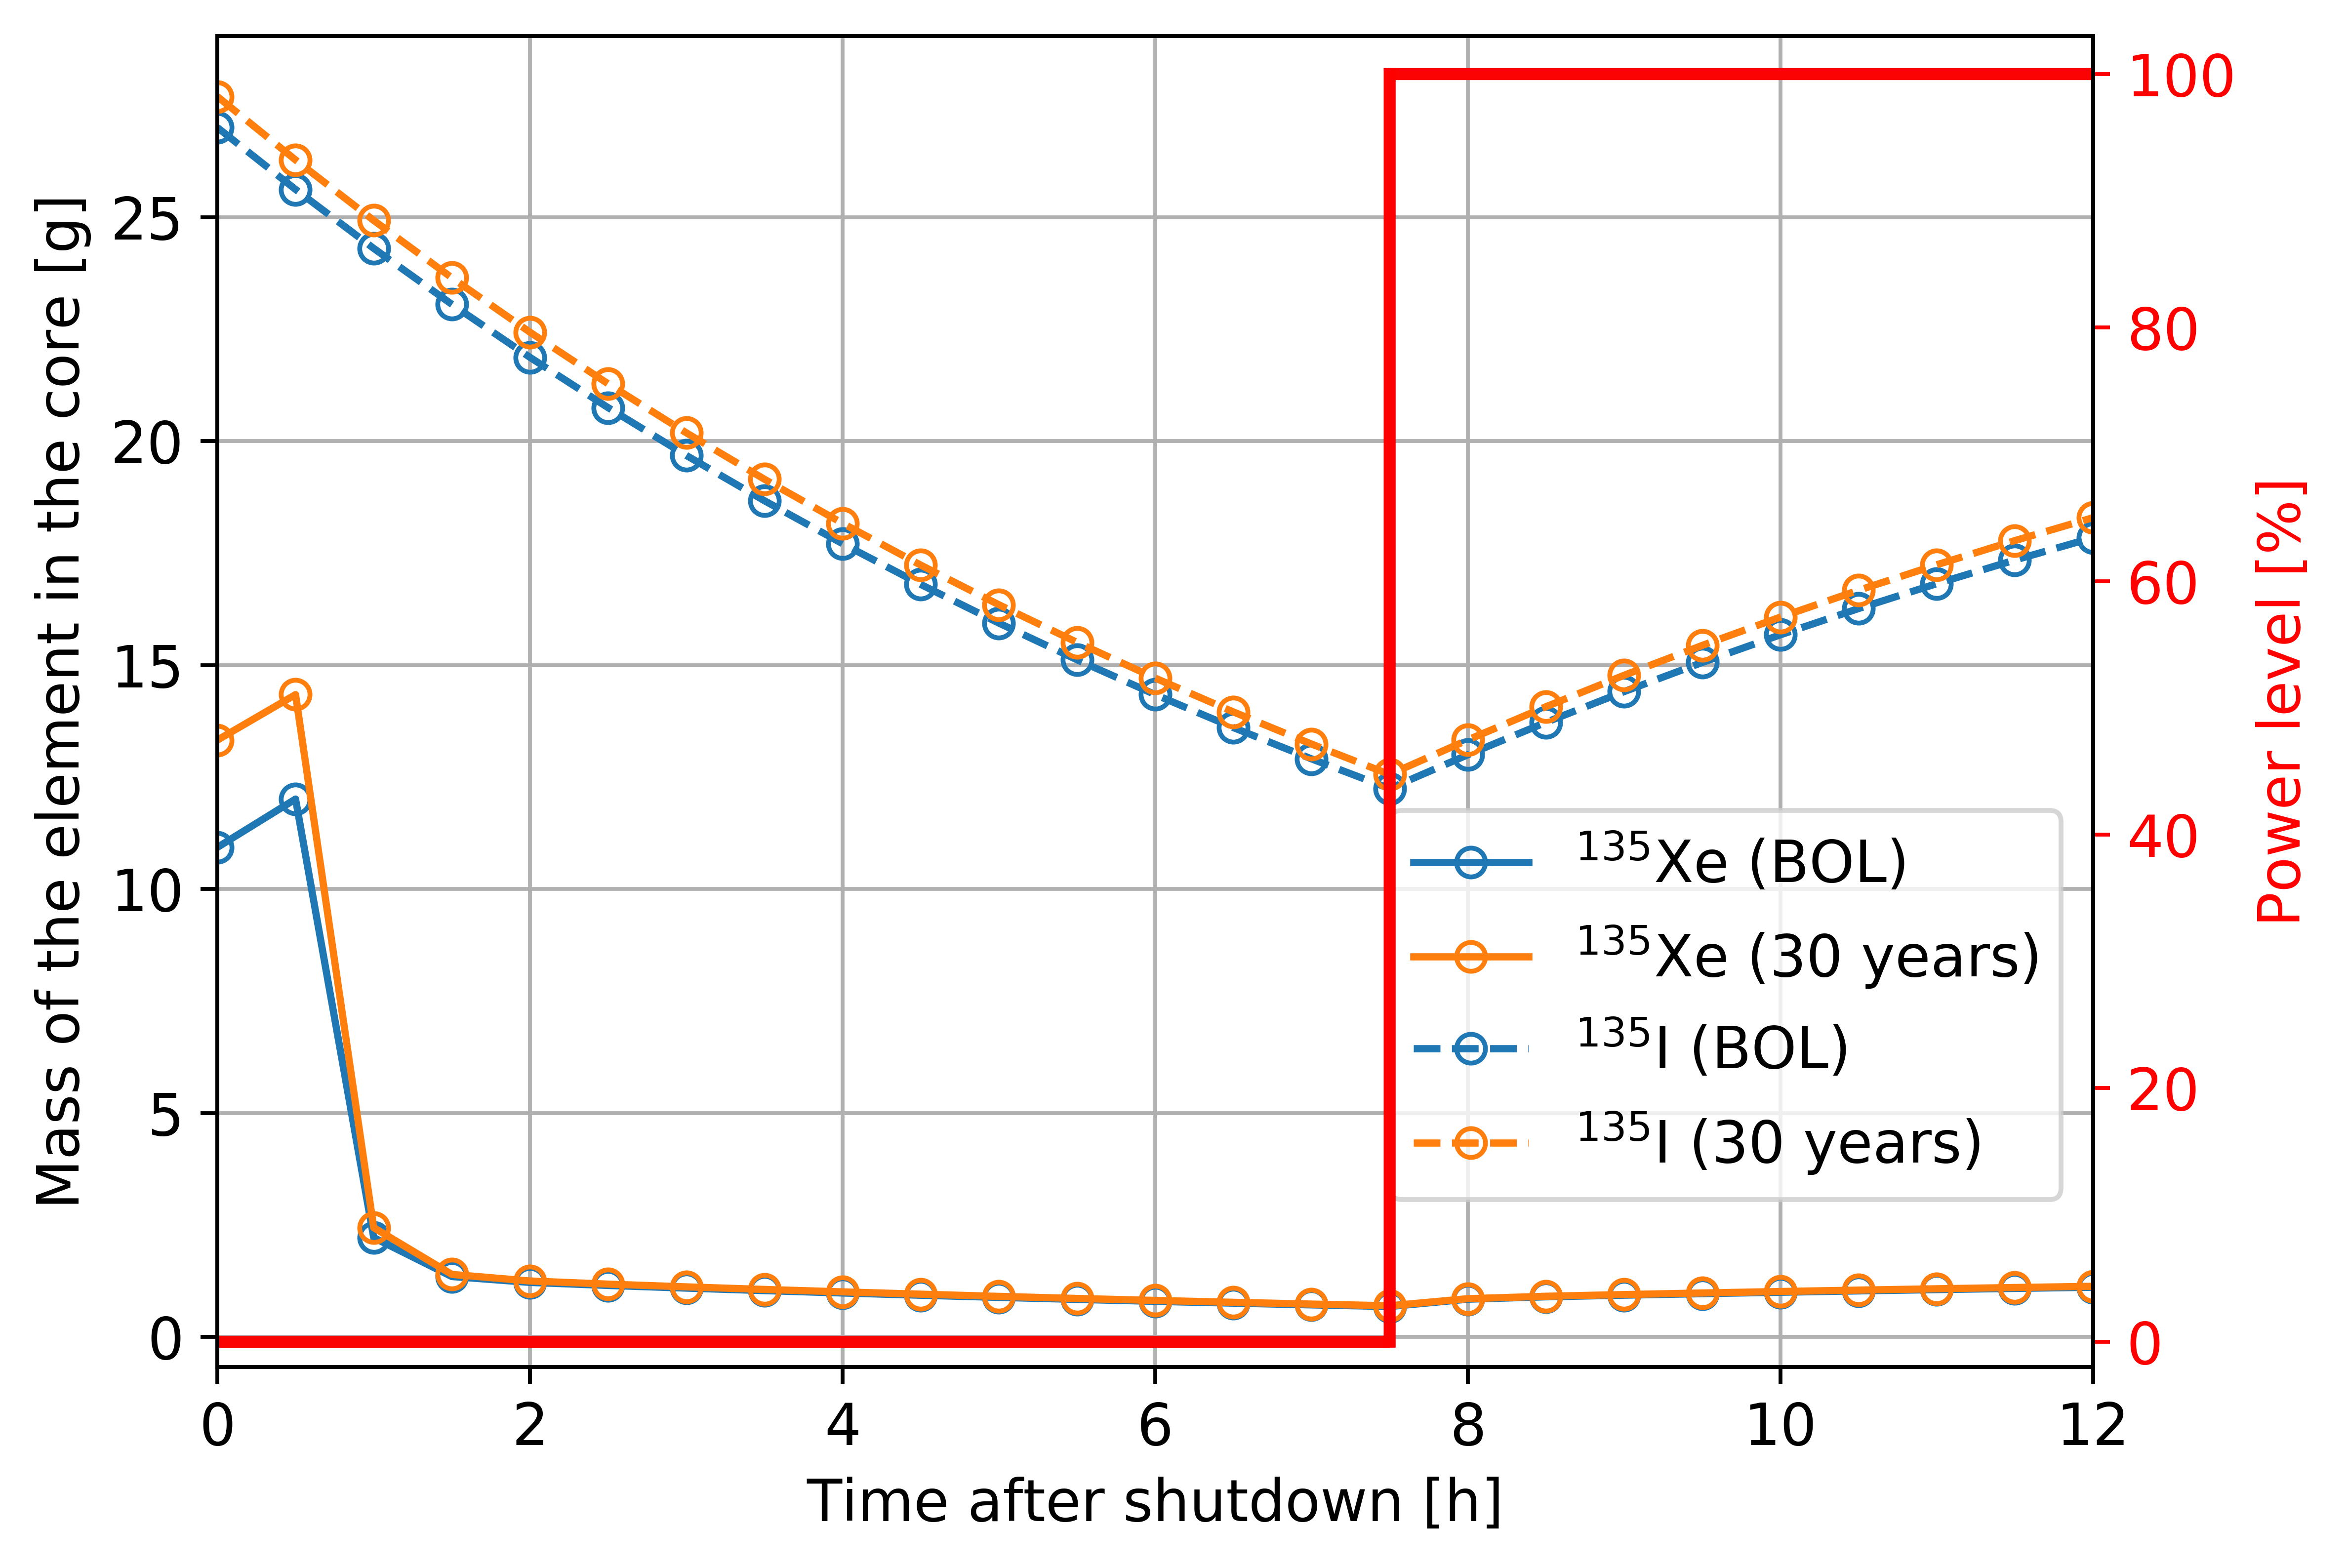
\includegraphics[width=0.88\textwidth]{ch6/kl100_xe_i_ratio.png}
	\end{array}$
	\vspace{-4mm}
	\caption{Comparison of $^{135}$Xe and $^{135}$I isotopic content at the 
		\gls{BOL} (dashed line) and after 30 years of operation (solid line) 
		for various gas removal regimes. Uncertainty of the predicted mass 
		will be estimated and discussed in Chapter 7.}
	\label{fig:msbr-lf-xe-i-ratio}
\end{figure}

Such a quick fluctuations in the $^{135}$Xe concentration are observed due to 
batch-wise nature 
of SaltProc simulations (e.g., the fraction of target poison is being 
removed discretely, at the end of each depletion step). Realistically, the gas 
removal system extracts gas from the fuel salt continuously, which would 
result in a much smoother change in the concentration and, accordingly, 
in the reactivity. Notably, for the both \gls{BOL} and \gls{EOL}, the 
$^{135}$Xe mass stabilized at 1 g in about 3-4 hours after the shutdown and 
then inclined slowly ($60$ $mg/EFPH$) after power ramp-up from 0 to 100\%. 
That is, when the reactor returned back to a full-power level,  the $^{135}$Xe 
concentration during a few days will be significantly lower than before 
load-following transient. Thus, less thermal neutrons will be parasitically 
absorbed in the fission gas. As a result, the long-term fuel cycle performance 
metrics such as fuel utilization and the core lifetime would benefit 
enormously from a ``clean-up" effect of the postulated transient, but such 
analysis is out of scope of this work.

In the case of moderate gas removal efficiency, major fission product 
concentration changes very similar to high removal efficiency case. The 
$^{135}$I/$^{135}$Xe concentration ratio is 2.15 and 2.06 at the \gls{BOL} and 
after 30 years of full-power operation, respectively, and caused 7.5\% hike 
in $^{135}$Xe concentration. Surprisingly, significantly lower gas removal 
efficiency ($\epsilon_{Xe}=0.536$ instead of 0.915) provided comparable 
benefits to the core neutronics during the postulated load-following 
transient. In fact, similarly to the $\epsilon_{Xe}=0.915$ case, the 
$^{135}$Xe mass stabilized at 1.5 g in about 5 hours after the shutdown and 
then increased slowly ($165$ $mg/EFPH$) after power ramp-up from 0 to 100\%.
In conclusion, simpler and cheaper gas removal system with extraction 
efficiency $\epsilon_{Xe}=0.536$ is good enough to suppress the xenon 
poisoning effect to acceptable level (-161 $pcm$) and ensure load-following 
capability of the \gls{MSBR}.


\subsection{Neutron spectrum}
Figure~\ref{fig:ch6-msbr-spectrum} shows that the \gls{MSBR} spectrum after 30 
years of operation (solid line) is harder than at the startup (dashed line). 
Compared with the \gls{MSBR}, the \gls{TAP} \gls{MSR} spectrum is 
significantly 
harder even when all moderator rods are inserted to the core. Notably, the 
\gls{MSBR} spectrum has clear peak in thermal energy region, but flat neutron 
energy dependence in intermediate and fast energy region, which is quite 
common for thermal reactors. In contrast, the \gls{TAP} core spectrum at the 
\gls{EOL} has high peak in fast and lower peak in thermal energy region, 
which is typical for epithermal/intermediate reactors. This is main reason, 
why for the postulated load-following transient I observed significant xenon 
poisoning effect in the \gls{MSBR} and negligible xenon impact in the 
\gls{TAP} \gls{MSR} (see Chapter 5).
\begin{figure}[htbp!] % replace 't' with 'b' to 
	\centering
	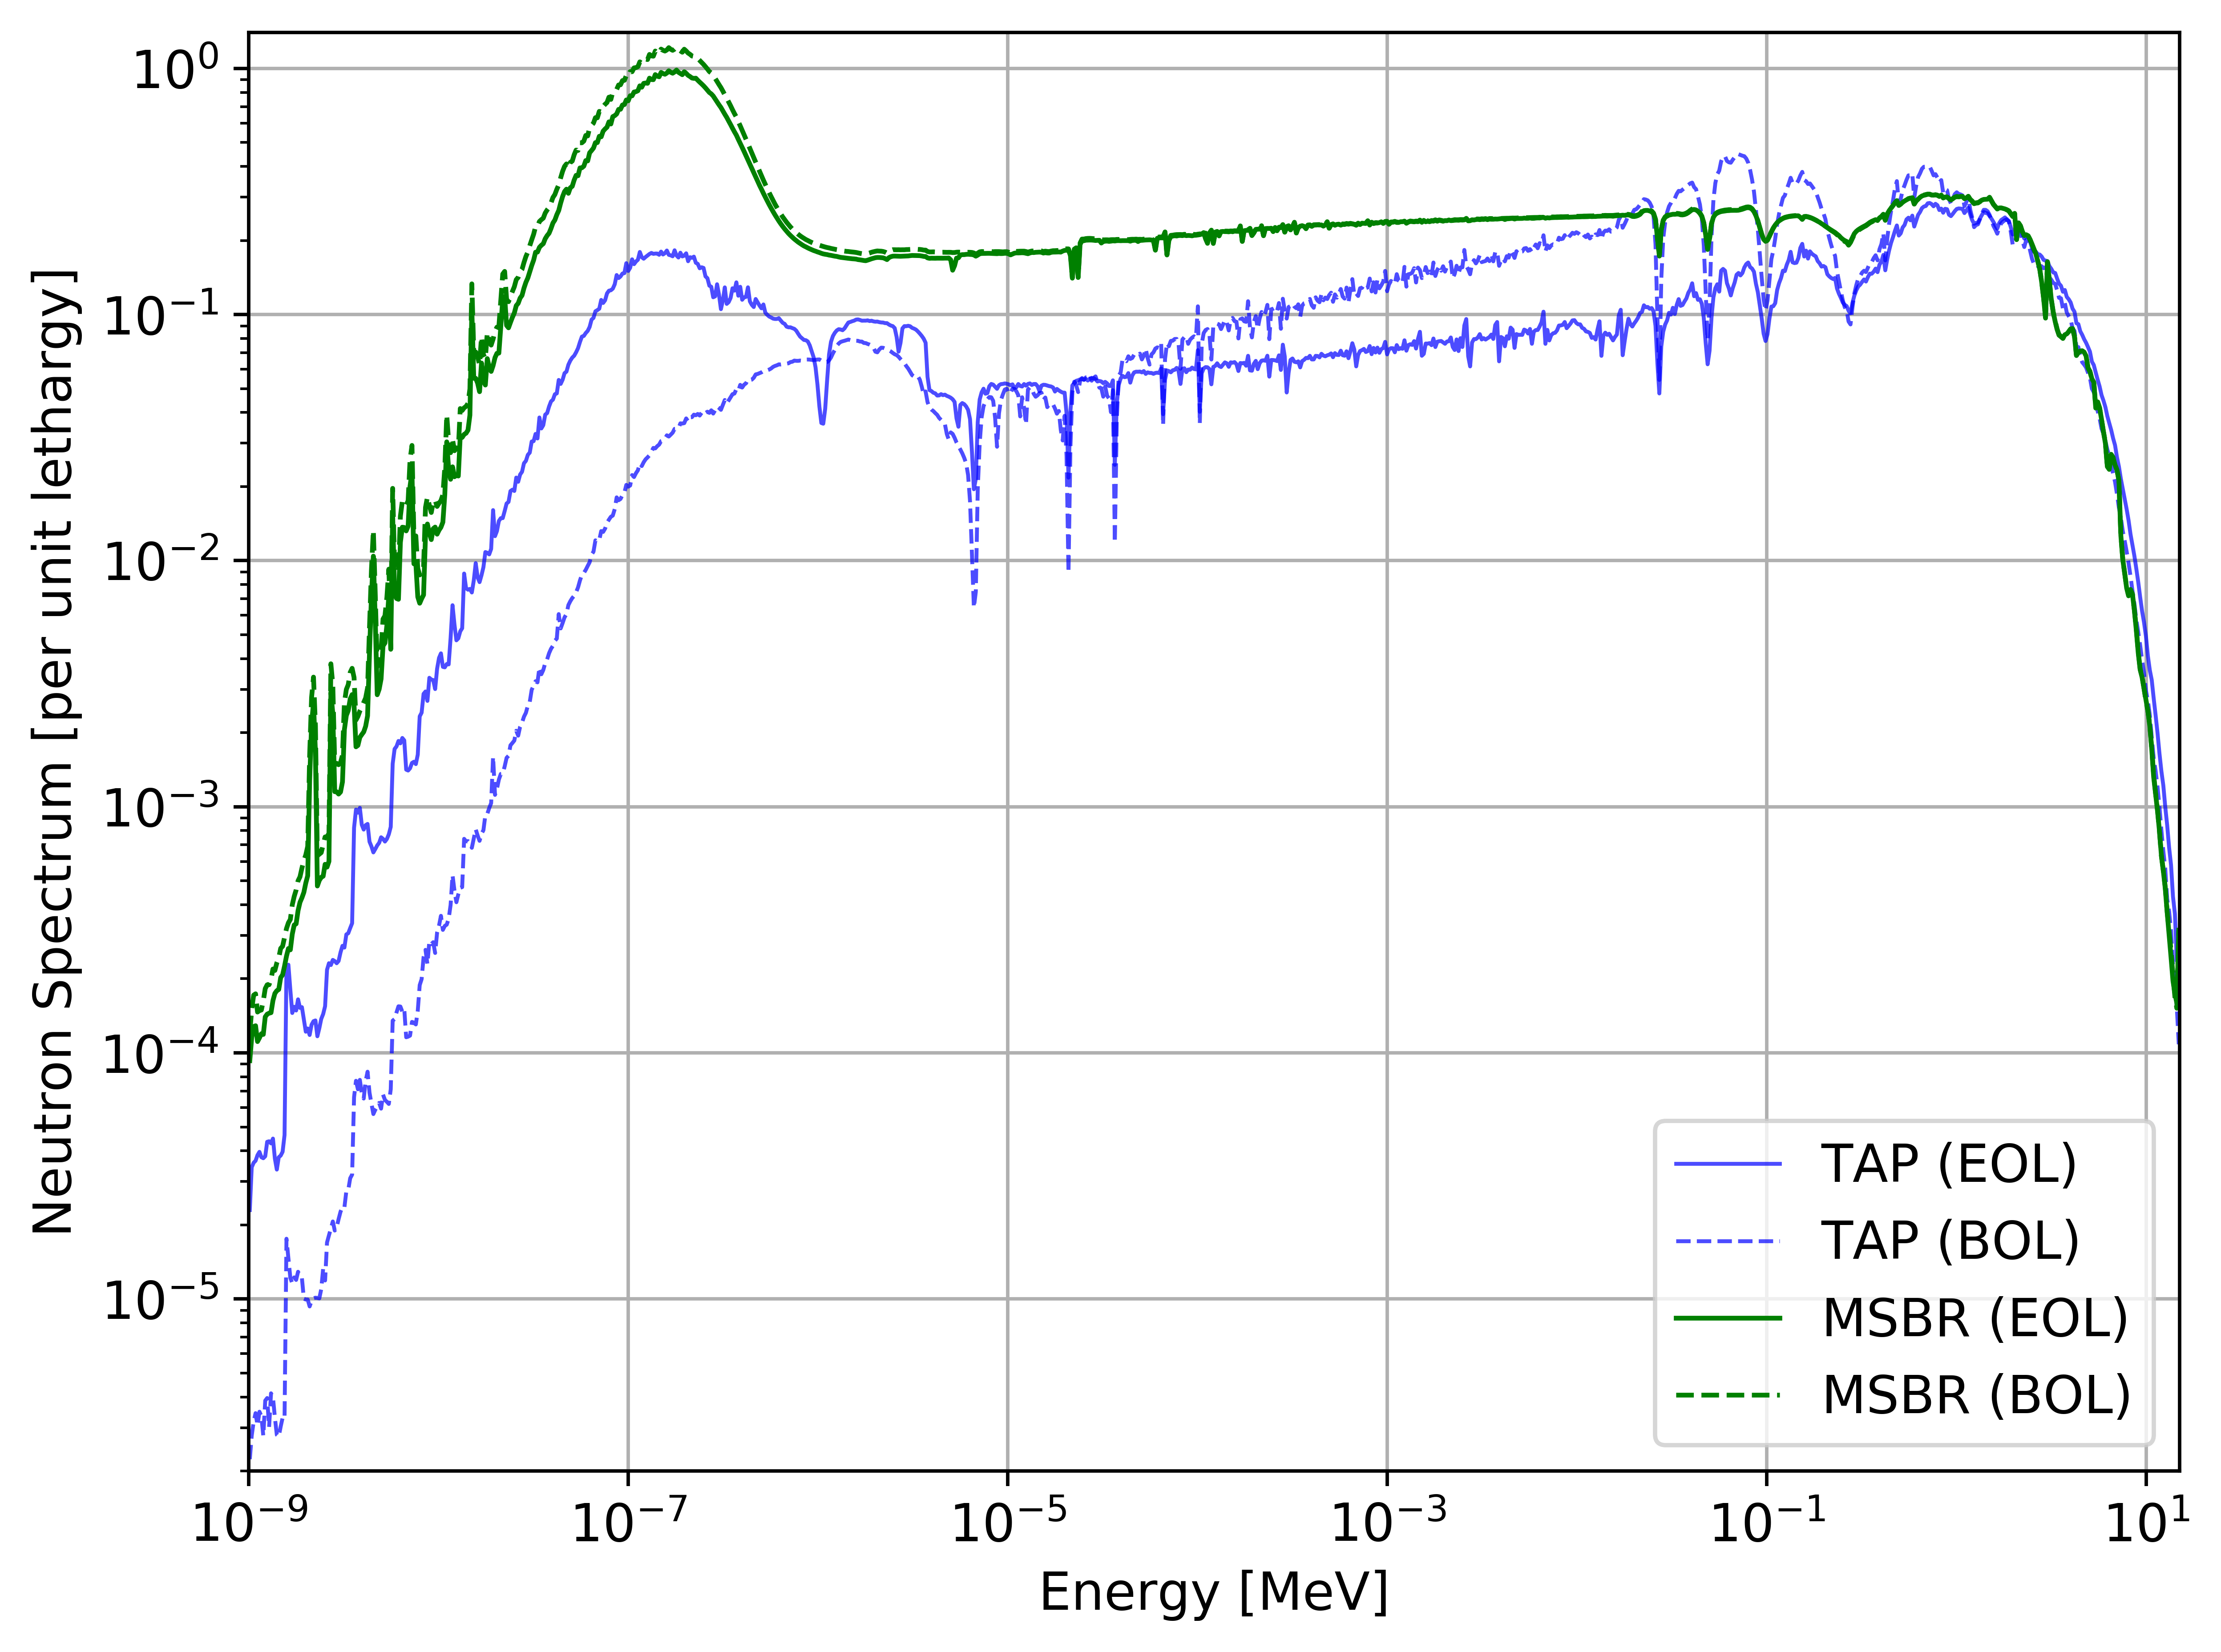
\includegraphics[width=\textwidth]{ch6/msbr_vs_tap_spectrum.png}
	\caption{Neutron spectra normalized by lethargy for the \gls{MSBR} and 
		\gls{TAP} at various moments during operation. The neutron flux 
		uncertainties $\sigma_{\Phi}$ are 0.6\% and 0.18\% for the \gls{TAP} 
		reactor and \gls{MSBR}, respectively.}
	\label{fig:ch6-msbr-spectrum}
\end{figure}

Potentially, any graphite-moderated liquid-fueled \gls{MSR} conceptual 
design\footnote{Integral Molten Salt Reactor (IMSR) from Terrestial Energy 
\cite{leblanc_integral_nodate}, Molten Salt Demonstration Reactor (MSDR) from 
Oak Ridge National Laboratory \cite{bettis_design_1972}, Liquid fluoride 
thorium reactor (LFTR) from Flibe energy \cite{sorensen_liquid-fluoride_2016}, 
etc.} would demonstrate similar benefits from the presents of the online gas 
removal system within nuclear island.


\section{Safety and operational parameters}
The significant changes of strong absorbers concentration in the fuel slightly 
shift the core spectrum which potentially might impact the reactor safety.
Rapid changes in fuel salt composition should not compromise critical safety 
margins.
I calculated major safety and operational parameters at various moments 
throughout the postulated transient using approaches from 
Sections~\ref{sec:safety-param} and \ref{ch5:saf_param}. 
The total temperature coefficient of reactivity ($\alpha_{ISO}$) must remain 
negative and the total control rod worth (CRW) must be sufficient to trip the 
reactor throughout the postulated transient. Ideally, we want to major safety 
and operational parameters stay almost constant because the changes in those 
parameter would require fast response from reactor control systems (i.e., the 
control rod jerk in response to the CRW change).

\subsection{Temperature coefficient of reactivity}
Figure~\ref{fig:msbr-lf-tc-evo} shows the temperature feedback coefficient 
dynamics for the \gls{MSBR} during the transient for various gas removal 
efficiencies ($\epsilon_{Xe}=0.536$ and 0.915). 
The Fuel Temperature Coefficient ($\alpha_{T,F}$) becomes less negative at the 
beginning of the transient for all cases. The reason for this is a 
slight spectrum hardening due to the $^{135}$Xe concentration peak changed the 
Doppler broadening of resonances. After that, the magnitude of $\alpha_{T,F}$ 
slowly inclined due to $^{135}$Xe removal from the fuel.
\begin{figure}[htbp!] % replace 't' with 'b' to 
	\centering
	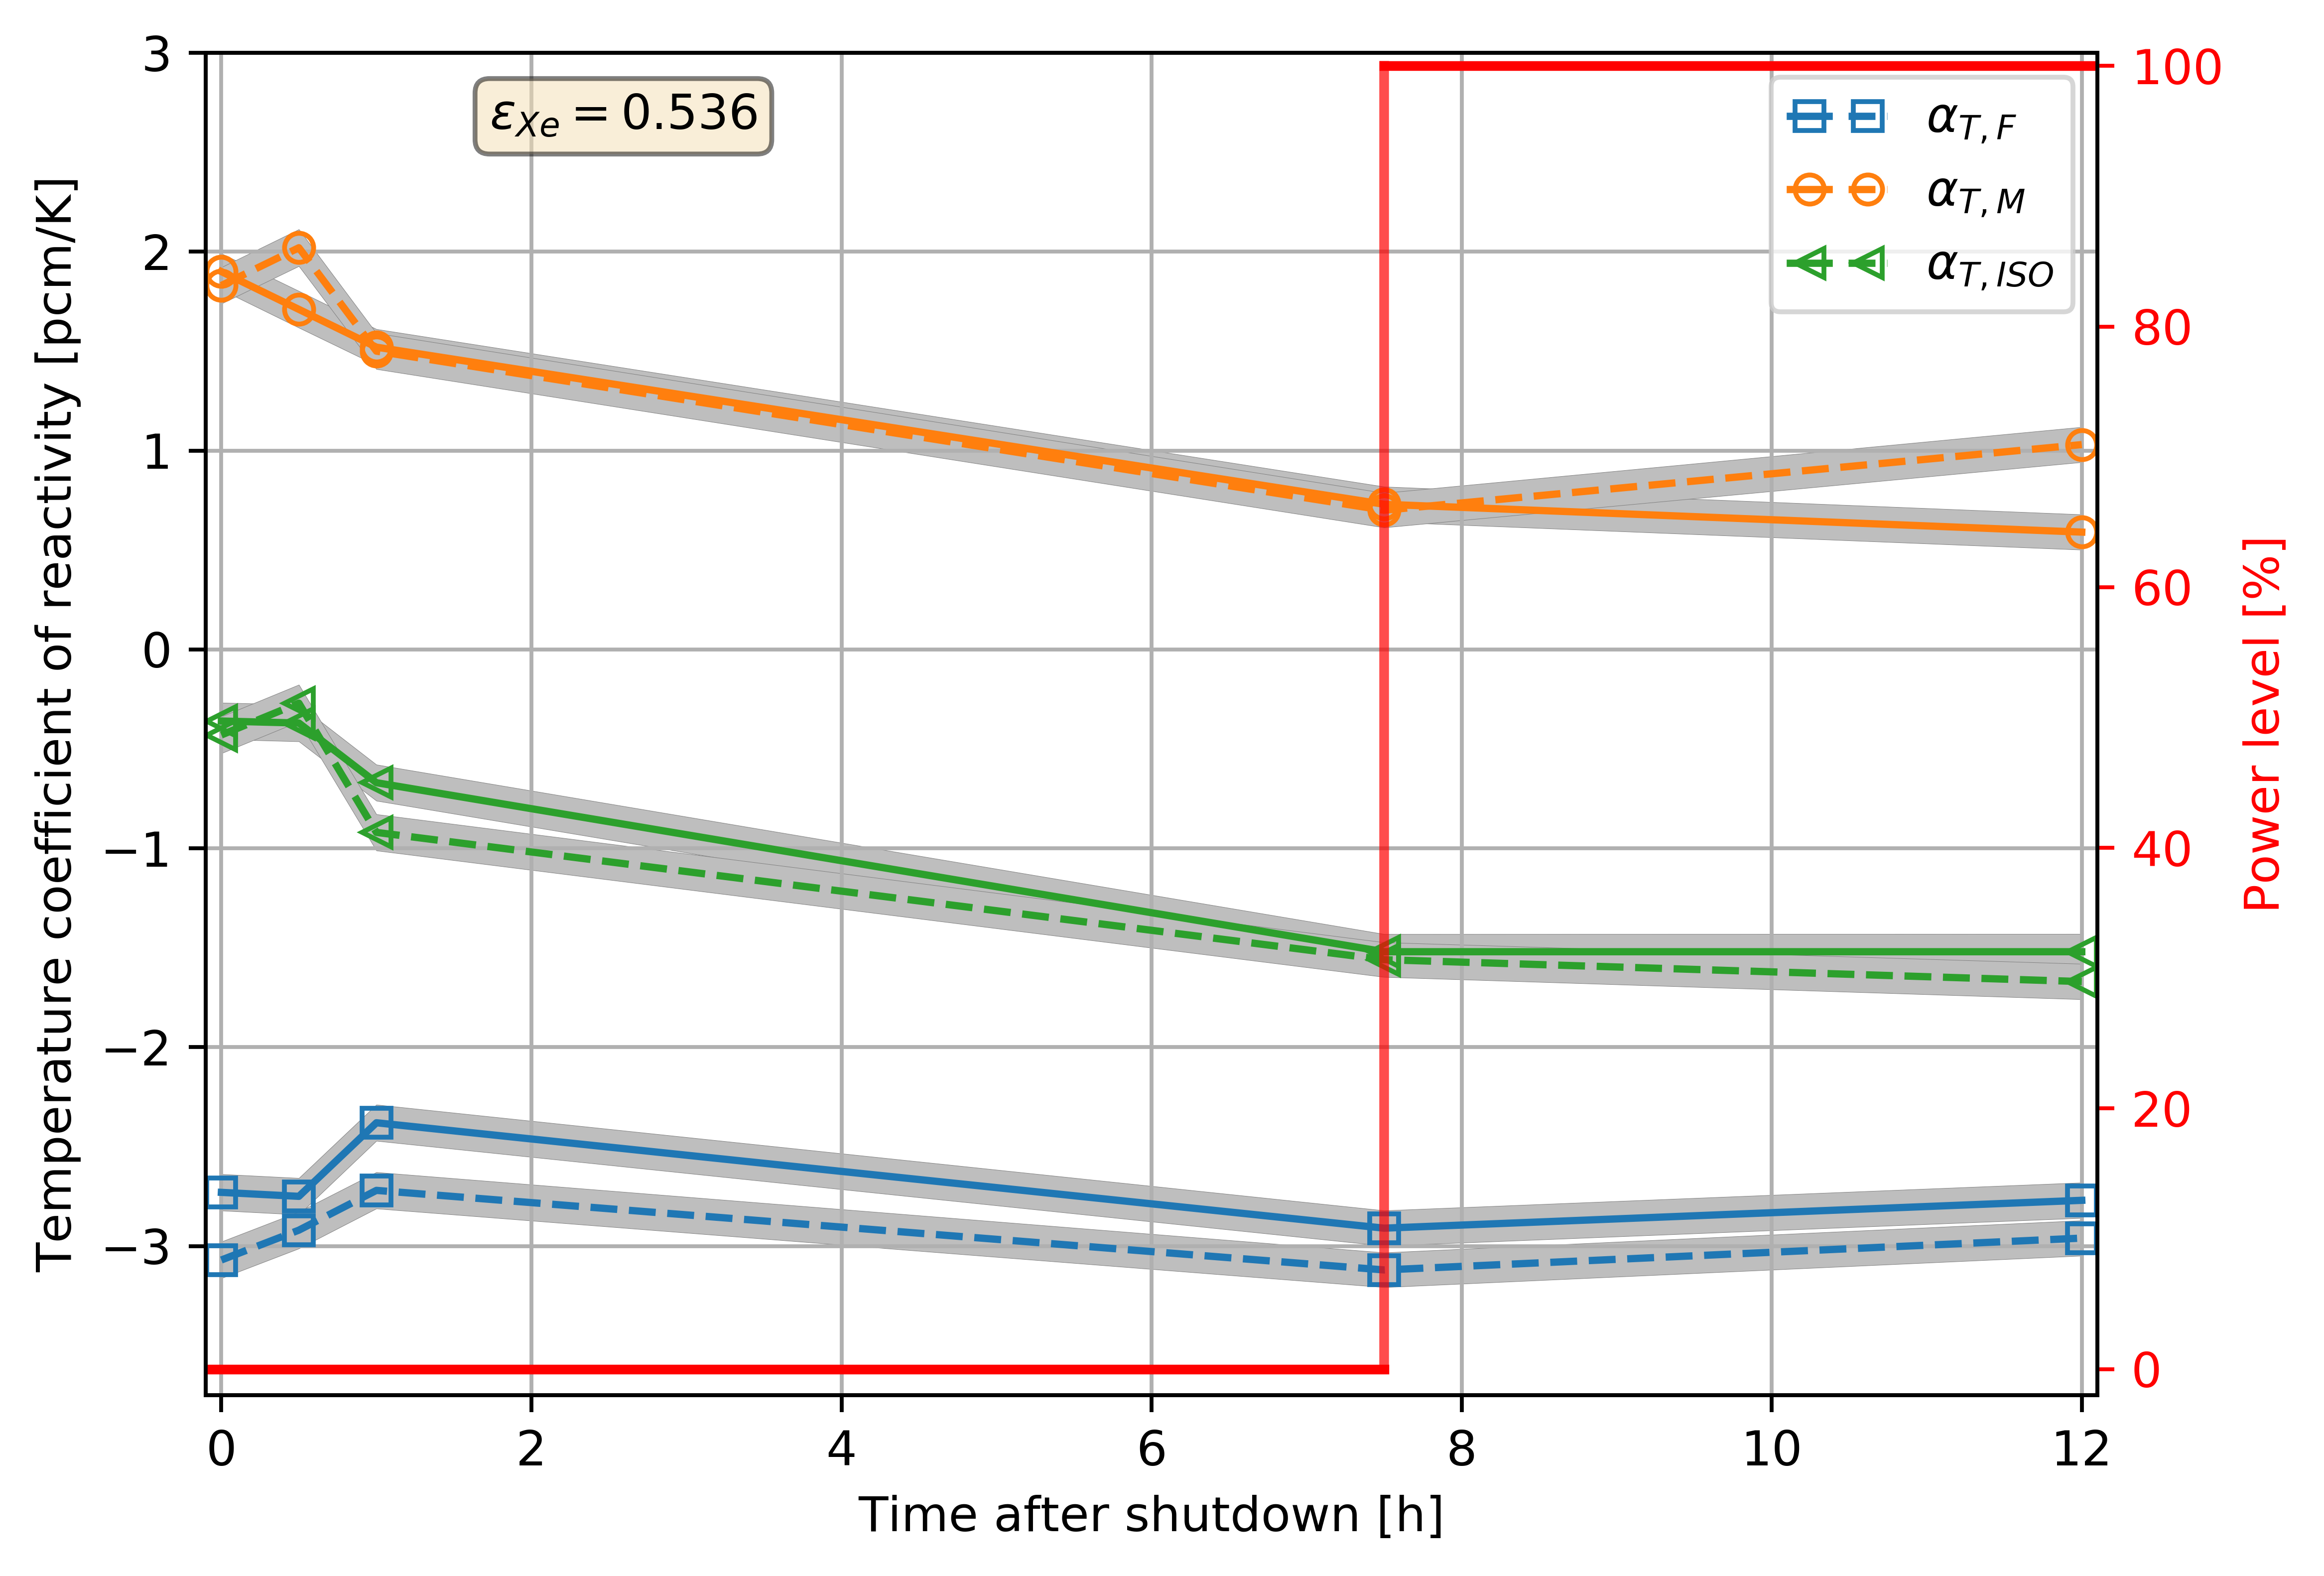
\includegraphics[width=0.95\textwidth]{ch6/saf_par/tc_evo_kl25.png}\\
	\vspace{-12mm}
	\hspace{+0.05mm}
	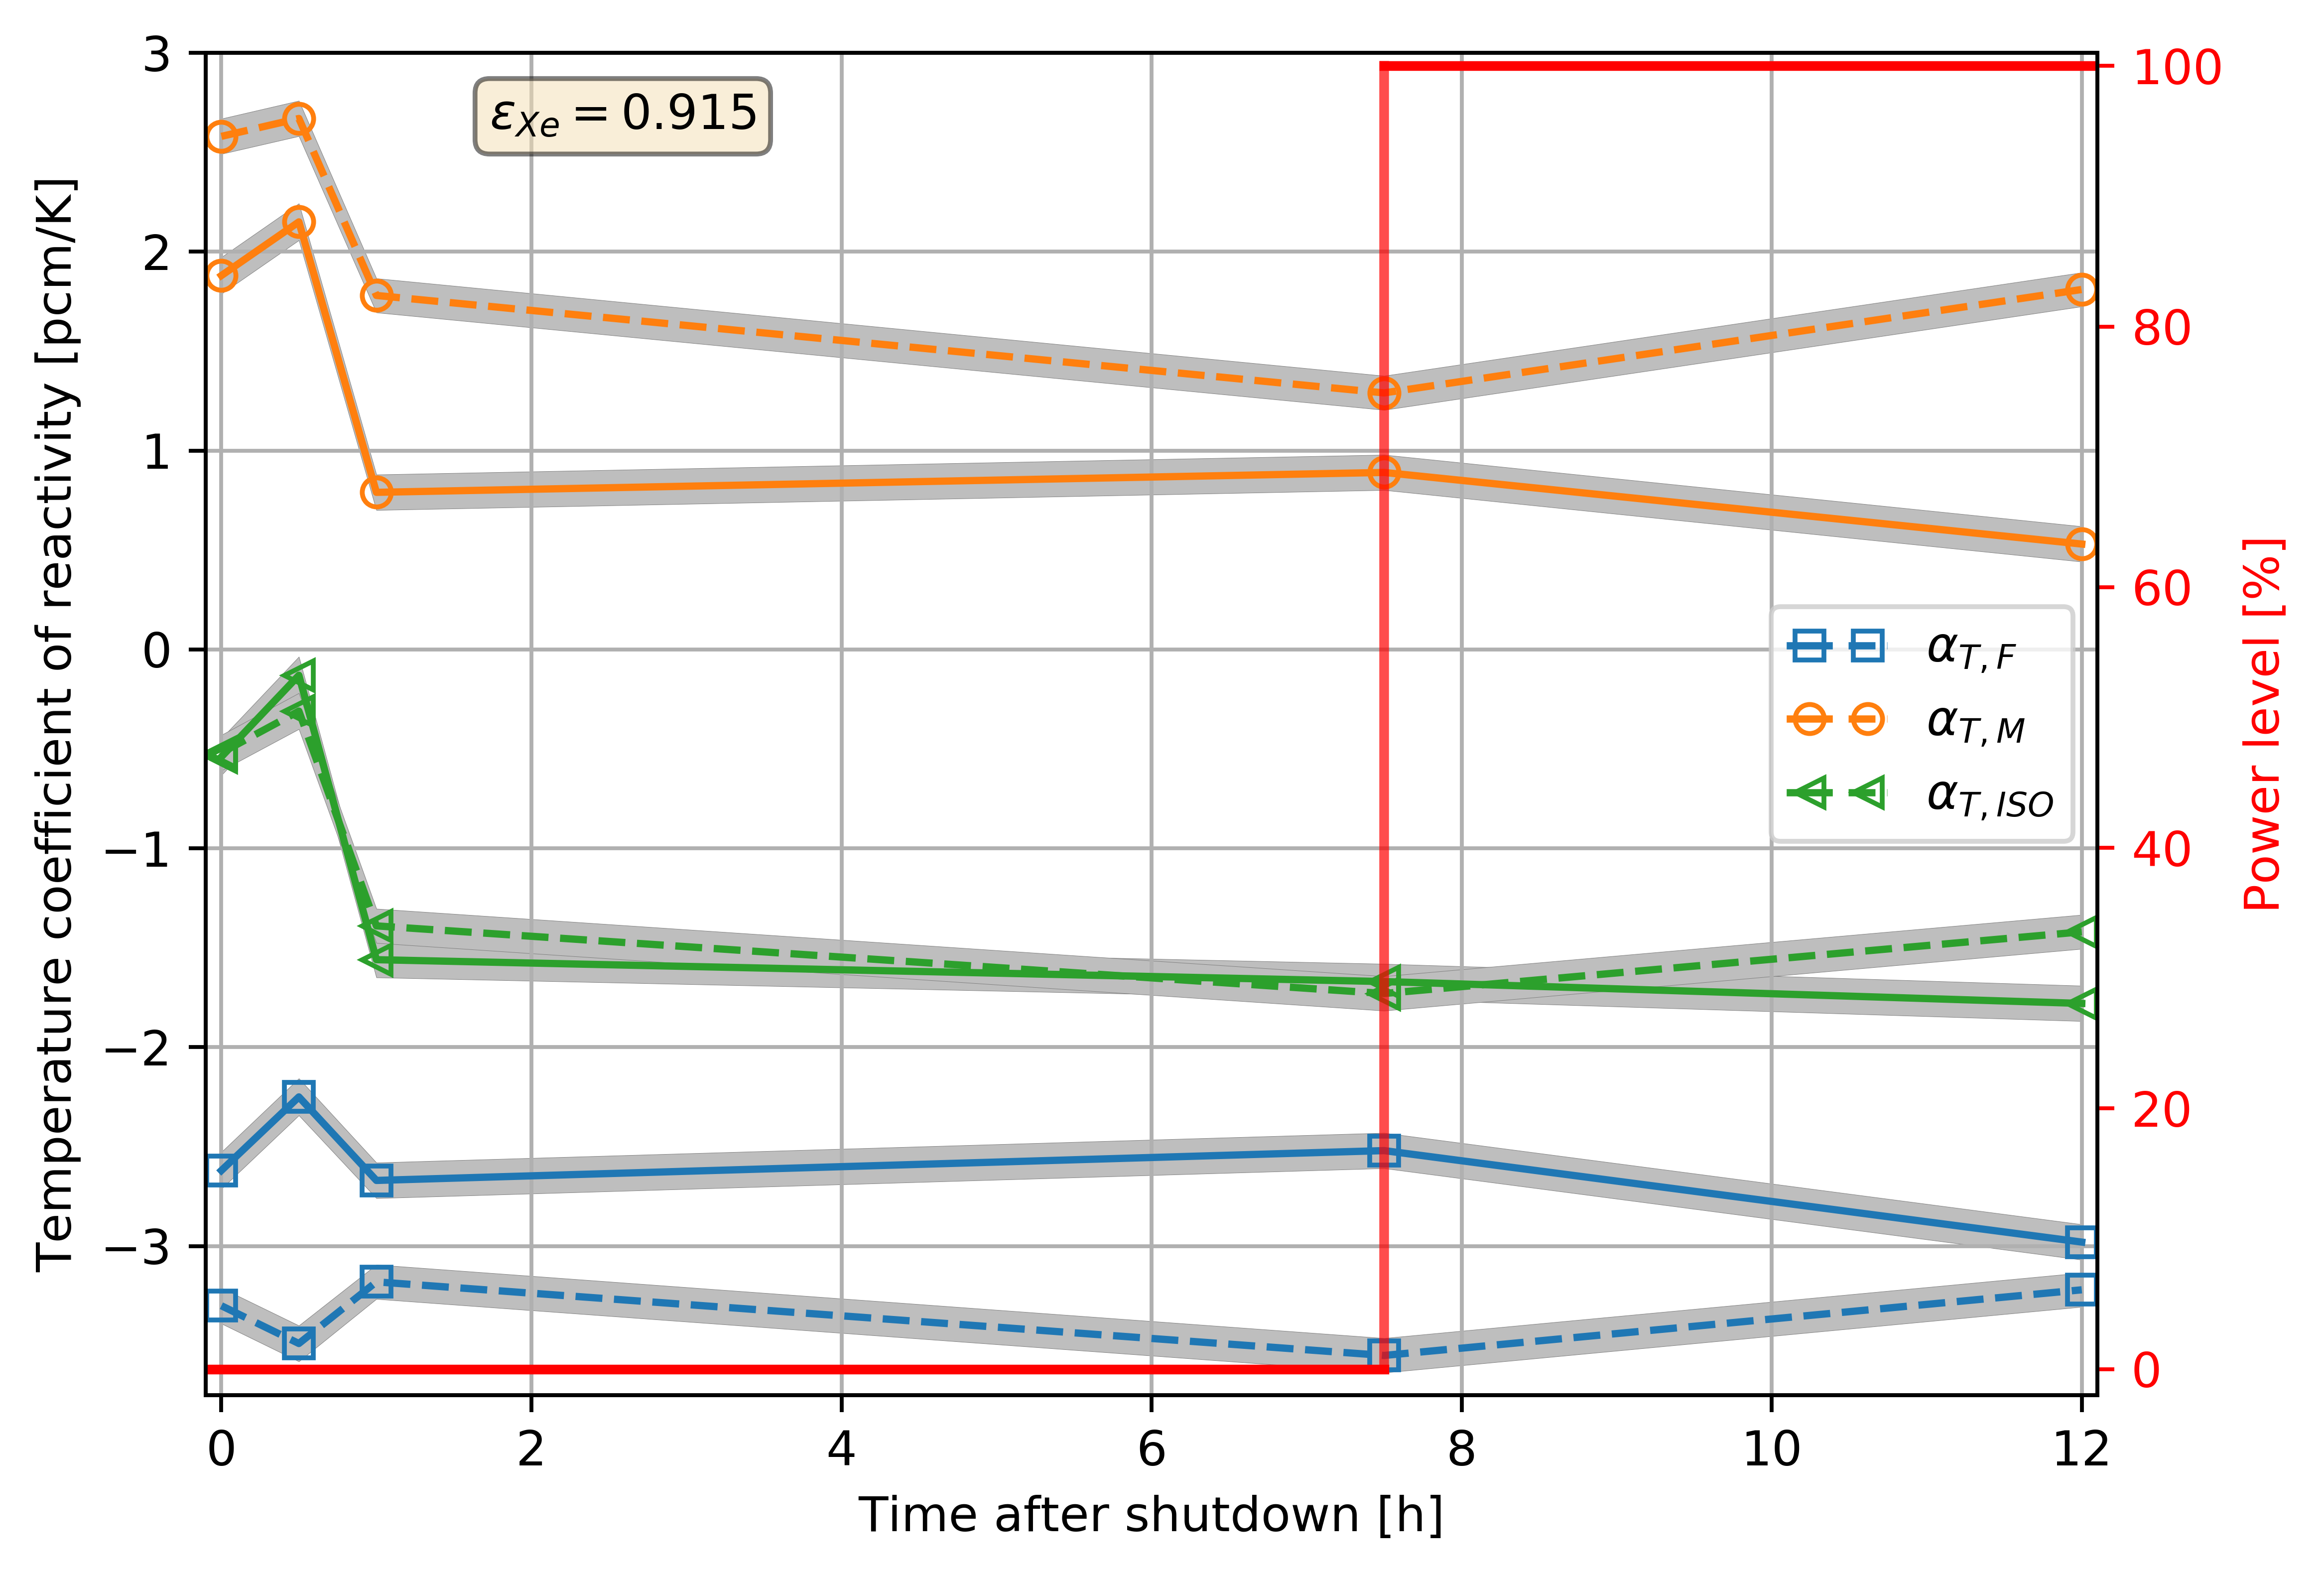
\includegraphics[width=0.95\textwidth]{ch6/saf_par/tc_evo_kl100.png}
	\vspace{-3mm}
	\caption{Temperature feedback coefficients during the postulated transient 
	for the \gls{MSBR} operating with moderate ($\epsilon_{Xe}=0.536$, upper) 
	and high ($\epsilon_{Xe}=0.915$, lower) gas removal efficiency at the 
	\gls{BOL} (dashed line) and after 30 years of operation (solid line).
	The	uncertainty $\pm\sigma$ is shaded.}
	\label{fig:msbr-lf-tc-evo}
\end{figure}

The isothermal temperature coefficient, $\alpha_{ISO}$, is $-0.36\pm0.09$ 
$pcm/K$ at the beginning and remains stable during first 30 minutes of the 
transient for the moderate removal efficiency case.  Then, as the gas removal 
system reduces $^{135}$Xe concentration in the core, $\alpha_{ISO}$ becomes 
even more negative: $-1.52\pm0.09$ $pcm/K$ when the $^{135}$Xe mass stabilized 
at 1.5 g in about 5 hours after the shutdown. After power ramp-up from 0\% to 
100\%, $\alpha_{ISO}$ remains stable since the $^{135}$Xe mass increasing very 
slowly. On the whole, another interesting benefit from the online gas removal 
is improved passive safety (stronger temperature feedback coefficient) 
throughout and, possibly, a few days after the postulated transient due to low 
concentration of the $^{135}$Xe in the fuel salt.

For the high gas removal efficiency regime ($\epsilon_{Xe}=0.915$), the 
isothermal temperature coefficient worsens from $-0.54\pm0.09$ $pcm/K$ to 
approximately $-0.22\pm0.09$ $pcm/K$ during first 30 minutes after shutdown. 
Afterwards, when the gas removal system extracted major fraction of the 
$^{135}$Xe from the fuel salt, $\alpha_{ISO}$ became significantly more 
negative ($-1.39$ and $-1.56$ $pcm/K$ at the \gls{BOL} and after 30 years of 
operation, respectively) due to the spectrum softening. In brief, the 
temperature feedback in the \gls{MSBR} becomes stronger when neutron poisons 
concentration in the fuel decreases. As a result, flattening the $^{135}$Xe 
concentration peak improves the \gls{MSBR} passive safety.

Overall, the combination of fuel and moderator thermal feedback coefficients, 
$\alpha_{ISO}$, remains negative throughout the postulated transient. 
Moreover, simpler and cheaper gas removal system with extraction 
efficiency $\epsilon_{Xe}=0.536$ provided more predictable thermal feedback 
coefficient dynamics throughout the transient due to 
a more gradual change in the $^{135}$Xe concentration.

\subsection{Void coefficient of reactivity}
Figure~\ref{fig:msbr-lf-void-evo} demonstrates the void coefficient of 
reactivity evolution during the postulated transient. 
In contrast with the \gls{TAP} \gls{MSR}, the void coefficient of reactivity 
after 30 years of full-power operation is substantially greater than at the 
startup for both gas removal regimes. The reason for this is the \gls{MSBR} 
spectrum hardening toward \gls{EOL}, which is opposite to the \gls{TAP} 
\gls{MSR} spectrum evolution. Thus, an unexpected void insertion due to the 
gas separation system failure would lead to more severe consequences toward 
\gls{EOL}. 
\begin{figure}[htbp!] % replace 't' with 'b' to 
	\centering
	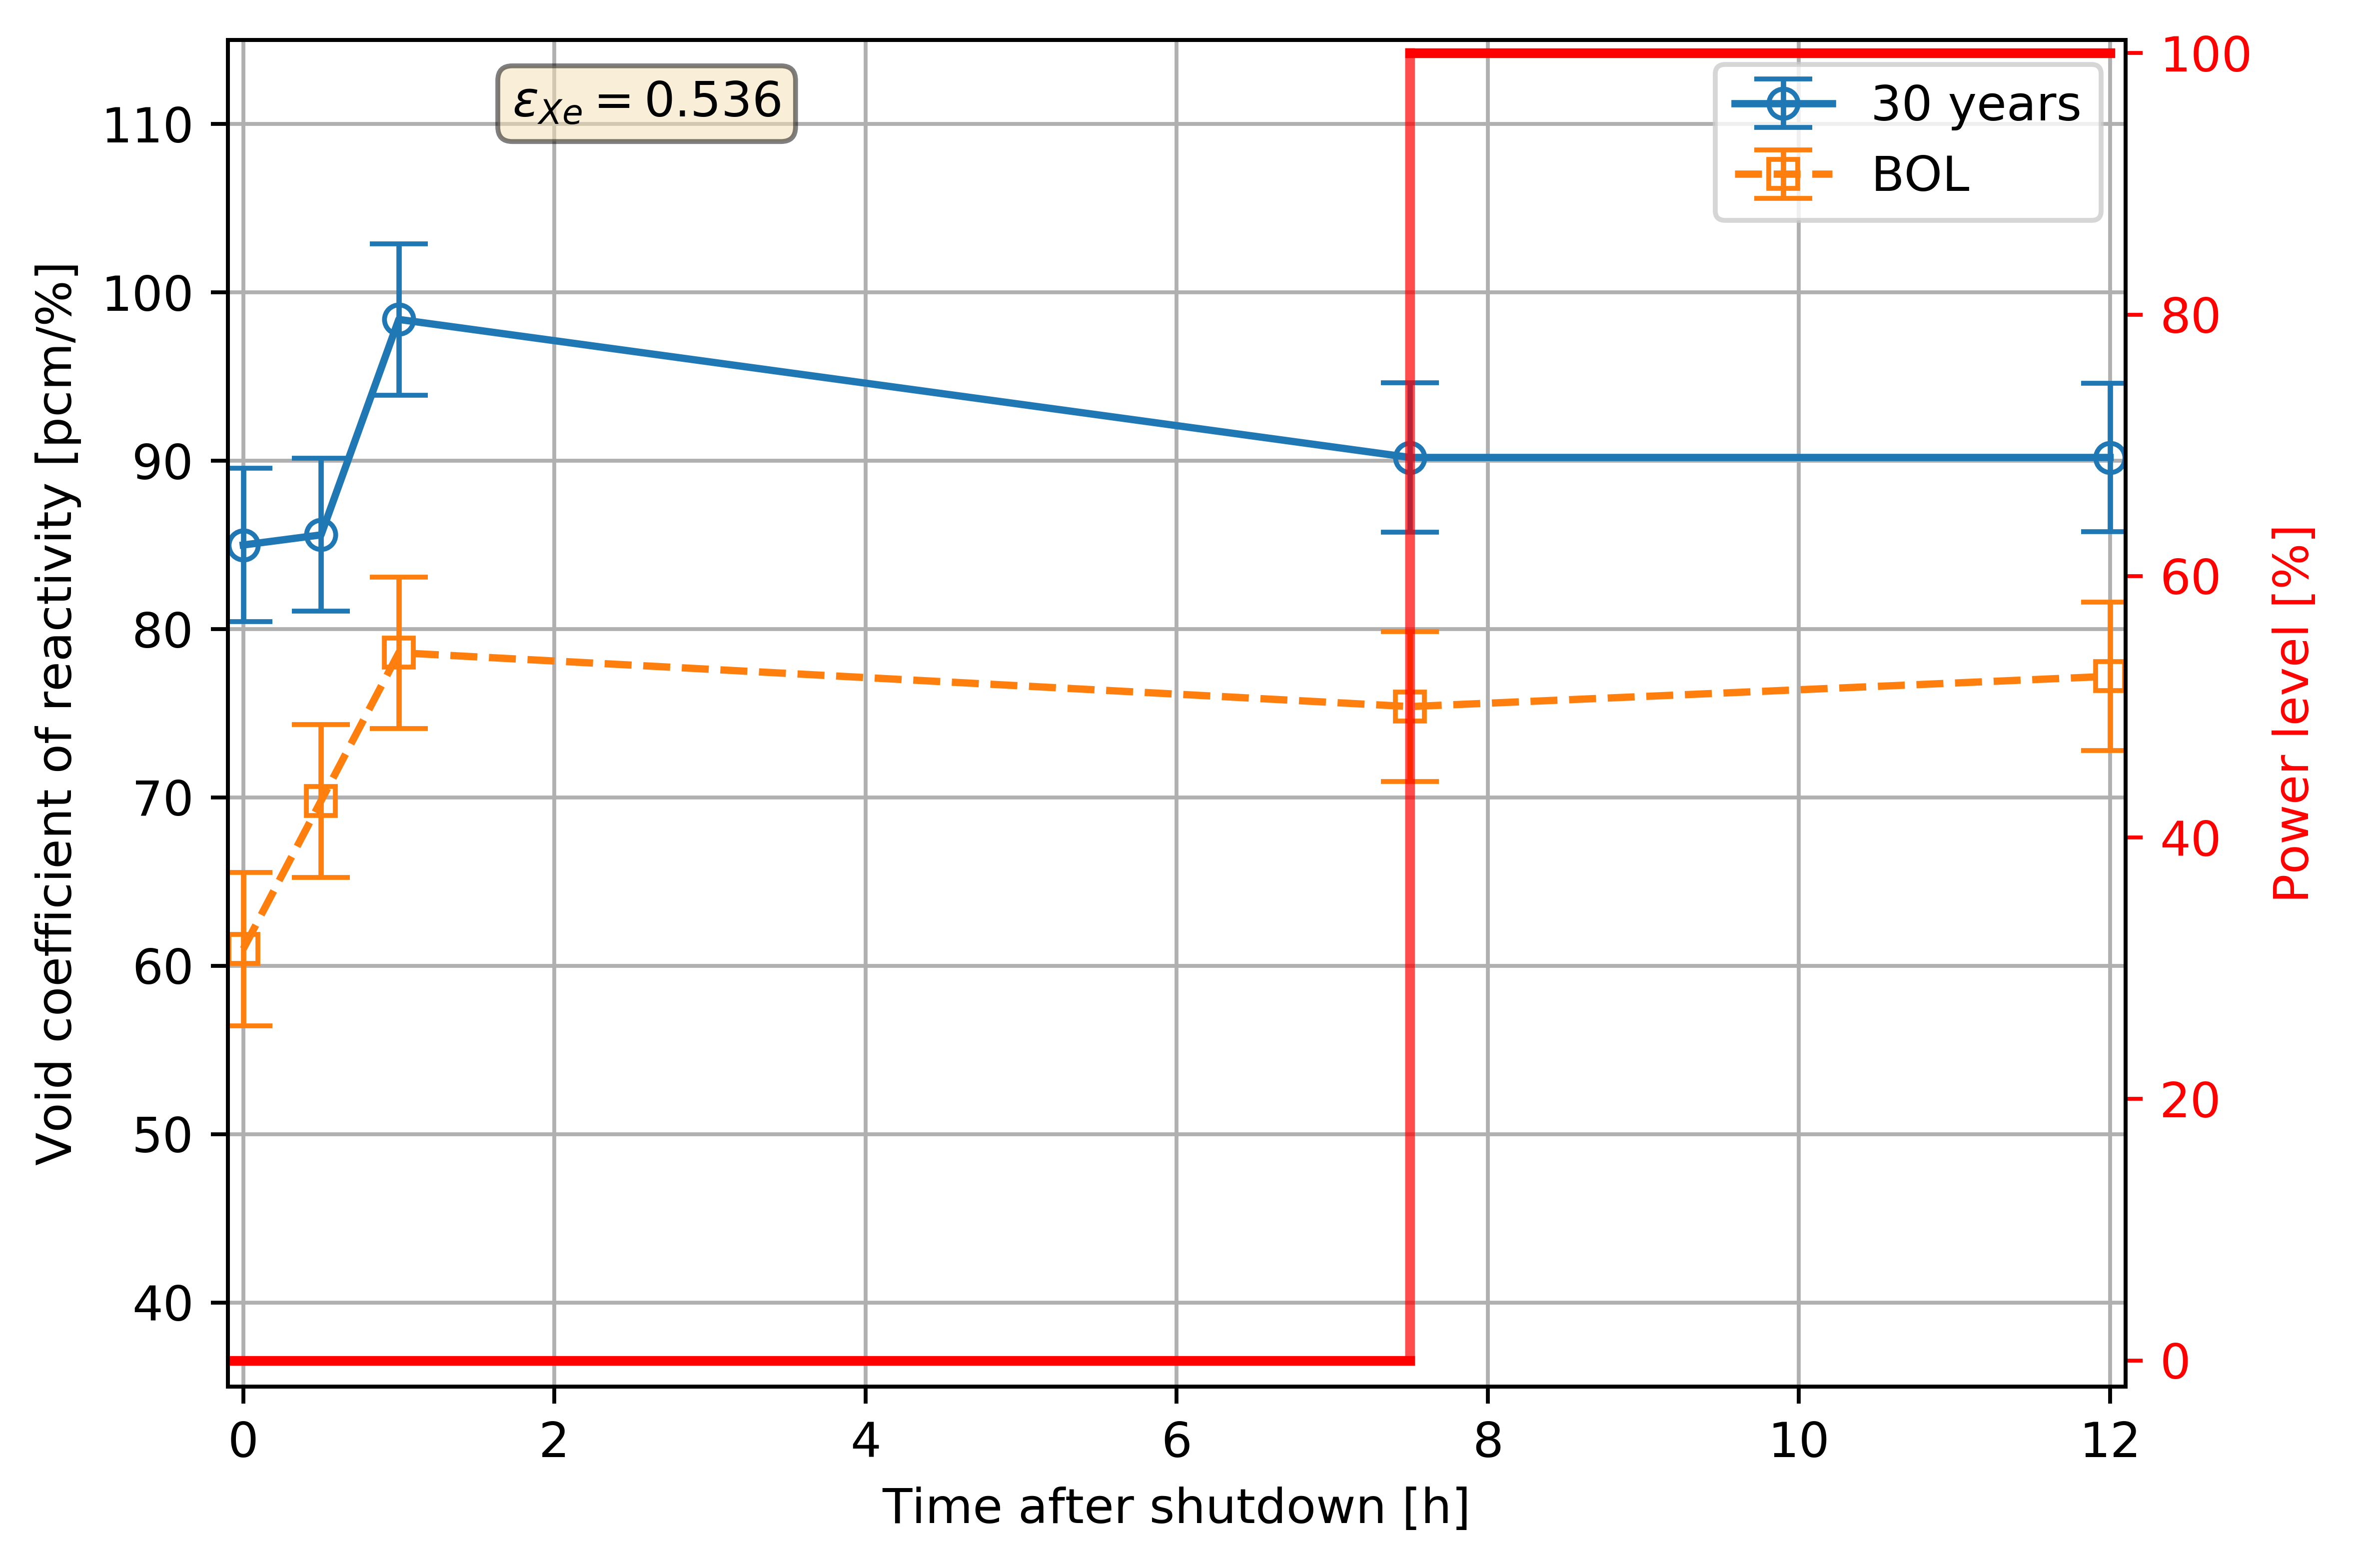
\includegraphics[width=0.92\textwidth]{ch6/saf_par/void_evo_kl25.png}\\
	\vspace{-12mm}
	\hspace{+0.05mm}
	\includegraphics[width=0.92\textwidth]{ch6/saf_par/void_evo_kl100.png}
	\vspace{-3mm}
	\caption{Void coefficient of reactivity as a function of time during 
	postulated transient
for the \gls{MSBR} operating with moderate 
	($\epsilon_{Xe}=0.536$, upper) and high ($\epsilon_{Xe}=0.915$, lower) gas 
	removal efficiency at the \gls{BOL} (dashed line) and after 30 years of 
	operation (solid line).}
	\label{fig:msbr-lf-void-evo}
\end{figure}

For the high gas removal efficiency, $\alpha_V$ fluctuates during the 
postulated transient between 42 and 61 $pcm/$void\% at the \gls{BOL} and 
between 87 and 102 $pcm/$void\% after 30 years of operation. The $^{135}$Xe 
concentration spike caused corresponding $\alpha_V$ drop due to short-term 
spectrum hardening. Then, $\alpha_V$ quickly recovers to its initial value. 
Similarly to the temperature feedback coefficient, the moderate gas removal 
efficiency provided more predictable $\alpha_V$ dynamics throughout the 
transient. Additionally, significantly smaller $\alpha_V$ raise toward 
\gls{EOL} for the case with $\epsilon_{Xe}=0.536$ ($\Delta\alpha_V\approx25$ 
$pcm/$void\%) will simplify the gas removal backup safety mechanism. 
Overall, all observed changes in the void coefficient of reactivity throughout 
the load-following transient for all cases are within 3-$\sigma$ range 
($\sigma_{\alpha_V}\pm5$ $pcm/$\%). This observations should be taken 
into account in the \gls{MSBR} accident analysis and safety
justification.

\subsection{Reactivity control rod worth}
Figure~\ref{fig:lf-msbr-crw-evo} shows the control rod worth evolution 
during the postulated transient. For the high gas removal efficiency regime 
with the \gls{EOL} fuel composition, the control rod worth dropped by $46\pm9$ 
$pcm$ during first 30 minutes after the shutdown due to short-term spectrum 
hardening related to the $^{135}$Xe concentration peak. In next 30 minutes, 
the CRW recovers to its initial value and keeps increasing throughout the 
transient because the gas removal system steadily reduces $^{135}$Xe 
concentration in the core. Notably, the control rod worth is greater at the 
\gls{BOL} because the $^{10}$B (used as absorber in the control rods) 
absorption cross section declines rapidly with energy. Overall, the control 
rod worth benefits from the \gls{MSBR} spectrum softening toward \gls{EOL}.

For the moderate gas separation efficiency regime, the control rod worth 
remains almost constant during first hour after shutdown for the both 
\gls{BOL} and \gls{EOL}. Afterwards, the CRW increased by 4\% due to the 
spectrum softening caused by the $^{135}$Xe concentration incline. As for 
other safety parameters, the control rod worth also benefits 
from less effective gas removal system due to smother xenon concentration 
dynamics, and, thus, more predictable neutron spectrum shift. 
\begin{figure}[htbp!] % replace 't' with 'b' to 
	\centering
	\includegraphics[width=0.95\textwidth]{ch6/saf_par/crw_evo_kl25.png}\\
	\vspace{-10mm}
	\hspace{+0.05mm}
	\includegraphics[width=0.95\textwidth]{ch6/saf_par/crw_evo_kl100.png}
	\vspace{-3mm}
	\caption{Total control rod worth as a function of time during 
		postulated transient
for the \gls{MSBR} operating with moderate 
		($\epsilon_{Xe}=0.536$, upper) and high ($\epsilon_{Xe}=0.915$, lower) 
		gas removal efficiency at the \gls{BOL} (dashed line) and after 30 
		years of operation (solid line).}
	\label{fig:msbr-lf-crw-evo}
\end{figure}

Unfortunately, the total control rod worth is insufficient to shut down the 
reactor throughout the postulated transient. The reactivity change during the 
transient is up to 2550 $pcm$ while the total control rod worth is only about 
$1250-1425$ $pcm$. The \gls{MSBR} was designed with only two graphite and two 
boron-carbide rods located in the center of the core (see 
Figure~\ref{fig:msbr_elev_view}) for operative reactivity control and relied 
heavily on fissile feed adjustment as a primary reactivity control 
mechanism. However, the fissile feed cannot be adjusted quickly and nuclear  
regulations required control rods have sufficient worth to safely shut down 
the reactor at any time. Therefore, the control rods design in the \gls{MSBR} 
must be reexamined to ensure the total control rod worth at least 3000 $pcm$ 
to ensure safety during the transient with rapid power change.


\section{Concluding remarks}
This chapter demonstrated SaltProc v1.0 capabilities to simulate the 
short-term depletion with the power variation from 0\% to 100\% for the 
\gls{MSBR}. I applied methodology from Chapter 5 to investigate the xenon 
poisoning effect in the \gls{MSBR} for three various gas removal system 
regimes: (1) no gas removal ($\epsilon_{Xe}=0.0$), (2) moderate gas removal 
efficiency ($\epsilon_{Xe}=0.536$), and (3) high gas removal efficiency 
($\epsilon_{Xe}=0.915$). 

When the gas removal system is inactive, $^{135}$Xe concentration peaked in 
about 7.5 hours after shutdown which caused the reactivity drop by 1457 and 
1035 $pcm$ for the startup and equilibrium fuel salt composition. Such 
negative effect of the xenon poisoning is consistent with other thermal 
reactor designs (i.e., -1500 $pcm$ for \gls{PWR} 
\cite{rykhlevskii_impact_2019}). In contrast with results for the \gls{TAP} 
\gls{MSR} in Chapter 5, the \gls{MSBR} demonstrated significant negative 
impact of the $^{135}$Xe concentration spike after shutdown on the core 
neutronics. The reason for that is significantly greater initial 
$^{135}$I/$^{135}$Xe concentration ratio: 2.45 and 1.0 for \gls{MSBR} and 
\gls{TAP} reactor at the \gls{BOL}, respectively. Thus, the $^{135}$Xe peak is 
significantly higher for the \gls{MSBR} than for \gls{TAP} reactor: +56\% 
and +0.33\%, respectively. Finally, the $^{135}$Xe parasitically absorbs 
substantially more neutrons in thermal (\gls{MSBR}) than in epithermal 
(\gls{TAP} \gls{MSR}) neutron spectrum which amplifies the xenon poisoning 
effect when the spectrum softens. In contrast with the spectrum thermalization 
toward \gls{EOL} in the \gls{TAP} reactor, in the \gls{MSBR} the neutron 
spectrum hardens toward \gls{EOL} due to plutonium and other strong absorbers 
accumulation in the fuel salt. Thus, for the \gls{MSBR} the xenon poisoning 
effect becomes less severe toward \gls{EOL}. 

The online gas removal in the \gls{MSBR} demonstrated impressive positive 
impact on the core neutronics. The gas removal system operation almost 
eliminated effect of xenon poisoning by removing vast majority of $^{135}$Xe 
during first hour after the shutdown. During the first 30-minutes interval, 
the reactivity dropped by 161 and 189 $pcm$ for moderate and high removal 
efficiency, respectively. Afterwards, the reactivity raised by approximately 
$+2700$ $pcm$ for both efficiencies in a few hours because the $^{135}$Xe mass 
in the fuel fell from 14 to 1-2 g. Indeed, the $^{135}$Xe loss due to decay 
and active gas removal greatly  overcame its only gain from the $^{135}$I 
decay (no fission happens, thus, no new $^{135}$I is produced). Notably, the 
amplitude of the reactivity swing after shutdown is larger for the \gls{BOL} 
when the xenon reactivity worth is greater due to softer neutron spectrum. 
Finally, significantly lower gas removal efficiency ($\epsilon_{Xe}=0.536$ 
instead of 0.915) provided comparable benefits to the \gls{MSBR} core 
neutronics during the postulated load-following transient.

Finally, this chapter demonstrated that the \gls{MSBR} maintains major safety 
margins throughout the postulated load-following transient. Thus, the 
temperature coefficient of reactivity and the total control rod worth worsen 
slightly during first 30 minute of the transient when the $^{135}$Xe 
concentration peaked causing corresponding neutron spectrum hardening. After 
that, the fast $^{135}$Xe concentration decline improved all safety and 
operational parameters among the cases. Unfortunately, the reactivity worth of 
two control rods made of boron carbide (B$_4$C) is insufficient to compensate 
huge reactivity change after shutdown. Even though the total control worth 
rises throughout the transient, the reactivity system design is unfeasible
for load-following and must be redesigned. 

In conclusion, the xenon poisoning effect impact on the \gls{MSBR} neutronics 
is much stronger than on the \gls{TAP} \gls{MSR}. Therefore, the \gls{MSBR} 
without 
gas removal system is incapable to reduce power from 100\% to 0\% and then 
restart anytime due to severe effect of xenon poisoning. However, the online 
gas removal even with moderate separation efficiency (e.g., 
$\epsilon_{Xe}=0.536$) aids to eliminate the iodine pit problem and enable 
load-following capability of the \gls{MSBR} without compromising its safety. 
For the best results, the gas removal system must have smart control system 
coupled with reactivity control and power regulation systems. Ideally, the 
separation efficiency should be boosted right before the power ramp down and 
during first few moments after power drop to flatten the $^{135}$Xe peak. 
Afterwards, the control system would reduce the removal efficiency to avoid a
vast positive reactivity insertion due to fast $^{135}$Xe concentration cut 
down. Overall, more detailed study of power changing transients must be 
performed using SaltProc v1.0 with better time resolution (i.e., a 1-min 
interval) to better understand how to adjust the gas removal efficiency during 
load-following.

%\chapter{Error propagation in depletion calculations}\label{ch:uq}
In the \gls{MC} depletion analyses, the uncertainties on predicted isotopic 
composition are caused by two primary factors: stochastic uncertainty in 
the computed flux and uncertainty in the nuclear data (e.g., cross sections, 
fission yields, decay constants). In \gls{MC} reactor physics software, the 
stochastic uncertainty of a single burnup step is superposed with errors, 
propagated throughout calculations from previous steps. Over time, these 
errors accumulate, and cumulative error in the predicted number density might 
be significant for the lifetime-long fuel depletion calculations.

Takeda \emph{et al.} \cite{takeda_estimation_1999} first proposed a method to 
evaluate the uncertainty of the number density in the \gls{MC} simulations 
applying the sensitivities of the burnup matrix to number densities 
\cite{takeda_estimation_1999}. Takeda and colleagues propagated 
covariances of the cross sections and obtained the number density uncertainty 
due to the cross section error of about 4\% for major heavy isotopes 
($^{235}$U, $^{239}$Pu, $^{241}$Pu) after 400-day \gls{MC} burnup calculations 
for a homogeneous model of an arbitrary fast reactor. 
Notably, the uncertainty due to the stochastic error in MCNP 
was much lower: about 0.03\% for $^{241}$Pu, 0.02\% for $^{235}$U, and 
$<0.004$\% for $^{238}$U. The Takeda model showed that the statistical error 
contribution to the total error in number densities of major heavy isotopes 
and \glspl{FP} is less than 1\% \cite{takeda_estimation_1999}. Finally, 
a substantial neutron population ($N$) increase can theoretically reduce the 
stochastic error to zero, but it is enormously expensive due to slow 
convergence ($O(\sqrt{N})$) of the MC method.

Garcia-Herranz \emph{et al.} \cite{garcia-herranz_propagation_2008} used MCNP 
and in-house code ACAB to analyze the uncertainties on the nuclide inventory 
based on the random sampling technique for spherical fuel element (``pebble") 
with coated PuO$_2$ particles. The random sampling or ``brute force" method is 
the multi-step sequence of neutronics and depletion calculations that could be 
considered as a single process with an input (nuclear data) and output (final 
number densities). The authors performed a simultaneous random sampling of all 
the cross sections\footnote{Authors assumed that the influence of 
uncertainties in decay constants, fission yields, and other input parameters 
is negligible.} 1000 times and obtained the distributions of the isotopic 
inventory. The relative error of the final number density for the 1200-day 
fuel cycle (800 MW$_{th}$d/kgHM burnup) due to the nuclear data uncertainty 
was reported in a range from 7\% (for $^{244}$Pu) to 46\% (for $^{242}$Pu) and 
found to be independent of a number of neutron histories. 
In contrast, relative error of the final number density due to stochastic 
error for reasonably large neutron history was less than 0.15\% 
\cite{garcia-herranz_propagation_2008}. Thus, random sampling Monte Carlo 
results by Garcia-Herranz \emph{et al.} agreed with Takeda's statement that 
nuclear data is the major source of uncertainty; the stochastic error 
contribution to the total nuclear density error is negligibly small ($<1$\%) 
and reduces slowly if the number of neutron histories increases.

In a similar vein, Radaideh \emph{et al.} used SCALE 6.2 with the Sampler 
module \cite{rearden_scale_2018} to quantify the uncertainty in nuclide 
concentration in a \gls{BWR} 10$\times$10 assembly due to uncertainties in 
neutron cross sections, fission yields, and decay data 
\cite{radaideh_using_2019}. Radaideh and colleagues used a 56-group covariance 
library in deterministic SCALE/TRITON transport calculations and, hence, 
introduced no stochastic error in the flux calculations. That work used 500 
random samples in a 1174-day TRITON depletion calculation and reported number 
density uncertainty between 0.14\% for $^{238}$U and 6.56\% for $^{238}$Pu 
\cite{radaideh_combining_2019}. This approach benefits from the Sampler module 
available in the SCALE 6.2 package and can be used by all SCALE users around 
the globe.

All listed research efforts studied simplified, pin-cell, or single-assembly 
models of conventional \glspl{LWR} and considered nuclear data uncertainty for 
the following elements: hydrogen, oxygen, zirconium, uranium, and plutonium. 
The nuclear data for these elements have relatively low uncertainty because 
they were measured many times for myriad weapon and non-weapon applications. 
However, the \gls{TAP} \gls{MSR} and many other \gls{MSR} designs rely on 
other elements such as lithium and fluorine, which have relatively large cross 
section covariances. The effect of $^6$Li, $^7$Li, and $^{19}$F nuclear data 
uncertainty on the final isotopic composition uncertainty in molten fuel salt 
was never studied before. This chapter seeks to estimate the uncertainties on 
predicted isotopic compositions for the \gls{TAP} \gls{MSR} during 
lifetime-long depletion simulations.

In this chapter, the uncertainty in the fuel salt composition is investigated 
for two different sources of uncertainty separately. The uncertainty in the 
nuclide inventory due to the transport problem statistical error is evaluated 
by repeating multiple Serpent Monte Carlo code depletion simulations. By 
changing the code's initial random number seed, the output produced by 1000 
runs is used to investigate the statistical error in the multiplication factor 
($k_{eff}$) and fuel salt isotopic inventory. The uncertainty in depleted fuel 
salt composition due to nuclear data uncertainties - a major part of depletion 
calculation uncertainty - is determined using the SCALE/Sampler sequence in 
conjunction with NEWT (2D, Discrete Ordinates code) \cite{rearden_scale_2018}. 
Uncertainties in nuclear data (e.g., neutron cross sections, fission yields, 
decay constants) are propagated into the response of interest (fuel salt 
isotopic composition) by generating a large number of samples with perturbed 
nuclear data. The two approaches are demonstrated using the \gls{TAP} reactor 
model.

The following assumptions and simplifications are made for both approaches:
\begin{enumerate}[label=(\alph*), noitemsep, topsep=0pt]
	\item Fuel salt is well mixed and can be treated as a single homogeneous 
	material.
	\item Uncertainties in input parameters (size, density, enrichment, power) 
	are ignored.
	\item Only one moderator rod configuration (startup, 1388 rods inserted) 
	is considered.
	\item Online fission product removal and fresh fuel injection are ignored.
\end{enumerate}
In a future, when SCALE 6.3b4 with online reprocessing capability 
\cite{rykhlevskii_fuel_2019, betzler_modeling_2020} will be 
available for the scientific community, the current work's approach might be 
implemented to quantify uncertainty in the depletion calculations with 
continuous online fuel salt treatment and processing.


\section{Stochastic uncertainty in the isotopic inventory} 
\label{sec:uq-stochastic}
This section presents a general approach to uncertainty propagation throughout 
the depletion calculations when using Monte Carlo burnup software. Only 
uncertainties due to the statistical nature of Monte Carlo neutron transport 
calculations were considered herein. 

\subsection{Methodology of estimating uncertainty due to the statistical error 
in Monte Carlo}
The change in the isotopic composition with burnup causes the neutron flux 
change. Thus, a sequence of coupled transport problems and depletion 
calculations should be done to predict the isotopic inventory accurately. In 
such coupled calculations, the depletion time is divided into a few time 
intervals. A transport calculation is carried out for each time interval, and 
the evaluated reaction rates are then used to solve the system of Bateman 
equations to obtain the fuel isotopic composition at the end 
of the time interval. The goal is not only to calculate the isotopic vector at 
the end of each depletion step but also to estimate the stochastic error in 
the vector due to the statistical nature of Monte Carlo neutron transport 
calculations.

Monte Carlo methods use random sampling, which employs a pseudo-random 
number generator for sampling probabilities of neutrons from their ``birth" 
until they are either absorbed or escaped \cite{brown_fundamentals_2005}. Each 
neutron history is tallied, and when a sufficient number of histories are 
accumulated, statistical metrics (e.g., mean value, standard deviation) of the 
target parameters are calculated. The Monte Carlo method repeats this process 
for a user-defined number of cycles. The first few cycles have poor statistics 
due to insufficient neutron historical data. 
Accordingly, the first few cycles are usually marked ``inactive" and used for 
source convergence only. Therefore, the user must define the number of 
inactive and active cycles to balance the need to assure source convergence 
and statistical accuracy with computational costs.

The Serpent Monte Carlo transport software calculates the relative statistical 
error of each output parameter of the transport problem. 
During each neutron source cycle, Serpent calculates the sum of the 
collisions, fissions, and other events in that cycle. After completion of all 
active cycles, Serpent computes the statistical mean and associated standard 
deviation based on cycle-specific data. Notably, Serpent estimates the 
uncertainty assuming that all events are independent, thus, neglecting to 
propagate the uncertainties from one depletion step to the next. Instead, the 
estimate uses only data from each separate depletion step by itself. Jaakko 
Lapp\"{a}nen stated, ``Error propagation in Monte Carlo burnup calculation is 
a major research topic at the moment..." and mentioned unprecedented 
complexity of the problem \cite{leppanen_statistical_2012}.

In order to estimate the variance in the isotopic composition $[N]$ due to the
statistical nature of Monte Carlo method, a bash scripting system was 
developed to run a depletion calculation with $S$ burnup steps $M$ times, 
\emph{changing nothing except the seed value for the random number sequence in 
the Serpent input} (Figure~\ref{fig:uq-brute-force}). Once again, the nuclear 
data uncertainty is not propagated in this section. The multiple 
``replications" of each depletion sequence produce a set of $M$ isotopic 
concentrations at the end of each depletion interval \cite{tohjoh_effect_2006, 
wyant_numerical_2012}. 
\begin{figure}[hbp!] % replace 't' with 'b' to 
	\centering
	\includegraphics[width=\textwidth]{uq/brute_force_method.png}
	\caption{Methodology of using a normal distribution of random and 
	independent events to estimate uncertainties in final isotopic 
	concentrations (reproduced from Garcia-Herranz \emph{et al.} 
	\cite{garcia-herranz_propagation_2008}). Depletion calculation was 
	performed with the Serpent Monte Carlo code 1000 times by changing only 
	the initial random number.}
	\label{fig:uq-brute-force}
\end{figure}

After running depletion calculations
for all samples, the mean and standard 
deviation of the isotopic concentration can be calculated as
follows
\begin{align}
\overline{N_i} &= \frac{1}{M} \sum_{j=1}^{M} N^{(j)}_i \\
\sigma_{N_i} &= \sqrt{\frac{1}{M-1} \sum_{j=1}^{M} 
(N^{(j)}_i-\overline{N_j})^2}
\intertext{where}
\overline{N_i} &= \mbox{mean concentration of isotope $i$ $[\frac{1}{cm^3}]$} 
\nonumber \\
M &= \mbox{number of depletion runs with a unique seed $[-]$} 
\nonumber \\
N^{(j)}_i &= \mbox{concentration of isotope $i$ in the sample $j$ 
$[\frac{1}{cm^3}]$.} 
\nonumber
\end{align}

The isotopic concentration $[N]_j$ can then be propagated throughout the 
criticality calculations to estimate the uncertainty of the multiplication 
factor $k_{eff}$. Serpent Monte Carlo code automatically calculates the mean 
and standard deviation of the $k_{eff}$ in each run $j$, which is 
necessary to find the number of runs (samples) required for the convergence of 
$k_{eff}$.

The \gls{TAP} full-core model in Serpent described earlier (see  
Section~\ref{sec:tap_model}) is used for the uncertainty quantification study 
herein. The model benefits from 1/8 symmetry, which allowed me to 
significantly reduce the computational burden without losing accuracy
(Figure~\ref{fig:tap-serpent-plan}). The number of neutron histories was 
selected to compromise between accuracy and computational costs. Running 
15,000 neutrons with 500 active cycles and 200 inactive cycles 
(used for source convergence) gave a reasonable balance between statistical 
certainty and computation time. Thirty depletion time steps were 
selected for a 30-year depletion simulation (i.e., the isotopic composition is 
stored, and neutron flux is recalculated at the end of each year). 
Additionally, I selected the Chebyshev Rational Approximation Method (CRAM) 
with a predictor-corrector substep \cite{pusa_computing_2010} to reduce 
isotopic 
composition uncertainty. The ENDF/B-VII.1 nuclear data library at 900 K is 
used for all simulations in the current chapter 
\cite{chadwick_endf/b-vii.1_2011}.

\subsection{Results and analysis}
A total of 1000 samples is propagated via the Serpent depletion calculation,  
and the histograms of eigenvalue samples at the \gls{BOL} and \gls{EOL} (30 
\gls{EFPY}) are shown in Figure~\ref{fig:uq-serp-keff-hist}. The 
results show that the mean effective multiplication factor ($k_{eff}$) 
and its standard deviation both decrease gradually during 30 years of 
\gls{TAP} reactor operation due to the stochastic nature of \gls{MC}. 
An uncertainty in $k_{eff}$ of approximately $35$ $pcm$ is observed at the 
\gls{BOL}, while it slipped to about $29$ $pcm$ at the \gls{EOL}. A 1000 
independent Serpent runs were performed on Idaho National Laboratory's Falcon 
supercomputer to obtain a set of M=1000 vectors of isotopic concentrations in 
a depletion simulation with S=30 depletion time intervals each. The 
computational time for such an analysis was approximately 1,200 node-hours 
(4.9 core-years).
\begin{figure}[htp!] % replace 't' with 'b' to 
	\centering
	\includegraphics[width=\textwidth]{uq/endf_serpent_keff_hist_for_tap.png}
		\vspace{-4mm}
	\caption{Histograms of $k_{eff}$ samples obtained with 1000 independent 
	Serpent depletion calculations at the \gls{BOL} (left) and \gls{EOL} 
	(right).}
	\label{fig:uq-serp-keff-hist}
\end{figure}

Figure~\ref{fig:uq-serpent-keff-evolution} shows the observed and reported by 
Serpent uncertainties in $k_{eff}$ for the \gls{TAP} core during 30 years of 
operation. Notably, Serpent-calculated uncertainty in the multiplication 
factor is slightly lower than observed uncertainty. This discrepancy is due to 
statistical noise in the pseudo-randomly generated initial seed and agreed 
with results in the literature 
\cite{wyant_numerical_2012}. Across all 30 depletion steps, the mean observed 
and reported uncertainty in the $k_{eff}$ is $30$ and $25$ $pcm$, 
respectively. A better match in these values could be obtained with more 
samples $M$ (e.g., $M=10,\!000$), which would require substantially more 
computational power.
\begin{figure}[hbp!] % replace 't' with 'b' to 
	\centering
	\includegraphics[width=0.83\textwidth]{uq/endf_serpent_keff_dynamics_for_tap.png}
	\caption{Observed and reported by Serpent uncertainty of the effective 
	multiplication factor ($\sigma_{k_{eff}}$) for the full-core \gls{TAP} 
	core model during 30 years of operation.}
	\label{fig:uq-serpent-keff-evolution}
\end{figure}

The current depletion algorithm in Serpent uses the neutron flux solution 
obtained from the \gls{MC} neutron histories to solve the Bateman equations to 
find the isotopic inventory evolution. As was discussed earlier, Serpent 
is unable to estimate the uncertainty of the isotopic number density like it 
does for the $k_{eff}$ (reported $\sigma_{k_{eff}}$ in 
Figure~\ref{fig:uq-serpent-keff-evolution}). Thus, to gain insight into the 
uncertainties in the isotopic inventory, the standard deviation in observed 
isotopic inventories from the 1000 depletion runs was investigated. The 
observed uncertainties for the major actinides and poisonous \glspl{FP} 
resulting from depletion calculations are shown on  
Figures~\ref{fig:uq-serpent-u}, \ref{fig:uq-serpent-pu}, and 
\ref{fig:uq-serpent-xe-i}.

\begin{figure}[htp!] % replace 't' with 'b' to 
	\centering
	\includegraphics[width=0.8\textwidth]{uq/serpent_mass_std_u.png}
		\vspace{-4mm}
	\caption{Stochastic uncertainty evolution in the uranium isotopic 
	inventory during 30 years of depletion.}
	\label{fig:uq-serpent-u}
\end{figure}

The relative uncertainty of $^{235}$U mass increases with time due to its 
depletion, as the uranium enrichment steadily decreases from 5\% to 0.7\%.
The uncertainty of $^{236}$U mass is 
0.026\% after 30 days of operation when only a few grams of this isotope were 
produced in the core. The uncertainty of $^{236}$U is between 0.011\% and 
0.013\% once the $^{236}$U approaches its equilibrium concentration. The 
relative uncertainties of fissile $^{239}$Pu and $^{241}$Pu are 0.01-0.07\% 
and 0.04-0.18\%, respectively. Mass uncertainties for the 
strongest neutron poison, $^{135}$Xe, and its primary direct precursor, 
$^{135}$I, are 0.0175-0.0275\% and 0.01-0.0175\%, respectively. Overall, 
stochastic error in depletion calculations is larger for isotopes with small 
concentrations in the core due to round-off error. 
Table~\ref{tab:uq-serpent-mean-std-rsd} shows that the stochastic error in the 
isotopic inventories even for an unusually high burnup of 100 MW$_{th}$d/kgU 
(30 EFPY) is negligible ($<0.1$\%).

\begin{figure}[htp!] % replace 't' with 'b' to 
	\centering
	\includegraphics[width=0.73\textwidth]{uq/serpent_mass_std_pu.png}
	\vspace{-3mm}
	\caption{Stochastic uncertainty evolution in the plutonium isotopic 
		inventory during 30 years of depletion.}
	\label{fig:uq-serpent-pu}
\end{figure}
	\vspace{-9mm}
\begin{figure}[hbp!] % replace 't' with 'b' to 
	\centering
	\includegraphics[width=0.73\textwidth]{uq/serpent_mass_std_xe_i.png}
		\vspace{-3mm}
	\caption{Stochastic uncertainty evolution in $^{135}$Xe and $^{135}$I 
	isotopic inventory during 30 years of depletion.}
	\label{fig:uq-serpent-xe-i}
\end{figure}


%%%%%%%%%%%%%%%%%%%%%%%%%%%%%%%%%%%%%%%%
\begin{table}[htp!]
	\centering
	\caption{Mean value, Standard Deviation (STD), and Relative Standard 
	Deviation (RSD) of mass for the major isotopes after 30-year depletion 
	analysis for the \gls{TAP} reactor. Only the stochastic error in the Monte 
	Carlo calculations is considered.}
	\begin{tabularx}{0.7\textwidth}{L R R R R}
		\hline
		\textbf{Isotope}  & \textbf{Mean ($\mu$) [kg]} & \textbf{STD 
		($\sigma$) [kg]} & \textbf{RSD ($\sigma/\mu$) [\%]}\\ \hline
		$^{234}$U  & 25.8  & 0.0075 & 0.0290\% \\
		$^{235}$U  & 789.9 & 0.1365 & 0.0173\% \\
		$^{236}$U  & 1149.5& 0.1439 & 0.0125\% \\
		$^{238}$U  & 112,084.8 & 1.9835 & 0.0018\% \\
		$^{238}$Pu & 405.5 & 0.0884 & 0.0218\% \\
		$^{239}$Pu & 5554.3& 1.5860 & 0.0286\% \\
		$^{240}$Pu & 1230.2& 0.5510 & 0.0448\% \\
		$^{241}$Pu & 763.1 & 0.2859 & 0.0375\% \\
		$^{242}$Pu & 139.0 & 0.0930  & 0.0669\% \\
		$^{241}$Am & 218.3 & 0.0566  & 0.0259\% \\
		$^{135}$Xe & 0.03  & $<0.0001$& 0.0179\% \\
		$^{135}$I  & 0.02  & $<0.0001$& 0.0110\% \\ \hline
	\end{tabularx}
	\label{tab:uq-serpent-mean-std-rsd}
	\vspace{-0.9em}
\end{table}
%%%%%%%%%%%%%%%%%%%%%%%%%%%%%%%%%%%%%%%%%%%%%%%%%%%%%%%%%%%%%%%%%%%%%%%%%%%%%%%

All results presented in Figures~\ref{fig:uq-serpent-u},  
\ref{fig:uq-serpent-pu}, \ref{fig:uq-serpent-xe-i}, and  
Table~\ref{tab:uq-serpent-mean-std-rsd} are based on 1000 samples (e.g., 1000 
independent Serpent depletion simulations with unique random seeds). 
Figure~\ref{fig:uq-serpent-convergence} shows the 
convergence of $k_{eff}$ and $^{235}$U mass uncertainty with the number of 
samples. Notably, 300 samples were enough for $\sigma_{k_{eff}}$ convergence. 
The $^{235}$U mass uncertainty at the \gls{EOL} decreases steadily 
with the number of samples, but even 400 samples are sufficient to obtain 
reasonable uncertainty ($<0.02$\%). 
Finally, it is possible to reduce the stochastic uncertainty in the isotopic 
inventory to almost zero by substantially increasing the neutron population 
(number of neutron histories and active cycles). However, this is extremely 
inefficient because Monte Carlo converges sublinearly ($O(\sqrt{N})$).
\begin{figure}[htp!] % replace 't' with 'b' to 
	\centering
	\includegraphics[width=\textwidth]{uq/serpent_convergance_for_tap.png}
	\caption{Convergence of $k_{eff}$ and $^{235}$U mass uncertainties due to 
	the statistical error in Monte Carlo as a function of number of samples.}
	\label{fig:uq-serpent-convergence}
\end{figure}
\FloatBarrier


\section{Nuclear data-related uncertainty in the isotopic inventory}
This section focuses on evaluating uncertainty in a depletion calculation 
caused by uncertainties in nuclear data, namely, cross sections, fission 
yields, and decay constants. I used a deterministic $S_N$ transport solver, 
SCALE/TRITON \cite{rearden_scale_2018}, to avoid statistical errors and 
isolate nuclear data-related uncertainty.

\subsection{Methodology of uncertainty propagation by a random sampling}
Nuclear data uncertainties are propagated through fuel depletion calculations 
using a random sampling method\footnote{Sometimes researchers also 
called it ``Monte Carlo sampling," \cite{radaideh_using_2019} ``brute 
force method,"\cite{garcia-herranz_propagation_2008} or ``Fast Total Monte 
Carlo" \cite{rochman_nuclear_2014}. However, in this chapter, this method is 
called ``random  sampling."}. The multi-step sequence of deterministic 
neutronics and isotopic transmutation could be regarded as a single 
process with input parameters (cross sections, fission yields, decay 
constants) and an output (isotopic inventory). This sequence runs a 
large number of times, each time using a different nuclear data file (sample). 
This collection of random nuclear data files is produced by the SCALE Sampler 
module from a multivariate normal distribution using covariance matrices in 
the 56-group covariance library \cite{rearden_scale_2018, 
radaideh_novel_2019}. This approach is summarized in the flowchart 
(Figure~\ref{fig:uq-sampler}).

After generating the collection of random nuclear data files, SCALE performs 
depletion calculations for each sample. This work uses NEWT, a
2D-deterministic transport code, coupled with ORIGEN. ORIGEN solves a set of 
the Bateman equations using NEWT-calculated neutron fluxes. The unit cell 
model is used to achieve reasonable computing costs while providing an 
accurate neutron spectrum for depletion calculations 
(Figure~\ref{fig:uq-tap-pincell}) \cite{betzler_molten_2017, 
rykhlevskii_fuel_2019, betzler_modeling_2020}. For this unit cell model, an 
8$\times$8 mesh with reflective boundary conditions is used. The 56-group 
ENDF/B-VII.1 nuclear data library along with the 56-group covariance library 
are used in these depletion calculations. 
%The full-core 3-D depletion 
%calculation can be performed if NEWT is replaced with KENO-VI, which 
%is a three-dimensional Monte Carlo neutron transport code, that might be 
%coupled with ORIGEN for performing depletion calculations. However, two 
%reasons make it impractical because: 
%(1) it requires enormous computing cost, (2) it introduces stochastic error 
%due to the statistical nature of the \gls{MC} method, and 
%(3) it cannot be applied to continuous energy Monte Carlo calculations 
%\cite{rearden_scale_2018}.
\begin{figure}[htp!] % replace 't' with 'b' to 
	\centering
	\includegraphics[width=\textwidth]{uq/majdi_scale_scheme.png}
	\caption{Flowchart of depletion uncertainty quantification 
		using SCALE Sampler (figure courtesy of Majdi I. Radaideh 
		\cite{radaideh_novel_2019}).}
	\label{fig:uq-sampler}
\end{figure}
	\vspace{-7mm}
\begin{figure}[hbp!] % replace 't' with 'b' to 
	\centering
	\includegraphics[width=0.41\textwidth]{uq/tap_pin_for_scale.png}
	\caption{Unit cell model representation for the \gls{TAP} \gls{MSR} in 
	SCALE.}
	\label{fig:uq-tap-pincell}
\end{figure}

The fuel salt composition, total depletion time, depletion time steps, and 
power density match the ones given in Section~\ref{sec:uq-stochastic} for 
consistency of comparison. Overall, I repeated 800 SCALE depletion 
calculations using perturbed cross sections, fission yields, and decay 
constants, assuming that the probability density functions are multivariate 
normal distributions with covariances provided with the SCALE nuclear data 
library.


\subsection{Results and analysis}
Figure~\ref{fig:uq-scale-kinf-hist} shows histograms of the 
infinite multiplication factor ($k_{\infty}$) at the \gls{BOL} and \gls{EOL} 
(30 \gls{EFPY}) for 800 total random samples. Similar to stochastic 
uncertainty, the results show that the $k_{\infty}$ standard deviation due to 
the nuclear data uncertainty decreases during 30 years of the \gls{TAP} 
reactor operation. An uncertainty of about 804 $pcm$ in $k_{\infty}$ is 
observed at startup, while it is reduced to 469 $pcm$ at the \gls{EOL}. 
Notably, nuclear data-related uncertainty in the multiplication factor is 
about 20 times larger than uncertainty due to the stochastic error (see 
Section~\ref{sec:uq-stochastic}), which agrees well with results in the 
literature \cite{takeda_estimation_1999, garcia-herranz_propagation_2008}. 
Thanks to the unit cell model and a fast deterministic $S_N$ NEWT transport 
code, the computational time for producing 800 random samples was only 576 
core-days. Generation of the 800 samples with better accuracy (full-core, 
three-dimensional model solved with KENO-VI) would require substantially more 
computational power (about 10,000 times more).
\begin{figure}[htp!] % replace 't' with 'b' to 
	\centering
	\includegraphics[width=\textwidth]{uq/endf_scale_keff_hist_for_tap.png}
		\vspace{-8mm}
	\caption{Histograms of $k_{\infty}$ at the \gls{BOL} (left) and 
		\gls{EOL} (right) obtained with SCALE Sampler by stochastically 
		sampling the nuclear data (cross sections, fission yields, decay 
		constants).}
	\label{fig:uq-scale-kinf-hist}
\end{figure}
\begin{figure}[hbp!] % replace 't' with 'b' to 
	\centering
	\includegraphics[width=\textwidth]{uq/scale_kinf_dynamics_for_tap.png}
	\caption{Calculated uncertainty in the infinite multiplication factor due 
		to the nuclear data uncertainty as a function of depletion time.}
	\label{fig:uq-scale-kinf}
\end{figure}

Figure~\ref{fig:uq-scale-kinf} demonstrates nuclear data-related uncertainty 
in the $k_{\infty}$ evolution during 30 years of operation. The $k_{\infty}$  
uncertainty decreased slowly because the $k_{\infty}$ mean value reduces over 
time from 1.01714 to 0.78143 due to fuel burnup. Considering more specific 
nuclear data contributions, at the \gls{BOL} the $k_{\infty}$ uncertainty is 
most likely to come from the fissile $^{235}$U fission ($n,f$) and neutron 
capture $(n,\gamma$) reaction cross sections; the $^{238}$U $(n,\gamma$) 
reaction cross section; and the elastic scattering cross section of hydrogen 
in zirconium hydride. However, moving toward the \gls{EOL}, the contributions 
to uncertainty from $^{235}$U data are expected to diminish due to the burnup 
and be substituted by the cross section uncertainties of the fissile plutonium 
(e.g., $^{239}$Pu, $^{241}$Pu). Notably, the $^{235}$U fission cross section 
uncertainty in intermediate and fast spectrum ranges (the \gls{TAP} is an
intermediate spectrum reactor, see Figure~\ref{fig:ben-spectrum-bol}) reaches 
up to 4\%, while it is less than 2.6\% for $^{239}$Pu and $^{241}$Pu. 
$^{239}$Pu and $^{241}$Pu capture and fission cross sections formed the 
dominant source of uncertainty after $^{235}$U was mostly depleted. 
%This $k_{\infty}$ 
%uncertainty evolution is in good agreement with results in the literature  
%\cite{rochman_nuclear_2014, radaideh_advanced_2019}. 

Moreover, the $k_{\infty}$ relative uncertainty from nuclear data slipped 
from 0.78\% at the \gls{BOL} to 0.46\% at the \gls{EOL}. This error is 
slightly larger than results in the literature for conventional \glspl{LWR} 
(e.g., 0.44\% \cite{williams_statistical_2013} or 0.55\% 
\cite{campolina_uncertainty_2018} for a \gls{PWR}). This discrepancy between 
$k_{\infty}$ uncertainty for the \gls{TAP} \gls{MSR} and \gls{PWR} likely 
originates with the $^{19}$F and $^{7}$Li nuclear data, which have significant 
covariances across reactions.

Figure~\ref{fig:uq-scale-u-pu} shows the standard deviations in uranium and 
plutonium isotopic inventory as a function of time. The uncertainty in 
$^{238}$U is minimal ($<0.1$\%) and almost constant with burnup because 
$^{238}$U mass does not change significantly from its initial inventory. The 
$^{236}$U uncertainty also is nearly constant during 30 years of operation and 
has a value of $\approx3.8$\%. However, $^{235}$U mass uncertainty increases 
steadily with burnup, due to its inventory decrease during 30 years of 
operation. The absolute mass uncertainty for $^{235}$U demonstrated growth 
from 5 kg at 1 year after startup to approximately 30 kg at the \gls{EOL}.

The uncertainty of major plutonium isotopes (e.g., $^{239}$Pu, $^{240}$Pu, 
$^{241}$Pu) is below 2\% over 30 years of burnup 
(Figure~\ref{fig:uq-scale-u-pu}, lower plot). The fissile $^{239}$Pu and 
poisonous $^{240}$Pu relative standard deviations are increased slightly from 
1.25\% to 1.6\% and from 1.65\% to 1.95\%, respectively. The relative standard 
deviation in fissile $^{241}$Pu mass is significant at the beginning of the 
operation, when its inventory is small (4 kg), and then decreases and 
approaches an equilibrium value of $\approx1.45$\% at the \gls{EOL}. The 
most significant relative standard deviation is observed for $^{242}$Pu mass 
($8.13$\%) because its concentration in fuel is minimal throughout 30 years 
of operation (Table~\ref{tab:uq-scale-mean-std-rsd}).
\begin{figure}[hbp!] % replace 't' with 'b' to 
	\centering
	\includegraphics[width=0.85\textwidth]{uq/scale_mass_std_u.png}
		\vspace{-12mm}
	\hspace{0.0mm}
	\includegraphics[width=0.85\textwidth]{uq/scale_mass_std_pu.png}
		\vspace{+8mm}
	\caption{Nuclear data-related uncertainty evolution in the uranium (upper) 
	and plutonium (lower) isotopic inventory during 30 years of depletion.}
	\label{fig:uq-scale-u-pu}
\end{figure}

Figure~\ref{fig:uq-scale-xe-i} shows the mass uncertainties for the selected 
\glspl{FP}: $^{135}$Xe and its primary direct precursor, $^{135}$I. The masses 
of $^{135}$Xe and $^{135}$I are in the ranges of 24-27 g and 18-19 g, 
respectively. As expected, relative standard deviations for these isotopes are 
relatively low due to minimal uncertainty of fission yield for $^{235}$U. The 
relative standard deviation of $^{135}$Xe mass changes in a range from 
0.47\% to 0.6\%, while the $^{135}$I standard deviation ranges from 0.35\% to 
0.56\%.
\begin{figure}[hbp!] % replace 't' with 'b' to 
	\centering
	\includegraphics[width=0.85\textwidth]{uq/scale_mass_std_xe_i.png}
	\caption{Nuclear data-related uncertainty evolution in $^{135}$Xe and 
	$^{135}$I isotopic inventory during 30 years of depletion.}
	\label{fig:uq-scale-xe-i}
\end{figure}

Table~\ref{tab:uq-scale-mean-std-rsd} summarizes the nuclear data-related 
uncertainty in the isotopic inventory for the \gls{TAP} \gls{MSR} after 30 
years of operation. Overall, the mass uncertainties due to nuclear data 
uncertainties are two orders of magnitude larger than uncertainty due to 
the statistical error in \gls{MC}.  

All results presented in this section are based on 800 random samples obtained 
using the Sampler tool in SCALE. Figure~\ref{fig:uq-scale-convergence} 
shows the convergence of $k_{\infty}$ and $^{235}$U mass uncertainty with 
number of random samples. Notably, after 500 samples the $k_{\infty}$ and 
$^{235}$U mass uncertainties stabilize. Overall, 500 random samples is 
enough to accurately estimate uncertainty in the isotopic inventory due to 
uncertainty in nuclear data. 

%%%%%%%%%%%%%%%%%%%%%%%%%%%%%%%%%%%%%%%%
\begin{table}[hbp!]
	\centering
	\caption{Mean value, Standard Deviation (STD), and Relative Standard 
		Deviation (RSD) of mass for the major isotopes after 30-year depletion 
		analysis for the \gls{TAP} reactor. Only nuclear data-related 
		uncertainty is considered.}
	\begin{tabularx}{0.7\textwidth}{L R R R R}
		\hline
		\textbf{Isotope}  & \textbf{Mean [kg]} & \textbf{STD [kg]} & 
		\textbf{RSD [\%]}\\ \hline
		$^{234}$U  & 21.6  & 0.75  & 3.48\% \\
		$^{235}$U  & 839.4 & 29.72 & 3.54\% \\
		$^{236}$U  & 1154.9& 43.83 & 3.79\% \\
		$^{238}$U  & 112,206.1 & 122.32 & 0.11\% \\
		$^{238}$Pu & 335.56& 11.05 & 3.29\% \\
		$^{239}$Pu & 5558.1& 89.25 & 1.61\% \\
		$^{240}$Pu & 1594.6& 31.04 & 1.95\% \\
		$^{241}$Pu & 639.1 & 9.21  & 1.44\% \\
		$^{242}$Pu & 164.0 & 13.33 & 8.13\% \\
		$^{241}$Am & 204.9 & 6.15  & 3.00\% \\
		$^{135}$Xe & 0.03  &$<0.01$& 0.51\% \\
		$^{135}$I  & 0.02  &$<0.01$& 0.56\% \\ \hline
	\end{tabularx}
	\label{tab:uq-scale-mean-std-rsd}
	\vspace{-0.9em}
\end{table}
%%%%%%%%%%%%%%%%%%%%%%%%%%%%%%%%%%%%%%%%%%%%%%%%%%%%%%%%%%%%%%%%%%%%%%%%%%%%%%%


\begin{figure}[hbp!] % replace 't' with 'b' to 
	\centering
	\includegraphics[width=\textwidth]{uq/scale_convergance_for_tap.png}
	\caption{Convergence of $k_{\infty}$ and $^{235}$U mass uncertainties due 
	to the nuclear data uncertainty as a function of the number of samples for 
	simulation using SCALE with the Sampler module.}
	\label{fig:uq-scale-convergence}
\end{figure}

\section{Concluding remarks}
Uncertainty propagation analysis was performed for the depletion calculation 
for the \gls{TAP} \gls{MSR} 30-year burnup. I separately considered two 
primary sources of uncertainty in the depletion calculations: stochastic 
uncertainty in the neutron flux distribution and uncertainty in the nuclear 
data. Stochastic error in the isotopic composition was obtained using the 
Serpent Continuous Energy Monte Carlo code by running the same depletion 
sequence 1000 times, each time with a new initial random seed. The 
Sampler module in SCALE 6.2 with a 56-group covariance library was used to 
obtain nuclear data-related uncertainty in the isotopic composition of the 
fuel salt. 
Uncertainties in the input nuclear data (cross sections, fission yields, decay 
constants) are propagated throughout all steps of the transport/depletion 
sequence, including self-shielding, space-energy flux calculation, and isotope 
transmutation. 

The stochastic errors in isotopic masses are below 0.067\% 
for 7.5 million neutron histories (total neutron flux relative stochastic 
error $<0.01$\%). Therefore, it is unnecessary to consider the accumulation of 
the stochastic error for the fuel depletion in the \gls{TAP} reactor 
considered in this dissertation.
Finally, the stochastic error in the isotopic inventory could be reduced to 
almost zero by increasing the number of neutron histories, but it is 
impractical due to the sublinear convergence rate of the Monte Carlo method 
($O(\sqrt{N})$).

On the other hand, the computed errors in the isotopic inventory due to the 
nuclear data uncertainties are a few orders of magnitude larger and cannot 
be ignored. The nuclear data-related errors are in the range from 1\% to 2\% 
for the masses of $^{239}$Pu, $^{240}$Pu, and $^{241}$Pu, and about 3-8\% for  
$^{234}$U, $^{235}$U, $^{236}$U, $^{238}$Pu, $^{242}$Pu, and $^{241}$Am. 
Finally, the mass uncertainty for the selected \glspl{FP} ($^{135}$Xe and 
$^{135}$I), which are the subject of interest of the current work, is below 
0.6\%. Overall, the principal source of uncertainty in depletion calculations 
arises from to the nuclear data covariances.

Finally, this chapter demonstrated that the standard deviation in the 
multiplication factor due to the nuclear data uncertainty ranges from 804 to 
469 $pcm$, while the stochastic error is only about 30 $pcm$. Overall, to 
accurately capture the isotopic inventory evolution for the \gls{TAP} concept 
using SaltProc v1.0 with Serpent Monte Carlo code, it is unnecessary to 
waste a vast computational power to simulate $10^7-10^9$ neutron histories per 
each depletion step because the impact of the stochastic errors in 
neutron fluxes is negligible compared with the nuclear data-related errors.
%\chapter{Conclusions and future work}

\section{General Conclusions}
Liquid-fueled nuclear reactors offer several advantages over their traditional 
solid-fueled counterparts, which makes them a promising option for nuclear 
fuel cycle closure while offering improved inherent safety. Simulating such 
systems presents a challenge because existing reactor physics software for 
fuel burnup historically has been developed for traditional, solid-fueled 
reactors.

This work demonstrated a flexible, open-source tool, SaltProc, for 
simulating fuel depletion in a wide range of circulating-fuel (e.g., liquid 
fuel circulating throughout the primary loop) nuclear reactors that takes into 
account unique features of such systems: online fuel reprocessing 
and refueling. SaltProc extends the continuous-energy Monte Carlo burnup 
calculation code, Serpent 2, for the simulation of material isotopic evolution 
in any nuclear reactors with circulating, liquid fuel with the main focus on 
the liquid-fueled \glspl{MSR}. This work demonstrates a clear contribution to 
the nuclear engineering community by providing a tool for fuel depletion 
calculations in any generic nuclear system with circulating fuel.

The need for this work has been shown by a summary of the current state of the 
art of \gls{MSR} depletion simulator capabilities. The literature review in 
Chapter 1 concluded that most \gls{MSR} depletion simulators typically assume 
ideal (rather than realistically constrained) poison removal rates for the 
nuclear system performance modeling. Moreover, most of the simulators assumed 
constant extraction efficiency vectors, which must be determined by the user 
in the input file and cannot be a function of other parameters. SaltProc is 
capable of modeling the peculiarities of \glspl{MSR}, namely:
complex, multi-component reprocessing system structure and realistic 
extraction efficiency of fission product described as a function of 
many parameters. Furthermore, SaltProc can maintain reactor criticality by 
adjusting the reactor core geometry. In addition to fundamental simulation 
capabilities, SaltProc has a scalable design and allows the development of 
additional advanced capabilities in the future. 

I demonstrated SaltProc for lifetime-long full-power operation for two 
perspective \gls{MSR} designs: \gls{MSBR} and \gls{TAP} \gls{MSR}. The 
\gls{MSBR} analysis illuminated the simplified depletion of the fuel salt for 
60 years of full-power operation with ideal fission product extraction 
efficiency (e.g., 100\% of target poison is being removed). The online fission 
product removal with 100\% efficiency and fresh fuel feed allowed the 
\gls{MSBR} to operate at full-power for an extremely long time with effective 
fuel utilization due to exceptionally low parasitic neutron absorption. The 
obtained results are validated with published modeling efforts by \gls{ORNL} 
\cite{betzler_molten_2017}.

Validation simulations for the \gls{TAP} \gls{MSR} have demonstrated the 
SaltProc capability to model reactors with adjustable moderator configuration. 
Results for a realistic multi-component model of the fuel salt reprocessing 
system with assumed ideal removal efficiency are validated with full-core 
\gls{TAP} depletion analysis by Betzler \emph{et al.} 
\cite{betzler_assessment_2017-1}. 
In the realistic reprocessing system with non-ideal removal, the fuel salt 
composition is strongly influenced by the neutron spectrum hardening due to 
presence of neutron poisons (e.g., $^{135}$Xe) in the core. Thus, more 
effective noble gas extraction efficiency significantly reduced neutron loss 
due to parasitic absorption, which led to better fuel utilization and extended 
core lifetime.

I also used SaltProc to perform short-term depletion analysis 
with power maneuvering in the $P\in[0,100\%]$ range to investigate 
load-following capability in the \gls{TAP} \gls{MSR} and \gls{MSBR} designs. 
Online gaseous fission product removal significantly improved the 
load-following capability of the \gls{MSBR} by reducing the reactivity worth 
of xenon poisoning from $-1457$ $pcm$ to $-189$ $pcm$. I observed a negligible 
effect of xenon poisoning in the \gls{TAP} \gls{MSR} because its neutron 
energy spectrum is relatively hard even for the most thermal core 
configuration (all moderator rods are inserted). Thus, the \gls{TAP} \gls{MSR} 
can effectively load-follow even without continuous gas removal.

Once fuel salt composition evolution was obtained for various \gls{MSR} 
designs and power levels, I analyzed a major safety and operational parameters 
at different moments during operation. Specifically, changes in temperature 
and void coefficients of reactivity and total control rod worth were evaluated 
for the \gls{TAP} concept and \gls{MSBR} for two timeframes: lifetime-long 
full-power operation and short-term load-following transient. On a 
long-timescale, the safety parameters worsened during full-time operation for 
both considered reactor designs due to a significant spectral shift. For the 
load-following transient, the combination of fuel and moderator temperature 
coefficient remained strongly negative throughout the transient for both 
reactors. Notably, the \gls{MSBR} safety benefited from continuous fission gas 
removal, while the \gls{TAP} \gls{MSR} safety and operational parameters 
remained stable due to its harder spectrum. Unfortunately, the total control 
rod worth was insufficient to shut down the \gls{MSBR} due to a considerable 
reactivity swing during the load-following transient. Thus, the reactivity 
control system of the \gls{MSBR} must be redesigned to ensure safe power 
maneuvering. Finally, for scientific reproducibility, HDF5 databases generated 
with SaltProc in this work are published in Illinois Data Bank 
\cite{rykhlevskii_saltproc_2020}.

The current work also demonstrated a simple uncertainty propagation via Monte 
Carlo depletion calculations. I evaluated the uncertainty of predicted 
isotopic composition separately from two primary sources: stochastic error 
from the transport problem solution and measurement error in the nuclear data 
library. Nuclear data-related uncertainty in the isotopic masses is 
approximately 0.5-8\% and varies widely from isotope to isotope due to 
widespread in the nuclear data covariances. The stochastic errors in isotopic 
masses are below 0.07\% for a reasonable number of neutron histories 
($7.5\times 10^6$). Fundamentally, we do not need to waste a substantial 
computational power to simulate a large number of neutron histories per each 
depletion step because the nuclear data-related uncertainty is dominating over 
the stochastic error. 

Furthermore, the nuclear data-related uncertainty in the 
depletion calculations can be significantly improved by reducing cross section 
covariance of $^{6}$Li, $^{7}$Li, and $^{19}$F, which are broadly used in the 
\glspl{MSR}. The nuclear data for those isotopes were not measured accurately 
because lithium and fluorine rarely appear in conventional \glspl{LWR} 
core. To further develop the \gls{MSR} concepts, $^{6}$Li, $^{7}$Li, and 
$^{19}$F cross sections must be thoroughly remeasured with improved 
uncertainty to reduce the nuclear-data related error in a neutronic 
calculations.



\section{Suggested Future Work}
Continued research into SaltProc-Serpent and related topics could progress
in many different directions. First of all, other liquid-fueled 
\gls{MSR} designs with on-site fuel salt reprocessing system should be modeled 
using SaltProc to improve the cross-code validation portfolio. For example, 
SaltProc can be validated with a recently published effort for the Chinese 
Single-fluid Double-zone Thorium Molten Salt Reactor (SD-TMSR) 
\cite{ASHRAF2019107115}.

Next, optimization of reprocessing parameters (e.g., time step, feeding rate, 
removal rate for various fission product groups) could establish the best fuel 
utilization, breeding ratio, or safety characteristics for various designs. 
This might be performed with a parameter sweeping outer loop, which would 
change an input parameter by a small increment, run the simulation, and 
analyze output to determine optimal configuration. Alternatively, the existing 
RAVEN optimization framework \cite{alfonsi_raven_2016} might be employed for 
such optimization studies.

Only the simple power drop-and-restart transient with a coarse time resolution 
has been considered in this work to investigate the load-following 
capabilities of liquid-fueled \glspl{MSR}. Additional analyses should include 
realistic power load profiles with 15-minute or even 5-minute time resolution. 
The existing capabilities of SaltProc allow modeling of smart gas separation 
regulation during transient by adjusting, for example, the helium bubble sizes 
in the sparger. The scientific community would benefit enormously from 
standardized depletion analysis during the load-following operation for 
various liquid-fueled reactors, including exotic liquid metal fuel reactor 
designs.

Only the batch-wise online reprocessing approach has been treated in this 
work. However, Serpent 2 was recently extended for continuous online fuel 
reprocessing simulation \cite{aufiero_extended_2013}. This extension could be 
employed for immediate removal of fission product gases (e.g., Xe, Kr), which 
have a strong negative impact on core lifetime and breeding efficiency. 
Thus, using the built-in Serpent 2 Monte Carlo code online reprocessing \& 
refueling material burnup routine would significantly speed up 
computer-intensive full-core depletion simulations.

%As it was pointed out, the uncertainties of the nuclear data and its impact 
%on 
%a major safety and kinetics need to be evaluated with taking into account 
%online reprocessing and refueling. The fuel motion has a large impact on 
%safety and kinetic parameters and should be carefully investigated. This 
%would 
%require development a multi-physics model of the \gls{MSR} with some advanced 
%multi-physics software such as Moltres \cite{lindsay_introduction_2018}.

Additional physical models for fission product extraction efficiency will 
enrich the capabilities of SaltProc.



%%%%%%%%%%%%%%%%%%%%%%%%%%%%%%%%%%%%%%%%%%%%%%%%%%%%%%%%%%%%%%%%%%%%%%%%%%%%%%%
% APPENDIX
%
%\appendix
%\include{apx}

\backmatter

%%%%%%%%%%%%%%%%%%%%%%%%%%%%%%%%%%%%%%%%%%%%%%%%%%%%%%%%%%%%%%%%%%%%%%%%%%%%%%%
% BIBLIOGRAPHY
%
%\bibliographystyle{IEEE_ECE}
\bibliographystyle{unsrt}
% Put references in BibTeX format in thesisrefs.bib.
\bibliography{thesisrefs}

\newpage
\appendix
\chapter{Appendix A: Reconfigurable moderator in TAP core}
\label{appex:geometries}

\renewcommand{\thetable}{A.\arabic{table}}
\setcounter{table}{0}
\renewcommand{\thefigure}{A.\arabic{figure}}
\setcounter{figure}{0}
%%%%%%%%%%%%%%%%%%%%%%%%%%%%%%%%%%%%%%%%
\begin{table}[h!]
	\caption{Geometric details for the full-core 3D model of the \gls{TAP} 
	with various moderator rod assemblies configurations. }
	\begin{tabularx}{\textwidth}{ X X X X}
		\hline
		Case & Number of ZrH$_{1.66}$ & \gls{SVF} & Moderator-to-\\ 
		     & rods in quarter core   &          & fuel ratio			\\ 
		     \hline
		1 (\gls{BOL}) &  347          & 0.917204 & 0.09027              \\
		2    &        406             & 0.903126 & 0.10727              \\
		3    &        427             & 0.898115 & 0.11344              \\
		4    &        505             & 0.879503 & 0.13700              \\
		5    &        576             & 0.862563 & 0.15933 		        \\
		6    &        633             & 0.848962 & 0.17791      	    \\
		7    &		  681			  & 0.837509 & 0.19402	            \\
		8    &        840             & 0.799571 & 0.25067              \\
		9    &        880             & 0.790026 & 0.26578              \\
		10   &        900             & 0.785254 & 0.27347              \\
		11   &        988             & 0.764257 & 0.30846 		        \\
		12   &        1126	          & 0.731329 & 0.36737      	    \\
		13   &		  1338	    	  & 0.680744 & 0.46898	            \\
		14   &		  1498			  & 0.642567 & 0.55626	            \\
		15 (\gls{EOL})& 1668          & 0.602004 & 0.66112              \\
		\hline
	\end{tabularx}
	\label{tab:tap_adjustable_core}
\end{table}
%%%%%%%%%%%%%%%%%%%%%%%%%%%%%%%%%%%%%%%%%%%%%%%%%%%%%%%%%%%%%%%%%%%%%%%%%%%%%%%
\newpage
\begin{figure}[htp!] % replace 't' with 'b' to 
	\centering
	\includegraphics[width=\textwidth]{appex/tap_406-681.png}
	\caption{An $XY$ section of the \gls{TAP} model at horizontal midplane for 
	first six years of operation (excluding startup moderator rods 
	configuration) with the \gls{SVF} between 0.91 and 0.84. The number in the 
	top-right corner of each figure indicates number of moderator rods in 
	the case.}
	\label{fig:tap-406-681}
\end{figure}

\newpage
\begin{figure}[htp!] % replace 't' with 'b' to 
	\centering
	\includegraphics[width=0.9\textwidth]{appex/tap_840-1668.png}
			\vspace{-3mm}
	\caption{An $XY$ section of the \gls{TAP} model at horizontal midplane the 
	\gls{SVF} between 0.8 and 0.6. The number in the top-right corner of 
	each figure indicates number of moderator rods in the case.}
	\label{fig:tap-840-1668}
\end{figure}

\chapter{Another appendix}
\end{document}
\endinput
